%%%%%%%%%%%%%%%%%%%%%%%%%%%%%%%%%%%%%%%%%
% kaobook
% LaTeX Template
% Version 1.3 (December 9, 2021)
%
% This template originates from:
% https://www.LaTeXTemplates.com
%
% For the latest template development version and to make contributions:
% https://github.com/fmarotta/kaobook
%
% Authors:
% Federico Marotta (federicomarotta@mail.com)
% Based on the doctoral thesis of Ken Arroyo Ohori (https://3d.bk.tudelft.nl/ken/en)
% and on the Tufte-LaTeX class.
% Modified for LaTeX Templates by Vel (vel@latextemplates.com)
%
% License:
% CC0 1.0 Universal (see included MANIFEST.md file)
%
%%%%%%%%%%%%%%%%%%%%%%%%%%%%%%%%%%%%%%%%%

%----------------------------------------------------------------------------------------
%	PACKAGES AND OTHER DOCUMENT CONFIGURATIONS
%----------------------------------------------------------------------------------------

\documentclass[
	a4paper, % Page size
	fontsize=10pt, % Base font size
	twoside=true, % Use different layouts for even and odd pages (in particular, if twoside=true, the margin column will be always on the outside)
	%open=any, % If twoside=true, uncomment this to force new chapters to start on any page, not only on right (odd) pages
	%chapterentrydots=true, % Uncomment to output dots from the chapter name to the page number in the table of contents
	numbers=noenddot, % Comment to output dots after chapter numbers; the most common values for this option are: enddot, noenddot and auto (see the KOMAScript documentation for an in-depth explanation)
]{kaobook}

% Choose the language
\ifxetexorluatex
	\usepackage{polyglossia}
	\setmainlanguage{english}
\else
	\usepackage[english]{babel} % Load characters and hyphenation
\fi
\usepackage{csquotes}	% English quotes
\usepackage{epigraph}	% English quotes

% Load packages for testing
\usepackage{blindtext}
% \usepackage{showframe} % Uncomment to show boxes around the text area, margin, header and footer
%\usepackage{showlabels} % Uncomment to output the content of \label commands to the document where they are used

% Load the bibliography package
\usepackage{kaobiblio}
\addbibresource{main.bib} % Bibliography file

% Load mathematical packages for theorems and related environments
\usepackage[framed=true]{kaotheorems}

% Load the package for hyperreferences
\usepackage{kaorefs}

\graphicspath{{images/}{images/pdf}{images/png}} % Paths in which to look for images

\makeindex[columns=3, title=Alphabetical Index, intoc] % Make LaTeX produce the files required to compile the index

\makeglossaries % Make LaTeX produce the files required to compile the glossary
\newglossaryentry{computer}{
	name=computer,
	description={is a programmable machine that receives input, stores and manipulates data, and provides output in a useful format}
}

% Glossary entries (used in text with e.g. \acrfull{fpsLabel} or \acrshort{fpsLabel})
\newacronym[longplural={Frames per Second}]{fpsLabel}{FPS}{Frame per Second}
\newacronym[longplural={Tables of Contents}]{tocLabel}{TOC}{Table of Contents}

 % Include the glossary definitions

\makenomenclature % Make LaTeX produce the files required to compile the nomenclature

% Reset sidenote counter at chapters
%\counterwithin*{sidenote}{chapter}

\usepackage{needspace}
\usetikzlibrary{positioning}

% timeline

\newcommand\ytl[2]{
\parbox[b]{8em}{\hfill{\color{cyan}\bfseries #1}~$\cdots\cdots$~}\makebox[0pt][c]{$\bullet$}\vrule\quad \parbox[c]{4.5cm}{\vspace{7pt}\color{black}\raggedright #2.\\[7pt]}\\[-3pt]}
%----------------------------------------------------------------------------------------

\begin{document}

%----------------------------------------------------------------------------------------
%	BOOK INFORMATION
%----------------------------------------------------------------------------------------

% \titlehead{The \texttt{kaobook} class}
% \subject{Use this document as a template}

% \title[Example and documentation of the {\normalfont\texttt{kaobook}} class]{Example and documentation \\ of the {\normalfont\texttt{kaobook}} class}
\title{Navigating Linux System Commands}
\subtitle{A guide for beginners to the Shell and GNU coreutils}

\author{Sayan Ghosh}

\date{\today}

\publishers{IIT Madras \\ BS Data Science and Applications}

%----------------------------------------------------------------------------------------

\frontmatter % Denotes the start of the pre-document content, uses roman numerals

%----------------------------------------------------------------------------------------
%	OPENING PAGE
%----------------------------------------------------------------------------------------

% \makeatletter
% \extratitle{
% % In the title page, the title is vspaced by 9.5\baselineskip
% \vspace*{9\baselineskip}
% \vspace*{\parskip}
% \begin{center}
% 	% In the title page, \huge is set after the komafont for title
% 	\usekomafont{title}\Huge\@title
% \end{center}
% }
% \makeatother

%----------------------------------------------------------------------------------------
%	COPYRIGHT PAGE
%----------------------------------------------------------------------------------------

\makeatletter
\uppertitleback{\@titlehead} % Header

\lowertitleback{
	\textbf{Disclaimer}\\
	This document is a companion activity book
  for the System Commands (BSSE2001) course taught by
  \textbf{
    \href{https://home.iitm.ac.in/gphani/}{Prof. Gandham Phanikumar}
    }
    at
    \textbf{
      \href{https://study.iitm.ac.in/ds/}{IIT Madras BS Program}.
      }
      This book contains resources, references, questions and solutions to some
      common questions on Linux commands, shell scripting,
      grep, sed, awk, and other system commands. \\ \\
      This was prepared with the help and guidance of the course instructors: \\
      \begin{center}
        \textbf{
          Santhana Krishnan
        } and
        \textbf{
          Sushil Pachpinde
        }
      \end{center}

	    \medskip

	    \textbf{Copyright}\\
	    \copyright\
      This book is released under the public domain, meaning it is freely available for use and distribution without restriction. However, while the content itself is not subject to copyright, it is requested that proper attribution be given if any part of this book is quoted or referenced. This ensures recognition of the original authorship and helps maintain transparency in the dissemination of information.

	\medskip

	\textbf{Colophon} \\
	This document was typeset with the help of \href{https://sourceforge.net/projects/koma-script/}{\KOMAScript} and \href{https://www.latex-project.org/}{\LaTeX} using the \href{https://github.com/fmarotta/kaobook/}{kaobook} class.

	The source code of this book is available at:\\\url{https://github.com/sayan01/se2001-book}

	(You are welcome to contribute!)

	\medskip

	\textbf{Edition} \\
	Compiled on \today
}
\makeatother

%----------------------------------------------------------------------------------------
%	DEDICATION
%----------------------------------------------------------------------------------------

\dedication{
UNIX is basically a simple operating
system, but you have to be a genius
to understand the simplicity.\\
	\flushright -- Dennis Ritchie
}

%----------------------------------------------------------------------------------------
%	OUTPUT TITLE PAGE AND PREVIOUS
%----------------------------------------------------------------------------------------

% Note that \maketitle outputs the pages before here

\maketitle

%----------------------------------------------------------------------------------------
%	PREFACE
%----------------------------------------------------------------------------------------

\chapter*{Preface}
\addcontentsline{toc}{chapter}{Preface} % Add the preface to the table of contents as a chapter

Through this work I have tried to make learning and
understanding the basics of Linux fun and easy. I have
tried to make the book as practical as possible, with
many examples and exercises. The structure of the book
follows the structure of the course \textit{BSSE2001
- System Commands}, taught by
\textbf{
\href{https://home.iitm.ac.in/gphani/}{Prof. Gandham Phanikumar}
}
at
\textbf{
\href{https://study.iitm.ac.in/ds/}{IIT Madras BS Program}.
}.

The book takes inspiration from the previous works done for the course,

\begin{itemize}
	\item \href{https://github.com/prassr}{Sanjay Kumar}'s
	\href{https://github.com/prassr/gnu-linux-commands}{Github Repository}
	\item \href{https://github.com/cheriangeorge}{Cherian George}'s
	\href{https://github.com/prassr/gnu-linux-commands}{Github Repository}
	\item \href{https://github.com/prabuddhmathur}{Prabuddh Mathur}'s
	\href{https://www.youtube.com/playlist?list=PLLuZiiAWg2wpaEOBWAVO7Jl35MQkOyi6-}{TA Sessions}
\end{itemize}

as well as external resources like:

\begin{itemize}
	\item \href{https://www.robertelder.org/}{Robert Elder}'s
	\href{https://blog.robertelder.org/}{Blogs} and
	\href{https://www.youtube.com/@RobertElderSoftware/shorts}{Videos}
	\item \href{https://www.aalto.fi/en}{Aalto University, Finland}'s
	\href{https://scicomp.aalto.fi/scicomp/shell/}{Scientific Computing - Linux Shell Crash Course}
\end{itemize}

The book covers basic commands, their motivation, use cases, and examples.
The book also covers some advanced topics like shell scripting, regular expressions, and text processing using \texttt{sed} and \texttt{awk}.

This is not a substitute for the course, but a companion to it.
The book is a work in progress and any contribution is welcome at
\url{https://github.com/sayan01/se2001-book}

\begin{flushright}
	\textit{Sayan Ghosh}
\end{flushright}

\index{preface}

%----------------------------------------------------------------------------------------
%	TABLE OF CONTENTS & LIST OF FIGURES/TABLES
%----------------------------------------------------------------------------------------

\begingroup % Local scope for the following commands

% Define the style for the TOC, LOF, and LOT
%\setstretch{1} % Uncomment to modify line spacing in the ToC
%\hypersetup{linkcolor=blue} % Uncomment to set the colour of links in the ToC
\setlength{\textheight}{230\hscale} % Manually adjust the height of the ToC pages

% Turn on compatibility mode for the etoc package
\etocstandarddisplaystyle % "toc display" as if etoc was not loaded
\etocstandardlines % "toc lines" as if etoc was not loaded

\tableofcontents % Output the table of contents

\listoffigures % Output the list of figures

% Comment both of the following lines to have the LOF and the LOT on different pages
\let\cleardoublepage\bigskip
\let\clearpage\bigskip

\listoftables % Output the list of tables

\endgroup

%----------------------------------------------------------------------------------------
%	MAIN BODY
%----------------------------------------------------------------------------------------

\mainmatter % Denotes the start of the main document content, resets page numbering and uses arabic numbers
\setchapterstyle{kao} % Choose the default chapter heading style

% \setchapterpreamble[u]{\margintoc}
\chapter{Basic Commands in Linux}
\labch{basic}

\section{Navigating the File System}
The file system can be navigated in the Linux command line using the following commands:
\begin{itemize}
  \item \textbf{pwd}: Print the current working directory
  \item \textbf{ls}: List the contents of the current directory
  \item \textbf{cd}: Change the current working directory
  \item \textbf{mkdir}: Create a new directory
  \item \textbf{rmdir}: Remove a directory
  \item \textbf{touch}: Create a new file
  \item \textbf{rm}: Remove a file
  \item \textbf{pushd}: Push the current directory to a stack
  \item \textbf{popd}: Pop the current directory from a stack\sidenote{\textbf{pushd} and \textbf{popd} are useful for quickly switching between directories in scripts.}
\end{itemize}

More details about these commands can be found in their respective
man pages. For example, to find more about the \textbf{ls} command,
you can type \texttt{man ls}

\begin{qs}
  What is the command to list the contents of the current directory?
\end{qs}

\begin{ans}
  \texttt{ls}
\end{ans}


\begin{qs}
  What is the command to list the contents of the current directory
  including hidden files?
\end{qs}

\begin{ans}
\texttt{ls -a}
\end{ans}

\begin{qs}
  What is the command to list the contents of the current directory
  in a long list format? (show permissions, owner, group, size, and time)
\end{qs}

\begin{ans}
\texttt{ls -l}
\end{ans}

\begin{qs}
  What is the command to list the contents of the current directory
  in a long list format and also show hidden files?
\end{qs}

\begin{ans}
\texttt{ls -al} or \texttt{ls -la} or \texttt{ls -l -a} or \texttt{ls -a -l}
\end{ans}

\begin{qs}
  The output of \texttt{ls} gives multiple files and directories in a single
  line. How can you make it print one file or directory per line?
\end{qs}

\begin{ans}
  \texttt{ls -1}\\
  This can also be done by passing the output of \texttt{ls} to \texttt{cat}
  or storing the output of \texttt{ls} in a file and then using \texttt{cat}
  to print it. We will see these in later weeks.\sidenote{that is a one, not an L}
\end{ans}

\section{File Permissions}
\begin{qs}
  How to list the permissions of a file?
\end{qs}

\begin{ans}
  \texttt{ls -l} \\
  The permissions are the first 10 characters of the output.\\
  \texttt{stat -c \%A filename} will list only the permissions of a file.\\
  There are other format specifiers of \texttt{stat} to show different statistics
  which can be found in \texttt{man stat}.
\end{ans}

\begin{qs}
  How to change permissions of a file?
  Let's say we want to change \texttt{file1}'s permissions to \texttt{rwxr-xr--}
  What is the octal form of that?
\end{qs}

\begin{ans}
  \texttt{chmod u=rwx,g=rx,o=r file1} will change the permissions of \texttt{file1}\\
  The octal form of \texttt{rwxr-xr--} is 754.\\
  So we can also use \texttt{chmod 754 file1}\\
  Providing the octal is same as using \texttt{=} to set the permissions.\\
  We can also use \texttt{+} to add permissions and \texttt{-} to remove permissions.
\end{ans}

\section{Inodes and Links}

\begin{qs}
  How to list the inodes of a file?
\end{qs}

\begin{ans}
  \texttt{ls -i} will list the inodes of a file.
  The inodes are the first column of the output of \texttt{ls -i}
  This can be combined with other flags like \texttt{-l} or \texttt{-a} to show more details.
\end{ans}

\begin{qs}
  How to create soft link of a file?
\end{qs}

\begin{ans}
  \texttt{ln -s sourcefile targetfile} will create a soft link of \texttt{sourcefile}
  named \texttt{targetfile}.
  The soft link is a pointer to the original file.
\end{ans}

\begin{definition}[Soft Links]
\labdef{softlinks}
  Soft Links are special kinds of files that just store the path
  given to them. Thus the path given while making soft links should
  either be an absolute path, or relative \textbf{from} the location of the
  soft link \textbf{to} the location of the original file. It should not be
  relative from current working directory.\footnote{This is a common mistake.}
\end{definition}

\begin{qs}
  How to create hard link of a file?
\end{qs}

\begin{ans}
  \texttt{ln sourcefile targetfile} will create a hard link of \texttt{sourcefile}
  named \texttt{targetfile}. The hard link is same as the original file. It does
  not depend on the original file anymore after creation. They are equals,
  both are \texttt{hardlinks} of each other. There is no parent-child relationship.
  The other file can be deleted and the original file will still work.
\end{ans}

\begin{definition}[Hard Links]
  Hard Links are just pointers to the same inode. They are the same file.
  They are not pointers to the path of the file. They are pointers to the
  file itself. They are not affected by the deletion of the other file.
  When creating a hard link, you need to provide the path of the original
  file, and thus it has to be either absolute path, or relative from the
  current working directory, not relative from the location of the hard link.
\end{definition}

\begin{qs}
  How to get the real path of a file?\\
  Assume three files:
  \begin{itemize}
    \item \textbf{file1} is a soft link to \textbf{file2}
    \item \textbf{file2} is a soft link to \textbf{file3}
    \item \textbf{file3} is a regular file
  \end{itemize}
  Real path of all these three should be the same. How to get that?
\end{qs}

\begin{ans}
  \texttt{realpath filename} will give the real path of \texttt{filename}. \\
  You can also use \texttt{readlink -f filename} to get the real path.
\end{ans}

\section{System Management and Information}

\begin{qs}
  How to print the current date and time in some custom format?
\end{qs}

\begin{ans}
  \texttt{date -d today +\%Y-\%m-\%d} will print the current date in the format
  \texttt{YYYY-MM-DD}. The format can be changed by changing the format specifiers.
  The format specifiers are given in the \texttt{man date} page. The \texttt{-d today} can
  be dropped, but is mentioned to show that the date can be changed to any date.
  It can be strings like '2024-01-01' or '5 days ago' or 'yesterday', etc.
\end{ans}

\begin{qs}
  How to print the kernel version of your system?
\end{qs}

\begin{ans}
  \texttt{uname -r} will print the kernel version of your system.
  \texttt{uname} is a command to print system information.
  The \texttt{-r} flag is to print the kernel release.
  There are other flags to print other system information. \\
  We can also run \texttt{uname -a} to get all fields and extract only the
  kernel info using commands taught in later weeks.
\end{ans}

\begin{qs}
  How to see how long your system is running for? \\
  What about the time it was booted up?
\end{qs}

\begin{ans}
  \texttt{uptime} will show how long the system is running for.\\
  \texttt{uptime -s} will show the time the system was booted up. \\
  The \texttt{-s} flag is to show the time of last boot.
\end{ans}

\begin{qs}
  How to see the amount of free memory? What about free hard disk space?
  If we are unable to understand the big numbers, how to convert them to human readable format?
  What is difference between MB and MiB?
\end{qs}

\begin{ans}
  \texttt{free} will show the amount of free memory. \\
  \texttt{df} will show the amount of free hard disk space. \\
  \texttt{df -h} and \texttt{free -h}
  will convert the numbers to human readable format. \\
  MB is Megabyte, and MiB is Mebibyte. \\
  1 MB = 1000 KB, 1 GB = 1000 MB, 1 TB = 1000 GB, this is SI unit. \\
  1 MiB = 1024 KiB, 1 GiB = 1024 MiB, 1 TiB = 1024 GiB, this is $2^{10}$ unit.
\end{ans}

\section{Reading and Writing Files using cat}

\begin{qs}
  Can we print contents of multiple files using a single command?
\end{qs}

\begin{ans}
  \texttt{cat file1 file2 file3} will print the contents of \texttt{file1}, \texttt{file2}, and \texttt{file3}
  in the order given. The contents of the files will be printed one after the other.
\end{ans}

\begin{qs}
  Can \texttt{cat} also be used to write to a file?
\end{qs}

\begin{ans}
  Yes, \texttt{cat > file1} will write to \texttt{file1}. The input will be taken from the
  terminal and written to \texttt{file1}. The input will be written to \texttt{file1} until
  the user presses \texttt{Ctrl+D} to indicate end of input.
  This is \texttt{redirection}, which we see in later weeks.
\end{ans}

\begin{qs}
  \texttt{ls} can only show files and directories in the \textbf{cwd}\sidenote{\textbf{cwd} means \textbf{Current Working Directory}}, not subdirectories.
  True or False?
\end{qs}

\begin{ans}
  False. \texttt{ls} can show files and directories in the cwd, and also in subdirectories.
  The \texttt{-R} flag can be used to show files and directories in subdirectories, recursively.
\end{ans}

\section{Types of Files}

\begin{qs}
  What types of files are possible in a linux file system?
\end{qs}

\begin{ans}
  There are 7 types of files in a linux file system:
  \begin{itemize}
    \item Regular Files (starts with \texttt{-})
    \item Directories (starts with \texttt{d})
    \item Symbolic Links (starts with \texttt{l})
    \item Character Devices (starts with \texttt{c})
    \item Block Devices (starts with \texttt{b})
    \item Named Pipes (starts with \texttt{|})
    \item Sockets (starts with \texttt{s})
  \end{itemize}
\end{ans}

\begin{qs}
  How to know what kind of file a file is? Can we determine using
  its extension? Can we determine using its contents? What does
  \textit{
  \href{https://developer.mozilla.org/en-US/docs/Web/HTTP/Basics_of_HTTP/MIME_types}{MIME} mean?
}
How to get that?
\end{qs}

\begin{ans}
  The \texttt{file} command can be used to determine the type of a file. \\
  The extension of a file does not determine its type. \\
  The contents of a file can be used to determine its type. \\
  MIME stands for Multipurpose Internet Mail Extensions. \\
  It is a standard that indicates the nature and format of a document. \\
  \texttt{file -i filename} will give the MIME type of \texttt{filename}.
\end{ans}
\section{Types of Commands}

\begin{qs}
  How to create aliases? How to make them permanent? How to unset them?
\end{qs}

\begin{ans}
  \texttt{alias name='command'} will create an alias. \\
  \texttt{unalias name} will unset the alias. \\
  To make them permanent, add the alias to the \texttt{$\sim$/.bashrc} file. \\
  The \texttt{$\sim$/.bashrc} file is a script that is executed whenever a new terminal is opened.
\end{ans}

\begin{qs}
  How to run the normal version of a command if it is aliased?
\end{qs}

\begin{ans}
  \texttt{\textbackslash command} will run the normal version of \texttt{command} if it is aliased.
\end{ans}

\begin{qs}
  What is the difference between \texttt{which}, \texttt{whatis}, \texttt{whereis}, \texttt{locate}, and \texttt{type}?
\end{qs}

\begin{ans}
  Each of the commands serve a different purpose:
  \begin{itemize}
    \item \texttt{which} will show the path of the command that will be executed.
    \item \texttt{whatis} will show a short description of the command.
    \item \texttt{whereis} will show the location of the command, source files, and man pages.
    \item \texttt{locate} is used to find files by name.
    \item \texttt{type} will show how the command will be interpreted by the shell.
  \end{itemize}
\end{ans}

\begin{exercise}
  Find the path of the \texttt{true} command using \texttt{which}.
  Find a short description of the \texttt{true} command using \texttt{whatis}.
  Is the executable you found actually the one that is executed when you run \texttt{true}? Check using \texttt{type true}
\end{exercise}

\begin{definition}[Types of commands]
  A command can be an alias, a shell built-in, a shell function, keyword, or an executable.
  The \texttt{type} command will show which type the command is.
  \begin{itemize}
    \item \textbf{alias}: A command that is an alias to another command defined
    by the user or the system.
    \item \textbf{builtin}: A shell built-in command is a command that is built
    into the shell itself. It is executed internally by the shell.
    \item \textbf{file}: An executable file that is stored in the file system.
      It has to be stored somewhere in the \textbf{PATH} variable.
    \item \textbf{function}: A shell function is a set of commands that are
    executed when the function is called.
    \item \textbf{keyword}: A keyword is a reserved word that is part of the shell
    syntax. It is not a command, but a part of the shell syntax.
  \end{itemize}
\end{definition}

\section{File Manipulation}

\begin{qs}
  How to list only first 10 lines of a file? How about first 5? Last 5?
  How about lines 105 to lines 152?
\end{qs}

\begin{ans}
  \texttt{head filename} will list the first 10 lines of \texttt{filename}. \\
  \texttt{head -n 5 filename} will list the first 5 lines of \texttt{filename}. \\
  \texttt{tail -n 5 filename} will list the last 5 lines of \texttt{filename}. \\
  \texttt{head -n 152 filename | tail -n 48} will list lines 105 to 152 of \texttt{filename}.
  This uses \texttt{|} which is a pipe, which we will see in later weeks.
\end{ans}

\begin{qs}
  Do you know how many lines a file contains? How can we count it?
  What about words? Characters?
\end{qs}

\begin{ans}
  \texttt{wc filename} will count the number of lines, words, and characters in \texttt{filename}. \\
  \texttt{wc -l filename} will count the number of lines in \texttt{filename}. \\
  \texttt{wc -w filename} will count the number of words in \texttt{filename}. \\
  \texttt{wc -c filename} will count the number of characters in \texttt{filename}.
\end{ans}

\begin{qs}
  How to delete an empty directory? What about non-empty directory?
\end{qs}

\begin{ans}
  \texttt{rmdir dirname} will delete an empty directory. \\
  \texttt{rm -r dirname} will delete a non-empty directory.
\end{ans}

\begin{qs}
  How to copy an entire folder to another name? What about moving? \\
  Why the difference in flags?
\end{qs}

\begin{ans}
  \texttt{cp -r sourcefolder targetfolder} will copy an entire folder to another name. \\
  \texttt{mv sourcefolder targetfolder} will move an entire folder to another name. \\
  The difference in flags is because \texttt{cp} is used to copy, and \texttt{mv} is used to move or rename a file or folder.
  The \texttt{-r} flag is to copy recursively, and is not needed for \texttt{mv} as it is not recursive
  and simply changes the name of the folder (or the path).
\end{ans}

% \setchapterpreamble[u]{\margintoc}
\chapter{Command Line Editors}
\labch{clie}

\section{Introduction}

Now that we know how to go about navigating the linux based operating systems, we might want to view and edit files.
This is where command line editors come in.

\begin{definition}
A \textbf{command line editor} is a type of text editor that operates entirely from the command line interface.
They usually do not require a graphical user interface or a mouse.
\footnote{
  This means that CLI editors are the only way to edit files when you are connected to a remote server.
  Since remote servers do not have any graphical server like X11, you cannot use graphical editors like gedit or kate.
}
\end{definition}

\subsection{Types of Editors}

\begin{itemize}

\item \textbf{Graphical Editors:} These are editors that require a graphical user interface.
  Examples include \textit{gedit}
  \footnote{
    Gedit is the default text editor in GNOME desktop environment.
  }
  , \textit{kate}
  \footnote{
    Kate is the default text editor in KDE desktop environment.
  }
  , \textit{vs code}, etc.

\item \textbf{Command Line Editors:} These are editors that operate entirely from the command line interface.

\end{itemize}

We will be only discussing command line editors in this chapter.

\subsection{Why Command Line Editors?}

Command line editors are very powerful and efficient.
They let you edit files without having to leave the terminal.
This is usually faster than opening a graphical editor.
In many cases like sshing
\sidenote{
  SSH stands for Secure Shell.
  It is a cryptographic network protocol for operating network services securely over an unsecured network.
  This will be discussed in detail in a later chapter.
}
into a remote server, command line editors are the only way to edit files.
Another reason for the popularity of command line editors is that they are very lightweight.

\subsection{Mouse Support}
Most command line editors do not have mouse support, and others do not encourage it.
But wont it be difficult to navigate without a mouse?
Not really.
Once you get used to the keyboard shortcuts, you will find that you can navigate way faster than with a mouse.

Mouse editors usually require the user to click on certain buttons,
or to follow multi-click procedures in nested menus to perform certain tasks.

Whereas in keyboard based editors, all the actions that can be performed
are mapped to some keyboard shortcuts.

Modern CLI editors usually also allow the user to totally customize the keyboard shortcuts.

This being said, most modern CLI editors do have mouse support as well if the user is running them in a terminal emulator that supports mouse over a X11 or Wayland display server.
\sidenote{
  X11 and Wayland are display servers that are used to render graphical applications.
  Although not directly covered, these can be explored in details on the
  \href{https://en.wikipedia.org/wiki/Wayland\_(protocol)\#Differences\_between\_Wayland\_and\_X}{internet}.
}

\subsection{Editor war}

Although there are many command line editors available, the most popular ones are \textit{vim} and \textit{emacs}.

\begin{definition}
The editor war is the rivalry between users of the Emacs and vi (now usually Vim, or more recently Neovim) text editors.
The rivalry has become an enduring part of hacker culture and the free software community.
\sidenote{
  More on this including the history and the humor can be found on the
  \href{https://en.wikipedia.org/wiki/Editor\_war}{internet}.
}
\end{definition}

\textbf{Vim}

Vim is a modal editor, meaning that it has different modes for different tasks.
Most editors are modeless, this makes vim a bit difficult to learn.
However, once familiar with it, it is very powerful and efficient.
Vim heavily relies on alphanumeric keys for navigation and editing.
Vim keybindings are so popular that many other editors and even
some browsers
\sidenote{
  \textit{qutebrowser} is a browser that uses vim-like keybindings.
  Firefox and Chromium based browsers also have extensions that provide vim-like keybindings.
  These allow the user to navigate the browser using vim-like keybindings and without ever touching the mouse.
}
have vim-like keybindings.

\textbf{Emacs}

Emacs is a modeless editor, meaning that it does not have different modes for different tasks.
Emacs is also very powerful and efficient.
It uses multi-key combinations for navigation and editing.

\subsection{Differences between Vim and Emacs}
\textbf{Keystroke execution}

Emacs commands are key combinations for which modifier keys are held down while other keys are pressed; a command gets executed once completely typed.

Vim retains each permutation of typed keys (e.g. order matters). This creates a path in the decision tree which unambiguously identifies any command.

\textbf{Memory usage and customizability}

Emacs executes many actions on startup, many of which may execute arbitrary user code. This makes Emacs take longer to start up (even compared to vim) and require more memory. However, it is highly customizable and includes a large number of features, as it is essentially an execution environment for a Lisp program designed for text-editing.

Vi is a smaller and faster program, but with less capacity for customization. vim has evolved from vi to provide significantly more functionality and customization than vi, making it comparable to Emacs.

\textbf{User environment}

Emacs, while also initially designed for use on a console, had X11 GUI support added in Emacs 18, and made the default in version 19. Current Emacs GUIs include full support for proportional spacing and font-size variation. Emacs also supports embedded images and hypertext.

Vi, like emacs, was originally exclusively used inside of a text-mode console, offering no graphical user interface (GUI). Many modern vi derivatives, e.g. MacVim and gVim, include GUIs. However, support for proportionally spaced fonts remains absent. Also lacking is support for different sized fonts in the same document.

\textbf{Function/navigation interface}

Emacs uses metakey chords. Keys or key chords can be defined as prefix keys, which put Emacs into a mode where it waits for additional key presses that constitute a key binding. Key bindings can be mode-specific, further customizing the interaction style. Emacs provides a command line accessed by M-x that can be configured to autocomplete in various ways. Emacs also provides a defalias macro, allowing alternate names for commands.

Vi uses distinct editing modes. Under "insert mode", keys insert characters into the document. Under "normal mode" (also known as "command mode", not to be confused with "command-line mode", which allows the user to enter commands), bare keypresses execute vi commands.

\textbf{Keyboard}

The expansion of one of Emacs' backronyms is Escape, Meta, Alt, Control, Shift, which neatly summarizes most of the modifier keys it uses, only leaving out Super. Emacs was developed on Space-cadet keyboards that had more key modifiers than modern layouts. There are multiple emacs packages, such as spacemacs or ergoemacs that replace these key combinations with ones easier to type, or customization can be done ad hoc by the user.

Vi does not use the Alt key and seldom uses the Ctrl key. vi's keyset is mainly restricted to the alphanumeric keys, and the escape key. This is an enduring relic of its teletype heritage, but has the effect of making most of vi's functionality accessible without frequent awkward finger reaches.

\textbf{Language and script support}

Emacs has full support for all Unicode-compatible writing systems and allows multiple scripts to be freely intermixed.

Vi has rudimentary support for languages other than English. Modern Vim supports Unicode if used with a terminal that supports Unicode.

\subsection{Nano: The peacemaker amidst the editor war}

\textit{Nano} is a simple command line editor that is easy to use.
It does not have the steep learning curve of vim or emacs.
But it is not as powerful as vim or emacs as well.
It is a common choice for beginners who just want to append a few lines to a file or make a few changes.
It is also a non-modal editor like editor which uses modifier chording like emacs.
However, it mostly uses the control key for this purpose and has only simple
keybindings such as \textit{Ctrl+O} to save and \textit{Ctrl+X} to exit.

\section{Vim}

\subsection{History}

The history of Vim is a very long and interesting one.

\begin{table}[h!]
\caption{History of Vim}
\labtab{vimhistory}
\centering
\begin{minipage}[t]{.7\linewidth}
\color{gray}
\rule{\linewidth}{1pt}
\ytl{1967}{QED text editor by Butler Lampson and Peter Deutsch for Berkeley Timesharing System}
\ytl{1967}{Ken Thompson and Dennis Ritchie's QED for MIT CTSS, Multics, and GE-TSS}
\ytl{1969}{Ken Thompson releases ed - The Standard Text Editor}
\ytl{1976}{George Coulouris and Patrick Mullaney release em - The Editor for Mortals}
\ytl{1976}{Bill Joy and Chuck Haley build upon em to make en, which later becomes ex}
\ytl{1977}{Bill Joy adds visual mode to ex}
\ytl{1979}{Bill Joy creates a hardlink `vi` for ex's visual mode}
\ytl{1987}{Tim Thompson develops a vi clone for the Atari ST named STevie (ST editor for VI enthusiasts)}
\ytl{1988}{Bram Moolenaar makes a stevie clone for the Amiga named Vim (Vi IMitation)}
\bigskip
\rule{\linewidth}{1pt}
\end{minipage}
\end{table}

\textbf{Teletypes}

\begin{definition}
A \textbf{teletype} (TTY) or a teleprinter is a device that can send and receive typed messages from a distance.
\end{definition}

\begin{marginfigure}
  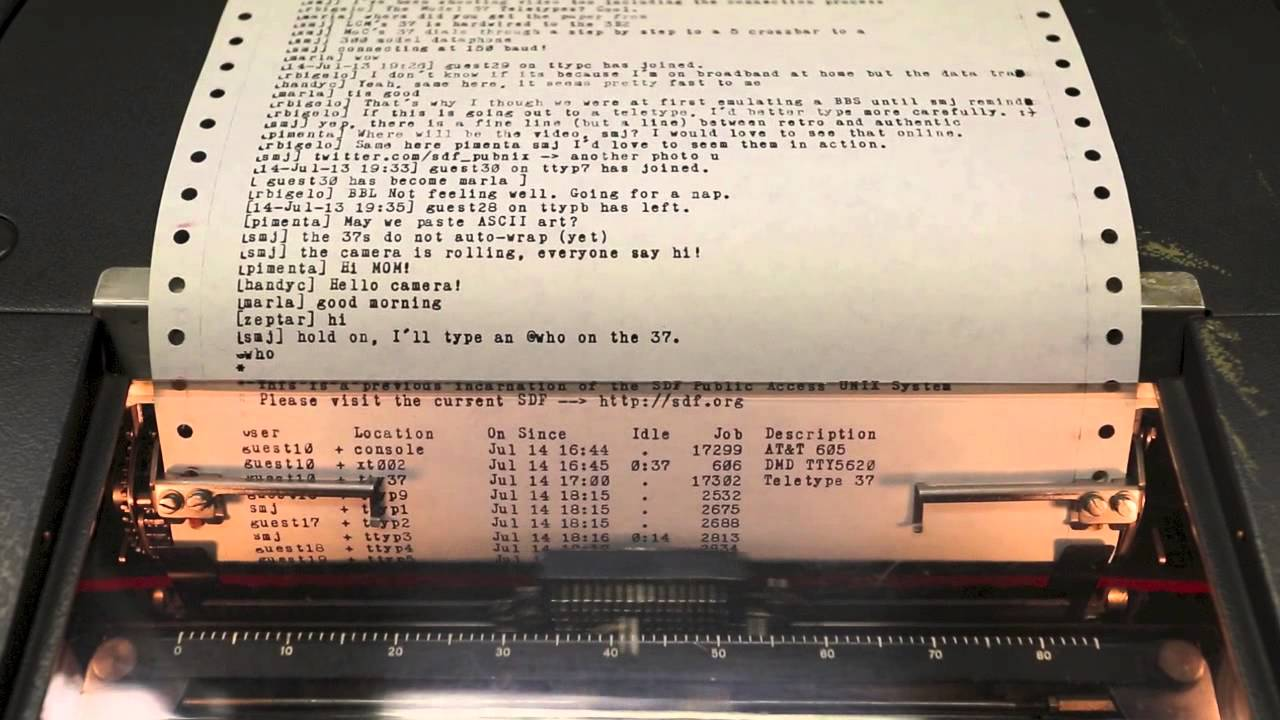
\includegraphics[width=\linewidth]{images/png/tty.png}
  \caption{A Teletype}
	\labfig{tty}
\end{marginfigure}

Very early computers used to use teletypes as the output device.
These were devices that used ink and paper to actually
\textit{print} the output of the computer.
These did not have an \textit{automatic} refresh rate like modern monitors.
Only when the computer sent a signal to the teletype, would the teletype print the output.

Due to these restrictions it was not economical or
practical to print the entire file on the screen.
Thus most editors used to print only one line at a time on the screen
and did not have updating graphics.

\textbf{QED}

\begin{marginfigure}
  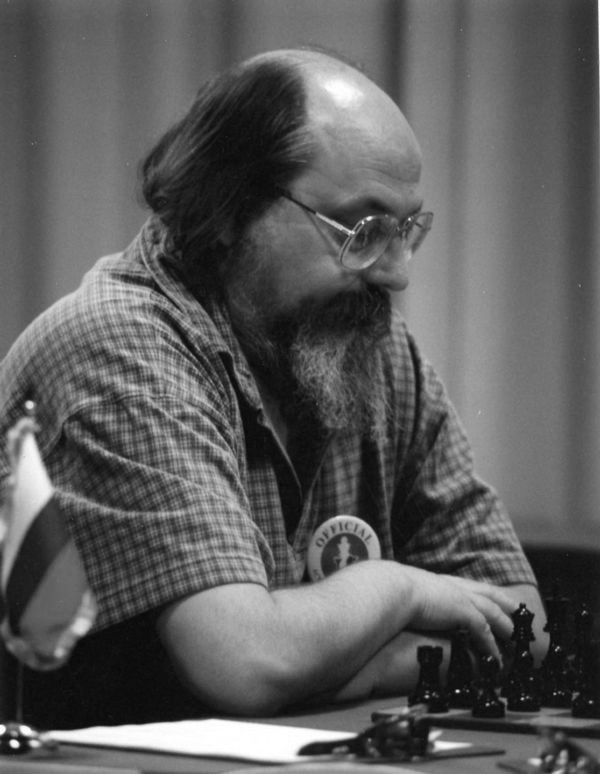
\includegraphics{images/png/thompson.png}
	\caption{Ken Thompson}
	\labfig{thompson}
\end{marginfigure}

QED was a text editor developed by Butler Lampson and Peter Deutsch in 1967 for the Berkeley Timesharing System.
It was a character-oriented editor that was used to create and edit text files.
It used to print or edit only one character at a time on the screen.
This is because the computers at that time used to use
a teletype machine as the output device, and not a monitor.

Ken Thompson used this QED at Berkeley before he came to Bell Labs, and among the first things he did on arriving was to write a new version for the MIT CTSS system.
Written in IBM 7090 assembly language, it differed from the Berkeley version most notably in introducing regular expressions
\sidenote{
  Regular expressions are a sequence of characters that define a search pattern.
  Usually this pattern is used by string searching algorithms for "find" or "find and replace" operations on strings.
  This will be discussed in detail in a later chapter.
}
for specifying strings to seek within the document being edited, and to specify a substring for which a substitution should be made.
Until that time, text editors could search for a literal string, and substitute for one, but not specify more general strings.

Ken not only introduced a new idea, he found an inventive implementation: on-the-fly compiling. Ken's QED compiled machine code for each regular expression that created a NDFA (non-deterministic finite automaton) to do the search. He published this in C. ACM 11 \#6, and also received a patent for the technique: US Patent \#3568156.

\begin{marginfigure}
  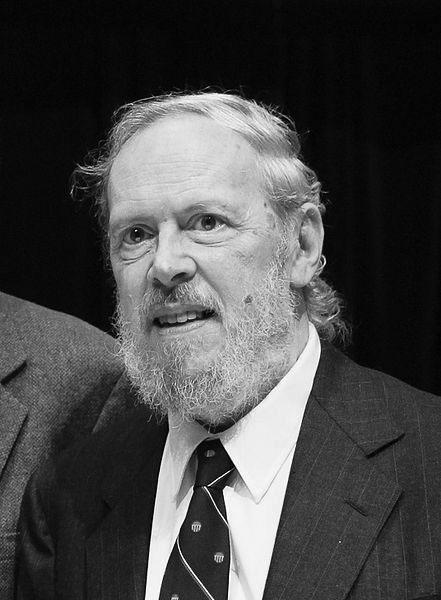
\includegraphics{images/png/ritchie.png}
	\caption{Dennis Ritchie}
	\labfig{ritchie}
\end{marginfigure}

While the Berkeley QED was character-oriented, the CTSS version was line-oriented. Ken's CTSS qed adopted from the Berkeley one the notion of multiple buffers to edit several files simultaneously and to move and copy text among them, and also the idea of executing a given buffer as editor commands, thus providing programmability.

When developing the MULTICS project, Ken Thompson wrote yet another version of QED for that system, now in BCPL
\sidenote{
BCPL ("Basic Combined Programming Language") is a procedural, imperative, and structured programming language. Originally intended for writing compilers for other languages, BCPL is no longer in common use.
}
and now created trees for regular expressions instead of compiling to machine language.

In 1967 when Dennis Ritchie joined the project, Bell Labs had slowly started to move away from Multics. While he was developing the initial stages of Unix, he rewrote QED yet again, this time for the GE-TSS system in Assembly language.
This was well documented, and was originally intented to be published as a paper.
\sidenote{
  At that time, systems did not have a standardized CPU architecture or a generalized low level compiler.
  Due to this, applications were not portable across systems.
  Each machine needed its own version of the application to be written from the scratch, mostly in assembly language.
}

\marginnote{
  The reference manual for GE-TSS QED can still be found on
  \href{https://www.bell-labs.com/usr/dmr/www/qedman.pdf}{Dennis Ritchie's website}
  Much of this information is taken from his
  \href{https://www.bell-labs.com/usr/dmr/www/qed.html}{blog}.
}

\textbf{ED}

After their experience with multiple implementations of QED,
Ken Thompson wrote \textbf{ed} in 1969.

This was now written in the newly developed B language, a predecessor to C.
This implementation was much simpler than QED, and was line oriented.
It stripped out much of regular expression support, and only had the support
for \texttt{*}.
It also got rid of multiple buffers and executing contents of buffer.

Slowly, with time, Dennis Ritchie created the C language, which is widely in use
even today.

Ken Thompson re-wrote \textbf{ed} in C, and added back some of the
complex features of QED, like back references in regular expressions.

Ed ended up being the \textbf{Standard Text Editor} for Unix systems.

\begin{remark}
Since all of Bell-Labs and AT\&T's software was proprietary, the source code for ed was not available to the public.
Thus, the \textit{ed} editor accessible today in \textbf{GNU/Linux},
is another implementation of the original \textit{ed} editor
by the GNU project.
\end{remark}

However, \textbf{ed} was not very user friendly and it was very terse.
Although this was originally intented, since it would be
very slow to print a lot of diagnostic messages on a teletype,
slowly, as people moved to faster computers and monitors,
they wanted a more user friendly editor.

\textbf{VDU Terminals}

\begin{definition}
  A terminal that uses video display technology like
  cathode rat tubes (CRT) or liquid crystal displays (LCD)
  to display the terminal output is called a \textbf{VDU terminal}.
  (Video Display Unit)
\end{definition}

\begin{marginfigure}
  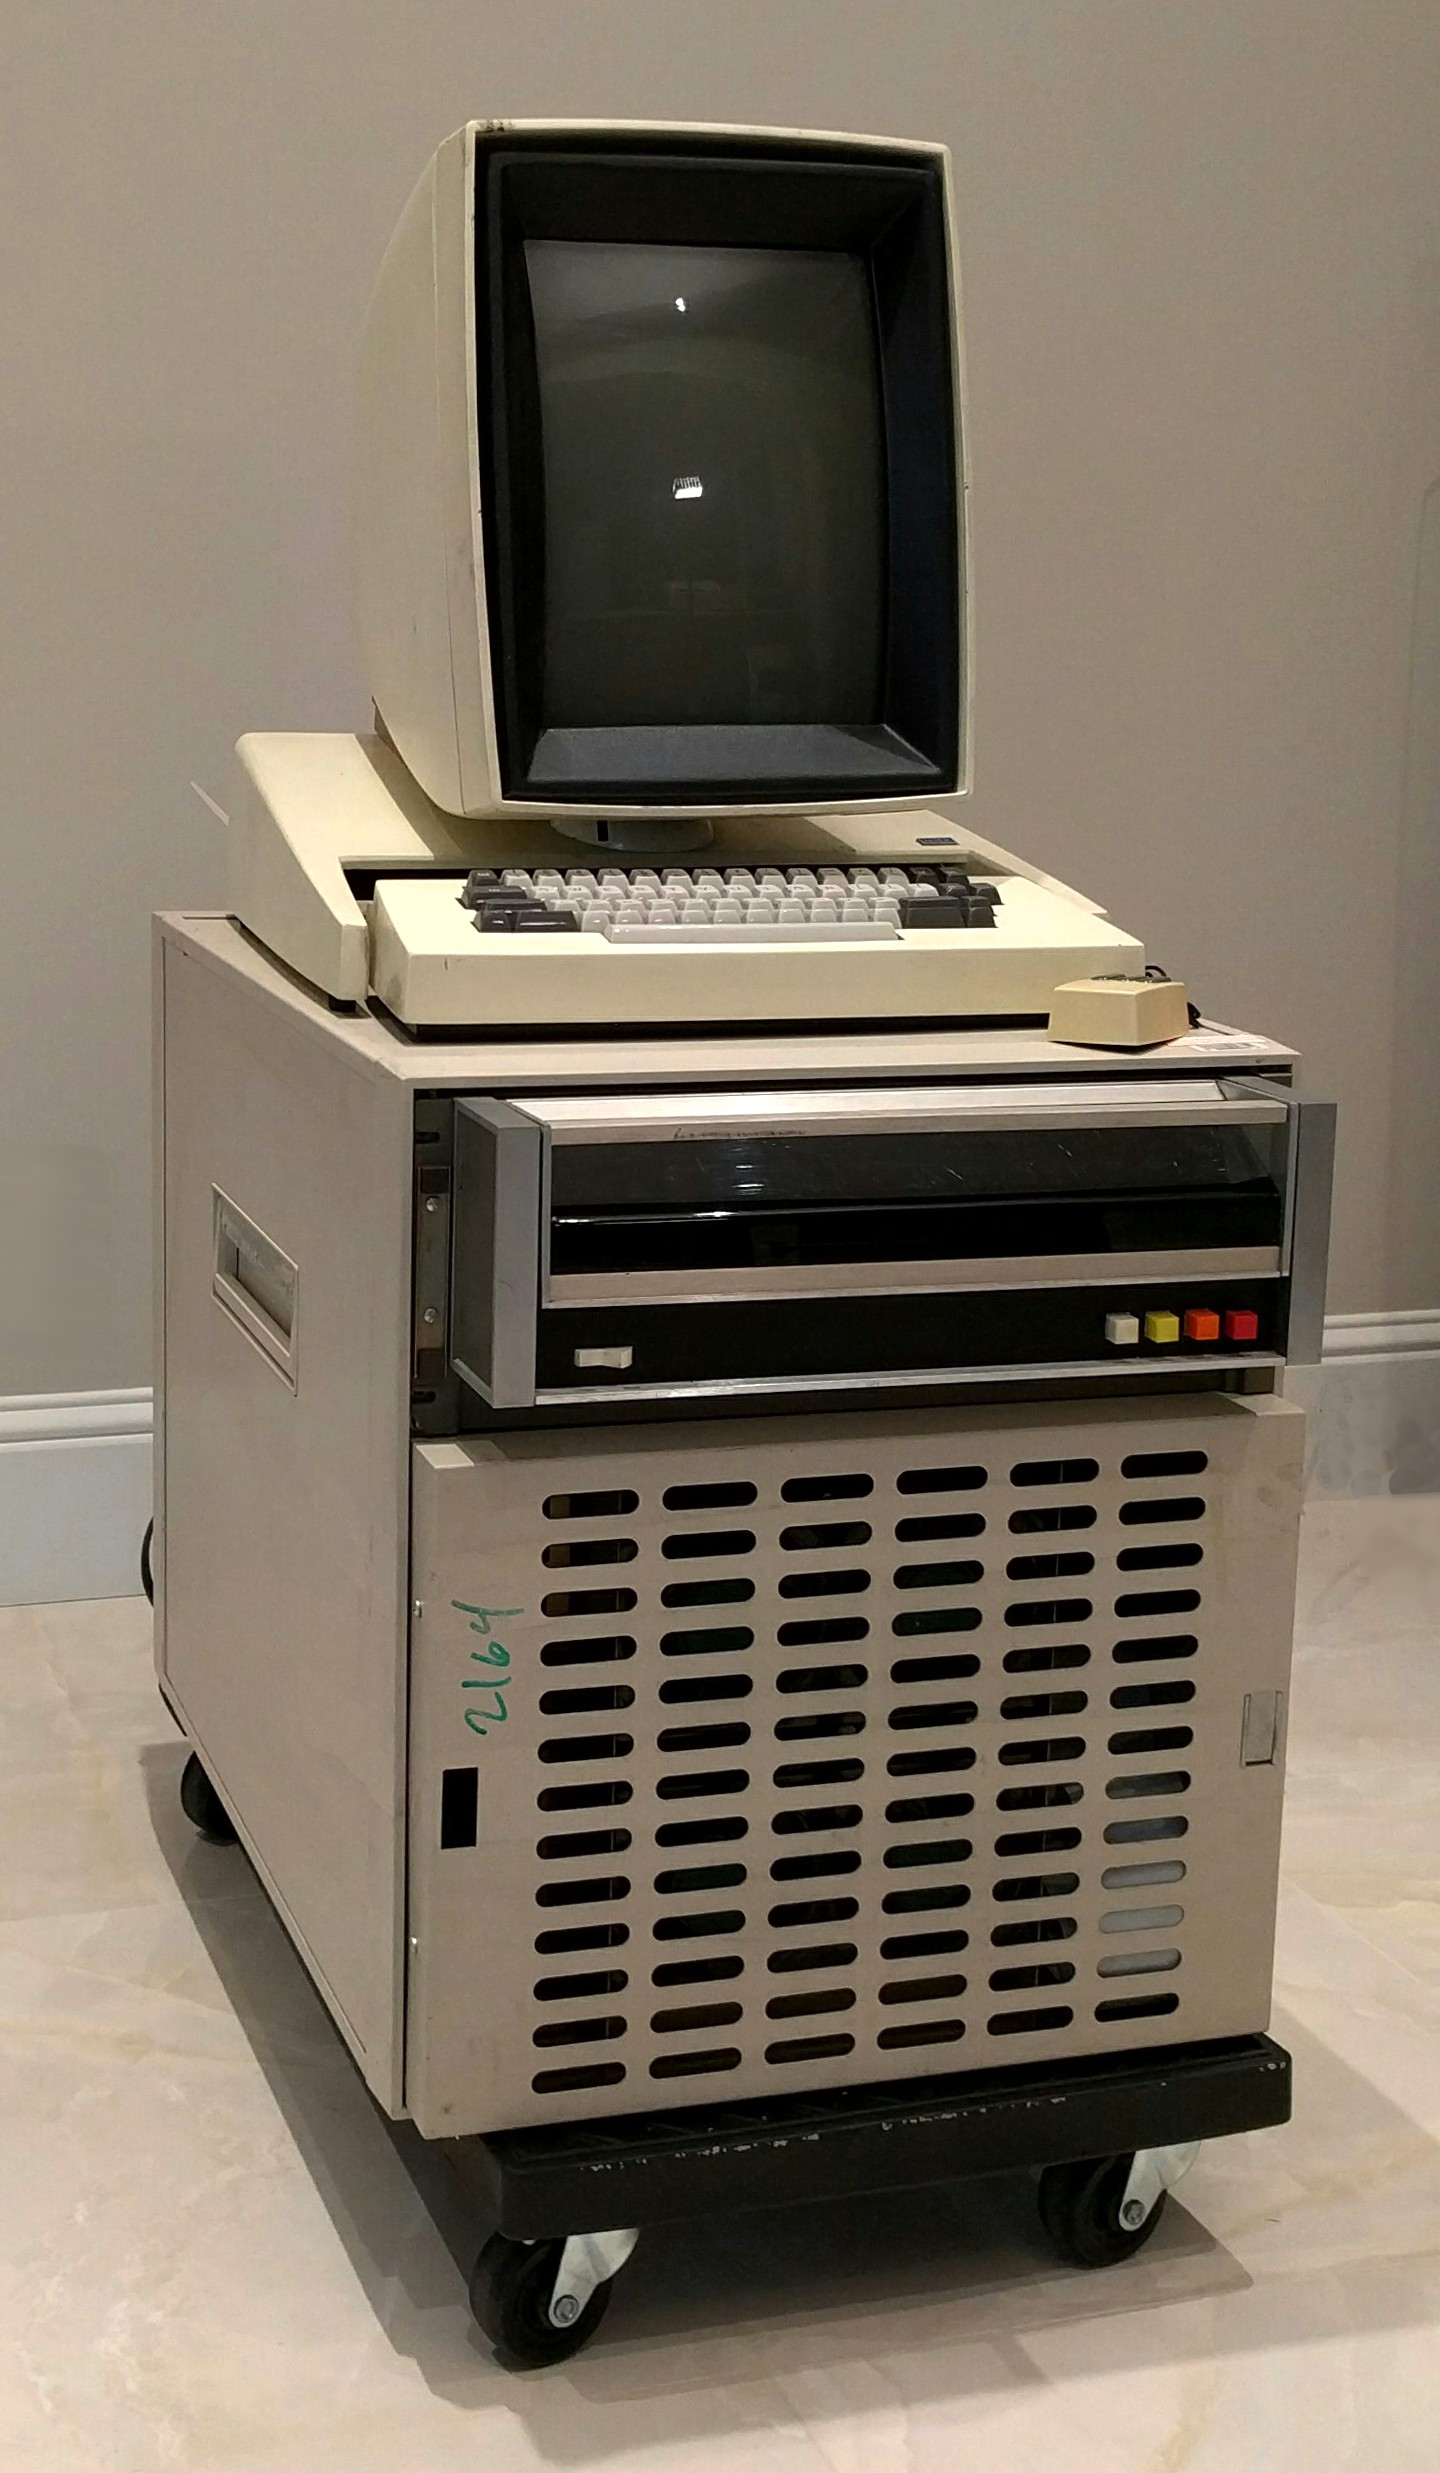
\includegraphics{images/png/alto.png}
  \caption{Xerox Alto, one of the first VDU terminals with a GUI, released in 1973}
	\labfig{alto}
\end{marginfigure}

These terminals were able to show video output, instead of
just printing the output on paper.
Although initially these were very expensive, and were not
a household item, they were present in the research parks
like Xerox PARC.

\textbf{EM}

\href{https://en.wikipedia.org/wiki/George\_Coulouris\_(computer\_scientist)}{George Coulouris}
(not the actor)
was one of the people who had access to these terminals
in his work at the Queen Mary College in London.

The drawbacks of \textbf{ed} were very apparent to him
when using on these machines.

He found that the UNIX's \textbf{raw} mode, which was
at that time totally unused,
could be used to give some of the convenience
and immediacy of feedback for text editing.

He claimed that although the \textbf{ed} editor was
groundbreaking in its time, it was not very user friendly.
He termed it as not being an editor for mortals.

He thus wrote \textbf{em} in 1976, which was an \textbf{Editor for Mortals}.
\sidenote{
  George named em as Editor for Mortals because
  Ken Thompson visited his lab at QMC while he
  was developing it and said something like:
  "yeah, I've seen editors like that,
  but I don't feel a need for them,
  I don't want to see the state of
  the file when I'm editing".
  This made George think that Ken was
  not a mortal, and thus he named it
  Editor for Mortals.
}


\begin{marginfigure}
  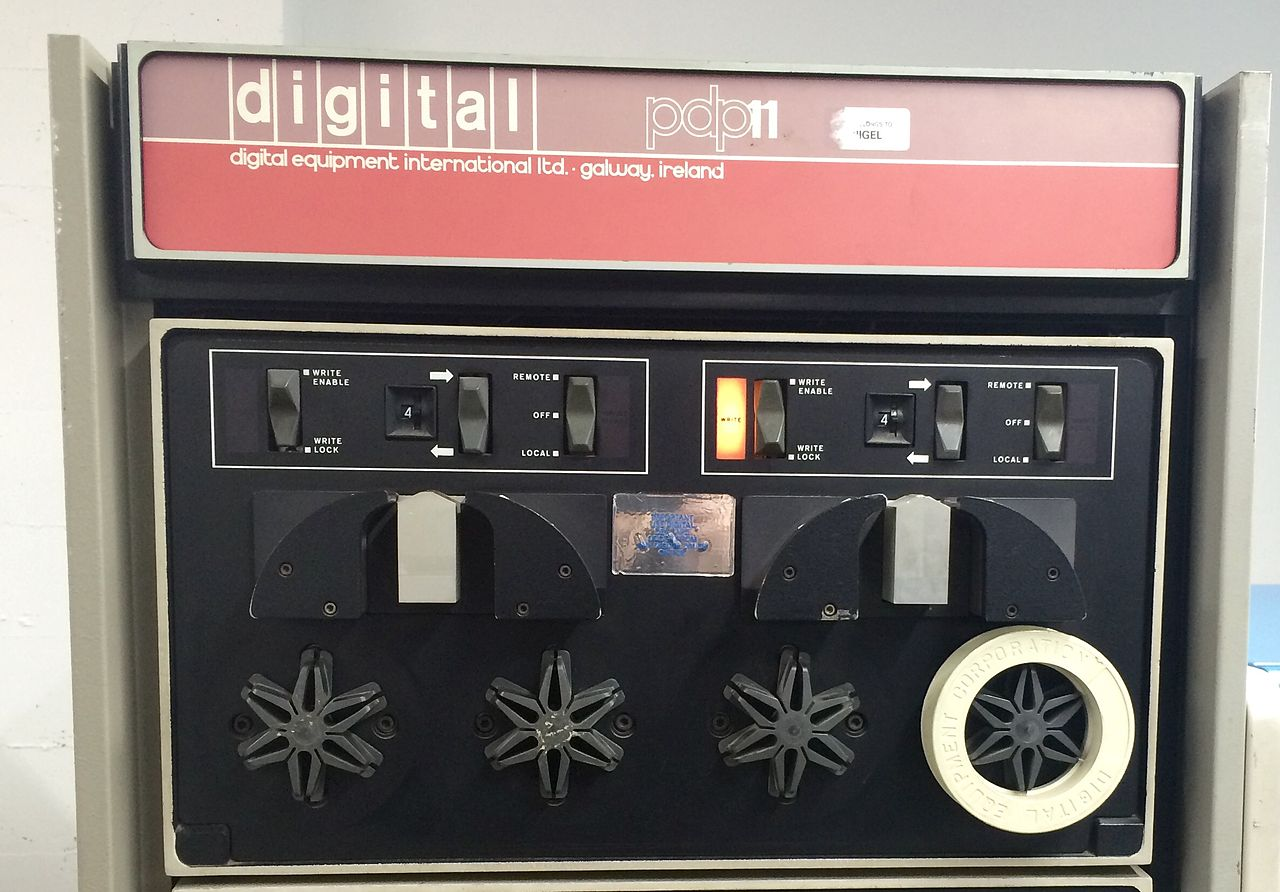
\includegraphics{images/png/dectape-pdp11.png}
  \caption{A first generation Dectape
  (bottom right corner, white round tape)
  being used with a PDP-11 computer}
	\labfig{dectape-pdp11}
\end{marginfigure}

Although em added a lot of features to ed, it was still
a line editor, that is, you could only see one line at a time.
The difference from ed was that it allowed visual editing,
meaning you can see the state of the line as you are editing it.

Whereas most of the development of Multics and Unix
was done in the United States, the development of \textbf{em}
was done in the United Kingdom, in the Queen Mary College,
which was the first college in the UK to have UNIX.

\textbf{EN}

In the summer of 1976, George Coulouris was a visiting professor
at the University of California, Berkeley.
With him, he had brought a copy of his \textbf{em} editor
on a Dectape
\sidenote{
  A Dectape is a magnetic tape storage device that was used in the 1970s.
  It was used to store data and programs.
}
and had installed it there on their departmental computers
which were still using teletype terminals.
Although em was designed for VDU terminals, it was still
able to run (albeit slowly) on the teletype terminals
by printing the current line every time.

\begin{marginfigure}
  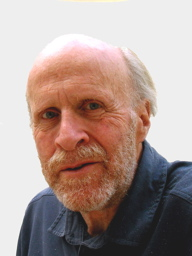
\includegraphics{images/png/georgeQMC.png}
  \caption{George Coulouris}
  \labfig{georgeQMC}
\end{marginfigure}

There he met Bill Joy, who was a PhD student at Berkeley.
On showing him the editor, Bill Joy was very impressed
and wanted to use it on the PDP-11 computers at Berkeley.
The system support team at Berkley were using PDP-11 which
used VDU Terminals, an environment where em would really shine.

He explained that 'em' was an extension of 'ed'
that gave key-stroke level interaction for editing
within a single line, displaying the up-to-date line
on the screen (a sort of single-line screen editor).
This was achieved by setting the terminal mode to 'raw'
so that single characters could be read as they were typed
- an eccentric thing for a program to do in 1976.

Although the system support team at Berkeley were
impressed by this editor, they knew that if this
was made available to the general public, it would
take up too much resources by going to the raw mode
on every keypress.
But Bill and the team took a copy of the source code
just to see if they might use it.

George then took a vacation for a few weeks,
but when he returned, he found that Bill had
taken his ex as a starting point and had
added a lot of features to it. He called it
\textbf{en} initially, which later became \textbf{ex}.

\textbf{EX}

\begin{marginfigure}
  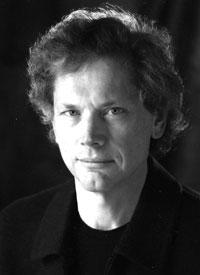
\includegraphics{images/png/billjoy.png}
  \caption{Bill Joy}
  \labfig{billjoy}
\end{marginfigure}


Bill Joy took inspiration from several other ed clones as well,
and their own tweaks to ed,
although the primary inspiration was \textbf{em}.
Bill and Chuck Haley built upon em to make en, which later became ex.

This editor had a lot of improvements over em,
such as adding the ability to add abbreviations
(using the \texttt{ab} command),
and adding keybindings (maps).

It also added the ability to mark some line
using the \texttt{k} key followed by any letter,
and then jump to that line from any arbitrary line
using the \texttt{'} key followed by the letter.

Slowly, with time, the modern systems were able able
to handle the raw mode, and real time editing more and more.
This led to the natural progression, What if we could
see the entire file at once, and not just one line at a time?

\textbf{VI}

Bill added the \textbf{visual mode} to ex in 1977.
\sidenote{
  This visual mode is not the same as the visual mode in vim.
}
This was not a separate editor, but rather just another mode
of the \textbf{ex} editor.
You could open ex in visual mode using the \texttt{-v} flag to
ex.

\begin{lstlisting}[language=bash]
$ ex -v filename
\end{lstlisting}

This visual mode was the first time a text editor
was \textbf{modal}.
This means that the editor had different modes for different tasks.
When you want to edit text, you would go to the insert mode,
and type the text.
When you want to navigate, you would go to the normal mode,
and use the navigation keys and other motions defined in vi.

Slowly, as the visual mode became more and more popular,
Bill added a hardlink to ex called \textbf{vi}.
\sidenote{
  This means that it did not take up additional space on the disk,
  but was just another entry in the directory entry that pointed
  to the same inode which stored the ex binary path.
  Upon execution, \textbf{ex} would detect if it was
  called as \textbf{vi} and would start in visual mode by default.
  We have covered hardlinks in \refch{basic}.
}

The modal version of vi was also inspired from another
editor called \textbf{bravo}, which was developed at Xerox PARC.
\sidenote{
  Xerox PARC has always been ahead of its time.
  The first graphical user interface was developed at Xerox PARC.
  The bravo editor used bitmapped graphics to display the text,
  and had extensive mouse support.
  The overdependence on the mouse in such an early time
  was one of the reasons that the bravo editor was not
  as popular as vi.
}

If you use vi/vim, you may notice that the key to
exit the insert mode is \texttt{Esc}.
This may seem inconveniently placed at the top left corner,
but this was because the original vi was developed on a
ADM-3A terminal, which had the \texttt{Esc} key to the left
of the \textbf{Q} key, where modern keyboards have the \texttt{Tab} key.
\sidenote{
  Since the placement of the Escape key is inconvenient
  in modern keyboard layouts, many people remap the
  Escape key to the \texttt{Caps Lock} key either in vim
  or in the operating system itself.
}

Also, the choice of h,j,k,l for navigation was because
the ADM-3A terminal did not have arrow keys,
rather, it had h,j,k,l keys for navigation.

This can be seen in \reffig{adm3a}.

\begin{figure}[h!]
  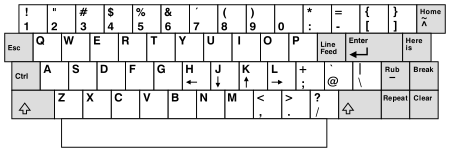
\includegraphics{images/png/adm3a.png}
  \caption{The Keyboard layout of the ADM-3A terminal}
  \labfig{adm3a}
\end{figure}


Bill Joy was also one of the people working on the
\textbf{Berkeley Software Distribution (BSD) of Unix}.
Thus he bundled vi with the first BSD distribution of UNIX
released in 1978.
The pre-installed nature of vi in the BSD Distribution
made it very popular.

However, since both the source code of ed was restricted by
Bell Labs - AT\&T, and the source code of vi was restricted
by the University of California, Berkeley,
they could not be modified by the users or distributed freely.

This gave birth to a lot of clones of vi.

\textbf{Vi Clones}

The vi clones were written because the source code for the original version was not freely available until recently. This made it impossible to extend the functionality of vi. It also precluded porting vi to other operating systems, including Linux.

\begin{marginfigure}
  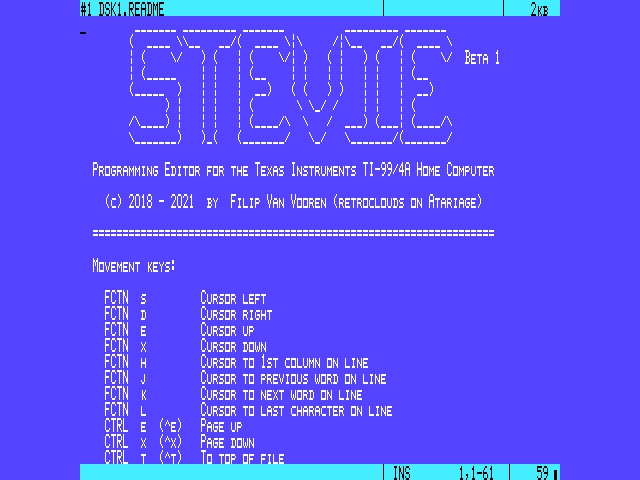
\includegraphics{images/png/stevie.png}
  \caption{Stevie Editor}
  \labfig{stevie}
\end{marginfigure}

\begin{itemize}
  \item \textbf{calvin}: a freeware "partial clone of vi" for use on MS-DOS.
 It has the advantages of small size (the .exe file is only 46.1KB!) and fast execution but the disadvantage that it lacks many of the ex commands, such as search and replace.
  \item \textbf{lemmy}: a shareware version of vi implemented for the Microsoft Windows platforms which combines the interface of vi with the look and feel of a Windows application.
  \item \textbf{nvi}: It is a re-implementation of the classic Berkeley vi editor, derived from the original 4.4BSD version of vi.
    It is the "official" Berkeley clone of vi, and it is included in FreeBSD and the other BSD variants.
  \item \textbf{stevie}: `ST Editor for VI Enthusiasts` was developed by Tim Thompson for the Atari ST.
    It is a clone of vi that runs on the Atari ST.
    Tim Thompson wrote the code from scratch (not based on vi) and posted its
    source code as a free software to
    \href{https://groups.google.com/g/comp.sys.atari.st}{comp.sys.atari.st}
    on June 1987. Later it was ported to UNIX, OS/2, and Amiga.
    Because of this independence from vi and ed's closed source license,
    most vi clones would base their work off of stevie to keep it free
    and open source.
  \item \textbf{elvis}:
    Elvis creator, Steve Kirkendall, started thinking of writing his own editor after Stevie crashed on him, causing him to lose hours of work and damaging his confidence in the editor.
Stevie stored the edit buffer in RAM, which Kirkendall believed to be impractical on the MINIX operating system. One of Kirkendall's main motivation for writing his own vi clone was that his new editor stored the edit buffer in a file instead of storing it in RAM. Therefore, even if his editor crashed, the edited text could still be retrieved from that external file.
Elvis was one of the first vi clones to offer support for GUI and syntax highlighting.
\end{itemize}

The clones add numerous new features which make them significantly easier to use than the original vi, especially for neophytes.
A particularly useful feature in many of them is the ability to edit files in multiple windows.
This facilitates working on more than one file at the same time, including cutting and pasting text among them.

Many of the clones also offer GUI versions of vi that operate under the X Windows system and can take advantage of bit-mapped (high resolution) displays and the mouse.

\textbf{Vim}

\begin{marginfigure}
  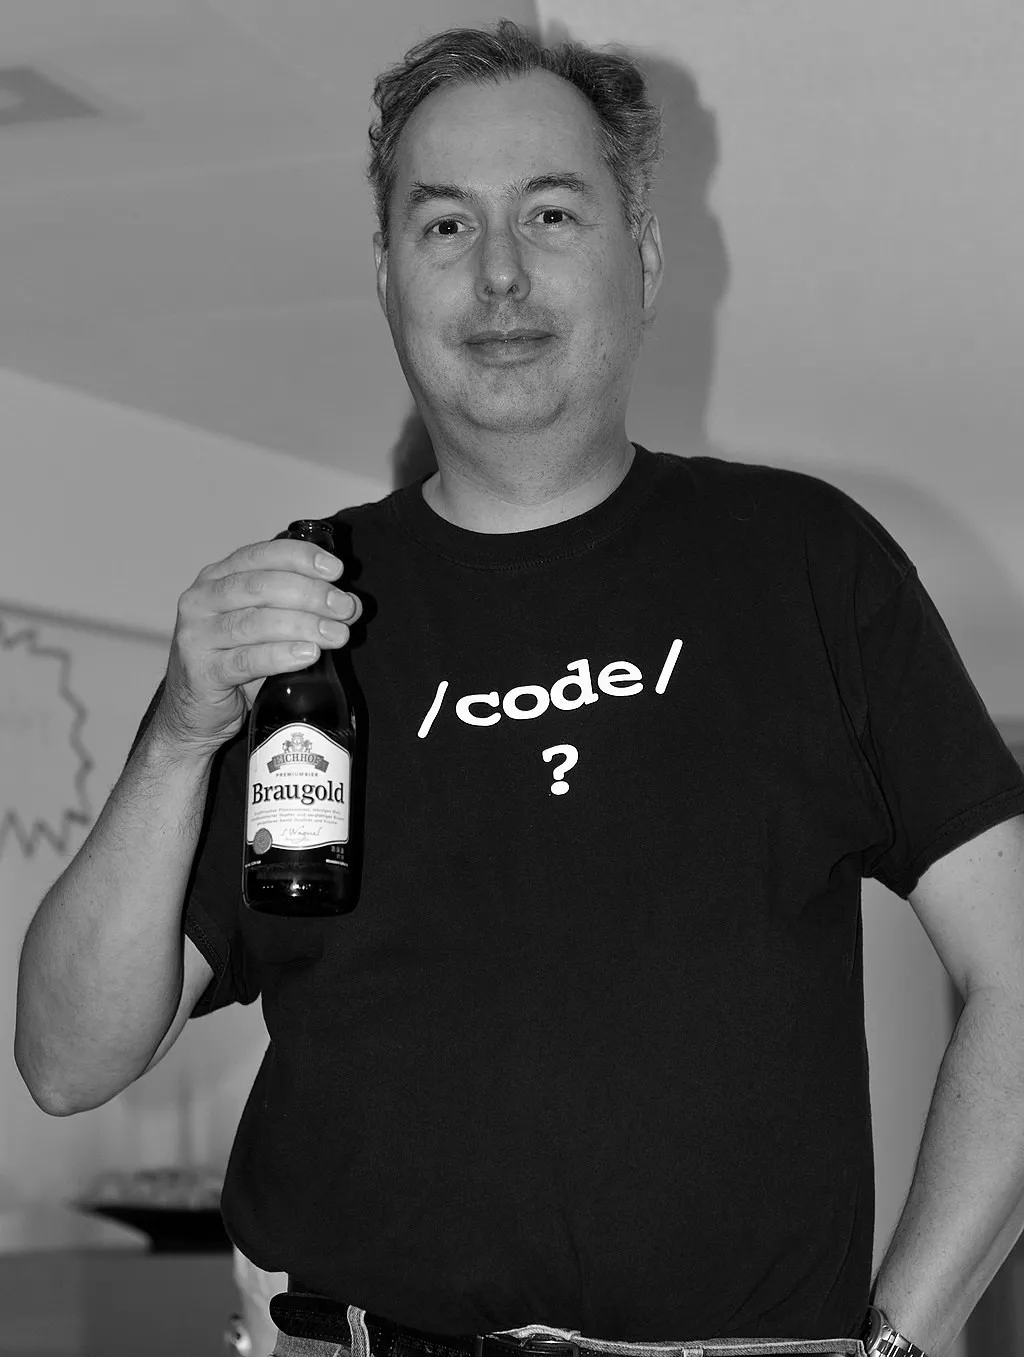
\includegraphics{images/png/bram.png}
  \caption{Bram Moolenaar}
  \labfig{bram}
\end{marginfigure}

Bram Moolenaar, a Dutch programmer, was impressed by
STeVIe, a vi clone for the Atari ST.
But he was working with the Commodore Amiga at that time,
and there was no vi clone for the Amiga.
So Bram began working on the stevie clone
for the AmigaOS in 1988.

\begin{figure}[h!]
  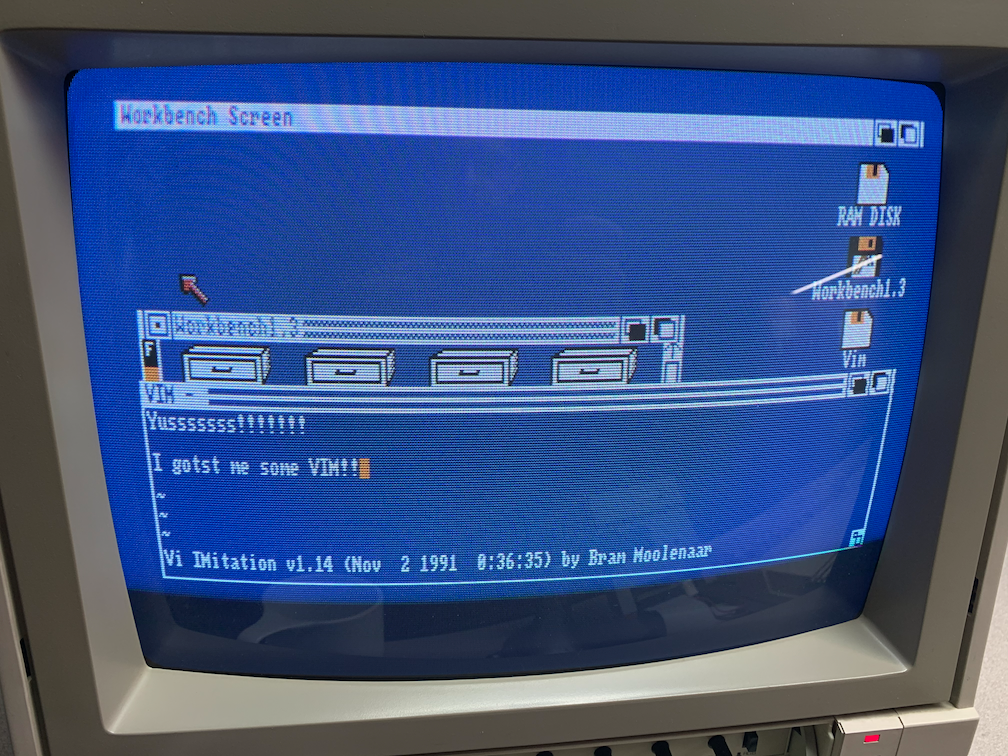
\includegraphics[width=0.8\linewidth]{images/png/vim-amiga.png}
  \caption{The inital version of Vim, when it was called Vi IMitation}
  \labfig{vim-amiga}
\end{figure}

He released the first public release (v 1.14) in 1991
as visible in \reffig{vim-amiga}.

Since Vim was based off of Stevie, and not ed or vi
so it could be freely distributed.
It was licensed under a charityware license,
named as Vim License.
The license stated that if you liked the software,
you should consider making a donation to a charity
of your choice.

Moolenaar was an advocate of a NGO based in Kibaale, Uganda,
which he founded to support children whose parents have died of AIDS.
In 1994, he volunteered as a water and sanitation engineer for the
Kibaale Children's Centre and made several return trips
over the following twenty-five years.

Later Vim was re-branded as `Vi IMproved`
as seen in \reffig{vim}.

\begin{marginfigure}
  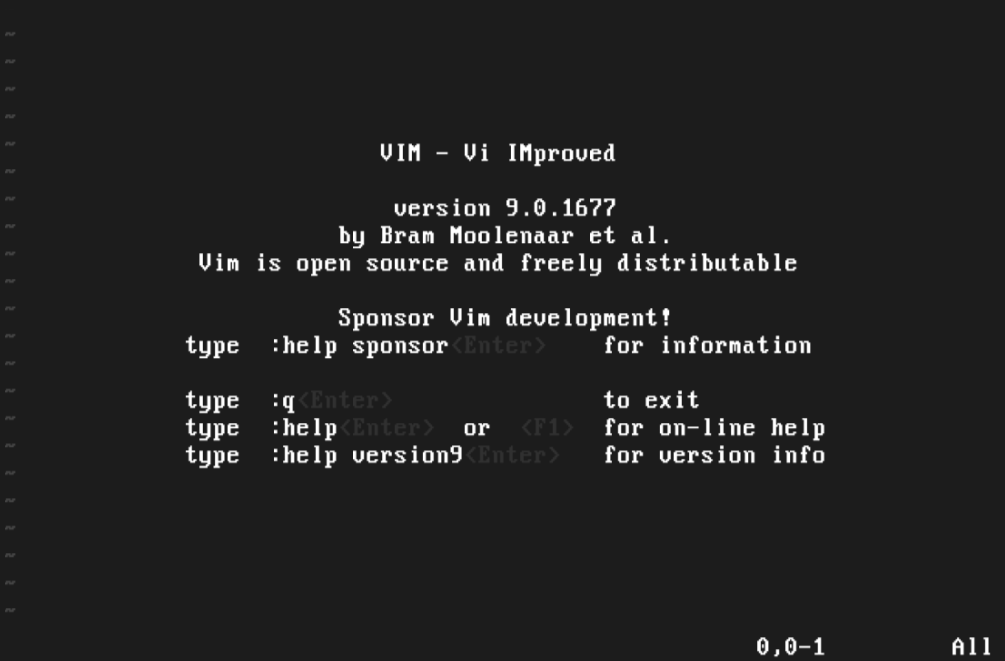
\includegraphics{images/png/vim.png}
  \caption{Vim 9.0 Start screen}
  \labfig{vim}
\end{marginfigure}

Vim has been in development for over 30 years now,
and is still actively maintained.
It has added a lot of features over the years,
such as syntax highlighting, plugins,
completion, PCRE support, mouse support, etc.

\textbf{neovim}

Recently there have been efforts
to modernize the vim codebase.
Since it is more than 30 years old,
it has a lot of legacy code.
The scripting language of vim is
also not a standard programming language,
but rather a custom language called vimscript.

To counter this, a new project called \textbf{neovim}
has been started.
It uses \textbf{lua} as the scripting language,
and has a lot of modern features like
out of the box support for LSP,
\sidenote{
  LSP stands for Language Server Protocol.
  It is a protocol that allows the editor to communicate
  with a language server to provide features like
  autocompletion, go to definition, etc.
  This makes vim more like an IDE.
}
better mouse integration, etc.

In this course, we will be learning only
about basic vi commands and we will be
using vim as the editor.

\begin{figure}[h!]
  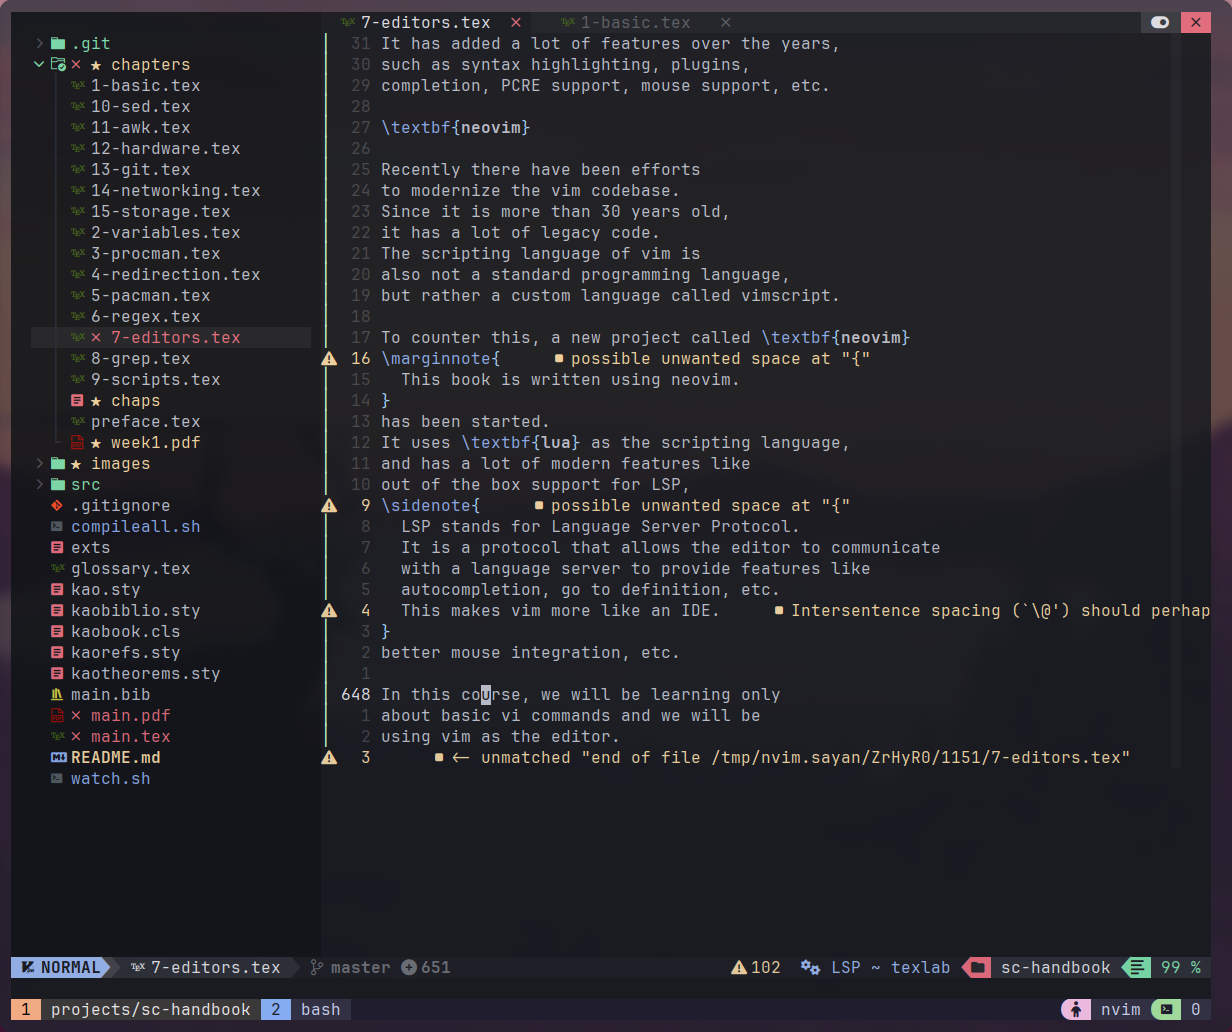
\includegraphics{images/png/nvim.png}
  \caption{Neo Vim Window editing this book}
  \labfig{nvim}
\end{figure}

\marginnote{
  This book is written using neovim.
}

\vfill
\pagebreak

\subsection{Ed Commands}

Before we move on to Vi Commands,
let us first learn about the basic ed commands.
These will also be useful in vim, since the
ex mode of vim is based on ed/ex where we can
directly use ed commands on our file in the buffer.

\begin{table}[h!]
  \caption{Ed Commands}
  \labtab{edcommands}
  \begin{tabular}{l l}
    \toprule
    Description & Commands \\
    \midrule
    Show the \textbf{P}rompt & \texttt{P} \\
    Command Format & \texttt{[addr[,addr]]cmd[params]} \\
    Commands for location & \texttt{1} \texttt{.} \texttt{\$} \texttt{\%} \texttt{+} \texttt{-} \texttt{,} \texttt{;} \texttt{/RE/} \\
    Commands for editing & \texttt{f} \texttt{p} \texttt{a} \texttt{c} \texttt{d} \texttt{i} \texttt{j} \texttt{s} \texttt{m} \texttt{u} \\
    Execute a shell \textit{command} & \texttt{!command} \\
    \textbf{e}dit a file & \texttt{e filename} \\
    \textbf{r}ead file contents into buffer & \texttt{r filename} \\
    \textbf{r}ead \textit{command} output into buffer & \texttt{r !command} \\
    \textbf{w}rite buffer to filename & \texttt{w filename} \\
    \textbf{q}uit & \texttt{q} \\
    \bottomrule
  \end{tabular}
\end{table}

\textbf{Commands for location}

\begin{table}[h!]
  \caption{Commands for location}
  \labtab{ed-location}
\begin{tabular}{ c l }
\toprule
Commands & Description \\
\midrule
a number like \texttt{2} & refers to second line of file \\
\texttt{.} & refers to current line \\
\texttt{\$} & refers to last line \\
\texttt{\%} & refers to all the lines \\
\texttt{+} & line after the cursor (current line) \\
\texttt{-} & line before the cursor (current line) \\
\texttt{,} & refers to buffer holding the file or last line in buffer \\
\texttt{;} & refers to current position to end of the file \\
\texttt{/RE/} & refers line matched by pattern specified by 'RE' \\
\bottomrule
\end{tabular}
\end{table}


\textbf{Commands for Editing}

\begin{table}[h!]
  \caption{Commands for Editing}
  \labtab{ed-editing}
  \begin{tabular}{ c l }
    \toprule
    Commands & Description \\
    \midrule
    \texttt{f} & show name of \textbf{f}ile being edited \\
    \texttt{p} & \textbf{p}rint the current line \\
    \texttt{a} & \textbf{a}ppend at the current line \\
    \texttt{c} & \textbf{c}hange the current line \\
    \texttt{d} & \textbf{d}elete the current line \\
    \texttt{i} & \textbf{i}nsert line at the current position \\
    \texttt{j} & \textbf{j}oin lines \\
    \texttt{s} & \textbf{s}earch for regex pattern \\
    \texttt{m} & \textbf{m}ove current line to position \\
    \texttt{u} & \textbf{u}ndo latest change \\
    \bottomrule
  \end{tabular}
\end{table}

Let us try out some of these commands in the ed editor.

Lets start with creating a file, which we will then open
in the ed editor.

\begin{lstlisting}[language=bash]
$ echo "line-1 hello world
line-2 welcome to line editor
line-3 ed is perhaps the oldest editor out there
line-4 end of file" > test.txt
\end{lstlisting}

This creates a file in the current working directory
with the name \texttt{test.txt} and the contents as
given above.

We invoke ed by using the executable \texttt{ed}
and providing the filename as an argument.

\begin{lstlisting}[language=bash]
$ ed test.txt
117
\end{lstlisting}

As soon as we run it, you will see a number,
which is the number of characters in the file.
The terminal may seem hung, since there is no
prompt, of either the bash shell, or of the ed editor.
This is because ed is a line editor, and it does not
print the contents of the file on the screen.

Off the bat, we can observe the terseness of the ed editor
since it does not even print a prompt.
To turn it on, we can use the \texttt{P} command.
The default prompt is \texttt{*}.

\begin{lstlisting}[language=bash]
ed test.txt
117
P
*
\end{lstlisting}

Now we can see the prompt \texttt{*} is always present,
whenever the ed editor expects a command from the user.

Lets go to the first line of the file using the \texttt{1} command.
We can also go to the last line of the file using the \texttt{\$} command.

\begin{lstlisting}[language=bash]
*1
line-1 hello world
*$
line-4 end of file
*
\end{lstlisting}

To print out all the lines of the file,
we can use the \texttt{,} or \texttt{\%} with \texttt{p} command.

\begin{lstlisting}[language=bash]
*,p
line-1 hello world
line-2 welcome to line editor
line-3 ed is perhaps the oldest editor out there
line-4 end of file
\end{lstlisting}

\begin{lstlisting}[language=bash]
*%p
line-1 hello world
line-2 welcome to line editor
line-3 ed is perhaps the oldest editor out there
line-4 end of file
\end{lstlisting}

However, if we use the \texttt{,} command without
the \texttt{p} command, it will not print all the lines.
Rather, it will just move the cursor to the last line
and print the last line.

\begin{lstlisting}[language=bash]
*,
line-4 end of file
\end{lstlisting}

We can also print any arbitrary line range
using the line numbers separated by a comma
and followed by the \texttt{p} command.

\begin{lstlisting}[language=bash]
*2,3p
line-2 welcome to line editor
line-3 ed is perhaps the oldest editor out there
\end{lstlisting}

One of the pioneering features of ed was the ability
to search for a pattern in the file. Let us quickly
explain the syntax of the search command.
\sidenote{
  The details of regular expressions will be covered in a later chapter.
}

\begin{lstlisting}[language=bash]
*/hello/
line-1 hello world
\end{lstlisting}

We may or may not include the \texttt{p} command
after the last \texttt{/{}} in the search command.

We can advance to the next line using the \texttt{+} command.

\begin{lstlisting}[language=bash]
*p
line-1 hello world
*+
line-2 welcome to line editor
\end{lstlisting}

And go to the previous line using the \texttt{-} command.


\begin{lstlisting}[language=bash]
*p
line-2 welcome to line editor
*-
line-1 hello world
\end{lstlisting}

We can also print all the lines from the current line
to the end of the file using the \texttt{;p} command.

\begin{lstlisting}[language=bash]
*.
line-2 welcome to line editor
*;p
line-2 welcome to line editor
line-3 ed is perhaps the oldest editor out there
line-4 end of file
\end{lstlisting}

We can also run arbitrary shell commands using the \texttt{!} command.

\begin{lstlisting}[language=bash]
*! date
Mon Jun 10 11:36:34 PM IST 2024
!
\end{lstlisting}

The output of the command is shown to the screen,
however, it is not saved in the buffer.

To read the output of a command into the buffer,
we can use the \texttt{r} command.

\begin{lstlisting}[language=bash]
*r !date
32
*%p
line-1 hello world
line-2 welcome to line editor
line-3 ed is perhaps the oldest editor out there
line-4 end of file
Mon Jun 10 11:37:42 PM IST 2024
\end{lstlisting}

The output after running the \texttt{r !date} command
is the number of characters read into the buffer.
We can then print the entire buffer using the \texttt{\%p} command.

The read data is appended to the end of the file.

We can write the buffer
\sidenote{
  Remember that the buffer is the in-memory copy of the file
  and any changes made to the buffer are not saved to the file
  until we write the buffer to the file.
}
to the disk using the \texttt{w} command.

\begin{lstlisting}[language=bash]
*w
149
\end{lstlisting}

The output of the \texttt{w} command is the number of characters written to the file.

To exit ed, we can use the \texttt{q} command.

\begin{lstlisting}[language=bash]
*q
\end{lstlisting}

To delete a line, we can use the \texttt{d} command.
Lets say we do not want the date output in the file.
We can re-open the file in ed and remove the last line.

\begin{lstlisting}[language=bash]
$ ed test.txt
149
P
*$
Mon Jun 10 11:38:49 PM IST 2024
*d
*%p
line-1 hello world
line-2 welcome to line editor
line-3 ed is perhaps the oldest editor out there
line-4 end of file
*wq
117
\end{lstlisting}

We can add lines to the file using the \texttt{a} command.
This appends the line after the current line.
On entering this mode, the editor will keep on taking
input for as many lines as we want to add.
To end the input, we can use the \texttt{.} command on a new line.

\begin{lstlisting}[language=bash]
$ ed test.txt
117
P
*3
line-3 ed is perhaps the oldest editor out there
*a
perhaps not, since we know it was inspired from QED
which was made multiple times by thompson and ritchie
before ed was made.
.
*%p
line-1 hello world
line-2 welcome to line editor
line-3 ed is perhaps the oldest editor out there
perhaps not, since we know it was inspired from QED
which was made multiple times by thompson and ritchie
before ed was made.
line-4 end of file
*
\end{lstlisting}

We can also utilize the regular expression support
in ed to perform search and replace operations.
This lets us either search for a fixed string
and replace with another fixed string, or search
for a pattern and replace it with a fixed string.

Let us change hello world to hello universe.

\begin{lstlisting}[language=bash]
*1
line-1 hello world
*s/world/universe/
line-1 hello universe
*%p
line-1 hello universe
line-2 welcome to line editor
line-3 ed is perhaps the oldest editor out there
perhaps not, since we know it was inspired from QED
which was made multiple times by thompson and ritchie
before ed was made.
line-4 end of file
*
\end{lstlisting}

We can print the name of the currently opened file
using the \texttt{f} command.

\begin{lstlisting}[language=bash]
*f
test.txt
\end{lstlisting}

If we wish to join two lines, we can use the \texttt{j} command.
Let us join lines 4,5, and 6.

\begin{lstlisting}[language=bash]
*4
perhaps not, since we know it was inspired from QED
*5
which was made multiple times by thompson and ritchie
*6
before ed was made.
*4,5j
*4
perhaps not, since we know it was inspired from QEDwhich was made multiple times by thompson and ritchie
*5
before ed was made.
*4,5j
*4
perhaps not, since we know it was inspired from QEDwhich was made multiple times by thompson and ritchiebefore ed was made.
*
\end{lstlisting}

Here we can see that we do the joining in two steps,
first the lines 4 and 5 are joined,
and then the newly modified line 4 and 5 are joined.

We can move a line from its current position to another
line using the \texttt{m} command.

Lets insert a line-0 at the end of the file
and then move it to the beginning of the file.

\begin{lstlisting}[language=bash]
*7
line-4 end of file
*a
line-0 in the beginning, there was light
.
*8
line-0 in the beginning, there was light
*m0
*1,4p
line-0 in the beginning, there was light
line-1 hello universe
line-2 welcome to line editor
line-3 ed is perhaps the oldest editor out there
*
\end{lstlisting}

We can also undo the last change using the \texttt{u} command.
\sidenote{
  The undo command in ed is not as powerful as the undo command in vim.
  In vim, we can undo multiple changes using the \texttt{u} command.
  In ed, we can only undo the last change.
  If we run the \texttt{u} command multiple times,
  it will undo the last change of undoing the last change,
  basically redoing the last change.
}

\begin{lstlisting}[language=bash]
*1
line-0 in the beginning, there was light
*s/light/darkness
line-0 in the beginning, there was darkness
*u
*.
line-0 in the beginning, there was light
*
\end{lstlisting}

If search and replace is not exactly what we want, and
we want to totally change the line, we can use the \texttt{c} command.
It will let us type a new line, which will replace the current line.

\begin{lstlisting}[language=bash]
*%p
line-0 in the beginning, there was light
line-1 hello universe
line-2 welcome to line editor
line-3 ed is perhaps the oldest editor out there
perhaps not, since we know it was inspired from QEDwhich was made multiple times by thompson and ritchiebefore ed was made.
line-4 end of file
*4
line-3 ed is perhaps the oldest editor out there
*c
line-4 ed is the standard editor for UNIX
.
*4
line-4 ed is the standard editor for UNIX
*
\end{lstlisting}

Just like the \texttt{a} command, we can also use the \texttt{i} command
to insert a line at the current position. This will move the current line
to the next line.

\begin{lstlisting}[language=bash]
*6
line-4 end of file
*i
before end of file
.
*6,$p
before end of file
line-4 end of file
*
\end{lstlisting}

Finally, we can also number the lines using the \texttt{n} command.

\begin{lstlisting}[language=bash]
*%p
line-0 in the beginning, there was light
line-1 hello universe
line-2 welcome to line editor
line-4 ed is the standard editor for UNIX
perhaps not, since we know it was inspired from QEDwhich was made multiple times by thompson and ritchiebefore ed was made.
before end of file
line-4 end of file
*%n
1       line-0 in the beginning, there was light
2       line-1 hello universe
3       line-2 welcome to line editor
4       line-4 ed is the standard editor for UNIX
5       perhaps not, since we know it was inspired from QEDwhich was made multiple times by thompson and ritchiebefore ed was made.
6       before end of file
7       line-4 end of file
*
\end{lstlisting}

\vfill
\pagebreak
\subsection{Exploring Vim}

There are a plethora of commands in vim.
We wont be able to cover all of them in this course.
Only the basic commands required to get started
with using vim as your primary editor would be
covered. A detailed tutorial on vim can be found
by running the command \texttt{vimtutor} in your terminal.

\begin{lstlisting}
$ vimtutor
\end{lstlisting}

This opens a temporary files that goes through a lot of
sections of vim, explaining the commands in detail.
This opens the text file in vim itself, so you can
actually try out each exercise as and when you read it.
Many exercises are present in this file to help you
remember and master commands. Feel free to modify the
file since it is a temporary file and any changes made
is lost if the command is re-run.

To open a file in vim, we provide the filename as an argument
to the vim executable.

\begin{lstlisting}[language=bash]
$ vim test.txt
\end{lstlisting}


\textbf{Modal Editor}

\marginnote{
  Sometimes the normal mode is called command mode
  or escape mode, since we can run commands in this mode
  and we press the \texttt{Esc} key to go to this mode.
  However, the ex mode is also called command mode,
  since we can run ex commands in this mode.
  To avoid confusions, we will refer to the navigational(default)
  mode as normal mode, since vim internally also refers to it as
  normal mode, and we will refer to the ex mode as ex mode.
}

Vim is a modal editor, which means that it has different modes
that it operates in. The primary modes are:

\begin{itemize}
  \item Normal/Command Mode - The default mode where we can navigate
    around the file, and run vim commands.
  \item Insert Mode - The mode where we can type text into the file.
  \item Visual Mode - The mode where we can select text to copy, cut, or delete.
  \item Ex Mode - The mode where we can run ex commands.
\end{itemize}

Pressing the \texttt{Esc} key takes you to the normal mode
from any other mode.

\begin{figure}[h!]
  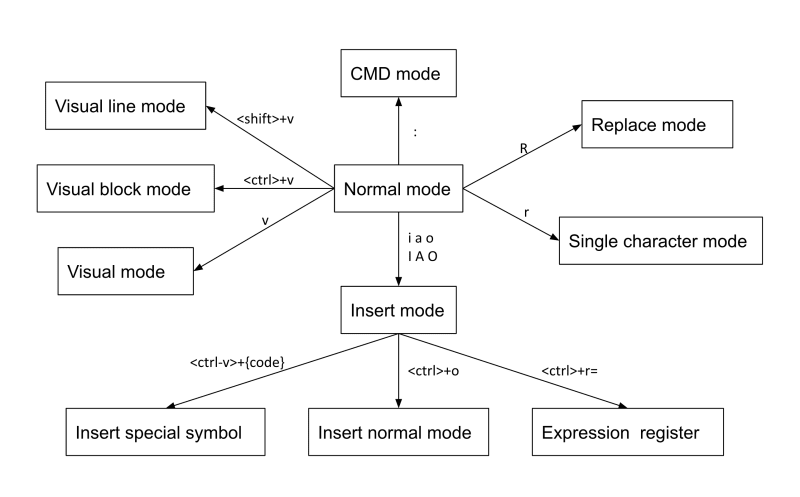
\includegraphics{images/png/vimmodes.png}
  \caption{Simplified Modes in Vim}
  \labfig{vimmodes}
\end{figure}

The figure \reffig{vimmodes} demonstrates how to switch between
the different modes in vim.
\sidenote{
  This is a simplified version of the modes in vim.
  There are other interim modes and other keystrokes
  that toggle the modes. This is shown in detail in
  \reffig{vim-modes}.
}

\begin{figure*}[h]
  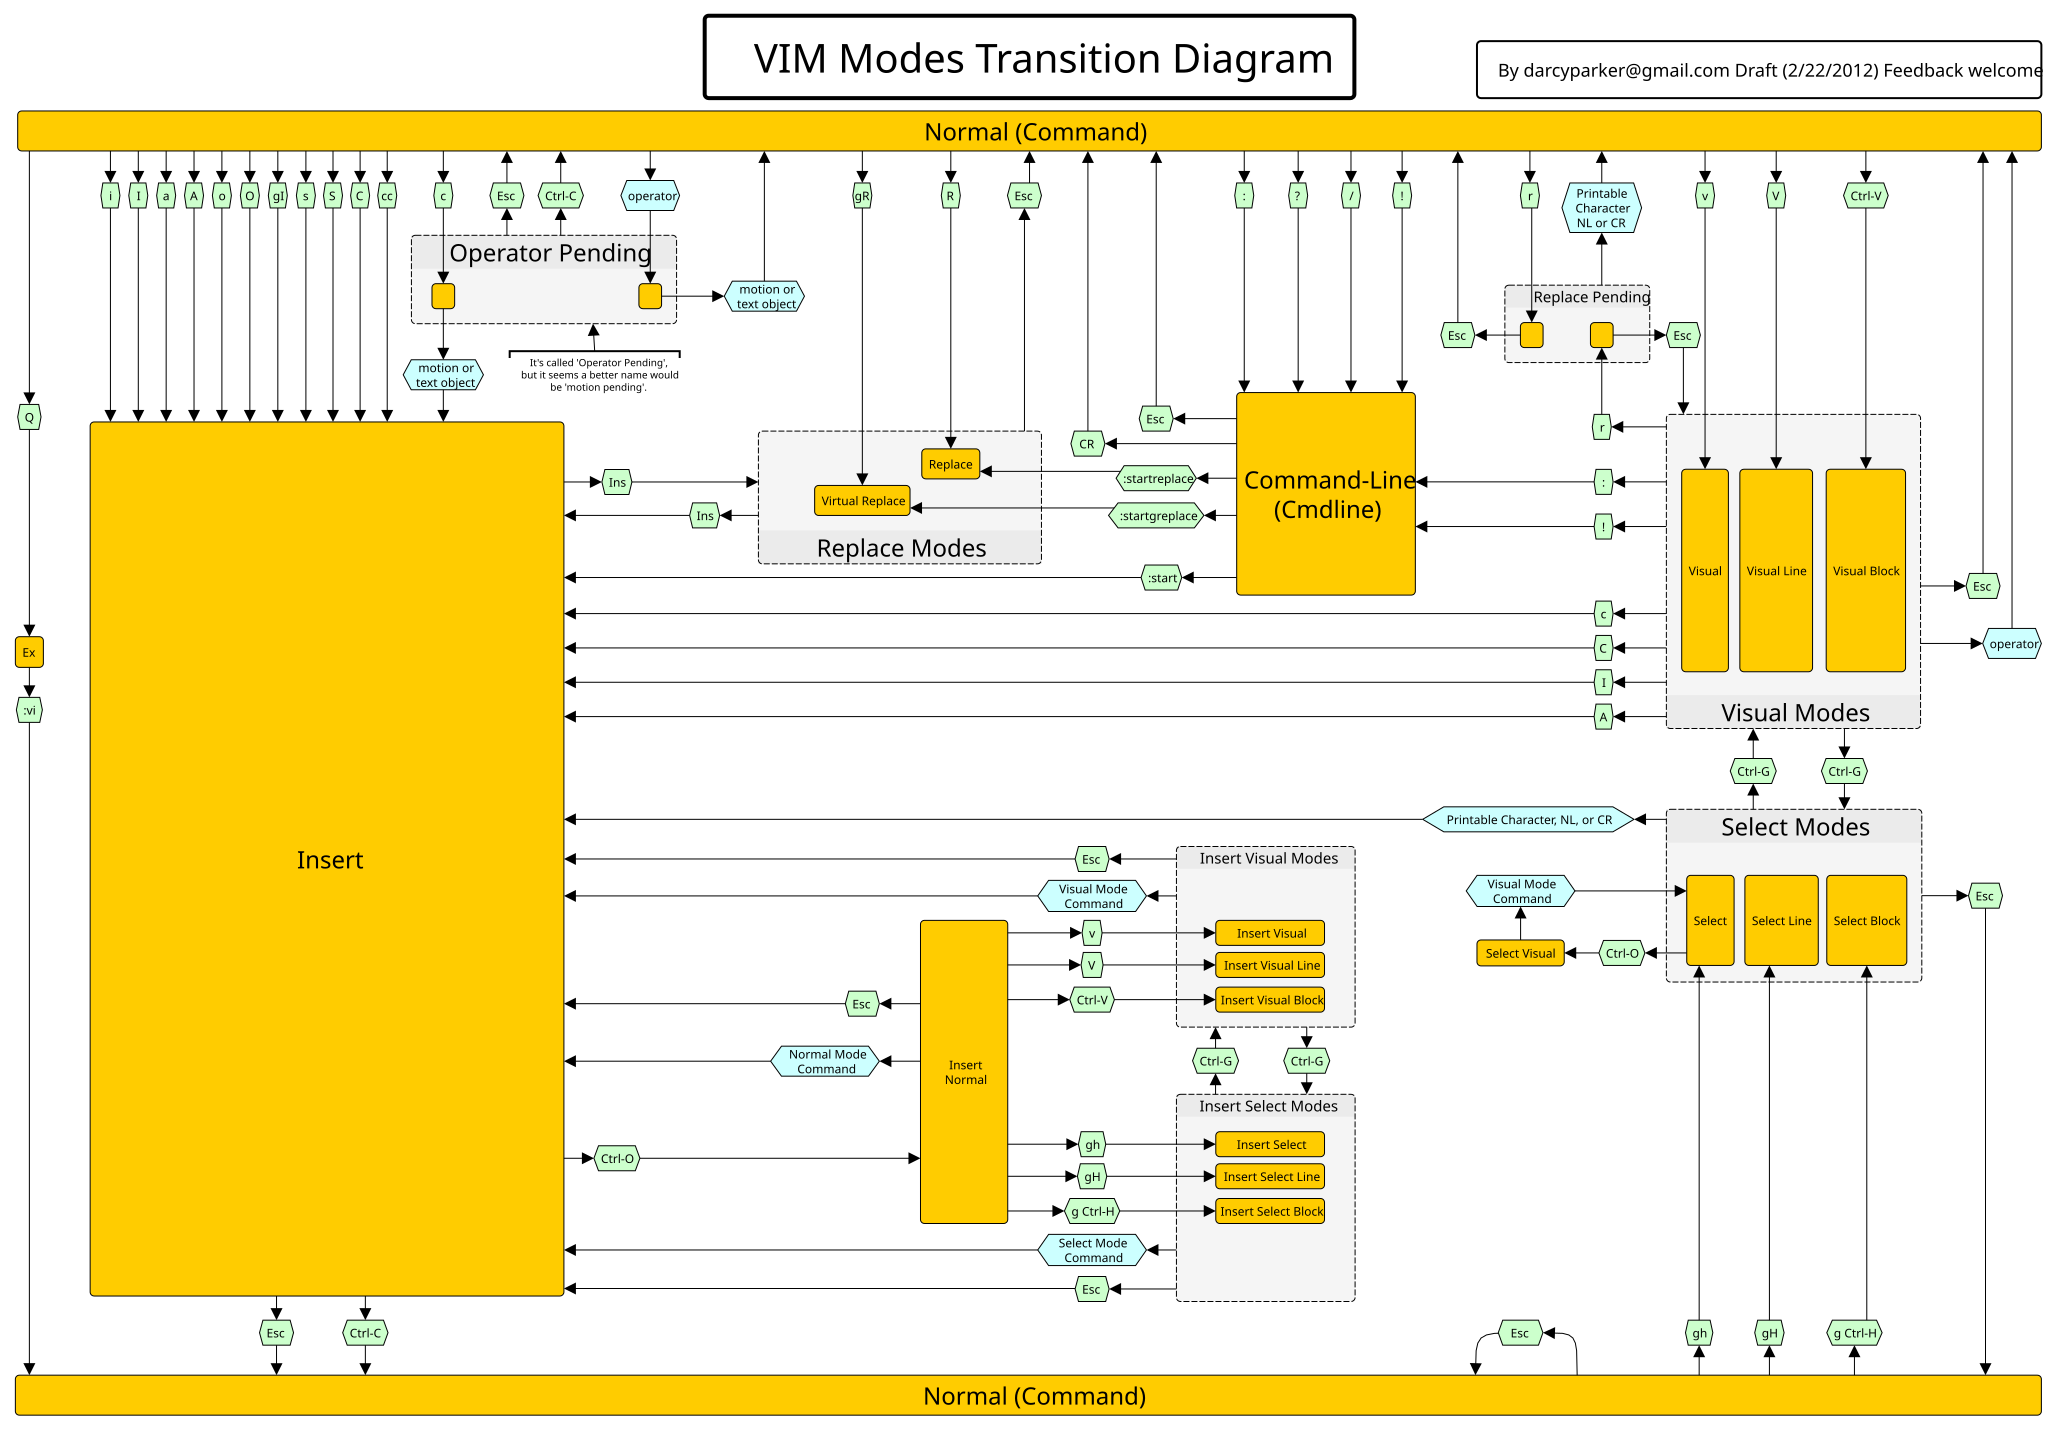
\includegraphics{images/png/vim-modes.png}
  \caption{Detailed Modes in Vim}
  \labfig{vim-modes}
\end{figure*}

\textbf{Commands in Ex mode}

Since we are already familar with commands in
\textbf{ed}, most of the commands are same/similar
in \textbf{ex} mode of vim.

\begin{table}[h!]
  \caption{Ex Commands in Vim}
  \labtab{ex-vim}
  \begin{tabular}{c l}
    \toprule
    Key & Description \\
    \midrule
    \texttt{:f} & show name of file \\
    \texttt{:p} & print current line \\
    \texttt{:a} & append at current line \\
    \texttt{:c} & change current line \\
    \texttt{:d} & delete current line \\
    \texttt{:i} & insert line at current position \\
    \texttt{:j} & join lines \\
    \texttt{:s} & search and replace regex pattern in current line \\
    \texttt{:m} & move current line to position \\
    \texttt{:u} & undo latest change \\
    \texttt{:w [filename]} & write buffer to filename \\
    \texttt{:q} & quit if no change \\
    \texttt{:wq} & write buffer to filename and quit \\
    \texttt{:x} & write buffer to filename and quit \\
    \texttt{:q!} & quit without saving \\
    \texttt{:r filename} & read file contents into buffer \\
    \texttt{:r !command} & read command output into buffer \\
    \texttt{:e filename} & edit a file \\
    \texttt{:sp [filename]} & split the screen and open another file \\
    \texttt{:vsp [filename]} & vertical split the screen and open another file \\
    \bottomrule
  \end{tabular}
\end{table}

There are many more commands in the ex mode of vim.
Along with implementing the original ed commands, it
also has a lot of additional commands to make it more
integrated with the vim editor, such as the ability
to open split windows, new tabs, buffers, and perform
normal mode commands in ex mode.

\textbf{Basic Navigation}

The basic keys for moving around in a text file in vim
are the \texttt{h,j,k,l} keys. They move the cursor
one character to the left, down, up, and right respectively.
These keys are chosen because they are present on the
home row of the keyboard, and do not require the user
to move their hands from the home row to navigate.
\sidenote{
  These were historically chosen because the ADM-3A terminal
  had these keys for navigation as seen in \reffig{adm3a}.
}

Along with these, we have keys to navigate word by word,
or to move to the next pattern match, or the next
paragraph, spelling error, etc.

\begin{table}[h!]
  \caption{Navigation Commands in Vim}
  \labtab{nav-vim}
  \begin{tabular}{c l}
    \toprule
    Key & Description \\
    \midrule
    \texttt{h} & move cursor left \\
    \texttt{j} & move cursor down \\
    \texttt{k} & move cursor up \\
    \texttt{l} & move cursor right \\
    \texttt{w} & move to the beginning of the next word \\
    \texttt{e} & move to the end of the current word \\
    \texttt{b} & move to the beginning of the previous word \\
    \texttt{\%} & move to the matching parenthesis, bracket, or brace \\
    \texttt{0} & move to the beginning of the current line \\
    \texttt{\$} & move to the end of the current line \\
    \texttt{/} & search forward for a pattern \\
    \texttt{?} & search backward for a pattern \\
    \texttt{n} & repeat the last search in the same direction \\
    \texttt{N} & repeat the last search in the opposite direction \\
    \texttt{gg} & move to the first line of the file \\
    \texttt{G} & move to the last line of the file \\
    \texttt{1G} & move to the first line of the file \\
    \texttt{1gg} & move to the first line of the file \\
    \texttt{:1} & move to the first line of the file \\
    \texttt{\{} & move to the beginning of the current paragraph \\
    \texttt{\}} & move to the end of the current paragraph \\
    \texttt{fg} & move cursor to next occurrence of `g' in the line \\
    \texttt{Fg} & move cursor to previous occurrence of `g' in the line \\
    \bottomrule
  \end{tabular}
\end{table}

\textbf{Wait you forgot your cursor behind!}

All of the above commands move the cursor to the
mentioned location. However, if you want to move
the entire screen, and keep the cursor at the
its current position, you can use the \texttt{z}
command along with \texttt{t} to top the line,
\texttt{b} to bottom the line, and \texttt{z} to
center the line.

There are other commands using the \texttt{Ctrl} key
that moves the screen, and not the cursor.

\begin{table}[h!]
  \caption{Moving the Screen Commands in Vim}
  \labtab{screen-vim}
  \begin{tabular}{c l}
    \toprule
    Key & Description \\
    \midrule
    \texttt{Ctrl+F} & move forward one full screen \\
    \texttt{Ctrl+B} & move backward one full screen \\
    \texttt{Ctrl+D} & move forward half a screen \\
    \texttt{Ctrl+U} & move backward half a screen \\
    \texttt{Ctrl+E} & move screen up one line \\
    \texttt{Ctrl+Y} & move screen down one line \\
    \bottomrule
  \end{tabular}
\end{table}

\textbf{Replacing Text}

Usually in other text editors, if you have a word, phrase, or line
which you want to replace with another, you would either press
the backspace or delete key to remove the text, and then type
the new text. However, in vim, there is a more efficient way
to replace text.

\begin{table}[h!]
  \caption{Replacing Text Commands in Vim}
  \labtab{replace-vim}
  \begin{tabular}{c l}
    \toprule
    Key & Description \\
    \midrule
    \texttt{r} & replace the character under the cursor \\
    \texttt{R} & replace the character from the cursor till escape is pressed \\
    \texttt{cw} & change the word under the cursor \\
    \texttt{c4w} & change the next 4 words \\
    \texttt{C} & delete from cursor till end of line and enter insert mode \\
    \texttt{cc} & delete entire line and enter insert mode \\
    \texttt{5cc} & delete next 5 lines and enter insert mode \\
    \texttt{S} & delete entire line and enter insert mode \\
    \texttt{s} & delete character under cursor and enter insert mode \\
    \bottomrule
  \end{tabular}
\end{table}

\textbf{Toggling Case}

You can toggle the case of a character, word, line,
or any arbitrary chunk of the file using the \texttt{~}
or the \texttt{g~} command.

\begin{table}[h!]
  \caption{Toggling Case Commands in Vim}
  \labtab{togglecase-vim}
  \begin{tabular}{c l}
    \toprule
    Key & Description \\
    \midrule
    \texttt{\textasciitilde} & toggle the case of the character under the cursor \\
    \texttt{g~w} & toggle the case of the word under the cursor \\
    \texttt{g~0} & toggle the case from cursor till beginning of line \\
    \texttt{g~\$} & toggle the case from cursor till end of line \\
    \texttt{g~\{} & toggle the case from cursor till previous empty line \\
    \texttt{g~\{} & toggle the case from cursor till next empty line \\
    \texttt{g~\%} & toggle the case from the bracket, brace, or parenthesis till its pair \\
    \bottomrule
  \end{tabular}
\end{table}

You might start to see a pattern emerging here.
Many commands in vim do a particular command,
and on which text it operates is determined by
the character followed by it. Such as \texttt{c}
to change, \texttt{d} to delete, \texttt{y} to yank,
etc. The text on which the command operates is
mentioned using \texttt{w} for the word, \texttt{0}
for till beginning of line, etc.

This is not a coincidence, but rather a design
of vim to make it more efficient to use.
The first command is called the operator command,
and the second command is called the motion command.

Vim follows a \texttt{operator-count-motion} pattern.
For example: \texttt{d2w} deletes the next 2 words.
This makes it very easy to learn and remember commands,
since you are literally typing out what you want to do.

\textbf{Deleting or Cutting Text}

In Vim, the delete command is used to cut text from the file.

\begin{table}[h!]
  \caption{Deleting Text Commands in Vim}
  \labtab{delete-vim}
  \begin{tabular}{c l}
    \toprule
    Key & Description \\
    \midrule
    \texttt{x} & delete the character under the cursor \\
    \texttt{X} & delete the character before the cursor \\
    \texttt{5x} & delete the next 5 characters \\
    \texttt{dw} & delete the word under the cursor \\
    \texttt{d4w} & delete the next 4 words \\
    \texttt{D} & delete from cursor till end of line \\
    \texttt{dd} & delete entire line \\
    \texttt{6dd} & delete next 6 lines \\
    \bottomrule
  \end{tabular}
\end{table}

\textbf{Motion - till, in, around}

By now you should notice that \texttt{dw} doesn't always
delete the word under the cursor. Technically \texttt{dw}
means delete till the beginning of the next word.
So if you press \texttt{dw} at the beginning of a word,
it will delete the word under the cursor. But if your
cursor is in the middle of a word and you type \texttt{dw},
it will only delete the part of the word till the beginning
of the next word from the cursor position.

To delete the entire word under the cursor, regardless of
where the cursor is in the word, you can use the \texttt{diw}
this means \textbf{d}elete \textbf{i}nside \textbf{w}ord.

However, now you may notice that \texttt{diw} doesn't delete
the space after the word. This results in two consequtive spaces,
one from the end of the word, and one from the beginning of the
word being left behind. To delete the space as well, you can use
\texttt{daw} which means \textbf{d}elete \textbf{a}round \textbf{w}ord.

This works not just with \texttt{w} but with any other motion
such as \textbf{d}elete \textbf{i}nside \textbf{p}aragraph,
which will delete the entire paragraph under the cursor,
resulting in two empty lines being left behind,
and \textbf{d}elete \textbf{a}round \textbf{p}aragraph,
which will delete the entire paragraph under the cursor,
and only one empty line being left behind.

Try out the same with deleting inside other items, such as
brackets, parenthesis, braces, quotes, etc. The syntax remains
the same, \texttt{di\{}, \texttt{di[}, \texttt{di(}, \texttt{di"}, \texttt{di'}, etc.

\textbf{Yanking and Pasting Text}

Yes, copying is called yanking in vim. The command to yank
is \texttt{y} and to paste is \texttt{p}.
You can combine \texttt{y} with all the motions and
\textbf{in} and \textbf{around} motions as earlier.
You can also add the count to yank multiple lines or words.

\begin{table}[h!]
  \caption{Deleting Text Commands in Vim}
  \labtab{delete-vim}
  \begin{tabular}{c l}
    \toprule
    Key & Description \\
    \midrule
    \texttt{yy} & yank the entire line \\
    \texttt{yw} & yank the word under the cursor \\
    \vdots & \vdots \\
    \texttt{p} & paste the yanked text after the cursor \\
    \texttt{P} & paste the yanked text before the cursor \\
    \bottomrule
  \end{tabular}
\end{table}

\begin{remark}
  Important to note that the commands
  \begin{lstlisting}
  yy \end{lstlisting}
  and
  \begin{lstlisting}
  0y$ \end{lstlisting}
  are not the same. The first command yanks the entire line,
  including the newline character at the end of the line.
  The second one yanks the entire line, but does not include
  the newline character at the end of the line.
  Thus if you directly press \texttt{p} after the first command,
  it will paste the line below the current line, and if you
  press \texttt{p} after the second command, it will paste
  the line at the end of the current line.
\end{remark}

\textbf{Undo and Redo}

The undo command in vim is \texttt{u} and the redo command
is \texttt{Ctrl+R}. You can undo multiple changes, unlike ed.

\begin{remark}
  If you want to use vim as your primary editor,
  it is highly recommended to install the
  \textbf{mbbill/undotree} plugin. This plugin
  will show you a tree of all the changes you
  have made in the current buffer, and you can
  go to any point in the tree and undo or redo
  changes. This becomes very useful if you undo
  too many changes and by mistake make a new change,
  this changes your branch in undo tree, and you cannot redo
  the changes you undid. With the undotree plugin,
  you can switch branches of the undo tree and redo
  the changes.
\end{remark}

\textbf{Searching and Replacing}

The search command in vim is \texttt{/} for forward search
and \texttt{?} for backward search. You can use the \texttt{n}
command to repeat the last search in the same direction,
and the \texttt{N} command to repeat the last search in the
opposite direction. For example, if you perform forward search
then using the \texttt{n} command will search for the next
occurrence of the pattern in the forward direction, and using
the \texttt{N} command will search for the previous occurrence
of the pattern in the backward direction. However if you perform
a backward search using the \texttt{?} command, then using the
\texttt{n} command will search for the previous occurrence of the
pattern in the backward direction, and using the \texttt{N} command
will search for the next occurrence of the pattern in the forward
direction.

You can also use the \texttt{*} command to search for the word
under the cursor, and the \texttt{\#} command to search for the
previous occurrence of the word under the cursor.

You can perform search and replace using the \texttt{:s} command.
The command takes a line address on which to perform the search
and replace. Usually you can use the \texttt{\%} address to
search in the entire file, or the \texttt{.,\$} address to
search from cursor till the end of the file.

You can also use any line number to specify the address range,
similar to the ed editor.

\begin{lstlisting}
:[addr]s/pattern/replace/[flags]
\end{lstlisting}

The flags at the end of the search and replace command can be
\textbf{g} to replace all occurrences in the line, and
\textbf{c} to confirm each replacement.

The address can be a single line number, a range of line numbers,
or a pattern to search for. The pattern can be a simple string,
or a regular expression.

Some examples of addresses are shown in \reftab{address-vim}.

\begin{table}[h!]
  \caption{Address Types in Search and Replace}
  \labtab{address-vim}
  \begin{tabular}{c l}
    \toprule
    Key & Description \\
    \midrule
    \texttt{m,n} & from line m to line n \\
    \texttt{m} & line m \\
    \texttt{m,\$} & from line m to end of file \\
    \texttt{.,\$} & from current line to end of file \\
    \texttt{1,n} & from line 1 to line n \\
    \texttt{/regex/,n} & from line containing regex to line n \\
    \texttt{m,/regex/} & from line m to line containing regex \\
    \texttt{.,/regex/} & from current line to line containing regex \\
    \texttt{/regex/,.} & from line containing regex to current line \\
    \texttt{1,/regex/} & from the first line to line containing regex \\
    \texttt{/regex/,\$} & from line containing regex to the last line \\
    \texttt{/regex1/;/regex2/} & from line containing regex1 to line containing regex2 \\
    \texttt{\%} & entire file \\
    \bottomrule
  \end{tabular}
\end{table}

\textbf{Insert Mode}

\begin{table}[h!]
  \caption{Keys to enter Insert Mode}
  \labtab{insert-vim}
  \begin{tabular}{c l}
    \toprule
    Key & Description \\
    \midrule
    \texttt{i} & enter insert mode before the cursor \\
    \texttt{a} & enter insert mode after the cursor \\
    \texttt{I} & enter insert mode at the beginning of the line \\
    \texttt{A} & enter insert mode at the end of the line \\
    \texttt{o} & add new line below the current line and enter insert mode \\
    \texttt{O} & add new line above the current line and enter insert mode \\
    \bottomrule
  \end{tabular}
\end{table}

You can enter insert mode from escape mode using the
keys listed in \reftab{insert-vim}.
In insert mode, if you want to insert any non-graphical character,
you can do that by pressing \texttt{Ctrl+V} followed by the
key combination for the character. For example, to insert
a newline character, you can press \texttt{Ctrl+V} followed
by \texttt{Enter}.

These are just the basic commands to get you started with vim.
You can refer to vim cheat sheets present online to get
more familiar with the commands.

\begin{itemize}
  \item \url{https://vim.rtorr.com/} is a good text based HTML cheat sheet for vim.
  \item \url{https://vimcheatsheet.com/} is a paid graphical cheat sheet for vim.
    \sidenote{
      A free version of the graphical cheat sheet is shown in \reffig{vimcheat}.
    }
\end{itemize}

\begin{figure*}[p]
  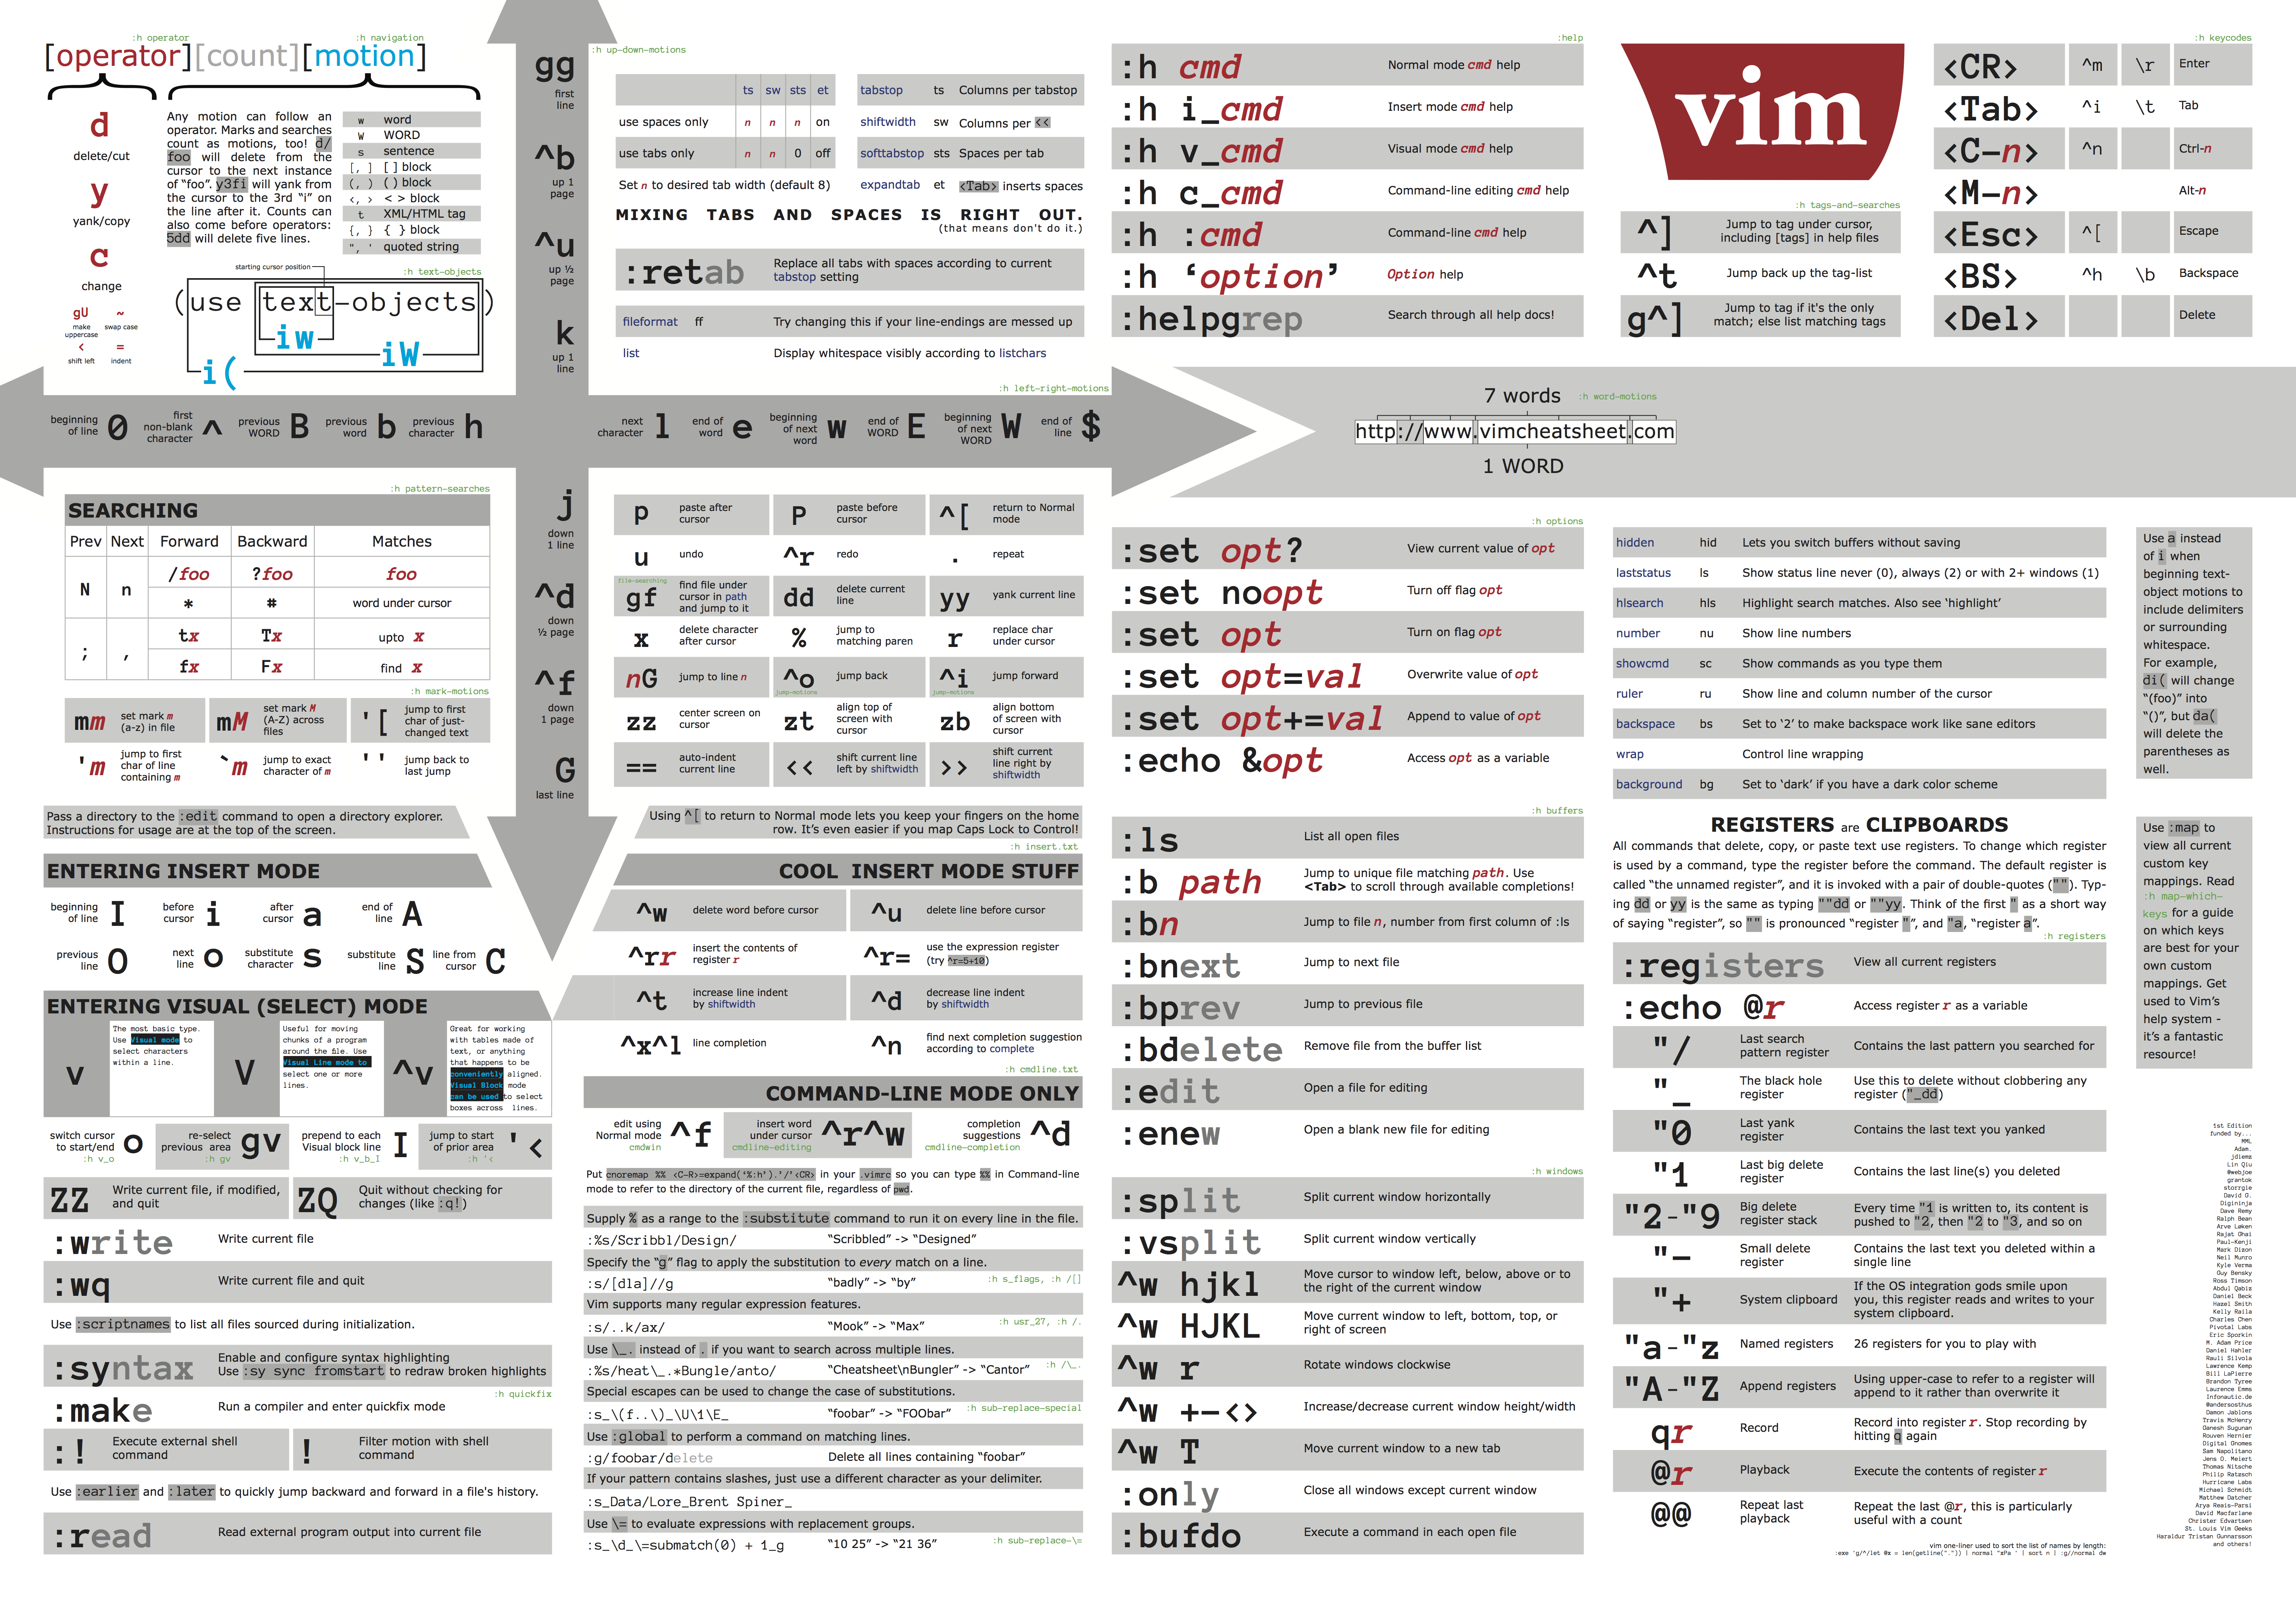
\includegraphics{images/png/vimcheat.png}
  \caption{Vim Cheat Sheet}
  \labfig{vimcheat}
\end{figure*}

\vfill
\pagebreak
\section{Emacs}

\subsection{History}

Emacs was mostly developed by Richard Stallman and Guy Steele.

\begin{table}[h!]
\caption{History of Emacs}
\labtab{emacshistory}
\centering
\begin{minipage}[t]{.7\linewidth}
\color{gray}
\rule{\linewidth}{1pt}
\ytl{1962}{TECO (Tape Editor and Corrector) was developed at MIT}
\ytl{1976}{Richard Stallman visits Stanford AI Lab and sees Fred Wright's E editor}
\ytl{1978}{Guy Steele accumulates a collection of TECO macros into EMACS}
\ytl{1979}{EMACS becomes MIT's standard text editor}
\ytl{1981}{James Gosling writes Gosling Emacs that runs on UNIX}
\ytl{1984}{Richard Stallman starts GNU Emacs - a free software alternative to Gosling Emacs}
\bigskip
\rule{\linewidth}{1pt}
\end{minipage}
\end{table}

\begin{marginfigure}[-8cm]
  
\includegraphics{images/png/emacs.png}
  \caption{Emacs Logo}
  \labfig{emacs}
\end{marginfigure}


\begin{marginfigure}
  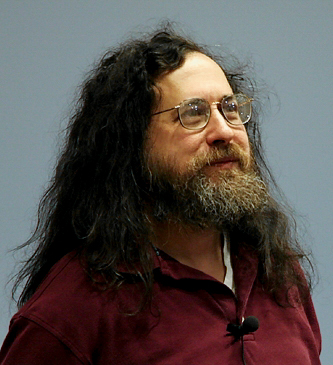
\includegraphics{images/png/stallman.png}
  \caption{Richard Stallman - founder of GNU and FSF projects}
  \labfig{stallman}
\end{marginfigure}

\textbf{TECO}

TECO was developed at MIT in 1962. It was a text editor
used to correct the output of the PDP-1 computer.
It is short for Tape Editor and Corrector.
Unlike most modern text editors,
TECO used separate modes in which the user would either
add text, edit existing text, or display the document
One could not place characters directly into a document
by typing them into TECO, but would instead enter a
character ('i') in the TECO command language telling
it to switch to input mode, enter the required characters,
during which time the edited text was not displayed on
the screen, and finally enter a character (<esc>) to
switch the editor back to command mode. This is very
similar to how vi works.

\textbf{Stallman's Visit to Stanford}

In 1976, Richard Stallman visited the Stanford AI Lab
where he saw Fred Wright's E editor. He was impressed
by E's WYSIWYG
\sidenote{
  What You See Is What You Get
}
interface where you do not need to tackle multiple
modes to edit a text file. This is the default behaviour
of most modern editors now.
He then returned to MIT where he found that
Carl Mikkelsen had added to TECO a combined
display/editing mode called Control-R that allowed
the screen display to be updated each time the user
entered a keystroke. Stallman reimplemented this mode
to run efficiently and added a macro feature to the TECO
display-editing mode that allowed the user to redefine
any keystroke to run a TECO program.

Initially TECO was able to only edit the file
sequentially, page by page. This was due to earlier
memory restrictions of the PDP-1.
Stallman modified TECO to read the entire file into
the buffer, and then edit the buffer in memory
allowing for random access to the file.

\textbf{Too Many Macros!}

The new version of TECO quickly became popular at
the AI Lab and soon accumulated a large collection
of custom macros whose names often ended in MAC or
MACS, which stood for macro.
This quickly got out of hand as there were many
divergent macros, and a user would be totally
lost when using a co-worker's terminal.

\begin{marginfigure}
  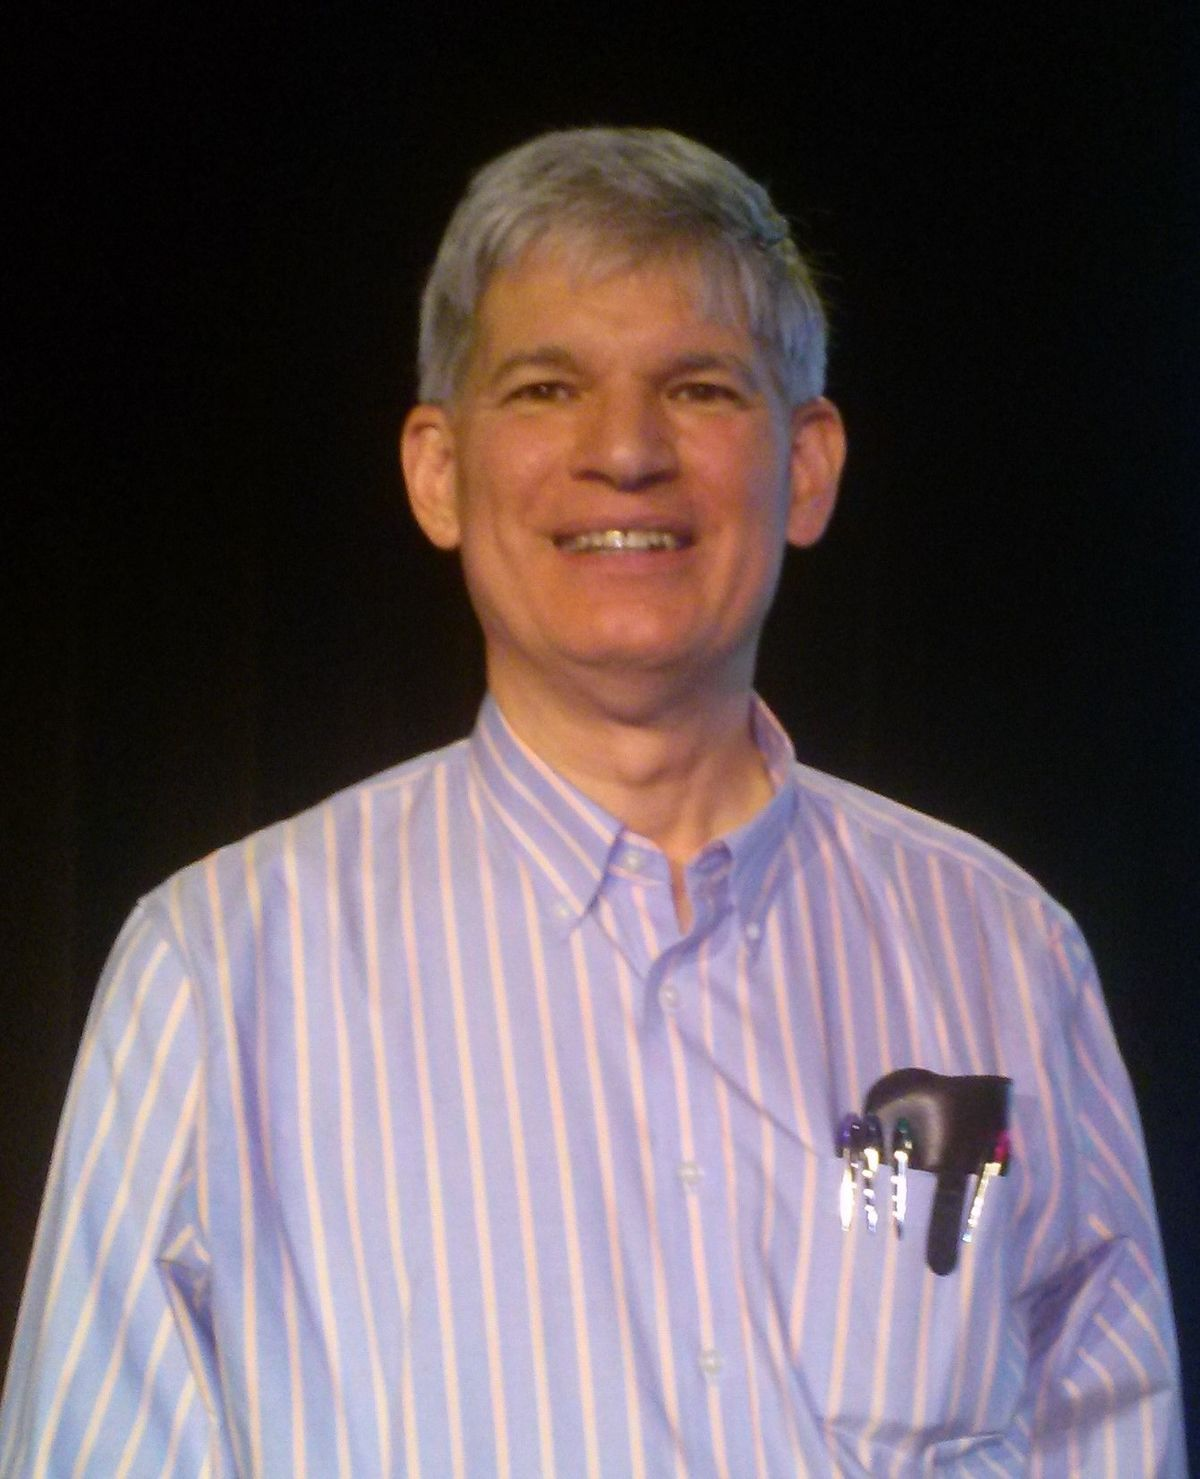
\includegraphics{images/png/steele.png}
  \caption{Guy L. Steele Jr. combined many divergent TECO with macros to create EMACS}
  \labfig{steele}
\end{marginfigure}


In 1979, Guy Steele combined many of the popular
macros into a single file, which he called EMACS,
which stood for Editing MACroS, or E with MACroS.

To prevent thousands of forks of EMACS, Stallman
declared that
`EMACS was distributed on a basis of communal sharing,
which means all improvements must be given back to me
to be incorporated and distributed.'

Till now, the EMACS, like TECO, ran on the PDP-10
which ran the ITS operating system and not UNIX.

\textbf{EINE ZWEI SINE and other clones}

No, that is not German.
These are some of the popular clones of EMACS
made for other operating systems.

EINE
\sidenote{
  EINE stands for Eine Is Not EMACS
}
was a text editor developed in the late 1970s.
In terms of features, its goal was to `do what Stallman's
PDP-10 (original) Emacs does'.
Unlike the original TECO-based Emacs, but like Multics Emacs,
EINE was written in Lisp. It used Lisp Machine Lisp.

In the 1980s, EINE was developed into ZWEI
\sidenote{
  ZWEI stands for ZWEI Was Eine Initially
}.
Innovations included programmability in Lisp Machine Lisp,
and a new and more flexible doubly linked
list method of internally representing buffers.

\marginnote{
  These kinds of recursive acronyms are common in the
  \*nix world. For example, GNU stands for GNU's Not Unix,
  WINE (A compatibility layer to run Windows applications)
  is short for WINE Is Not an Emulator.
}

SINE
\sidenote{
  SINE stands for SINE Is Not EINE
}
was written by Owen Theodore Anderson in 1981.

In 1978, Bernard Greenberg wrote a version of EMACS
for the Multics operating system called Multics EMACS.
This used Multics Lisp.


\begin{marginfigure}
  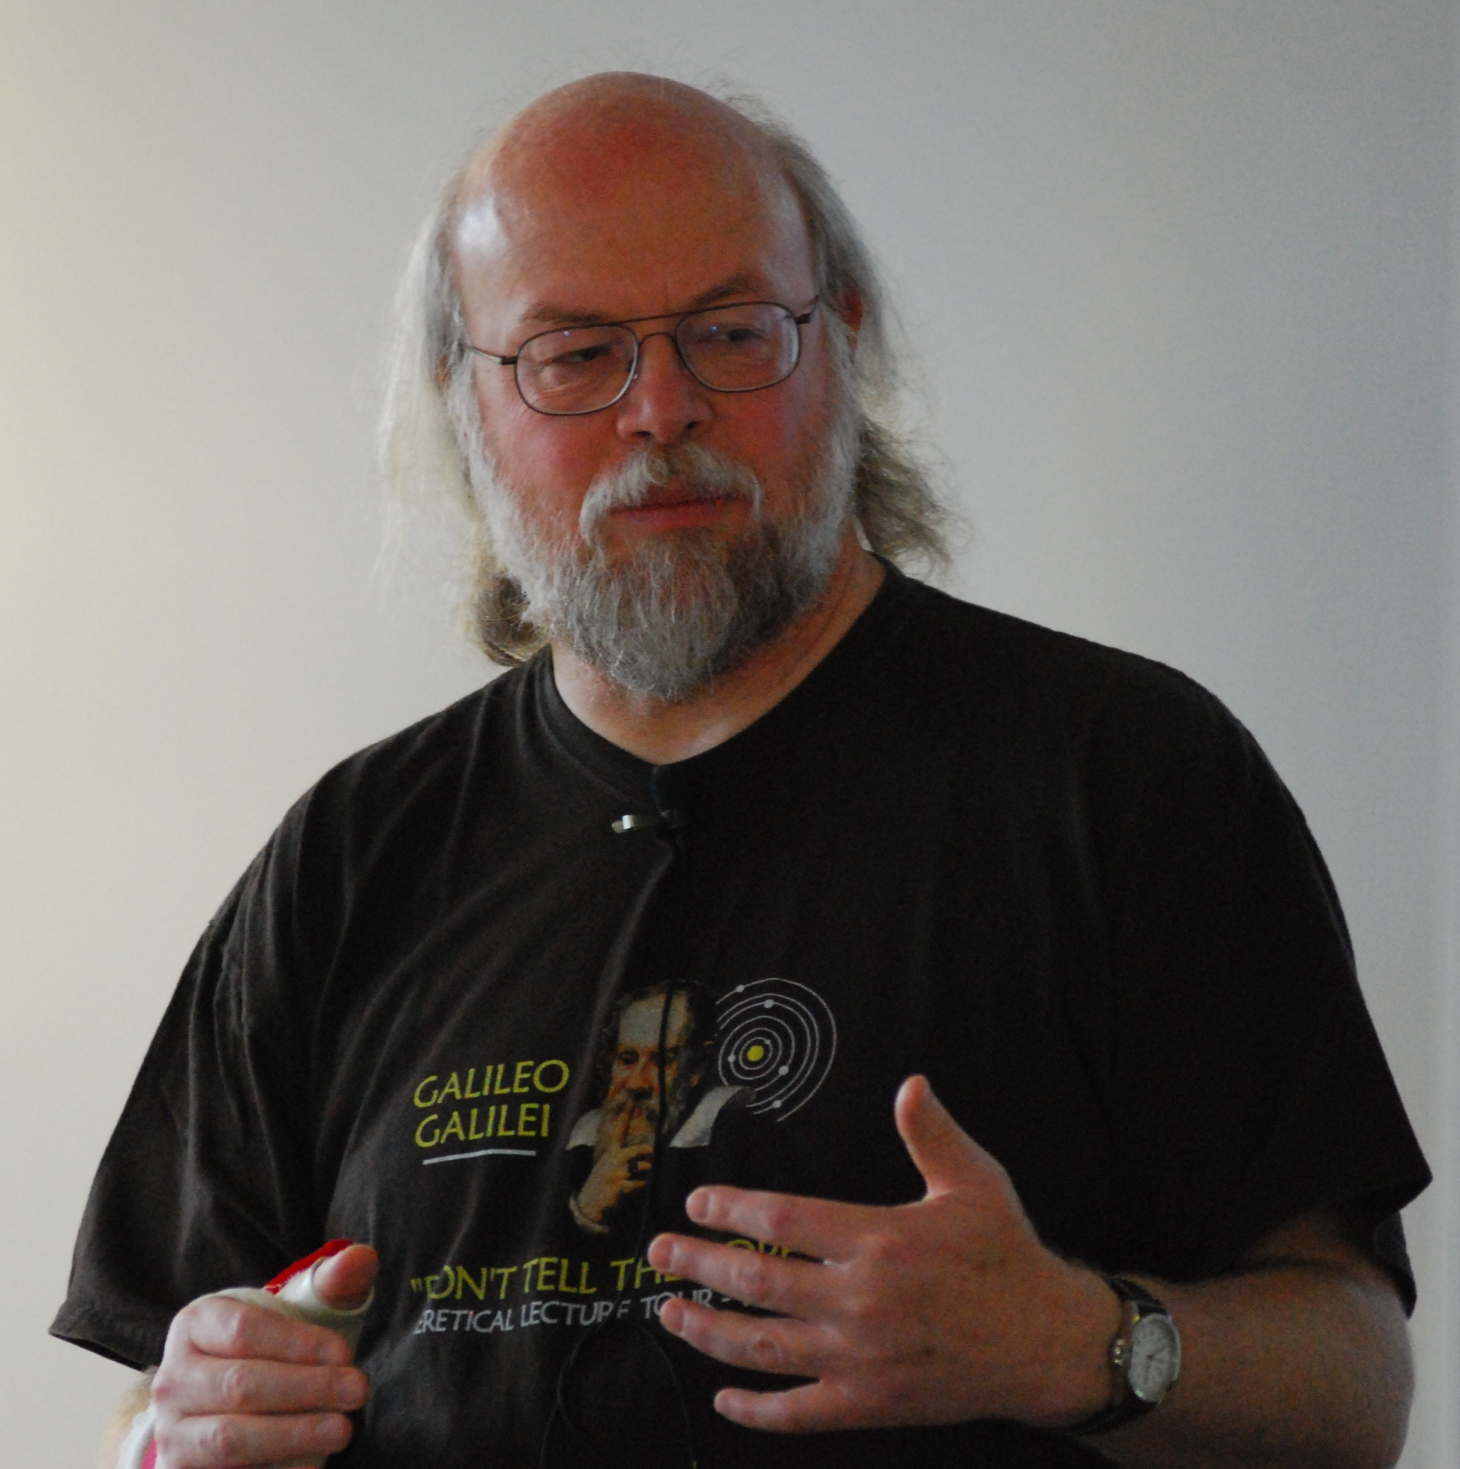
\includegraphics{images/png/gosling.png}
  \caption{James Gosling - creator of Gosling Emacs and later Java}
  \labfig{gosling}
\end{marginfigure}

\textbf{Gosling Emacs}

In 1981, James Gosling wrote Gosling Emacs for UNIX.
It was written in C and used Mocklisp, a language with
lisp-like syntax, but not a lisp. It was not free software.

\textbf{GNU Emacs}

In 1983, Stallman started the GNU project to create a
free software alternatives to proprietary softwares
and ultimately to create a free
\sidenote{
Recall from the previous chapter that free software
does not mean a software provided gratis, but a software
which respects the user's freedom to run, copy, distribute,
and modify the software. It is like free speech, not free beer.
}
operating system.

In 1984, Stallman started GNU Emacs, a free software
alternative to Gosling Emacs. It was written in C and
used a true Lisp dialect, Emacs Lisp as the extension
language. Emacs Lisp was also implemented in C.
This is the version of Emacs that is most popular today
and available on most operating systems repositories.

\textbf{How the developer's keyboard influences the editors they make}

Remember that ed was made while using \textbf{ADM-3A}
which looked like \reffig{adm3a-real}.

\begin{marginfigure}
  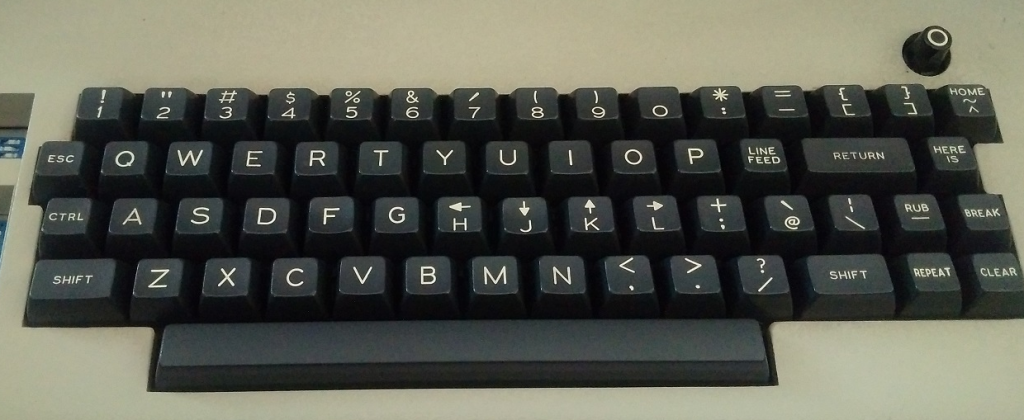
\includegraphics{images/png/adm3a-real.png}
  \caption{ADM-3A terminal}
  \labfig{adm3a-real}
\end{marginfigure}

Whereas emacs was made while the \textbf{Knight keyboard}
and the \textbf{Space Cadet keyboard} were in use, which
can be seen in \reffig{space-cadet}.

\begin{marginfigure}
  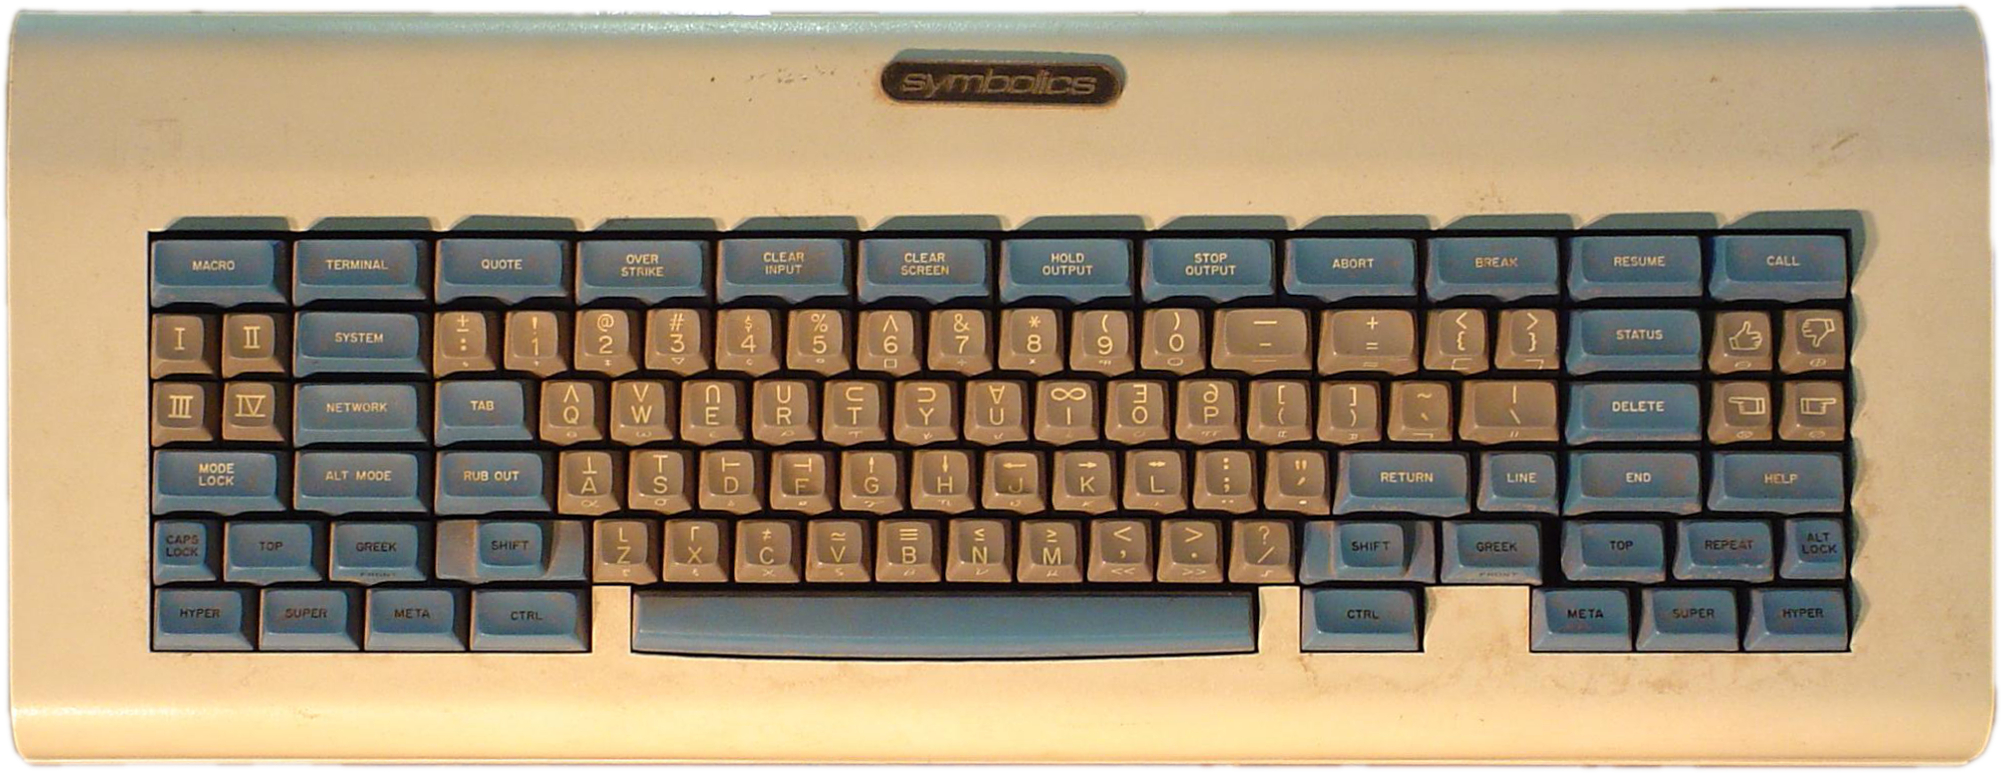
\includegraphics{images/png/space-cadet.png}
  \caption{Space Cadet Keyboard}
  \labfig{space-cadet}
\end{marginfigure}

Notice how the ADM-3A has very limited modifier keys, and
does not even have arrow keys. Instead it uses \texttt{h,j,k,l}
keys as arrow keys with a modifier. This is why vi uses
mostly key combinations and a modal interface.
Vi also uses the \texttt{Esc} key to switch between modes,
which is present conveniently in place of the Caps Lock or Tab key
in modern keyboard layouts.

The Space Cadet keyboard has many modifier keys, and even
a key for the Meta key. This is why emacs uses many key
modifier combinations, and has a lot of keybindings.

\subsection{Exploring Emacs}

This is not a complete overview of Emacs, or even its
keybindings. A more detailed reference card can be
found on their
\href{https://www.gnu.org/software/emacs/refcards/pdf/refcard.pdf}{website}.

\textbf{Opening a File}

We can open a file in emacs by providing its
filename as an argument to the emacs executable.

\begin{lstlisting}[language=bash]
$ emacs test.txt
\end{lstlisting}

Most of emacs keybindings use modifier keys such as
the \texttt{Ctrl} key, and the \texttt{Meta} key.
The \texttt{Meta} key is usually the \texttt{Alt} key
in modern keyboards. In the reference manual and here,
we will be representing the \texttt{Meta} key as \texttt{M-}
and the \texttt{Ctrl} key as \texttt{C-}.

\textbf{Basic Navigation}

These keys are used to move around in the file.
Like vim, emacs also focusses on keeping the hands
free from the mouse, and on the keyboard.
All the navigation can be done through the keyboard.

\begin{table}[h!]
  \caption{Navigation Commands in Emacs}
  \labtab{nav-emacs}
  \begin{tabular}{c l}
    \toprule
    Key & Description \\
    \midrule
    \texttt{C-p} & move up one line \\
    \texttt{C-b} & move left one char \\
    \texttt{C-f} & move right one char \\
    \texttt{C-n} & move down one line \\
    \texttt{C-a} & goto beginning of current line \\
    \texttt{C-e} & goto end of current line \\
    \texttt{C-v} & move forward one screen \\
    \texttt{M-<} & move to first line of the file \\
    \texttt{M-b} & move left to previous word \\
    \texttt{M-f} & move right to next word \\
    \texttt{M->} & move to last line of the file \\
    \texttt{M-a} & move to beginning of current sentence \\
    \texttt{M-e} & move to end of current sentence \\
    \texttt{M-v} & move back one screen \\
    \bottomrule
  \end{tabular}
\end{table}

\textbf{Exiting Emacs}

We can exit emacs either with or without saving the file.
We can also suspend emacs and return to the shell.
This is a keymapping of the shell, and not of emacs.

\begin{table}[h!]
  \caption{Exiting Emacs Commands}
  \labtab{exit-emacs}
  \begin{tabular}{c l}
    \toprule
    Key & Description \\
    \midrule
    \texttt{C-x C-s} & save buffer to file \\
    \texttt{C-z} & suspend emacs \\
    \texttt{C-x C-c} & exit emacs and stop it \\
    \bottomrule
  \end{tabular}
\end{table}

\textbf{Searching Text}

Emacs can search for a fixed string, or a regular expression
and replace it with another string.

\begin{table}[h!]
  \caption{Searching Text Commands in Emacs}
  \labtab{search-emacs}
  \begin{tabular}{c l}
    \toprule
    Key & Description \\
    \midrule
    \texttt{C-s} & search forward \\
    \texttt{C-r} & search backward \\
    \texttt{M-x} & replace string \\
    \bottomrule
  \end{tabular}
\end{table}

\textbf{Copying and Pasting}

Copying can done by marking the region, and then copying it.

\begin{table}[h!]
  \caption{Copying and Pasting Commands in Emacs}
  \labtab{copy-emacs}
  \begin{tabular}{c l}
    \toprule
    Key & Description \\
    \midrule
    \texttt{M-backspace} & cut the word before cursor \\
    \texttt{M-d} & cut the word after cursor \\
    \texttt{M-w} & copy the region \\
    \texttt{C-w} & cut the region \\
    \texttt{C-y} & paste the region \\
    \texttt{C-k} & cut from cursor to end of line \\
    \texttt{M-k} & cut from cursor to end of sentence \\
    \bottomrule
  \end{tabular}
\end{table}

\vfill
\pagebreak
\section{Nano}

\begin{marginfigure}
  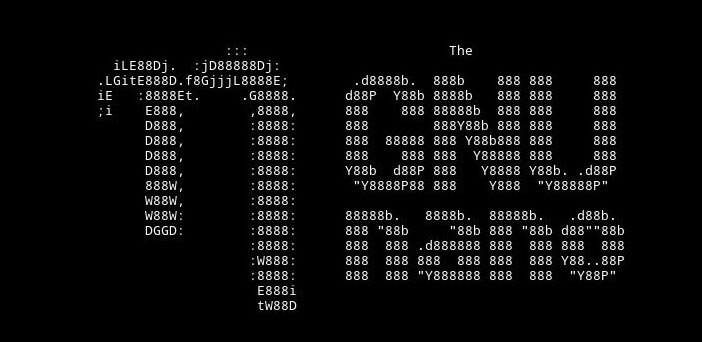
\includegraphics{images/png/nano.png}
  \caption{Nano Text Editor}
  \labfig{nano}
\end{marginfigure}

Although vim and emacs are the most popular
command line text editors, nano is also a very
useful text editor for beginners. It is very
simple and does not have a steep learning curve.

It is a non-modal text editor, which means that
it does not have different modes for different
actions. You can directly start typing text
as soon as you open \textbf{nano}.

Although it uses modifier keys to invoke commands,
it does not have a lot of commands as vim or emacs.

\subsection{History}

Pine
\sidenote{
  It is believed that pine stands for
  Pine is Not Elm, Elm being another
  text-based email client.
  However, the author clarifies that
  it was not named with that in mind.
  Although if a backronym was to be made,
  he prefered `Pine is Nearly Elm' or
  `Pine is No-longer Elm'
}
was a text-based email client developed at the
University of Washington. It was created in 1989.
The email client also had a text editor built in
called Pico.

Although the license of Pine and Pico may seem
open source, it was not. The license was restrictive
and did not allow for modification or redistribution.
\sidenote{
Up to version 3.91, the Pine license was similar to BSD, and it stated that
`Permission to use, copy, modify, and distribute this software and its documentation for any purpose and without fee to the University of Washington is hereby granted ...'
The university registered a trademark for the Pine name with respect to `computer programs used in communication and electronic mail applications' in March 1995.
From version 3.92, the holder of the copyright, the University of Washington, changed the license so that even if the source code was still available, they did not allow modifications and changes to Pine to be distributed by anyone other than themselves. They also claimed that even the old license never allowed distribution of modified versions.
}

Due to this, many people created clones of Pico
with free software licenses. One of the most popular
clones was TIP (TIP isn't Pico) which was created by
Chris Allegretta in 1999. Later in 2000 the name was
changed to Nano.
\sidenote{
  Mathematically, nano is $10^{-9}$ or one billionth.
  and pico is $10^{-12}$ or one trillionth.
  or put relatively, nano is 1000 times bigger than pico,
  although the size of nano binary is smaller than pico.
}
In 2001, nano became part of the GNU project.

GNU nano implements several features that Pico lacks,
including syntax highlighting, line numbers,
regular expression search and replace,
line-by-line scrolling, multiple buffers,
indenting groups of lines, rebindable key support,
and the undoing and redoing of edit changes.

In most modern linux systems, the \textbf{nano}
binary is present along with the \textbf{pico}
binary, which is actually a symbolic link to the
\textbf{nano} binary.

You can explore this by finding the path of the
executable using the \texttt{which} command
and long-listing the executable.

\begin{lstlisting}[language=bash]
$ which pico
/usr/bin/pico
$ ls -l /usr/bin/pico
lrwxrwxrwx 1 root root 22 Sep  6  2023 /usr/bin/pico -> /etc/alternatives/pico
$ ls -l /etc/alternatives/pico
lrwxrwxrwx 1 root root 9 Sep  6  2023 /etc/alternatives/pico -> /bin/nano
\end{lstlisting}

\begin{remark}
  Note that here we have a symlink to another symlink.
  Theoretically, you can extend to as many levels of
  chained symlinks as you want.
  Thus, to find the final sink of the symlink chain,
  you can use the \texttt{readlink -f} command or
  the \texttt{realpath} command.
\end{remark}

\begin{lstlisting}[language=bash]
$ realpath $(which pico)
/usr/bin/nano
\end{lstlisting}

\subsection{Exploring Nano}

In nano, the Control key is represented by the \textasciicircum symbol.
The Meta or Alt key is represented by the \texttt{M-}.

\textbf{File Handling}

You can open a file in nano by providing the filename
as an argument to the nano executable.

\begin{lstlisting}[language=bash]
$ nano test.txt
\end{lstlisting}

\begin{table}[h!]
  \caption{File Handling Commands in Nano}
  \labtab{file-nano}
  \begin{tabular}{c l}
    \toprule
    Key & Description \\
    \midrule
    \texttt{\textasciicircum S} & save the file \\
    \texttt{\textasciicircum O} & save the file with a new name \\
    \texttt{\textasciicircum X} & exit nano \\
    \bottomrule
  \end{tabular}
\end{table}

\textbf{Editing}

Nano is a simple editor, and you can do without learning
any more commands than the ones listed above, but here
are some more basic commands for editing text.

\begin{table}[h!]
  \caption{Editing Commands in Nano}
  \labtab{edit-nano}
  \begin{tabular}{c l}
    \toprule
    Key & Description \\
    \midrule
    \texttt{\textasciicircum K} & cut current line and save in cutbuffer \\
    \texttt{M-6} & copy current line and save in cutbuffer \\
    \texttt{\textasciicircum U} & paste contents of cutbuffer \\
    \texttt{M-T} & cut until end of buffer \\
    \texttt{\textasciicircum ]} & complete current word \\
    \texttt{M-U} & undo last action \\
    \texttt{M-E} & redo last undone action \\
    \texttt{\textasciicircum J} & justify the current paragraph \\
    \texttt{M-J} & justify the entire file \\
    \texttt{M-:} & start/stop recording a macro \\
    \texttt{M-;} & run the last recorded macro \\
    \texttt{F12} & invoke the spell checker, if available \\
    \bottomrule
  \end{tabular}
\end{table}

There are many more commands in nano, but they are
omitted from here for brevity. You can find the
complete list of keybindings by pressing \texttt{\textasciicircum G}
key in nano, or by running \lstinline[language=bash]{info nano}.
\marginnote{
  You can also find third-party cheat sheets
  \href{https://www.cheatsheet.wtf/Nano/}{online}.
}

\subsection{Editing A Script in Nano}

Since learning nano is mostly to be able to edit
a text file even if you are not familiar with
either vim or emacs, let us try to edit a simple
script file to confirm that you can use nano.

\begin{lstlisting}[language=bash]
$ touch myscript.sh
$ chmod u+x myscript.sh
$ nano myscript.sh
\end{lstlisting}

Now try to write a simple script in the file.
An example script is shown below.

\begin{lstlisting}[language=bash]
#!/bin/bash
read -rp 'What is your name? ' name
echo "Hello $name"
date=$(date "+%H:%M on a %A")
echo "Currently it is $date"
\end{lstlisting}

\marginnote{
  If you do not understand how the script works,
  do not worry. It will be covered in depth in
  later chapters.
}

Now save the file by pressing \texttt{\textasciicircum S}
\begin{remark}
  In some systems, the \texttt{\textasciicircum S} key
  will freeze the terminal. Any key you press after this
  will seem to not have any effect.
  This is because it is interpreted as the \texttt{XOFF}
  and is used to lock the scrolling of the terminal.
  To unfreeze the terminal, press \texttt{\textasciicircum Q}.
  In such a system, you can save the file by pressing
  \texttt{\textasciicircum O} and then typing out the
  name of the file if not present already, and pressing
  Enter.
  To disable this behaviour, you can add the line
  \begin{lstlisting}[language=bash]
  set -ixon \end{lstlisting}
  to your \texttt{.bashrc} file.
\end{remark}
and exit nano by pressing \texttt{\textasciicircum X}.

Now you can run the script by typing

\begin{lstlisting}[language=bash]
$ ./myscript.sh
What is your name? Sayan
Hello Sayan
Currently it is 21:50 on a Tuesday
\end{lstlisting}

Now that we are able to edit a text file using text editors,
we are ready to write scripts to solve problems.

% \setchapterpreamble[u]{\margintoc}
\chapter{Networking and SSH}
\labch{ssh}


\section{Networking}

\subsection{What is networking?}

Have you ever tried to get some work done on a computer
while the internet was down? It's a nightmare.
Modern day computing relies highly on networking.
But what is networking?

\begin{definition}[Networking]
A computer network comprises two or more computers
that are connected—either by cables (wired) or wifi
(wireless)—with the purpose of transmitting, exchanging,
or sharing data and resources.
\end{definition}

We have been using the computer, and linux, for a while now
but the utility of a computer increases exponentially when
it is connected to a network. It allows computers to share
files and resources, and to communicate with each other.
Current day world wide web is built on the internet.

\begin{definition}[Internet]
Internet is a global network of networks that connects
millions of computers worldwide. It allows computers to
connect to other computers across the world through a
hierarchy of routers and servers.
\end{definition}

Learning about networking and how networking works
is useful, although we won't be devling into details
in this book. It is left as an exercise for the reader
to explore external resources if they are interested.

\marginnote{
One succinct blogpost explaining how the internet works
from which the figure \reffig{networks} is taken
is available at
\url{https://www.highspeedinternet.com/resources/how-the-internet-works}
}

\subsection{Types of Networks}

\begin{marginfigure}
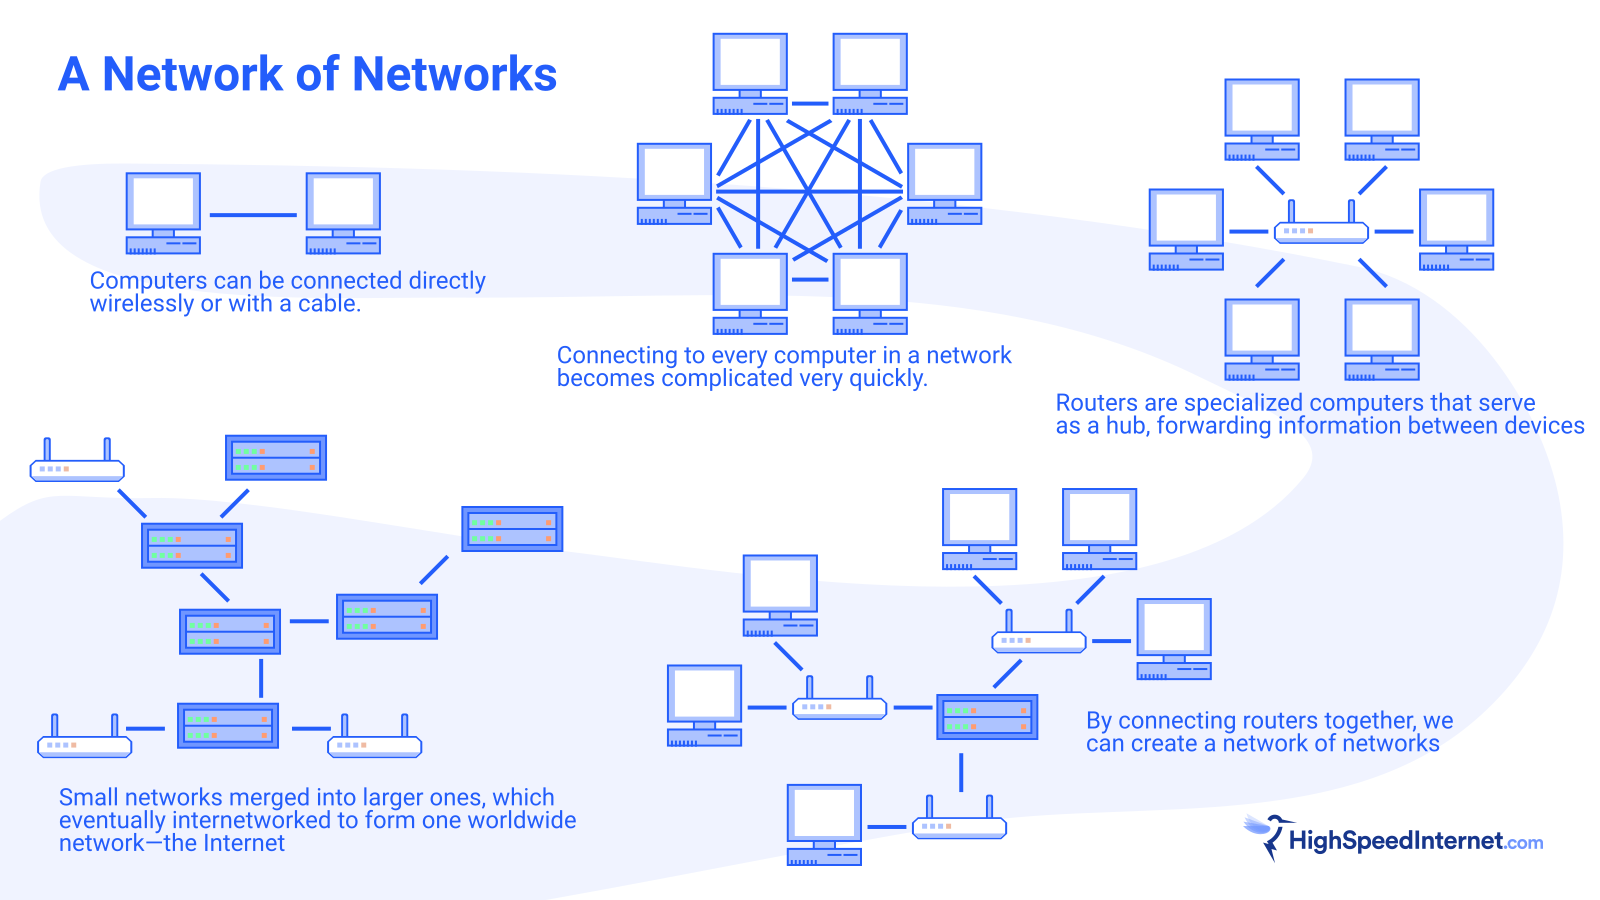
\includegraphics{networks}
\caption{Types of Networks}
\labfig{networks}
\end{marginfigure}

If the end goal is to connect computers with each other,
one naive solution might be to connect all the computers
with each other. Although this might seem intuitive at
first, this quickly gets out of hand when the number of
computers keep increasing.

If we have $n$ computers, then the number of connections
required to connect all the computers with each other
is given by the formula

\[
\frac{n(n-1)}{2} = \frac{n^2 - n}{2}
\]

This is a quadratic function and grows very quickly.

\begin{marginfigure}
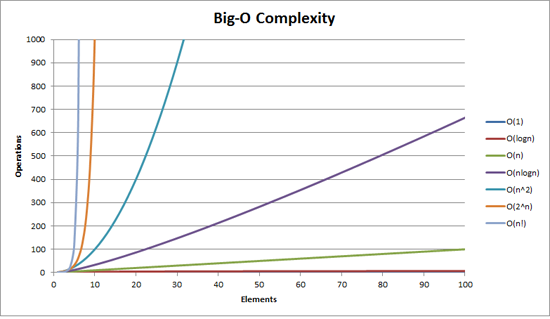
\includegraphics{complexity}
\caption{Growth Rate of Different Functions - Note how quickly $n^2$ grows}
\labfig{complexity}
\end{marginfigure}

This means it will cost a lot to connect all the computers
to each other. This is applicable not only in computer
networking with physical wires, but in many other fields.
Take an examples of airlines and airplane routes. If there
were $n$ airports, then the number of routes required to
connect all the airports is given by the same formula.
This would be disastrous for the economy and the environment
if we ran so many airplanes daily. So what gives?

\textbf{Hub and Spoke Network}

\begin{marginfigure}
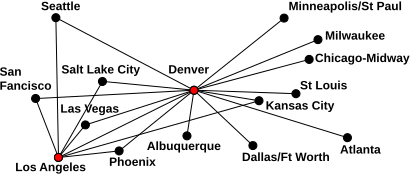
\includegraphics{airlines}
\caption{Hub and Spoke Model Employed by Airlines}
\labfig{airlines}
\end{marginfigure}

The solution to this problem is to use a hub and spoke
model, where there are one, or multiple, central hubs
which connect to many other nodes. Any path from any
node to another goes through one or more hubs. This
reduces the number of connections required to connect
all the nodes.

This is the solution used in airlines, and also in
most computer networks.
\sidenote{
  Although computer networks use a hub model
  for the local area network, the network of
  networks, especially the gateway routers
  follow a mesh model to ensure redundancy
  and make the network more robust.
}

Due to this, networks can be classified into three
broad categories based on their geographical area
coverage.

\begin{marginfigure}
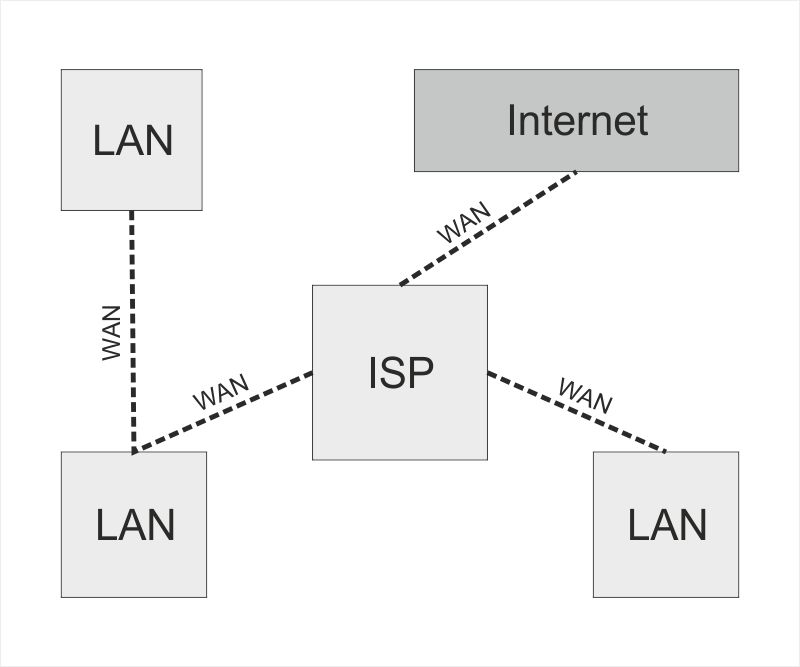
\includegraphics{wan}
\caption{LAN and WAN connecting to the Internet}
\labfig{wan}
\end{marginfigure}

\begin{itemize}
\item \textbf{Local Area Network (LAN)}: A network
that covers a small geographical area, like a
home, office, or a building.
\item \textbf{Metropolitan Area Network (MAN)}:
A network that covers a larger geographical area,
like a city or a town.
\item \textbf{Wide Area Network (WAN)}: A network
that covers a large geographical area, like a
country or the entire world.
\end{itemize}

To connect these networks to computers and also
to each other, we require some special devices.

\subsection{Devices in a Network}

In computer networks, this hub of the
Hub and Spoke Model can either be a
level 1 hub, a level 2 switch, or a level 3 router.

\textbf{Hub}

A hub will simply broadcast the message to all
the connected nodes. This causes a lot of traffic
to be generated and is not very efficient. Hub does
not have the capability to identify which node
is who. This is called a level 1 hub.
\sidenote{
  To understand more about the levels, refer
  \href{https://en.wikipedia.org/wiki/OSI\_model}{OSI Model}
}

\textbf{Switch}

A switch is smarter than a hub. It can identify
each device connected to it and can send the
packets of data only to the intended recipient.
This is more efficient than a hub. This is called
a level 2 switch since it uses the level 2 of the
OSI model (Data Link Layer) to identify the devices.
This means that the devices are identified by their
MAC addresses.
Using this, you can only communicate with devices
in your local network. This is useful for a home
network or a office network. But we cannot communicate
with the entire world using this, since it doesn't
understand IP addresses.

\textbf{Router}

\begin{marginfigure}
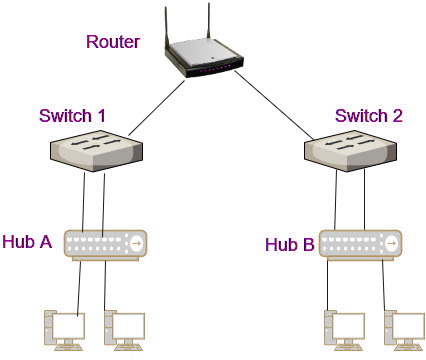
\includegraphics{hsr}
\caption{Hub, Switch, Router connecting to the Internet}
\labfig{hsr}
\end{marginfigure}

A router is even smarter than a switch. It can
understand IP addresses and can route the packets
from one network to another. This is called a level 3
router since it uses the level 3 of the OSI model
(Network Layer) to identify the devices. This means
that the networks are identified by their IP addresses.
This is what we use to connect to the internet.
The internet is nothing but a whole lot of routers
communicating with each other to find the optimal
path to send the packets to its destination.
Border Gateway Protocol (BGP) is the protocol used
by routers to communicate with each other and find
the optimal path. They usually are connected in a
mesh network to ensure redundancy and robustness.

\textbf{Level 3 Switch}

A level 3 switch, or a routing switch, is a switch
with the capabilities of a router. It can understand
the language of IP addresses and can route the packets
to different networks. This is useful in large
organizations where there are many networks and
each network can be divided into subnetworks called
VLANs.

\marginnote{
  You can read more about the differences between
  these devices
  \href{https://www.cbtnuggets.com/blog/technology/networking/l1-l2-vs-l3-whats-the-difference}{online}.
}

So, in short, internet is a network of network
of \dots networks. It is a hierarchical structure
connecting all the computers in the world.
Some computers are connected earlier in the
hierarchy (usually the ones closer geographically)
and some are connected later.

\subsection{IP Addresses}

So how do routers know which where to send the
data packets? This is where IP addresses come in.
To communicate over the internet, two computers
need to know their public IP addresses. The routers
then finds the optimal path to send the data packets
to the destination network.

IP addresses are of two types: IPv4 and IPv6.
The most common one is IPv4, which is a 32-bit
address represented as four octets separated by
dots. For example,

\[
162.136.73.21
\]

Here, each octet can take values from 0 to 255.
\sidenote{
  An octet is a group of 8 bits. Since an IP
  address is 32 bits, it is represented as 4
  groups of 8 bits.
  8 bits can only represent numbers from 0 to 255.
  since $2^8 = 256$.
}
Technically all such combinations are possible
IP addresses, resulting in
$2^{32} = 4,294,967,296$ possible IP addresses.
That is a lot of IP addresses, but not enough
for the growing number of devices in the world.

This is where IPv6 comes in. IPv6 is a 128-bit
address represented as 8 groups of 4 hexadecimal
digits separated by colons. For example,

\[
2001:0db8:85a3:0000:0000:8a2e:0370:7334
\]

\marginnote{
  Notice that there are some groups of zeros
  in the address. These can be compressed by
  writing only one zero in place of multiple
  zeros in each group. Further, any leading
  zeros can be omitted for each group.
  Making the above address as
  \texttt{2001:db8:85a3:0:0:8a2e:370:7334}.
  Further, if there are multiple groups of zeros,
  they can be compressed to \texttt{::}.
  This can be used only once in an address.
  Doing this, the above address can be compressed
  further to
  \texttt{2001:db8:85a3::8a2e:370:7334}.
}

This results in
$2^{128} = 340282366920938463463374607431768211456$
possible IP addresses, which is a lot more than
IPv4.

\subsection{Subnetting}

\textbf{Legacy Classes}

\[
10.125.42.62 \rightarrow 0 0 0 0 1 0 1 0 . 0 1 1 1 1 1 0 1 . 0 0 1 0 1 0 1 0 . 0 0 1 1 1 1 1 0
\]

Recall that an IP address, although represented as
four octets, is actually a 32-bit address. This
means that in binary form, an IP address is a
string of 32 1s and 0s. Using the first four bits,
we can classify an IP address into five classes.

\begin{itemize}
\item \textbf{Class A}: The first bit is `0`. The
IP addresses in the range 0.0.0.0 to 127.255.255.255.
\item \textbf{Class B}: The first two bits are `10`.
IP addresses in the range 128.0.0.0 to 191.255.255.255.
\item \textbf{Class C}: The first three bits are `110`.
IP addresses in the range 192.0.0.0 to 223.255.255.255.
\item \textbf{Class D}: The first four bits are `1110`.
IP addresses in the range 224.0.0.0 to 239.255.255.255.
These are reserved for multicast addresses.
\item \textbf{Class E}: The first four bits are `1111`.
IP addresses in the range 240.0.0.0 to 255.255.255.255.
These are reserved for experimental purposes.
\end{itemize}

However, these classes do not simply assign an IP to
each machine. They are further divided into the
network part and the host part.

Class A assigns the first octet to the network part,
this is used to identify which network the machine
is in. The remaining three octets are used to identify
the host in that network. This means that a class A
network can have $2^{24} - 2 = 16,777,214$ hosts.
However, there can only be $2^{7} = 128$ class A
networks. Thus, class A networks are used by large
organizations which have many hosts, but not many
large organizations exist, so 128 networks are enough.

Similarly, class B assigns the first two octets to
identify the network and the remaining two octets
to identify the host. This means that a class B
network can have $2^{16} - 2 = 65,534$ hosts.
And there can be $2^{14} = 16,384$ class B networks.
These are used by medium-sized organizations, which
are plenty in number, and have a moderate number of
hosts.

The same goes for class C networks, where the first
three octets are used to identify the network and
the last octet is used to identify the host. This
network can have $2^{8} - 2 = 254$ hosts. And there
can be $2^{21} = 2,097,152$ class C networks. These
are used by small organizations, which are plenty
in number, and have a small number of hosts.

\textbf{Subnet Masks}

\begin{definition}[Subnetting]
The process of dividing a network into smaller network
sections is called subnetting.
\end{definition}

Usually, each network has only one subnet, which
contains all the hosts in that network. However,
the network can be further divided into smaller
subnetworks, each containing a subset of the hosts.
This is useful in large organizations where the
network is divided into departments, and each
department is given a subnetwork.

To indicate which part of the IP address is the
network part and which part is the host part, we
use a subnet mask. A subnet mask is a 32-bit
number where the first $n$ bits are 1s and the
remaining bits are 0s. The number of 1s in the
subnet mask indicates the number of bits used
to identify the network. For example, for the
IP Address \texttt{192.168.0.15}, it can be
written in binary as
\[
1100 0000 - 1010 1000 - 0000 0000 - 0000 1111
\]

As we know, it belongs to the class C network,
where the first three octets are used to identify
the network, and the rest is used to identify the
host. So the default network mask is

\[
1111 1111 - 1111 1111 - 1111 1111 - 0000 0000
\]

or \texttt{255.255.255.0} in decimal.
The network portion of the IP address is
found by taking the bitwise AND
\sidenote{
  The bitwise AND operation is a binary operation
  that takes two equal-length binary representations
  and performs the logical AND operation on each pair
  of corresponding bits. The result in each position
  is 1 if the first bit is 1 and the second bit is 1;
  otherwise, the result is 0.
}
of the IP address and the subnet mask.
This results in the network address
\[
1100 0000 - 1010 1000 - 0000 0000 - 0000 0000
\]
which is \texttt{192.168.0.0} and the host address
is \texttt{0000 1111} which is $15$.

However, if we do not require all the 8 bits in the
host space
\sidenote{
  That is, if we have less than 254 hosts in the
  network.
}
then we can use some of the initial bits of the
host space to identify subnetworks. This is called
subnetting.

For example, the netmask of \texttt{255.255.255.0}
leaves 8 bits for the host space, or $2^8 - 2 = 254$
\sidenote{
  We subtract 2 from the total number of hosts
  to account for the network address and the
  broadcast address, which are the first(0)
  and the last(255) addresses in the network.
}
hosts. If we want to split this network into
two subnets, we can use the MSB of the host space
for representing the subnetworks. This results in
each subnet having $2^7 - 2 = 126$ hosts.

\begin{remark}
Observe that we effectively lost two available addresses
from the total number of hosts in the network.
Earlier we could have $254$ hosts, but now we can
have only $126 \times 2 = 252$ hosts. This is because
each subnet also reserves the first and the last
address for the network address and the broadcast
address.
\end{remark}

To do this, we change the subnet mask to
\[
1111 1111 - 1111 1111 - 1111 1111 - 1000 0000
\]
which can be represented as \texttt{255.255.255.128}.

This gives us two subnets, one with the address range
of \texttt{192.168.0.1} to \texttt{192.168.0.127}, and
another of \texttt{192.168.0.129} to \texttt{192.168.0.255}.

\subsection{Private and Public IP Addresses}

But what if we want to communicate with computers
in our local network? This is where private IP
comes in. Some ranges of IP addresses are reserved
for private networks. These are not routable over
the internet. Each LAN has a private IP address
range, and the router translates these private
addresses to the public IP address when sending
the packets over the internet. The assignment
of these private IP addresses is done by the
DHCP server
\sidenote{
  Dynamic Host Configuration Protocol (DHCP) is
  a network management protocol used on Internet
  Protocol networks whereby a DHCP server dynamically
  assigns an IP address and other network configuration
  parameters to each device on a network so they can
  communicate with other IP networks.
}
in the router.

Each class of networks has a range of IP addresses
that are reserved for private networks.

\begin{table*}[h!]
\caption{Private IP Address Ranges}
\labtab{privateip}
\begin{tabular}{c c c c}
\toprule
Class & Network Bits (CIDR) & Address Range & Number of Addresses \\
\midrule
\textbf{Class A} & 8 & \texttt{10.0.0.0} - \texttt{10.255.255.255} & 16,777,216 \\
\textbf{Class B} & 12 & \texttt{172.16.0.0} - \texttt{172.31.255.255} & 1,048,576 \\
\textbf{Class C} & 16 & \texttt{192.168.0.0} - \texttt{192.168.255.255} & 65,536 \\
\bottomrule
\end{tabular}
\end{table*}

\subsection{CIDR}

However, this practice of subdividing IP addresses
into classes is a legacy concept, and not followed
anymore. Instead, we use CIDR (Classless Inter-Domain
Routing) to announce how many bits are used to identify
the network and how many bits are used to identify the
host.

For example, we could express the idea that the IP address
\texttt{192.168.0.15} is associated with the netmask
\texttt{255.255.255.0} by using the CIDR notation of
\texttt{192.168.0.15/24}. This means that the first
$24$ bits of the IP address given are considered
significant for the network routing.

This is helpful because not all organizations fit
into the tight categorization of the legacy classes.

\subsection{Ports}

Ports usually refer to physical holes in a computer
where you can connect a cable. However, in networking,
ports refer to logical endpoints for communication.

\begin{definition}[Port]
A port or port number is a number assigned to uniquely identify
a connection endpoint and to direct data to a specific service.
At the software level, within an operating system, a port is a
logical construct that identifies a specific process or a type
of network service.
\end{definition}

For any communication between two computers, the data
needs to be sent to a specific port. This is because
there are multiple services running on a computer, and
the operating system needs to know which service to
direct the data to.

There are $2^{16} = 65,536$ ports available for use.
However, the first $1024$ ports are reserved for
well-known services. These are called the \textbf{well-known
ports} and are used by services like HTTP, FTP, SSH, etc.
The well known ports can be found in \reftab{wellknownports}.

Other ports, from $1024$ to $49151$, are registered ports,
these ports can be registered with the Internet Assigned
Numbers Authority (IANA) by anyone who wants to use them
for a specific service.

Ports from $49152$ to $65535$ are dynamic ports, these
are used by the operating system for temporary connections
and are not registered.

Whenever you send a request to a web server for example,
the request is sent to the server's IP address and the
port number \texttt{80} which is the default port for
HTTP
\sidenote{
  or \texttt{443} for HTTPS.
}
but the port number from your (the client) side is
usually a random port number from the dynamic port range.
This is a short-lived port number and is used to
establish a connection with the server.

These kinds of ports which are short-lived and used
to establish a connection are called \textbf{ephemeral ports}.

\begin{table*}[h!]
\caption{Well-known Ports}
\labtab{wellknownports}
\begin{tabular}{c l c}
\toprule
Port Number & Service & Protocol \\
\midrule
20 & File Transfer Protocol (FTP) Data Transfer & TCP \\
21 & File Transfer Protocol (FTP) Command Control & TCP \\
22 & Secure Shell (SSH) Secure Login & TCP \\
23 & Telnet remote login service, unencrypted text messages & TCP \\
25 & Simple Mail Transfer Protocol (SMTP) email delivery & TCP \\
53 & Domain Name System (DNS) service & TCP/UDP \\
67, 68 & Dynamic Host Configuration Protocol (DHCP) & UDP \\
80 & Hypertext Transfer Protocol (HTTP) used in the World Wide Web & TCP \\
110 & Post Office Protocol (POP3) & TCP \\
119 & Network News Transfer Protocol (NNTP) & TCP \\
123 & Network Time Protocol (NTP) & UDP \\
143 & Internet Message Access Protocol (IMAP) Management of digital mail & TCP \\
161 & Simple Network Management Protocol (SNMP) & UDP \\
194 & Internet Relay Chat (IRC) & TCP \\
443 & HTTP Secure (HTTPS) HTTP over TLS/SSL & TCP \\
546, 547 & DHCPv6 IPv6 version of DHCP & UDP \\
\bottomrule
\end{tabular}
\end{table*}

\subsection{Protocols}

\begin{definition}[Protocols]
In computing, a protocol is a set of rules that define
how data is transmitted between devices in a network.
\end{definition}

There are many protocols used in networking, some of
the most common ones are

\begin{itemize}
    \item \textbf{HTTP}: HyperText Transfer Protocol
    \item \textbf{HTTPS}: HyperText Transfer Protocol Secure
    \item \textbf{FTP}: File Transfer Protocol
    \item \textbf{SSH}: Secure Shell
    \item \textbf{SMTP}: Simple Mail Transfer Protocol
    \item \textbf{POP3}: Post Office Protocol
    \item \textbf{IMAP}: Internet Message Access Protocol
    \item \textbf{DNS}: Domain Name System
    \item \textbf{DHCP}: Dynamic Host Configuration Protocol
    \item \textbf{NTP}: Network Time Protocol
    \item \textbf{SNMP}: Simple Network Management Protocol
    \item \textbf{IRC}: Internet Relay Chat
    \item \textbf{BGP}: Border Gateway Protocol
    \item \textbf{TCP}: Transmission Control Protocol
    \item \textbf{UDP}: User Datagram Protocol
\end{itemize}

These protocols act on the different layers of the
OSI model. For example, HTTP, HTTPS, FTP, SSH, etc.
are application layer protocols, while TCP, UDP, etc.
are transport layer protocols.

\subsection{Firewalls}

\begin{definition}[Firewall]
  A firewall is a network security system that monitors
  and controls incoming and outgoing network traffic
  based on predetermined security rules.
\end{definition}

A fireewall acts as a barrier between your computer
and the internet. It monitors the incoming and outgoing
traffic and blocks any traffic that does not meet the
security rules. This is useful to prevent unauthorized
access to your computer and to prevent malware from
entering your computer and/or communicating with the
outside world.

\begin{lstlisting}[language=bash]
$ sudo ufw enable # Enable the firewall
$ sudo ufw allow 22 # Allow SSH
$ sudo ufw allow 80 # Allow HTTP
$ sudo ufw allow 443 # Allow HTTPS
$ sudo ufw status # Check the status of the firewall
\end{lstlisting}

\subsection{SELinux}

We can have additional security by using SELinux
in addition to the firewall. SELinux is a security
module that provides access control security policies.
SELinux is short for Security-Enhanced Linux.
It provides a flexible Mandatory Access Control (MAC)
that restricts the access of users and processes to
files and directories.

\textbf{Least Privilege Principle}

\begin{definition}[Least Privilege Principle]
The principle of least privilege (POLP) is an important
concept in computer security, promoting minimal user
profile privileges on computers based on users' job
necessity.
\end{definition}

This principle states that a user should have only
the minimum privileges required to perform their job.
This principle is applied throughout linux, and also
in SELinux.

You can check if \textbf{SELinux} is enabled by running

\begin{lstlisting}[language=bash]
$ sestatus
\end{lstlisting}

If SELinux is enabled, you can check the context of
a file or a directory using

\begin{lstlisting}[language=bash]
$ ls -lZ
\end{lstlisting}

However, if SELinux is not enabled, it will show
a \texttt{?} in the context.

If SELinux is enabled, you can set the context of a
file or a directory using the \texttt{chcon} command.

\textbf{RBAC Items}

\begin{definition}[Role-Based Access Control (RBAC)]
Role-Based Access Control (RBAC) is a policy-neutral
access control mechanism defined around roles and
privileges. The components of RBAC such as role-permissions,
user-role, and role-role relationships make it simple
to perform user assignments.
\end{definition}

SELinux uses the concept of RBAC to control the access
of users and processes to files and directories.

There are four components in the SELinux context
that are used to control the access of users and
processes to files and directories, as shown in
\reffig{selinux}.

\begin{figure}[h!]
  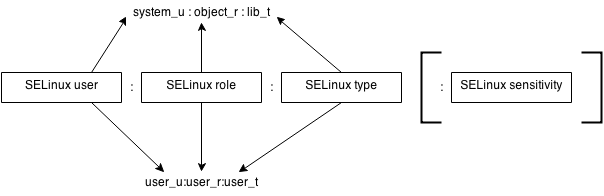
\includegraphics{selinux}
  \caption{SELinux Context}
  \labfig{selinux}
\end{figure}

\begin{itemize}
  \item \textbf{User}: The user who is trying to access
    the file or directory.
  \item \textbf{Role}: The role of the user, which defines
    the permissions of the user.
  \item \textbf{Type}: The type of the file or directory.
  \item \textbf{Domain}: The domain
    \sidenote{or type or sensitivity}
    of the process trying to access the file or directory.
\end{itemize}

\textbf{Modes of SELinux}

\begin{itemize}
  \item \textbf{Enforcing}: In this mode, SELinux is enabled
    and actively enforcing the security policies.
  \item \textbf{Permissive}: In this mode, SELinux is enabled
    but not enforcing the security policies. It logs the
    violations but does not block them.
  \item \textbf{Disabled}: In this mode, SELinux is disabled
    and not enforcing any security policies.
\end{itemize}

You can change the mode of SELinux by editing the
\texttt{/etc/selinux/config} file.

\begin{lstlisting}[language=bash]
$ sudo vim /etc/selinux/config
\end{lstlisting}

\textbf{Tools for SELinux}

\begin{itemize}
  \item \textbf{sestatus}: Check the status of SELinux.
  \item \textbf{semamange}: Manage the SELinux policy.
  \item \textbf{restorecon}: Restore the context of files
    and directories.
\end{itemize}


\subsection{Network Tools}

There are a lot of tools in GNU/Linux used for managing,
configuring, and troubleshooting networks. Some of the
important tools are listed in \reftab{networktools}.

\begin{table*}[h!]
  \caption{Network Tools}
  \labtab{networktools}
  \begin{tabular}{c l}
    \toprule
    \textbf{Tool} & \textbf{Description} \\
    \midrule
    \texttt{ip} & Show / manipulate routing, devices, policy routing and tunnels \\
    \texttt{ping} & To see if the remote machine is up \\
    \texttt{traceroute} & Diagnostics the hop timings to the remote machine \\
    \texttt{nslookup} & Ask for conversion of IP address to name \\
    \texttt{dig} & DNS lookup utility \\
    \texttt{netstat} & Print network connections \\
    \href{https://mxtoolbox.com/}{mxtoolbox} & Public accessibility of your server \\
    \href{https://whois.com/}{whois} & Information about the domain \\
    \texttt{nmap} & Network port scanner \\
    \texttt{wireshark} & Network protocol analyzer and packet sniffer \\
    \bottomrule
  \end{tabular}
\end{table*}

\textbf{ip}

To find out the private IP address of the NICs of your system,
you can run the \texttt{ip addr} command.
\sidenote{
  \texttt{ip a} also works.
}

\begin{lstlisting}[language=bash]
$ ip addr
1: lo: <LOOPBACK,UP,LOWER_UP> mtu 65536 qdisc noqueue state UNKNOWN group default qlen 1000
    link/loopback 00:00:00:00:00:00 brd 00:00:00:00:00:00
    inet 127.0.0.1/8 scope host lo
       valid_lft forever preferred_lft forever
    inet6 ::1/128 scope host noprefixroute
       valid_lft forever preferred_lft forever
2: eno1: <BROADCAST,MULTICAST,UP,LOWER_UP> mtu 1500 qdisc fq_codel state UP group default qlen 1000
    link/ether 1c:1b:0d:e1:5d:61 brd ff:ff:ff:ff:ff:ff
    altname enp3s0
    inet 192.168.0.109/24 brd 192.168.0.255 scope global dynamic eno1
       valid_lft 7046sec preferred_lft 7046sec
    inet6 fe80::68e2:97e0:38ec:4abc/64 scope link noprefixroute
       valid_lft forever preferred_lft forever
\end{lstlisting}

Here you can see there are two interfaces, \texttt{lo}
and \texttt{eno1}. The \texttt{lo} interface is the
loopback interface, and the \texttt{eno1} interface
is the actual network interface. The IP address of
the \textbf{lo} interface is usually always \texttt{127.0.0.1}.
This address is used to refer to the same system in terms
of IP address without knowing the actual private IP of
the system in the LAN.

The IP address of the \textbf{eno1} interface is the
private IP address allocated by your router. This is
not your public IP address, which is the address of
your router on the internet. Usually public IPs are
statically assigned by ISPs and are not changed often.
It is configured in your router.

Private IPs however often needs to be assigned dynamically
since devices can connect and disconnect from the network
at any time. This is done by the DHCP server in your router.

\begin{remark}
The NIC name can be different in different systems.
For a ethernet connection, it is usually \texttt{eno1}
or \texttt{eth0} which is the legacy name. For a wifi
NIC, it is usually \texttt{wlan0}.
\end{remark}

\begin{remark}
  Earlier the tool used to check the network status
  was \texttt{ifconfig}. However, this tool is deprecated
  now and should not be used. The new tool to check the
  network status is \texttt{ip}.
\end{remark}

\textbf{ping}

The \texttt{ping} command is used to check if a remote
server is up and running. It sends an \textbf{ICMP}
\sidenote{
  Internet Control Message Protocol (ICMP) is a
  supporting protocol in the Internet protocol suite.
  It is used by network devices, including routers,
  to send error messages and operational information
  indicating success or failure when communicating
  with another IP address.
}
packet to the remote server and waits for a response.

\begin{remark}
  Only a positive response from the server indicates
  that the server is up and running. A negative response
  does not necessarily mean that the server is down.
  Servers can be configured to not respond to ICMP packets.
\end{remark}

\begin{lstlisting}[language=bash]
$ ping -c 4 google.com # Send 4 ICMP packets to google.com
PING google.com (172.217.163.206) 56(84) bytes of data.
64 bytes from maa05s06-in-f14.1e100.net (172.217.163.206): icmp_seq=1 ttl=114 time=45.6 ms
64 bytes from maa05s06-in-f14.1e100.net (172.217.163.206): icmp_seq=2 ttl=114 time=45.4 ms
64 bytes from maa05s06-in-f14.1e100.net (172.217.163.206): icmp_seq=3 ttl=114 time=45.3 ms
64 bytes from maa05s06-in-f14.1e100.net (172.217.163.206): icmp_seq=4 ttl=114 time=45.8 ms

--- google.com ping statistics ---
4 packets transmitted, 4 received, 0% packet loss, time 3004ms
rtt min/avg/max/mdev = 45.316/45.524/45.791/0.181 ms
\end{lstlisting}

The response of the \texttt{ping} command shows the
time taken for the packet to reach the server and
also the resolved IP address of the server.

\textbf{nslookup}

Another tool to lookup the associated IP address of
a domain name is the \texttt{nslookup} command.

\begin{lstlisting}[language=bash]
$ nslookup google.com
Server:         192.168.0.1
Address:        192.168.0.1#53

Non-authoritative answer:
Name:   google.com
Address: 172.217.163.206
Name:   google.com
Address: 2404:6800:4007:810::200e
\end{lstlisting}

Here you can see the resolved IP address of the domain
is \texttt{172.217.163.206}. If you copy this IP address
and paste it in your browser, you can see that the
website of google opens up.
The second address returned is the IPv6 IP Address.

The first lines mentioning the \textbf{Server}
is the \textbf{DNS Server} which returned the
resolution of the IP address from the queried
domain name.

\begin{remark}
  Notice that the DNS Server mentioned in the above
  output is actually a private IP. This is the IP
  address of the router in the LAN which acts as
  the DNS Server cache. However if you type the
  domain of a website which you have not visited,
  or have visited long ago into \texttt{nslookup},
  then the DNS Server mentioned will be the public
  address of the DNS Server, which might be your
  ISP's DNS Server, or some other public DNS Server.
\end{remark}

You can also use \textbf{mxtoolbox} to check the
IP address of your server from the public internet.

\textbf{dig}

Another tool to lookup the associated IP address of
a domain name is the \texttt{dig} command.
It can also reverse lookup the IP address to find
the associated domain name.

\begin{lstlisting}[language=bash]
$ dig google.com

; <<>> DiG 9.18.27 <<>> google.com
;; global options: +cmd
;; Got answer:
;; ->>HEADER<<- opcode: QUERY, status: NOERROR, id: 31350
;; flags: qr rd ra; QUERY: 1, ANSWER: 1, AUTHORITY: 4, ADDITIONAL: 9

;; OPT PSEUDOSECTION:
; EDNS: version: 0, flags:; udp: 4096
; COOKIE: 3e5ff6a57c0fe2b3b5ce91b3666ae859ec9b6471261cecef (good)
;; QUESTION SECTION:
;google.com.			IN	A

;; ANSWER SECTION:
google.com.		50	IN	A	172.217.163.206

;; AUTHORITY SECTION:
google.com.		162911	IN	NS	ns1.google.com.
google.com.		162911	IN	NS	ns3.google.com.
google.com.		162911	IN	NS	ns4.google.com.
google.com.		162911	IN	NS	ns2.google.com.

;; ADDITIONAL SECTION:
ns2.google.com.		163913	IN	A	216.239.34.10
ns4.google.com.		163913	IN	A	216.239.38.10
ns3.google.com.		337398	IN	A	216.239.36.10
ns1.google.com.		340398	IN	A	216.239.32.10
ns2.google.com.		163913	IN	AAAA	2001:4860:4802:34::a
ns4.google.com.		163913	IN	AAAA	2001:4860:4802:38::a
ns3.google.com.		2787	IN	AAAA	2001:4860:4802:36::a
ns1.google.com.		158183	IN	AAAA	2001:4860:4802:32::a

;; Query time: 3 msec
;; SERVER: 192.168.0.1#53(192.168.0.1) (UDP)
;; WHEN: Thu Jun 13 18:18:52 IST 2024
;; MSG SIZE  rcvd: 331
\end{lstlisting}

And we can then feed the IP address to dig again, to find
the domain name associated with the IP address.

\begin{lstlisting}[language=bash]
$ dig -x 172.217.163.206

; <<>> DiG 9.18.27 <<>> -x 172.217.163.206
;; global options: +cmd
;; Got answer:
;; ->>HEADER<<- opcode: QUERY, status: NOERROR, id: 15781
;; flags: qr rd ra; QUERY: 1, ANSWER: 1, AUTHORITY: 4, ADDITIONAL: 9

;; OPT PSEUDOSECTION:
; EDNS: version: 0, flags:; udp: 4096
; COOKIE: 78a3c6e4e4b103f501380f62666ae89b3a3b52e8be388fe0 (good)
;; QUESTION SECTION:
;206.163.217.172.in-addr.arpa.	IN	PTR

;; ANSWER SECTION:
206.163.217.172.in-addr.arpa. 83966 IN	PTR	maa05s06-in-f14.1e100.net.

;; AUTHORITY SECTION:
217.172.in-addr.arpa.	78207	IN	NS	ns4.google.com.
217.172.in-addr.arpa.	78207	IN	NS	ns2.google.com.
217.172.in-addr.arpa.	78207	IN	NS	ns1.google.com.
217.172.in-addr.arpa.	78207	IN	NS	ns3.google.com.

;; ADDITIONAL SECTION:
ns1.google.com.		340332	IN	A	216.239.32.10
ns2.google.com.		163847	IN	A	216.239.34.10
ns3.google.com.		337332	IN	A	216.239.36.10
ns4.google.com.		163847	IN	A	216.239.38.10
ns1.google.com.		158117	IN	AAAA	2001:4860:4802:32::a
ns2.google.com.		163847	IN	AAAA	2001:4860:4802:34::a
ns3.google.com.		2721	IN	AAAA	2001:4860:4802:36::a
ns4.google.com.		163847	IN	AAAA	2001:4860:4802:38::a

;; Query time: 3 msec
;; SERVER: 192.168.0.1#53(192.168.0.1) (UDP)
;; WHEN: Thu Jun 13 18:19:58 IST 2024
;; MSG SIZE  rcvd: 382
\end{lstlisting}

Note that the answer we got after running
\href{https://google.com}{google.com} through
\textbf{dig} and then through \textbf{dig -x}
(maa05s06-in-f14.1e100.net) is
different from the original domain name.

This is because the domain name is resolved to
an IP address, and then the IP address is resolved
to a different domain name. This is because the
the domain name is actually an alias to the
cannonical name.

\begin{remark}
  The IP address you would get by running
  \textbf{dig} or \textbf{nslookup} on google
  would be different from the IP address you
  get when using \href{https://mxtoolbox.com/}{mxtoolbox}.
  This is because google is a large company and
  they have multiple servers which are load balanced.
  So someone in India might get a different IP address
  compared to someone in the US.
\end{remark}

To get the output of \texttt{dig} in a more readable
and concise format, you can use the \texttt{+short}
or \texttt{+noall} option.

\begin{lstlisting}[language=bash]
$ dig +noall +answer google.com
google.com.		244	IN	A	172.217.163.206
\end{lstlisting}

\textbf{netstat}

The \texttt{netstat} command is used to print network
connections, routing tables, interface statistics,
masquerade connections, and multicast memberships.

It is useful to find what connections are open on
your system, and what ports are being used by which
applications.

\begin{lstlisting}[language=bash]
$ netstat | head
Active Internet connections (w/o servers)
Proto Recv-Q Send-Q Local Address           Foreign Address         State
tcp        0      0 rex:53584               24.224.186.35.bc.:https TIME_WAIT
tcp        0      0 rex:56602               24.224.186.35.bc.:https TIME_WAIT
tcp        0      0 localhost:5037          localhost:43267         TIME_WAIT
tcp        0      0 localhost:5037          localhost:46497         TIME_WAIT
tcp        0      0 rex:35198               24.224.186.35.bc.:https TIME_WAIT
tcp        0      0 rex:44302               24.224.186.35.bc.:https TIME_WAIT
tcp        0      0 localhost:5037          localhost:55529         TIME_WAIT
tcp        0      0 localhost:5037          localhost:38005         TIME_WAIT
\end{lstlisting}


\vfill
\pagebreak
\section{SSH}
\subsection{What is SSH?}

The Secure Shell (SSH) Protocol is a protocol for secure
communication between two computers over a compromised
or untrusted network.
\sidenote{
  like the internet.
}
SSH uses encryption and authentication to secure the
communication between the two computers.

SSH is now the ubiquitous protocol for secure remote
access to servers, and is used by system administrators
all over the world to manage their servers.

SSH lets a user of a computer to log into the computer
from another computer over the network, to execute
any command in the terminal that they have access to.

SSH can also be used to transfer files between two
computers using the \texttt{scp} command.

\subsection{History}

It was initially developed by Tatu Ylönen in
1995 as a replacement for the insecure Telnet and FTP
protocols when he found that someone had installed a
packet sniffer on the server of his university.

There are multiple implementations of the SSH protocol,
the most popular being OpenSSH, developed by the OpenBSD
project.
This is the implementation that is used in most of the
linux distributions as well.

\subsection{How does SSH work?}

\begin{marginfigure}
  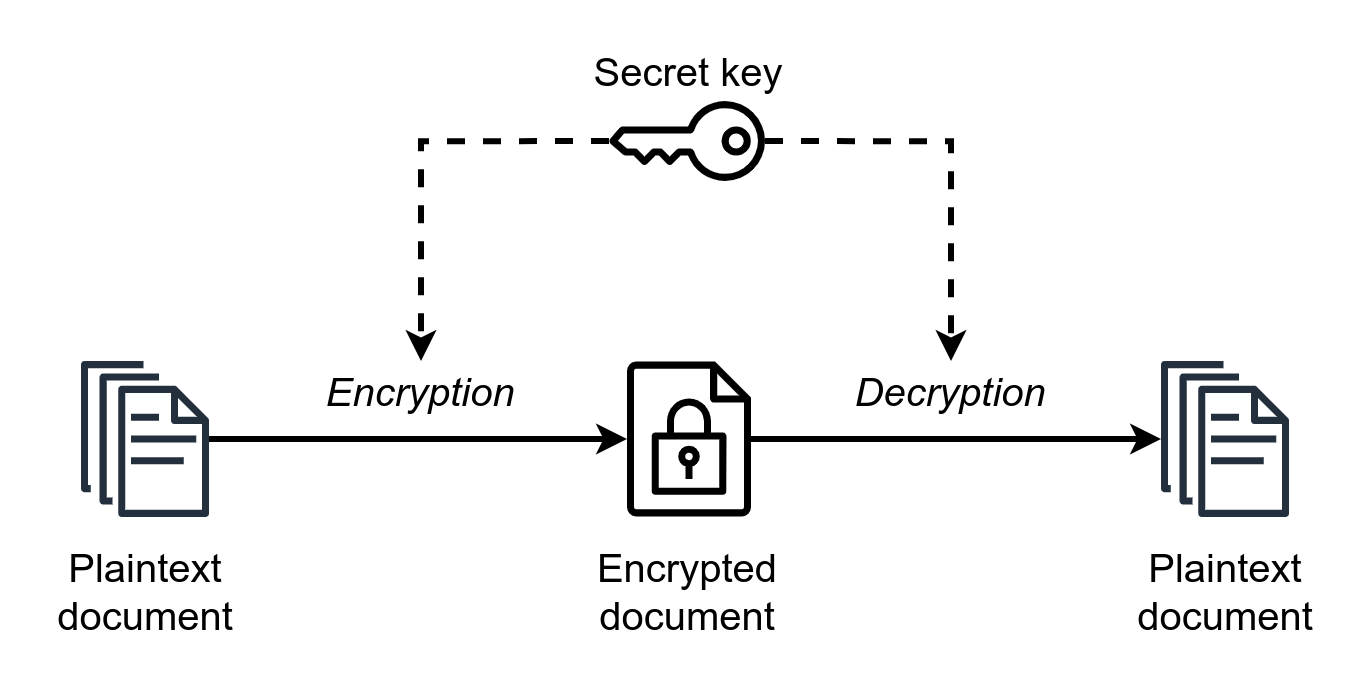
\includegraphics{sym-enc}
  \caption{Symmetric Encryption}
  \labfig{symenc}
\end{marginfigure}

SSH works by using symmetric and asymmetric encryption.
The data packets sent over the network are enctypted,
usually using AES symmetric encryption.
This ensures that even if the data packets are intercepted
by a man-in-the-middle attacker, they cannot be read
since they are encrypted.

To login into a remote server, all you need to do is
provide the username and the IP address or the domain
name of the server to the \texttt{ssh} command.

\begin{marginfigure}
  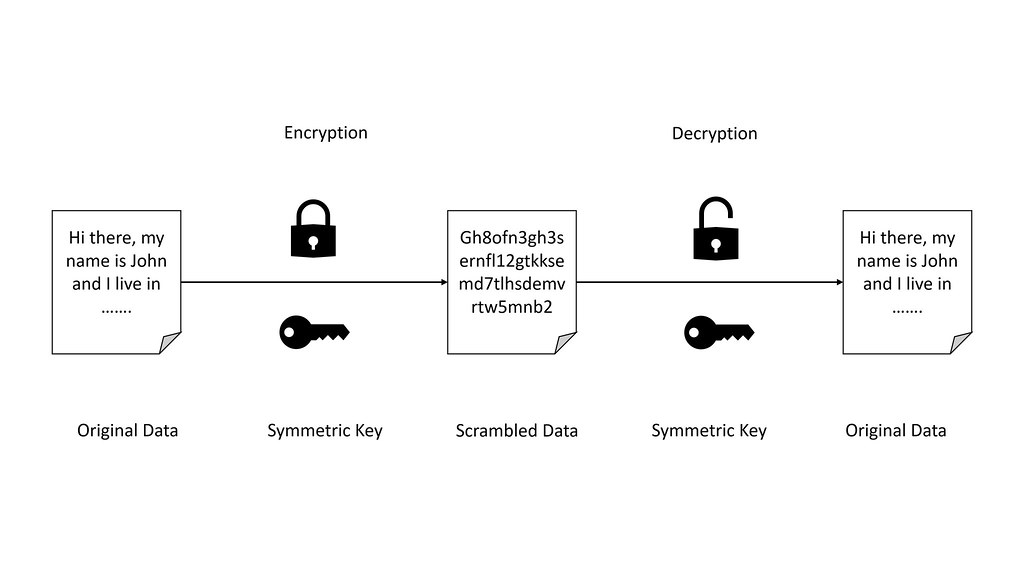
\includegraphics{encrypt}
  \caption{Symmetric Encryption}
  \labfig{encrypt}
\end{marginfigure}

\begin{lstlisting}[language=bash]
$ ssh username@ipaddress
\end{lstlisting}

\[
  \text{OR}
\]

\begin{lstlisting}[language=bash]
$ ssh username@domainname
\end{lstlisting}

SSH allows user to login to a remote server using
their username and password, but this is not encouraged
since it lets the user to be vulnerable to brute-force
attacks.

Another way to authenticate is by using public-private
key pairs.

\subsection{Key-based Authentication}

\begin{marginfigure}
  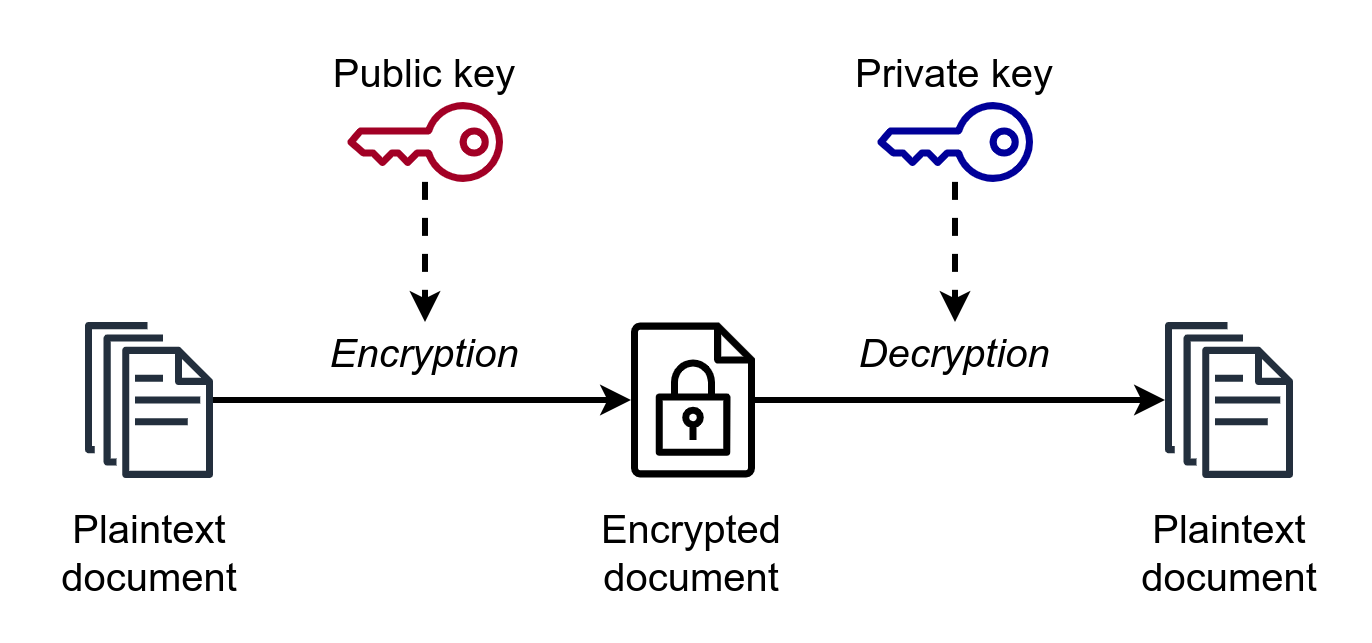
\includegraphics{ass-enc}
  \caption{Asymmetric Encryption}
  \labfig{ass-enc}
\end{marginfigure}

One of the most powerful features of SSH is its ability
to use public-private key pairs for authentication. In
our course, we emphasize the importance of this method.
Instead of relying on passwords, which can be vulnerable
to brute-force attacks, a pair of cryptographic keys is used.
The public key is stored on the server, while the private key
is kept secure on your local machine. This ensures a highly
secure and convenient way of accessing remote servers without
the need for constantly entering passwords.

\subsection{Configuring your SSH keys}

For this course, it is a must for you to not only
create, but also understand SSH keys.
Let us quickly see how to create a ssh key-pair
which can be used to login into a remote server.

We need to use the \texttt{ssh-keygen}
command to create a new public-private
key pair.

\begin{lstlisting}[language=bash]
$ ssh-keygen
Generating public/private ed25519 key pair.
Enter file in which to save the key (/home/test1/.ssh/id_ed25519):
\end{lstlisting}

Here you have to either simply press enter to
continue with the default location, or you can
also type a custom location where you want to
save the key. If this is your first time creating
keys, it is recommended to use the default location.

\begin{remark}
  There are multiple algorithms that can be used
  to generate a key pair. The most common ones are
  RSA, DSA, and ED25519. The ED25519 algorithm is
  the new default algorithm used by OpenSSH since
  it is shorter yet more secure than RSA.
  If you have an outdated version of OpenSSH, you
  might get the default RSA algorithm.
  To change the algorithm, you can use the \texttt{-t}
  flag along with the \texttt{ssh-keygen} command.
  \begin{lstlisting}[language=bash]
  $ ssh-keygen -t rsa \end{lstlisting}
  will create a RSA key pair and using
  \begin{lstlisting}[language=bash]
  $ ssh-keygen -t ed25519 \end{lstlisting}
  will create a ED25519 key pair.
\end{remark}

Next, it will ask you to enter a passphrase.
You can enter a passphrase for added security,
or you can simply press enter to continue without
a passphrase. If you do add a passphrase, you will
have to always enter the passphrase whenever you
use the key. We can continue without a passphrase
for now by pressing enter.

\begin{lstlisting}[language=bash]
Enter passphrase (empty for no passphrase):
Enter same passphrase again:

Your identification has been saved in /home/username/.ssh/id_ed25519
Your public key has been saved in /home/username/.ssh/id_ed25519.pub
The key fingerprint is:
SHA256:n4ounQd6v9uWXAtMyyq7CdncMsh1Zuac5jesWXrndeA test1@rex
The key's randomart image is:
+--[ED25519 256]--+
|                 |
|                 |
|                 |
|          .      |
|      . S+ .  .  |
|   . *.O o=... . |
|    =o=o*+++ .E .|
|    o.=Bo*O o. . |
|     +**XB.+.    |
+----[SHA256]-----+
\end{lstlisting}

Our key pair has been generated. The private key
is stored in \texttt{/home/username/.ssh/id\_ed25519}
and the public key is stored in
\texttt{/home/username/.ssh/id\_ed25519.pub}.

Make sure to \textbf{never} share your private key with anyone.
Ideally, you dont even need to see the private key yourself.
You should only share the public key with the server
you want to login to.

\subsection{Sharing your public key}

\textbf{ssh-copy-id}

Finally, to share the public key with the server,
there are usually multiple ways. If the server
allows you to login using a password, you can
simply use the \texttt{ssh-copy-id} command.
This command will take your username and password
to login to the server, and then copy the public
key which you provide to the server.

\begin{lstlisting}
$ ssh-copy-id -i /key/to/public/key username@ipaddress
\end{lstlisting}

\begin{remark}
  The \texttt{-i} flag is used to specify the path
  to the public key. You can drop the \texttt{.pub}
  from the path as well (making it the path to the
  private key), since \texttt{ssh-copy-id} will
  automatically look for the public key.
  However, this flag is not required if you
  are using the default location.
  This is why using the default location is
  recommended for beginners.
  The simplified syntax then becomes
  \begin{lstlisting}[language=bash]
  $ ssh-copy-id username@ipaddress \end{lstlisting}
  The same applies for logging into the server
  using the \texttt{ssh} command.
\end{remark}

\textbf{manual install}

However, most servers do not allow password login
at all, since it defeats the purpose of using
a public-private key pair. In such cases, you
need to somehow copy the public key to the server.

If you have physical access to the server, you
can simply copy the public key to the server
in the \texttt{~/.ssh/authorized\_keys} file
of the server.

\begin{lstlisting}[language=bash]
$ file ~/someoneskey.pub
~/someoneskey.pub: OpenSSH ED25519 public key
$ cat ~/someoneskey.pub >> ~/.ssh/authorized_keys
\end{lstlisting}

\begin{remark}
  Make sure to use the \texttt{>>} operator and
  not the \texttt{>} operator. The \texttt{>>}
  operator appends the contents of the file to
  the end of the file, while the \texttt{>}
  operator overwrites the file, we do not want that.
\end{remark}

\textbf{System Commands Course}

However, in case of our course, you do not have access
to the server as well. To submit your \textbf{public key},
you have to login into the website
\url{https://se2001.ds.study.iitm.ac.in/passwordless}
using your institute credentials, and then submit
your public key in the form provided.

You can print out the contents of the public key
using the \texttt{cat} command and copy the contents
into the form.

\begin{lstlisting}[language=bash]
[test1@rex ~]$ cat .ssh/id_ed25519.pub
ssh-ed25519 AAAAC3NzaC1lZDI1NTE5AAAAIDxh5EuvzQkGvsqlMQW3rOkY+wyo+2d6Y5CSqNGlLs2a test1@rex
\end{lstlisting}

You should copy the entire contents of the file, including
your username and hostname.

\subsection{How to login to a remote server}

You can then login into the server using the \texttt{ssh}
command.

\begin{lstlisting}[language=bash]
$ ssh rollnumber@se2001.ds.study.iitm.ac.in
\end{lstlisting}

\[
  \text{OR, if not using the default location of key}
\]

\begin{lstlisting}[language=bash]
$ ssh -i /path/to/private/key rollnumber@se2001.ds.study.iitm.ac.in
\end{lstlisting}

If successful, you will be logged into the server
and the prompt will change to the server's prompt.

\begin{lstlisting}[language=bash]
[test1@rex ~]$ ssh 29f1001234@se2001.ds.study.iitm.ac.in
Last login: Mon Jun  3 07:43:22 2024 from 192.168.2.3
29f1001234@se2001:~$
\end{lstlisting}

Notice that the prompt has changed from \texttt{test1@rex}
which was the prompt of your local machine, to
\texttt{rollnumber@se2001} which is the prompt of the
server.

\subsection{Call an exorcist, there's a daemon in my computer}

What is \texttt{sshd}?
It is a daemon.

\begin{definition}[Daemon]
  In multitasking computer operating systems, a daemon
  is a computer program that runs as a background process,
  rather than being under the direct control of an
  interactive user.
\end{definition}

There are many daemons running in your computer.
You can use \texttt{systemctl status} to see the
loaded and active daemons in your computer.

\begin{lstlisting}[language=bash]
$ systemctl status
* rex
    State: running
    Units: 419 loaded (incl. loaded aliases)
     Jobs: 0 queued
   Failed: 0 units
    Since: Thu 2024-06-13 12:55:42 IST; 7h ago
  systemd: 255.6-1-arch
   CGroup: /
           |-init.scope
           | `-1 /usr/lib/systemd/systemd --switched-root --system --deserialize=43
           |-system.slice
           | |-NetworkManager.service
           | | `-547 /usr/bin/NetworkManager --no-daemon
           | |-adb.service
           | | `-558 adb -L tcp:5037 fork-server server --reply-fd 4
           | |-avahi-daemon.service
           | | |-550 "avahi-daemon: running [rex.local]"
           | | `-557 "avahi-daemon: chroot helper"
           | |-cronie.service
           | | `-621 /usr/sbin/crond -n
           | |-cups.service
           | | `-629 /usr/bin/cupsd -l
           | |-dbus-broker.service
           | | |-545 /usr/bin/dbus-broker-launch --scope system --audit
\end{lstlisting}

Here you can see some of the important daemons running,
such as \texttt{NetworkManager} which is used to manage
the network connections, \texttt{cronie} which is used
to run scheduled tasks, \texttt{cups} which is used to
manage printers, etc.

\textbf{sshd}

sshd is the daemon that runs on the server and listens
to any incoming SSH connections. It is the daemon that
lets you login into the server using the SSH protocol.

Your own system might not be running the \texttt{sshd}
daemon, since you are not running a server. However,
you can check if the \texttt{sshd} daemon is running
using the \texttt{systemctl} command.

\begin{lstlisting}[language=bash]
$ systemctl status sshd
* sshd.service - OpenSSH Daemon
     Loaded: loaded (/usr/lib/systemd/system/sshd.service; disabled; preset: disabled)
     Active: inactive (dead)
\end{lstlisting}

Here you can see that the \texttt{sshd} daemon is
currently inactive. This is because I am not running
a server and don't usually login remotely to my
system. However, the output of the same command
would be something like as shown below
if it is enabled on your system.


\begin{lstlisting}[language=bash]
$ systemctl status sshd
* sshd.service - OpenSSH Daemon
     Loaded: loaded (/usr/lib/systemd/system/sshd.service; disabled; preset: disabled)
     Active: active (running) since Thu 2024-06-13 19:48:44 IST; 12min ago
   Main PID: 3583344 (sshd)
      Tasks: 1 (limit: 9287)
     Memory: 2.1M (peak: 2.3M)
        CPU: 8ms
     CGroup: /system.slice/sshd.service
             `-3583344 "sshd: /usr/bin/sshd -D [listener] 0 of 10-100 startups"

Jun 13 19:48:44 rex systemd[1]: Started OpenSSH Daemon.
Jun 13 19:48:45 rex sshd[3583344]: Server listening on 0.0.0.0 port 22.
Jun 13 19:48:45 rex sshd[3583344]: Server listening on :: port 22.
\end{lstlisting}

If we run the same command on the server, we can see
that it is running. However, we wont be able to
read the logs of the server, since we are not
authorized.

\begin{lstlisting}
$ ssh username@se2001.ds.study.iitm.ac.in
username@se2001:~$ systemctl status sshd
* ssh.service - OpenBSD Secure Shell server
     Loaded: loaded (/lib/systemd/system/ssh.service; enabled; vendor preset: enabled)
     Active: active (running) since Thu 2024-06-13 12:32:47 UTC; 1h 57min ago
       Docs: man:sshd(8)
             man:sshd_config(5)
    Process: 732 ExecStartPre=/usr/sbin/sshd -t (code=exited, status=0/SUCCESS)
   Main PID: 745 (sshd)
      Tasks: 1 (limit: 4557)
     Memory: 22.0M
        CPU: 8.769s
     CGroup: /system.slice/ssh.service
             `-745 "sshd: /usr/sbin/sshd -D [listener] 0 of 10-100 startups"

Warning: some journal files were not opened due to insufficient permissions.
\end{lstlisting}

\begin{remark}
  Notice that there are some differences in the output
  when run from my local system and from the system
  commands server. Such as, the name of the service
  is \texttt{ssh} on the server, while it is \texttt{sshd}
  on my local system. Also the full name is \texttt{OpenBSD
  Secure Shell server} on the server, while it is
  \texttt{OpenSSH Daemon} on my local system.
  The path of the service file is also different.
  This is because the server is running a ubuntu
  distribution whereas my local system runs an arch
  distribution. They have different packages for
  ssh, and hence the differences.
\end{remark}

\footnotetext{
  I have set the \texttt{LC\_ALL} environment variable
  to the locale C while generating the
  above outputs to prevent latex errors.
  Ideally if you run the command, you will see
  a prettier unicode output.
}

% % \setchapterpreamble[u]{\margintoc}
\chapter{Process Management}
\labch{procman}

\section{What is sleep?}

\lstinline|sleep| is a command that is used to delay the execution of a process
for a specified amount of time. \textbf{sleep} itself is a no-op command,
\footnote{
  NO-OP stands for No Operation. It is a command that does nothing.
  More reading on NO-OP can be found
  \href{https://en.wikipedia.org/wiki/NOP\_(code)}{here}.
}
but it takes a variable amount of time to execute, depending on the argument
of the command. This is useful when you want to delay the execution of another
command or chain of commands by a certain amount of time.

\subsection{Example}

\begin{lstlisting}[language=bash]
$ sleep 5
$ echo "Hello, World!"
Hello, World!
\end{lstlisting}

\subsection{Scripting with sleep}

If you run the above snippet, you will see that the output is delayed by 5 seconds.
Moreover, the prompt itself will not be available for 5 seconds, as the shell is busy
with executing the \lstinline|sleep| command.
To run the entire snippet as one process, simply put the two commands on
separate lines of a file (say, \lstinline|hello.sh|), and run the file as a script.

\begin{lstlisting}[language=bash]
$ cat hello.sh
sleep 5
echo "Hello, World!"
$ bash hello.sh
Hello, World!
\end{lstlisting}

We will be using \lstinline|sleep| in the examples throughout this chapter to demonstrate
process management since it is a simple command that can be used to quickly
spawn an idempotent process for any arbitrary amount of time.

\subsection{Syntax and Synopsis}

\begin{lstlisting}[language=bash]
sleep NUMBER[SUFFIX]...
\end{lstlisting}

Here the \lstinline|NUMBER| is the amount of time to sleep.
The \lstinline|SUFFIX| can be \lstinline|s| for seconds, \lstinline|m| for minutes,
\lstinline|h| for hours, and \lstinline|d| for days.

\vfill
\pagebreak
\section{Different ways of running a process}

\subsection{What are processes?}

\begin{definition}[Process]
  A process is an instance of a program that is being executed.
  It contains the program code and its current activity.
  Depending on the operating system (OS), a process may be made up of
  multiple threads of execution that execute instructions concurrently.
  Several processes may be associated with the same program; for example,
  opening up several instances of the same program often means more than
  one process is being executed.
  Each process has its own `process id` or \textbf{PID} to uniquely identify it.
\end{definition}

Whenever we run an application, or even a command on the linux shell, it spawns a process. Processes are always created by an already
existing process
\sidenote{
  Other than the very first process, which is always the
  \textbf{init} process. In most distributions, this is
  done by
  \href{https://systemd.io/}{systemd}, which is an
  init system that does a lot of other things as well.
  You can learn more about systemd and what all
  it does
  \href{https://documentation.suse.com/external-tree/en-us/sles/12-SP4/systemd\_in\_suse\_linux\_enterprise\_12\_white\_paper.pdf}{here}.
}
This creates a tree-like structure of processes, where each process has a parent process and can have multiple child processes.
When the parent of a process dies, the child processes are adopted by the \textbf{init} process.
\textbf{init} is thus the root of the process tree.

\begin{figure}[h!]
  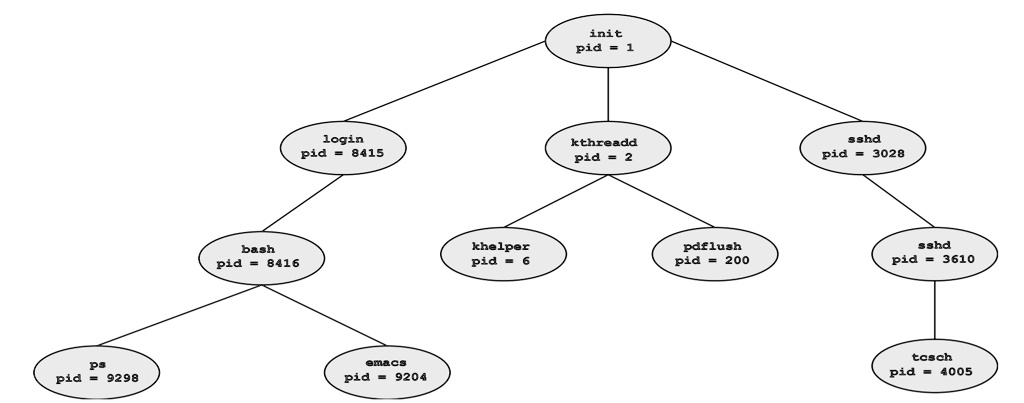
\includegraphics{process-tree}
  \caption{Example of a process tree}
  \labfig{process-tree}
\end{figure}

\subsection{Process Creation}
In linux systems, processes are managed by the kernel.
The kernel is responsible for creating, scheduling, and destroying processes.
The user can interact with the kernel using system calls to create, manage, and destroy processes.
Creating processes is simple, and can be done using the \textbf{fork()} system call.
This is used when any process wants to create a new process.

To simply create a new process for a command,
we can simply type in the command and press enter.
This will not only fork a new process from the terminal or
terminal emulator as the parent process, but also tie the
standard input, standard output, and standard error of the child process
to the terminal or terminal emulator.
\sidenote{
  Standard Input, Output, and Error are the default streams that are used by
  the shell to interact with the user. Standard Input is used to take input from
  the user, Standard Output is used to display output to the user, and Standard Error
  is used to display errors to the user. We will cover these in details in the next chapter.
}

\begin{lstlisting}[language=bash]
$ sleep 5
\end{lstlisting}

This will create a new process that will sleep for 5 seconds.

Remember that each process has a unique process id (PID).
Each process also has a parent process id (PPID),
which is the PID of the parent process.
If a process is created by the shell, the shell will be the parent process.
If the shell's process is killed, the child process will also
be killed, as the child process is owned by the shell.

\subsection{Process Ownership}

If you are using a linux operating system with a GUI server (X or Wayland),
try the following to understand how process ownership works.

Open two terminals, in the first one, run \lstinline|echo \$\$| to see the
process ID of that shell.
It should print out a random string of digits, that is the PID of the shell.
Then run a GUI application, such as \textbf{firefox}.
\sidenote{
  Make sure you are running something that is not running already.
}
This will block your terminal and open a new window of firefox.

\begin{lstlisting}[language=bash]
$ echo $$
2277503
$ firefox
\end{lstlisting}

Now in the other terminal, which is free, run \lstinline|pgrep firefox|
\sidenote{
  or whatever was your process's name
}
It should print out another random string of digits, it is the PID of
firefox.

Now you can use the following command to find the parent process's process
ID (PPID) to verify it is the same as the output of \lstinline|$$| in the first terminal.

\begin{lstlisting}[language=bash]
$ pgrep firefox
2278276
$ ps -efj | awk '$2==2278276;NR==1'
UID          PID    PPID    PGID     SID  C STIME TTY          TIME CMD
sayan    2278276 2277503 2278276 2277503 12 16:59 pts/5    00:00:03 /usr/lib/firefox/firefox
\end{lstlisting}

Here we can see that the PPID of firefox is the PID of the shell.

Note that the second command should put the PID of firefox, which we got
from the previous command. This can also be done in a single command
which you can directly copy and paste in your terminal.

\begin{lstlisting}[language=bash]
$ ps -efj | awk "\$2==$(pgrep firefox);NR==1"
UID          PID    PPID    PGID     SID  C STIME TTY          TIME CMD
sayan    2278276 2277503 2278276 2277503  1 16:59 pts/5    00:00:04 /usr/lib/firefox/firefox
\end{lstlisting}

Now, what happens if we kill the parent process?
To kill a process all we need to use is use the \lstinline|kill|
command with the PID of the process.

\begin{lstlisting}[language=bash]
$ kill -9 2277503
\end{lstlisting}

\marginnote{
  The \lstinline|-9| flag is used to send a \textbf{SIGKILL} signal to the process.
  This signal is used to kill a process immediately.
  We will cover signals later.
}

If you have been following along, you will see that both the terminal and firefox
dissapear from your screen. You will also notice that if you run the same
command to print the PID and PPID of firefox, it does not show anything.
This is because the process is killed and the process tree is destroyed, so
even firefox, being the child of the shell process, is killed.

\subsection{Don't kill my children}

However, there are also ways to create a new process in the background.
The easiest way to do this is to append an ampersand (\lstinline|&|) to the
end of the command. This is a shell syntax that tells the shell to fork the
command as a child process and run it in the background. What this means is
the shell will not wait for the command to finish, and will return the prompt
to the user immediately. However, the standard output and standard error may
still be tied to the terminal or terminal emulator. So if the process writes
something to the standard output or standard error, it will be displayed on the
terminal. Furthermore, the process is still owned by the shell, and if the shell
is killed, the process's parent will be changed to the \textbf{init} process.

Lets try the same exercise as earlier, but now with the \lstinline|&| at the end.

Open two terminals, and in the first one, execute the following command.

\begin{lstlisting}[language=bash]
$ echo $$
2400520
$ firefox &
[1] 2401297
$ echo "hello"
hello
$
ATTENTION: default value of option mesa_glthread overridden by environment.
$
\end{lstlisting}

You can observe that the firefox window opens up similar to last time, but
now the prompt returns immediately. You can also see that the output of the
\lstinline|echo| command is displayed on the terminal.

If you try to perform some operations in the browser, it may also print
some messages to the terminal screen, even though it is not waiting for
the command to finish. The "ATTENTION" message is an example of this.

Also observe that as soon as we launched \textbf{firefox}, it printed out
two numbers, [1] and 2401297. The number in the square brackets is the job
id of the process, and the number after that is the PID of the process.
So now we dont even need to use \lstinline|pgrep| to find the PID of the process.

Now in the other terminal, run the following command.

\begin{lstlisting}[language=bash]
$ ps -efj | awk "\$2==$(pgrep firefox);NR==1"
UID          PID    PPID    PGID     SID  C STIME TTY          TIME CMD
sayan    2401297 2400520 2401297 2400520  3 17:13 pts/5    00:00:08 /usr/lib/firefox/firefox
\end{lstlisting}

Still we can see that the PPID of firefox is the PID of the shell.

Now, if we kill the parent process, the child process will be adopted by the
init process, and will continue to run.

\begin{lstlisting}[language=bash]
$ kill -9 2400520
\end{lstlisting}

If you re-run the command to print the PID and PPID of firefox, you will see
that the PPID of firefox is now set to $1$, which is the PID of the \textbf{init}
command.

\begin{lstlisting}[language=bash]
$ ps -efj | awk "\$2==$(pgrep firefox);NR==1"
UID          PID    PPID    PGID     SID  C STIME TTY          TIME CMD
sayan    2401297       1 2401297 2400520  3 17:13 ?        00:00:09 /usr/lib/firefox/firefox
\end{lstlisting}

You can also see that the TTY column is now set to \lstinline|?|, which means that
the process is no longer tied to the terminal.

However, if instead of killing the parent process using the \textbf{SIGKILL}
signal, if you sent the \textbf{SIGHUP} signal to the parent, the child process
will still be terminated, as it will propagate the hangup signal to the child process.


\subsection{Setsid}

So how do we start a process directly in a way that it is not tied to the terminal?
Many times we would require to start a process in the background to run
asynchronously, but not always do we want to see the output of the process
in the terminal from where we launched it. We may also want the process
to be owned by the \textbf{init} process from the get go.

To do this, we can use the \lstinline|setsid| command. This command is used to
run a command in a new session. This will create a new process group and
set the PPID of the process to the \textbf{init} process. The TTY will also
be set to \lstinline|?|.

Lets try the same exercise with the \lstinline|setsid| command.
Open two terminals, in one of them, run the following command.

\begin{lstlisting}[language=bash]
$ echo $$
2453741
$ setsid -f firefox
$
\end{lstlisting}

Observe that firefox will open up, but the prompt will return immediately.

In another terminal, run the following command.

\begin{lstlisting}[language=bash]
$ ps -efj | awk "\$2==$(pgrep firefox);NR==1"
UID          PID    PPID    PGID     SID  C STIME TTY          TIME CMD
sayan    2454452       1 2454452 2454452  2 17:19 ?        00:00:07 /usr/lib/firefox/firefox
\end{lstlisting}

Observe that even without killing the parent process, the PPID of firefox is
already set to $1$, which is the PID of the \textbf{init} process.
So the process will not be killed if the shell is killed.

This is called a hang-up signal. We can still artificially send the
\textbf{SIGHUP} signal, which tells firefox that its parent has stopped
by using the \lstinline|kill -1| command.

\begin{lstlisting}[language=bash]
$ kill -1 2454452
\end{lstlisting}

This will still close firefox, even though the parent process (\textbf{init})
didn't actually get killed.

\subsection{Nohup}

If you do not want to give up the ownership of a child process,
and also don't really need to get the prompt back, but you do not
want to see the output of the command in your terminal. You can
use the \lstinline|nohup| command followed by the command you want to
run. It will still be tied to the terminal, and you can use
\lstinline|Ctrl+C| to stop it, \lstinline|Ctrl+Z| to pause it, etc.
The prompt will also be blocked till the process runs.
However, the input given to the terminal will not be sent
to the process, and the output of the process will not be
shown on the terminal. Instead, the output will be saved
in a file named \lstinline|nohup.out| in the current directory.

However, this is different from simply running the command
with a redirection operator (\lstinline|>|) at the end,
\sidenote{
  We will cover redirection operators in the next chapter.
}
because the \lstinline|nohup| command also makes the process
immune to the hang-up signal.

\begin{exercise}
  Try the same exercise as before, but this time use the \lstinline|nohup|
  to run firefox, then in another terminal, find the PID and PPID of
  firefox. Then try to kill the parent process and see if firefox
  dies or not.
\end{exercise}

\subsection{coproc}

The \lstinline|coproc| command is used to run a command in the background
and tie the standard input and standard output of the command to a
file descriptor. This is useful when you want to run a command in the
background, but still want to interact with it using the shell.
This creates a two way pipe between the shell and the command.

\textbf{Syntax}

\begin{lstlisting}[language=bash]
$ coproc [NAME] command [redirections]
\end{lstlisting}

This creates a coprocess named \lstinline|NAME| and runs the command in the background.
If the \lstinline|NAME| is not provided, the default name is \lstinline|COPROC|.

However, the recommended way to use \lstinline|coproc| is to use it in a
subshell, so that the file descriptors are automatically closed when
the subshell exits.

\begin{lstlisting}[language=bash]
$ coproc [NAME] { command; }
\end{lstlisting}

coproc can execute simple commands or compound commands. For simple
commands, name is not possible to be specified. Compound commands like
loops or conditionals can be executed using coproc in a subshell.

The name that is set becomes a array variable in the shell, and can be used
to access the file descriptors for stdin, stdout, and stderr.

For example, to provide input to the command, you can use \lstinline|echo| and
redirection operators to write to the file descriptor.

Similarly you can use the \lstinline|read| command to read from the file descriptor.

\begin{lstlisting}[language=bash]
$ coproc BC { bc -l; }
$ jobs
[1]+  Running                 coproc BC { bc -l; } &
$ echo 22/7 >&"${BC[1]}"
$ read output <&"${BC[0]}"
$ echo $output
3.14285714285714285714
\end{lstlisting}

This uses concepts from redirection and shell variables, which we will cover
in later weeks.

\subsection{at and cron}

Processes can also be scheduled to be launched at a later time.
This is usually done using \textbf{cron} or the \textbf{at} command.
We will cover these in depth later.

\subsection{GNU parallel}

GNU parallel is a shell tool for executing jobs in parallel using one
or more computers. A job can be a single command or a small script that
has to be run for each of the lines in the input. The typical input is
a list of files, a list of hosts, a list of users, a list of URLs, or a
list of tables. A job can also be a command that reads from a pipe.
GNU parallel can then split the input into blocks and pipe a block
into each command in parallel.

\subsection{systemd services}

Finally, the best way to run a background process or a daemon is to use
\textbf{systemd} services. \textbf{systemd} is an init system that is
used by most modern linux distributions. You can create a service file
declaring the process, the command line arguments, the environment variables,
and the user and group that the process should run as. You can also
specify if the process should be restarted if it crashes, or if it should
be started at boot time.


\vfill
\pagebreak
\section{Process Management}
\subsection{Disown}

Disown is a shell builtin command that is used to remove a job from the shell's
job table. This is useful when you have started a process in the background
and you want to remove it from the shell's job table, so that it is not
killed when the shell is killed. What it means is that if the parent
process recieves a hang-up signal, it will not propagate it to the child
job if it is removed from the job table.
This is applicable only for processes started from a shell.

Open two terminals, in one, open firefox in background using the \lstinline|&|

\begin{lstlisting}[language=bash]
$ firefox &
$
\end{lstlisting}

and then in the other terminal, run the following command.

\begin{lstlisting}[language=bash]
$ ps -efj | awk "\$2==$(pgrep firefox);NR==1"
UID          PID    PPID    PGID     SID  C STIME TTY          TIME CMD
sayan    3216429 3215856 3216429 3215856 69 18:45 pts/5    00:00:02 /usr/lib/firefox/firefox
$ kill -1 3215856
\end{lstlisting}

Observe that firefox will close, even though it was running in the background.
This is because the shell will propagate the hang-up signal to the child process.
If the parent shell was forcefully killed using the \textbf{SIGKILL} signal,
then it wont have the opportunity to propagate the hang-up signal to the child process.
This is a separate process than the natural killing of firefox running in
foreground even when shell is killed with \textbf{SIGKILL} signal.

Now, to fix this, we can simply run the \lstinline|disown| command in the terminal
where we started the firefox process.

Again open a terminal emulator and run the following command.

\begin{lstlisting}[language=bash]
$ firefox &
$ disown
$
\end{lstlisting}

Now, in the other terminal, run the following command.

\begin{lstlisting}[language=bash]
$ ps -efj | awk "\$2==$(pgrep firefox);NR==1"
UID          PID    PPID    PGID     SID  C STIME TTY          TIME CMD
sayan    3216429 3215856 3216429 3215856 69 18:45 pts/5    00:00:02 /usr/lib/firefox/firefox
$ kill -1 3215856
$ ps -efj | awk "\$2==$(pgrep firefox);NR==1"
UID          PID    PPID    PGID     SID  C STIME TTY          TIME CMD
sayan    3216429       1 3216429 3215856 10 18:45 ?        00:00:03 /usr/lib/firefox/firefox
\end{lstlisting}

Firefox does not close anymore, even when the parent process is hanged up.

\subsection{Jobs}

To list the jobs that are running in a shell, you can use the \lstinline|jobs| command.

\begin{lstlisting}[language=bash]
$ firefox &
$ sleep 50 &
$ jobs
[1]-  Running                 firefox &
[2]+  Running                 sleep 50 &
\end{lstlisting}

Here \lstinline|+| denotes the current job, and \lstinline|-| denotes the previous job.
The first column is the job number, it can also be used to refer to the job
inside that same shell. The process ID of a process can be used to refer to
the process from anywhere, but the job ID is only valid in the shell where
it is created.

The process id can be listed using the \lstinline|jobs -l| command.

\begin{lstlisting}[language=bash]
$ jobs -l
[1]- 3303198 Running                 firefox &
[2]+ 3304382 Running                 sleep 50 &
\end{lstlisting}

Using disown removes the job from this table. We can selectively
remove only some jobs from the table as well.

\begin{lstlisting}[language=bash]
$ jobs
[1]-  Running                 firefox &
[2]+  Running                 sleep 50 &
disown %1
$ jobs
[2]+  Running                 sleep 50 &
\end{lstlisting}

Whereas using \lstinline|disown -a| will remove all jobs from the table.
\lstinline|disown -r| will remove only running jobs from the table.

If you dont really want to lose the job from the table, but you want to
prevent it from being killed when the shell is killed, you can use
\lstinline|disown -h| to mark the jobs to be ignored by the hang-up signal.
It will have same effect as last exercise, but it will still be present
in the output of the \lstinline|jobs| command.

\subsection{Suspending and Resuming Jobs}

Sometimes you may want to pause a job and resume it later.
This is supported directly by the linux kernel.
To pause any process you can send it the \textbf{SIGSTOP} or \textbf{SIGTSTP} signal.
\sidenote{
  The difference between \textbf{SIGSTOP} and \textbf{SIGTSTP} is that
  \textbf{SIGSTOP} is a signal that cannot be caught or ignored by the process,
  so the process will be paused immediately. \textbf{SIGTSTP} is a signal that
  can be caught or ignored by the process, so the process can do some cleanup
  before pausing. The default action of \textbf{SIGTSTP} is to pause the process.
}
This can be done using the same \textbf{kill} command. The signal number for
\textbf{SIGSTOP} is 19, and for \textbf{SIGTSTP} is 20.

To resume the process, you can send it the \textbf{SIGCONT} signal.
The signal number for \textbf{SIGCONT} is 18.

\begin{exercise}
  Try to pause a job using the \textbf{SIGSTOP} signal, then resume it using the
  \textbf{SIGCONT} signal.
  Open firefox from a terminal using \lstinline|firefox \&| and note the PID,
  then pause it using
  \lstinline|kill -19 <PID>|,
  try to click on the firefox window, and see if it responds.
  Then resume it using \lstinline|kill -18 <PID>|.
  Does the firefox window respond now?
\end{exercise}

If you start a command from the shell without using the \lstinline|&| operator,
you can pause the command using \lstinline|Ctrl+Z| and resume it using the
\lstinline|fg| command.
This sends the same signals as above, and uses the shell's job table
to keep track of the jobs.

\begin{remark}
  Just like disown, the \lstinline|fg| command can also take the job number
  as an argument to bring that job to the foreground. The default job
  is the current job. (Marked with a \lstinline|+| in the \lstinline|jobs| command))
\end{remark}

You can also use the \lstinline|bg| command to resume a job, but in the background.
This has same effect as using the \lstinline|&| operator at the end of the command.

\begin{remark}
  Since the disown, fg, and bg commands work on the shell's job table,
  they are shell builtins, and not a executable binary.
  You can verify this using the \lstinline|type| command.
\end{remark}

You cannot perform job control on a process that is not started from the shell,
or if you have disowned the process.

\subsection{Killing Processes}

We have been using the \lstinline|kill| command to send signals to processes.
The kill command is a shell builtin and an executable command that is used
to send signals to processes. The default signal that is sent is the
\textbf{SIGTERM} signal, which is signal number 15.
The kill command is the user-land way to communicate with the kernel that
some process needs to be given a certain signal.

\textbf{Syntax}

\begin{lstlisting}[language=bash]
$ kill [-signal|-s signal] PID|name...
\end{lstlisting}

Let us also briefly discuss what the synopsis of the command means, and
how to interpret it.

The first word is the name of the command, which is \lstinline|kill| in this case.
The argument \textbf{signal} inside square brackets means that it is optional.
The argument \textbf{PID} is the process ID of the process that you want to kill.
The argument \textbf{name} is the name of the process that you want to kill.
The pipe between \textbf{PID} and \textbf{name} means that you can provide
either the PID or the name of the process.
The ellipsis (\lstinline|...|) after \textbf{PID|name} means that you can provide
as many PIDs or names as you want.

\begin{remark}
  As mentioned, kill is also a shell builtin command. This means that
  the synopsis seen in the man page of kill is not the same as the
  synopsis of the builtin. The bash builtin of kill does not support
  providing names of the processes, only the PIDs. Hence if you want
  to kill a process by its name, you will either have to use the
  path of the kill binary, or use the \lstinline|pkill| command.
\end{remark}

So for example, we can run kill in the following manners.

\begin{lstlisting}[language=bash]
$ kill 2452
$ kill -9 2452
$ kill -9 2452 62
$ kill -SIGKILL 2525
$ kill -SIGKILL 2525 732
\end{lstlisting}

The \lstinline|kill| command can also be used to send other non-terminating signals
to the process. For example, the \textbf{SIGSTP} signal can be used to pause
a process, and the \textbf{SIGCONT} signal can be used to resume a process.
Similarly, there are some undefined signals that can be used to send custom
signals to the process.

\textbf{SIGUSR1} and \textbf{SIGUSR2} are signals that do not have any predefined
behaviour, and can be used by the user to send custom signals to the process.
The behaviour of the process on receipt of these signals is decided by the
process and told to the user by the process documentation. The user can
then send these signals to the process using the \lstinline|kill| command.
This helps user interact with processes that are not running directly in the
foreground of a shell.

Processes can also \textbf{trap} signals, which means that they can catch
a signal and run a custom handler function. This is useful when you want
to do some cleanup before the process is killed. This can also be used
to totally change how the process behaves on receipt of a signal.
However, to prevent malicious code from running, the \textbf{SIGKILL} signal
cannot be trapped, and the process will be killed immediately. Similarly
the \textbf{SIGSTOP} signal, which is similar in definition to the \textbf{SIGSTP}
signal, cannot be trapped.

To see the list of the signals, we can run \lstinline|kill -l|.

\begin{lstlisting}[language=bash]
$ kill -l
 1) SIGHUP       2) SIGINT       3) SIGQUIT      4) SIGILL       5) SIGTRAP
 6) SIGABRT      7) SIGBUS       8) SIGFPE       9) SIGKILL     10) SIGUSR1
11) SIGSEGV     12) SIGUSR2     13) SIGPIPE     14) SIGALRM     15) SIGTERM
16) SIGSTKFLT   17) SIGCHLD     18) SIGCONT     19) SIGSTOP     20) SIGTSTP
21) SIGTTIN     22) SIGTTOU     23) SIGURG      24) SIGXCPU     25) SIGXFSZ
26) SIGVTALRM   27) SIGPROF     28) SIGWINCH    29) SIGIO       30) SIGPWR
31) SIGSYS      34) SIGRTMIN    35) SIGRTMIN+1  36) SIGRTMIN+2  37) SIGRTMIN+3
38) SIGRTMIN+4  39) SIGRTMIN+5  40) SIGRTMIN+6  41) SIGRTMIN+7  42) SIGRTMIN+8
43) SIGRTMIN+9  44) SIGRTMIN+10 45) SIGRTMIN+11 46) SIGRTMIN+12 47) SIGRTMIN+13
48) SIGRTMIN+14 49) SIGRTMIN+15 50) SIGRTMAX-14 51) SIGRTMAX-13 52) SIGRTMAX-12
53) SIGRTMAX-11 54) SIGRTMAX-10 55) SIGRTMAX-9  56) SIGRTMAX-8  57) SIGRTMAX-7
58) SIGRTMAX-6  59) SIGRTMAX-5  60) SIGRTMAX-4  61) SIGRTMAX-3  62) SIGRTMAX-2
\end{lstlisting}

Some of the important signals are:

\begin{itemize}
  \item \textbf{SIGHUP} - Hangup signal. This is sent to a process when the
  terminal is closed. This is used to tell the process that the terminal
  is no longer available.
\item \textbf{SIGINT} - Interrupt signal. This is sent to a process when the
  user presses \lstinline|Ctrl+C|. This is used to tell the process to stop
  what it is doing and exit.
\item \textbf{SIGKILL} - Kill signal. This is used to kill a process immediately.
  This signal cannot be caught or ignored by the process.
\item \textbf{SIGTERM} - Terminate signal. This is used to tell the process
  to exit gracefully. The process can catch this signal and do some cleanup
  before exiting. This is the default signal sent by the \lstinline|kill| command.
\item \textbf{SIGSTP} - Stop signal. This is used to pause a process.
  This is sent when the user presses \lstinline|Ctrl+Z|. This signal can be
  caught or ignored by the process.
\item \textbf{SIGSTOP} - Stop signal. This is used to pause a process.
  This signal cannot be caught or ignored by the process.
\item \textbf{SIGCONT} - Continue signal. This is used to resume a process
  that has been paused using the \textbf{SIGSTOP} signal. This is sent
  when the user presses \lstinline|fg| or \lstinline|bg|.
\item \textbf{SIGUSR1} - User defined signal 1. This is a signal that can
  be used by the user to send a custom signal to the process.
\item \textbf{SIGUSR2} - User defined signal 2. This is a signal that can
  be used by the user to send a custom signal to the process.
\item \textbf{SIGCHLD} - Child signal. This is sent to the parent process
  when a child process exits. This is used to tell the parent process that
  the child process has exited.
\item \textbf{SIGSEGV} - Segmentation fault signal. This is sent to a process
  when it tries to access memory that it is not allowed to access.
\item \textbf{SIGPIPE} - Pipe signal. This is sent to a process when it tries
  to write to a pipe that has been closed.
\end{itemize}

\vfill
\pagebreak
\section{Finding Processes}

As we saw, managing a process is easy once we know the PID of the process.
However, it is not always easy to find the PID of a process.
To do this, there are multiple tools in linux that can be used.

\subsection{pgrep}

The \lstinline|pgrep| command is used to find the PID of a process based on its name.
It can take the name of the process as an argument, and will print the PID of the
processes that match the name. The search can also be a regex pattern.
\sidenote{
  We will discuss regex patterns in the next chapter.
}
We have already seen how \lstinline|pgrep| can be used to find the PID of a process.

\begin{lstlisting}[language=bash]
$ pgrep firefox
526272
\end{lstlisting}

We can also use it for any process run from the terminal.

\begin{lstlisting}[language=bash]
$ sleep 50 &
$ sleep 20 &
$ sleep 10 &
$ pgrep sleep
98963
99332
99526
\end{lstlisting}

\subsection{pkill}

Similarly, we also have the \lstinline|pkill| command, which is used to kill a process
based on its name. It can take the name of the process as an argument, and will
send the \textbf{SIGTERM} signal to the processes that match the name.
Other signals can also be sent using the \lstinline|-signal| flag, similar to the
kill command.

\begin{lstlisting}[language=bash]
$ pkill firefox
\end{lstlisting}

\subsection{pidwait}

The \lstinline|pidwait| command is used to wait for a process to exit.
It searches for the process using its name, a part of its name, or any
regex matching its name, and waits for the process to exit.

\begin{exercise}
  Open firefox from a terminal in the background, then use the \lstinline|pidwait|
  to wait till the process exits. After some time, close the firefox window
  and observe the terminal.
\end{exercise}

\vfill
\pagebreak
\section{Listing Processes}

Sometimes we may not even know the name of the process, and we may want to
list all the processes running on the system. This can be done using the
many commands.

\subsection{ps}

\textbf{ps} is an ancient command
\sidenote{
  It exists in the Unix V7 manual, which was released in 1979.
  It has BSD-like options, GNU-like options, and System V-like options.
}
that is used to list the processes running on the system.

There are a lot of options and flags that can be used with the \textbf{ps} command.
The flags are of multiple types, and some flags perform the same function but
are named differently. This is because the \textbf{ps} command has been around
for a long time, and has been implemented in multiple ways in different systems.
There are also different formats in which the output can be displayed.

The most common flags used with the \textbf{ps} command are:

\begin{itemize}
  \item \textbf{ps} - This will get a snapshot of the processes owned by the user tied to the TTY.
  \item \textbf{ps -e} - This will show all the processes.
  \item \textbf{ps -f} - This will show full format listing.
  \item \textbf{ps -l} - This will show long format listing.
  \item \textbf{ps u} - This will show user-oriented format listing.
  \item \textbf{ps x} - This will show processes without controlling terminals.
  \item \textbf{ps -A} - This will show all processes.
  \item \textbf{ps aux} - This is a common command to see all processes owned by all users with and without TTY associations and showing the user who owns them.
  \item \textbf{ps --forest} - This will show the processes in a tree form.
\end{itemize}

There are hundreds of flags that can be used with the \textbf{ps} command.

\begin{exercise}
  Try to use the \textbf{ps} command with the flags mentioned above, and see
  the output of the command.
\end{exercise}

\subsection{pstree}

The \textbf{pstree} command is used to display the processes in a tree form.
Although the \textbf{ps} command can also display the processes in a tree form
using the \lstinline|--forest| flag, the \textbf{pstree} command is more suited
for this purpose. It has many features that ps lacks, such as collapsing
branches of identical processes, better ASCII art, Unicode support, etc.

If the system and the terminal supports unicode, the \textbf{pstree} command
will automatically use
\href{https://en.wikipedia.org/wiki/Box-drawing\_character}{VT100 box-drawing characters}
to make the tree look better. We can still force it to use ASCII with the
\lstinline|-A| flag.

We can also disable the clubbing of identical processes using the \lstinline|-c| flag.

The pstree command optionally takes a PID as an argument, and will display
the tree rooted at that PID. If no PID is provided, it will display the
tree rooted at the init process.

I can find the PID of the tmux server I am running to develop this book
using the \lstinline|pgrep| command.
\begin{lstlisting}[language=bash]
$ pgrep tmux
62957
\end{lstlisting}

And then use the \lstinline|pstree| command
to display the tree rooted at that PID.

\begin{lstlisting}[language=bash]
$ pstree -A 62957
tmux: server-+-bash---nvim-+-nvim-+-node---14*[{node}]
             |             |      |-texlab---9*[{texlab}]
             |             |      |-xsel
             |             |      `-9*[{nvim}]
             |             `-2*[{nvim}]
             |-bash---watch.sh---entr
             |-bash---zathura---8*[{zathura}]
             |-3*[bash]
             |-2*[bash---man---less]
             |-bash---nvim-+-nvim-+-2*[node---9*[{node}]]
             |             |      `-{nvim}
             |             `-2*[{nvim}]
             `-bash-+-pstree
                    `-xsel
\end{lstlisting}

This helps us easily find out which processes are running under which process,
and helps us understand the process tree.

\subsection{top}

The \textbf{top} command is used to display the processes that are running
in real time. It is an interactive command that displays the processes in
a table format, and updates the table every few seconds. It also displays
the CPU and memory usage of the processes.

The \textbf{top} command is very useful when you want to monitor the processes
and the resources they are using in real time. It is also useful when you
want to find out which process is using the most CPU or memory.

Since it is an interactive command, it has keyboard shortcuts as well, along
with runtime options that can be used to change the behaviour of the command.

\marginnote{
  Note: The output of the \textbf{top} command is not static, and it contains
  control characters and
  \href{https://en.wikipedia.org/wiki/ANSI\_escape\_code}{ANSI escape codes}
  to make the output beautiful and interactive. This is why the output is not
  suitable for use in scripts, and is only meant for human consumption.
  I have removed the control characters and ANSI escape codes from the output
  shown here.
}

\begin{lstlisting}
$ top
top - 15:44:55 up 40 min,  1 user,  load average: 2.03, 1.37, 1.02
Tasks: 271 total,   1 running, 270 sleeping,   0 stopped,   0 zombie
%Cpu(s):  9.8 us,  4.9 sy,  0.0 ni, 85.4 id,  0.0 wa,  0.0 hi,  0.0 si,  0.0 st
MiB Mem :   7764.2 total,    604.5 free,   5663.2 used,   1919.6 buff/cache
MiB Swap:  20002.0 total,  19901.2 free,    100.8 used.   2101.0 avail Mem

    PID USER      PR  NI    VIRT    RES    SHR S  %CPU  %MEM     TIME+ COMMAND
    631 sayan     20   0 1248084  81976  44580 S  18.2   1.0   1:39.82 Xorg
   1072 sayan     20   0 3159356 229336  89816 S   9.1   2.9   0:44.01 spotify
   1079 sayan     20   0 1123.5g 128252  65776 S   9.1   1.6   0:09.37 Discord
      1 root      20   0   22076  12840   9476 S   0.0   0.2   0:03.62 systemd
      2 root      20   0       0      0      0 S   0.0   0.0   0:00.00 kthreadd
      3 root      20   0       0      0      0 S   0.0   0.0   0:00.00 pool_wo+
\end{lstlisting}

\subsection{htop}

The \textbf{htop} command is an interactive process viewer for Unix systems.
It is inspired from the \textbf{top} command, but has a lot more features
such as scrolling the process list, searching for processes, killing processes,
tree view of processes, etc.

\begin{exercise}
  Run (Install if not present) the \textbf{htop} command and see the output.
  Notice how the output is more interactive and colourful than the \textbf{top}
  command. Run something heavy in the background, and see how the CPU and
  the memory usage changes in real time.
\end{exercise}

One such command to run to simulate heavy CPU usage is to run the following command.

\begin{lstlisting}[language=bash]
$ cat /dev/urandom | gzip > /dev/null &
\end{lstlisting}

This will compress the random data from \lstinline|/dev/urandom| and write it to
\lstinline|/dev/null|. This will use a lot of CPU, and you can see the CPU usage
spike up. But this is a single core process, so the CPU usage will be limited
to only one core. However, the CPU core used may keep changing.

\begin{remark}
  The above command is a simple way to generate CPU usage. It will not
  write any data to disk and not eat any disk space. However, the
  command should be typed carefully, since if you forget to add the
  \lstinline|> /dev/null| part, it will write the compressed data to the
  terminal if \lstinline|-f| is given to \lstinline|gzip|, and the terminal
  will be filled with random data and get messed up. In this case
  you can type \lstinline|tput reset| to reset the terminal after killing
  the process.
\end{remark}

\subsection{btop}

The \textbf{btop} command is a terminal based graphical process viewer.
It is inspired from the \textbf{htop} command, but has a more graphical
interface. It is written in python, and uses the \textbf{blessings} library
to draw the interface.

\subsection{glances}

The \textbf{glances} command is a cross-platform monitoring tool that is
used to monitor the system resources in real time. It is written in python,
and uses the \textbf{curses} library to draw the interface.


\vfill
\pagebreak
\section{Exit Codes}

Every process that runs in linux has an exit code when it terminates.
This is a number that is returned by the process to the parent process
when it exits. This number is used to tell the parent process if the
process exited successfully or not. The exit code is a number between
0 and 255, and is used to tell the parent process the status of the
child process.

The exit code of the last run process is stored in a variable
called \lstinline|$?| in the shell. Successful processes return 0,
whereas unsuccessful processes return a non-zero number.
The exact return code is decided by the process itself, and usually
has some meaning to the process. Some common exit codes are:

\begin{itemize}
  \item 0 - Success
  \item 1 - General error
  \item 2 - Misuse of shell builtins
  \item 126 - Command invoked cannot execute
  \item 127 - Command not found
  \item 128 - Invalid argument to exit
  \item 128+n - Fatal error signal "n"
  \item 130 - Script terminated by \lstinline|Ctrl+C|
  \item 137 - Process killed with \textbf{SIGKILL}
  \item 255 - Exit status out of range
\end{itemize}

\begin{remark}
Note that $130=128+2$, and $2$ is the signal number for \textbf{SIGINT},
thus, the exit code for a process that is terminated by \lstinline|Ctrl+C|
is 130. Similarly, any other signal sent to the process causing it to
exit abnormally will have an exit code of $128+n$, where $n$ is the signal
number. Similarly $137=128+9$, and $9$ is the signal number for \textbf{SIGKILL}.
\end{remark}

To return any exit status from your script, you can use the \lstinline|exit| command.

\begin{lstlisting}[language=bash]
$ cat myscript.sh
#!/bin/bash
echo "hello"
exit 25
$ ./script.sh
bash: ./script.sh: No such file or directory
$ echo $?
127
$ ./myscript.sh
bash: ./myscript.sh: Permission denied
$ echo $?
126
$ chmod u+x myscript.sh
$ ./myscript.sh
hello
$ echo $?
25
\end{lstlisting}

The exit code is how shell constructs like \lstinline|if|, \lstinline|while|,
and \lstinline|until| construct their conditions. If the exit code is 0,
then it is considered true, and if the exit code is non-zero, then it
is considered false.

\begin{lstlisting}[language=bash]
$ if ./myscript.sh; then echo "success"; else echo "failure $?"; fi
hello
failure 25
$ if ls /bin/bash; then echo "success"; else echo "failure $?"; fi
/bin/bash
success
\end{lstlisting}

% % \setchapterpreamble[u]{\margintoc}
\chapter{Streams, Redirections, Piping}
\labch{redirection}

\section{Multiple Commands in a Single Line}

Sometimes we may want to run multiple commands in a single line.
For example, we may want to run two commands \lstinline|ls| and \lstinline|wc|
in a single line. We can do this by separating the commands with a semicolon.
This helps us see the output of both the commands without having the
prompt in between.

For example, the following command will run \lstinline|ls| and \lstinline|wc| in a single line.

\begin{lstlisting}[language=bash]
$ ls; wc .bashrc
docs  down  music  pics  programs  scripts  tmp  vids
  340  1255 11238 .bashrc
\end{lstlisting}

In this way of executing commands, the success or failure of one
command does not affect the other command. Concisely, the commands
are executed independently and sequentially. Even if a command
fails, the next command will be executed.

\begin{lstlisting}[language=bash]
$ date; ls /nonexistant ; wc .bashrc
Wed Jul  3 06:54:45 PM IST 2024
ls: cannot access '/nonexistant': No such file or directory
  340  1255 11238 .bashrc
\end{lstlisting}

\subsection{Conjunction and Disjunction}

We can also run multiple commands in a single line using conjunction
and disjunction. The conjunction operator \lstinline|&&| is used to run
the second command only if the first command is successful. The disjunction
operator \lstinline|||| is used to run the second command only if the first
command fails. In computer science, these operators are also known as
short-circuit logical \textbf{AND} and \textbf{OR} operators.
\sidenote{
  A short-circuit logical \textbf{AND} operator returns \textbf{true}
  if both the operands are \textbf{true}. If the first operand is \textbf{false},
  it does not evaluate the second operand and returns \textbf{false} directly.
}

\begin{lstlisting}[language=bash]
$ ls /nonexistant && echo "ls successful"
ls: cannot access '/nonexistant': No such file or directory
$ ls /home && echo "ls successful"
lost+found  sayan  test1
ls successful
\end{lstlisting}

In the first command, the \lstinline|ls| command fails, so the \lstinline|echo|
command is not executed. In the second command, the \lstinline|ls| command
is successful, so the \lstinline|echo| command is executed.

The success or failure of a command is determinted by the exit status
of the command. If the exit status is 0, the command is successful.
If the exit status is non-zero, the command is considered to have failed.

The exit status of the last command can be accessed using the special
variable \lstinline|$?|. This variable contains the exit status of the
last command executed.

\begin{lstlisting}[language=bash]
$ ls /nonexistant
ls: cannot access '/nonexistant': No such file or directory
$ echo $?
2
\end{lstlisting}

Here, the exit status of the \lstinline|ls| command is 2, because the
file \lstinline|/nonexistant| does not exist.

\begin{lstlisting}[language=bash]
$ ls /home
lost+found  sayan  test1
$ echo $?
0
\end{lstlisting}

Here, the exit status of the \lstinline|ls| command is 0, because the
directory \lstinline|/home| exists, and the command is successful.

Similarly, we can use the disjunction operator \lstinline|||| to run
the second command only if the first command fails.

\begin{lstlisting}[language=bash]
$ ls /nonexistant || echo "ls failed"
ls: cannot access '/nonexistant': No such file or directory
ls failed
\end{lstlisting}

In this case, the \lstinline|ls| command fails, so the \lstinline|echo|
command is executed. However, since the disjunction operator is a
short-circuit operator, the \lstinline|echo| command is executed only
if the \lstinline|ls| command fails. If the \lstinline|ls| command is
successful, the \lstinline|echo| command is not executed.

\begin{lstlisting}[language=bash]
$ ls /home || echo "ls failed"
lost+found  sayan  test1
\end{lstlisting}

In this case, the \lstinline|ls| command is successful, so the \lstinline|echo|
command is not executed.

We can also chain multiple commands using conjunction and disjunction.

\begin{lstlisting}[language=bash]

$ date && ls /hello || echo "echo"
Thu Jul  4 06:53:08 AM IST 2024
ls: cannot access '/hello': No such file or directory
echo
\end{lstlisting}

In this case, the \lstinline|date| command is successful, so the \lstinline|ls|
is executed. The \lstinline|ls| command fails, so the \lstinline|echo| command
is executed.

However, even if the first command fails, and the second command is
skipped, the third command is executed.

\begin{lstlisting}[language=bash]
$ ls /hello && date || echo echo
ls: cannot access '/hello': No such file or directory
echo
\end{lstlisting}

In this case, the \lstinline|ls| command fails, so the \lstinline|date| command
is not executed. However, the \lstinline|echo| command is executed as the
exit status of the \lstinline|ls| command is non-zero.

To make the \lstinline|echo| command execute only if the \lstinline|date|
command is run and fails, we can use parentheses.

\begin{lstlisting}[language=bash]
$ ls /hello && (date || echo echo)
ls: cannot access '/hello': No such file or directory
\end{lstlisting}

Although the parentheses look like grouping a mathematical expression,
they are actually a subshell. The commands inside the parentheses
are executed in a subshell. The exit status of the subshell is the
exit status of the last command executed in the subshell.

We can see the subshell count using the \lstinline|echo \$BASH\_SUBSHELL|.

\begin{lstlisting}[language=bash]
$ echo $BASH_SUBSHELL
0
$ (echo $BASH_SUBSHELL)
1
$ (:;(echo $BASH_SUBSHELL ))
2
$ (:;(:;(echo $BASH_SUBSHELL )))
3
\end{lstlisting}

\begin{remark}
  When nesting in more than one subshell, simply putting two parentheses
  side by side will not work. This is because the shell will interpret
  that as the mathematical evaluation of the expression inside the
  parentheses. To avoid this, we can use a colon \lstinline|:| no-op command
  followed by a semicolon \lstinline|;| to separate the two parentheses.
\end{remark}

\begin{remark}
  Setting up an environment takes up time and resources. Thus, it is
  better to avoid creating subshells unless necessary.
\end{remark}

\vfill
\pagebreak
\section{Streams}

There are three standard streams in Unix-like operating systems:

\begin{enumerate}
  \item \textbf{Standard Input (stdin)}: This is the stream where the
    input is read from. By default, the standard input is the keyboard.
  \item \textbf{Standard Output (stdout)}: This is the stream where the
    output is written to. By default, the standard output is the terminal.
  \item \textbf{Standard Error (stderr)}: This is the stream where the
    error messages are written to. By default, the standard error is the
    terminal.
\end{enumerate}

There are also other numbered streams, such as \lstinline|3|, \lstinline|4|,
etc., which can be used to read from or write to files.

\begin{marginfigure}
  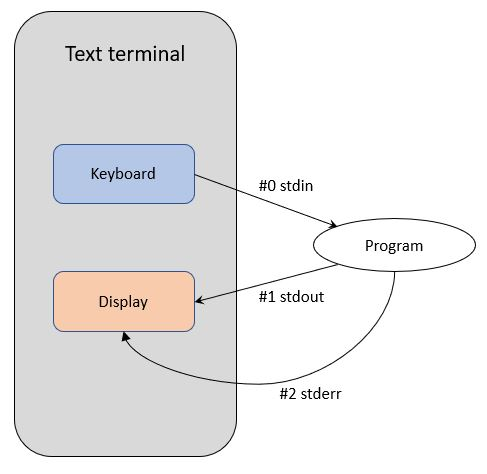
\includegraphics{streams}
  \caption{Standard Streams}
  \labfig{streams}
\end{marginfigure}

However, sometimes a process may need to take input from a file or
send output to a file. When this is required, the standard stream is
mapped to a file. This is known as \textbf{redirection}.

To maintain which file or resource is mapped to which stream, the
operating system maintains a table known as the \textbf{file descriptor
table}. The file descriptor table is a table that maps the file
descriptors to the files or resources.

\begin{definition}[File Descriptor]
  A \textbf{file descriptor} is a process-unique identifier that the
  operating system assigns to a file or resource.
  The file descriptor is an integer that is used to identify
  the file or resource.
\end{definition}

The default file descriptors are:

\begin{enumerate}
  \item \textbf{Standard Input (stdin)}: File descriptor 0
  \item \textbf{Standard Output (stdout)}: File descriptor 1
  \item \textbf{Standard Error (stderr)}: File descriptor 2
\end{enumerate}

In the traditional implementation of Unix, file descriptors index
into a per-process file descriptor table maintained by the kernel,
that in turn indexes into a system-wide table of files opened by
all processes, called the file table. This table records the mode
with which the file (or other resource) has been opened: for
reading, writing, appending, and possibly other modes. It also indexes
into a third table called the inode table
\sidenote{
  We have covered inodes and inode tables in detail in the
  \refch{basic} chapter.
}
that describes the actual
underlying files. To perform input or output, the process passes
the file descriptor to the kernel through a system call, and the
kernel will access the file on behalf of the process. The process
does not have direct access to the file or inode tables.

\begin{marginfigure}
  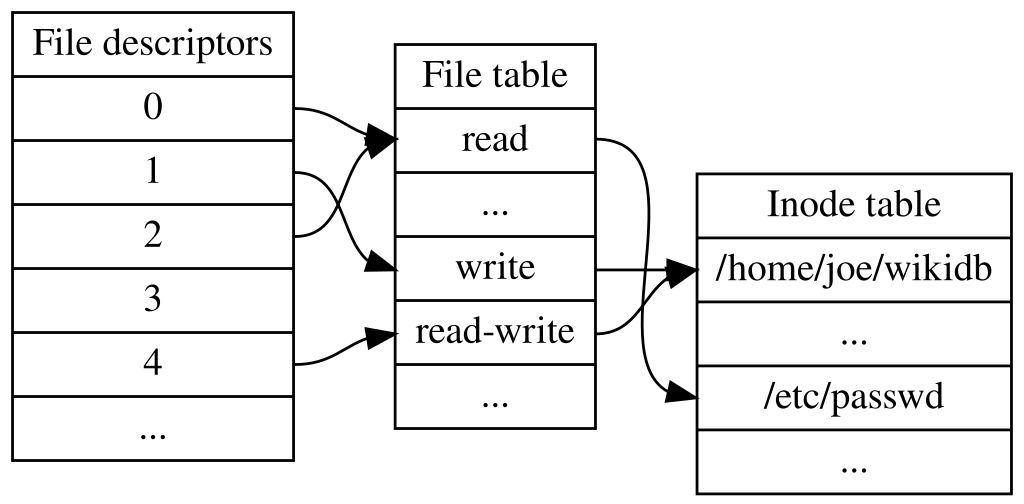
\includegraphics{fdtable}
  \caption{File Descriptor Table}
  \labfig{fdtable}
\end{marginfigure}

The file descriptors of a process can be inspected in the \lstinline|/proc|
directory. The \lstinline|/proc| directory is a pseudo-filesystem that
provides an interface to kernel data structures. The \lstinline|/proc/PID/fd|
directory contains the file descriptors of the process with the PID.

Most GNU core utilities that accept a file as an argument will also
work without the argument and will read from the standard input.
This behaviour lets us chain commands together using pipes easily
without any explicit file handling.

\begin{lstlisting}[language=bash]
$ cat
hello
hello
This command is repeating the input
This command is repeating the input
Press Ctrl+D to exit
Press Ctrl+D to exit
\end{lstlisting}

The \lstinline|cat| command is usually used to print the contents of one
or more files. However, when no file is provided, it reads from the
standard input. In this case, the standard input is the keyboard.
This is very useful when we want to repeat the input or when we want
to read from the standard input.

\begin{qs}
  Can we also use cat to write to a file?
\end{qs}

\begin{ans}
  Yes, we can use the \lstinline|cat| command to write to a file. When
  no file is provided, the \lstinline|cat| command reads from the standard
  input. So the input will be printed back to the standard output.
  However, if we can somehow change the standard output to a file,
  then the input will be written to the file.
\end{ans}

\section{Redirection}

Redirection is the process of changing the standard streams of a process.
This is done by the shell before the process is executed. The shell
uses the \lstinline|<|, \lstinline|>|, and \lstinline|2>| operators to redirect
the standard input, standard output, and standard error streams of a
process.

As the shell is responsible for redirection, the process is not aware
of the redirection. The process reads from or writes to the file descriptor
it is given by the shell. The process does not know whether the file
descriptor is a file, a terminal, or a pipe.

However, there are ways for a process to guess whether the file descriptor
is a terminal or a file. This is done by using the \lstinline|isatty()|
function. The \lstinline|isatty()| function returns \lstinline|1| if the file
descriptor is a terminal, and \lstinline|0| if the file descriptor is a file.

\subsection{Standard Output Redirection}

The standard output of a process can be redirected to a file using the
\lstinline|>| operator. Observe the following example.

\begin{lstlisting}[language=bash]
$ date > date.txt
$ cat date.txt
Thu Jul  4 07:37:27 AM IST 2024
\end{lstlisting}

Here, the output of the \lstinline|date| command is redirected to the file
\lstinline|date.txt|. The \lstinline|cat| command is then used to print the
contents of the file \lstinline|date.txt|.

The process did not print the output to the terminal. Instead, the shell
changed the standard output of the process to the file \lstinline|date.txt|.

We can also use redirection to create a file. If the file does not exist,
the shell will create the file. If the file exists, the shell will truncate
the file.

\begin{lstlisting}[language=bash]
$ > empty.txt
\end{lstlisting}

This command creates an empty file \lstinline|empty.txt|. The \lstinline|>|
operator is used to redirect the output of the command to the file
\lstinline|empty.txt|. Since there is no output, the file is empty.

We can also use redirection along with the \lstinline|echo| command to
create a file with some content.

\begin{lstlisting}[language=bash]
$ echo "hello" > hello.txt
$ cat hello.txt
hello
\end{lstlisting}

Here, the output of the \lstinline|echo| command is redirected to the file
\lstinline|hello.txt|. The \lstinline|cat| command is then used to print the
contents of the file \lstinline|hello.txt|.

Recall that the cat command will read from the standard input if no
file is provided. We can use this to create a file with the input from
the standard input.

\begin{lstlisting}[language=bash]
$ cat > file.txt
hello, this is input typed from the keyboard
I am typing more input
all this is being written to the file
to stop, press Ctrl+D
$ cat file.txt
hello, this is input typed from the keyboard
I am typing more input
all this is being written to the file
to stop, press Ctrl+D
\end{lstlisting}

It is important to note that the process of creating the file if it
does not exist, and truncating the file if it exists, along with redirecting
the output, is done by the shell, not the process. All of this is done
before the process is executed. This creates an interesting exemplar when
using redirection with the \lstinline|ls| command.

\textbf{Output contains output}

\begin{lstlisting}[language=bash]
$ ls
hello
$ ls > output.txt
$ cat output.txt
hello
output.txt
\end{lstlisting}

Since the file is created even before the process is executed, the file
is also a part of the output of the \lstinline|ls| command. This is why the
file \lstinline|output.txt| is also printed by the \lstinline|cat| command.

\textbf{Output format changes}

Another interesting example using the \lstinline|ls| command is when the
directory contains more than one file.
The output of \lstinline|ls| is usually formatted to fit the terminal.
However, when the output is redirected to a file, the output is not
in a column format. Instead, each file is printed on a new line.

\begin{lstlisting}[language=bash]
$ ls
hello  output.txt
$ ls > output.txt
$ cat output.txt
hello
output.txt
\end{lstlisting}

Observe that the output of the \lstinline|ls| command is not in a column
when redirected to a file. But how does \lstinline|ls| know that the output
is not a terminal? It uses the file descriptor to guess whether the
output is a terminal or a file. If the file descriptor is a terminal,
then the output is formatted to fit the terminal. If the file descriptor
is a file, then the output is not formatted.

However, we can always force the output to be single-column using the
\lstinline|-1| option.

\begin{lstlisting}[language=bash]
$ ls -1
hello
output.txt
\end{lstlisting}

This behaviour is not limited to the \lstinline|ls| command. Most commands
usually strip out the formatting when the output is redirected to a file.

If you are using a terminal that supports ANSI escape codes
\sidenote{
  ANSI escape codes are special sequences of characters that are used
  to control the terminal. For example, to change the color of the text,
  the ANSI escape code \lstinline|\[31m| is used.
  Similarly other ANSI escape codes are used to change the text style,
  and the position and state of the cursor.
}
, you can
use the \lstinline|ls| command with the \lstinline|--color=auto| option to
get colored output. However, when the output is redirected to a file,
the ANSI escape codes are not printed. This is because the ANSI escape
codes are not printable characters. They are control characters that
tell the terminal to change the color of the text.

\textbf{Output and Input from same file}

If you try to redirect the output of a command to a file, and then
also try to read from the same file, you will get an empty file.
This is because the file is truncated before the command is executed.

\begin{lstlisting}[language=bash]
$ echo "hello" > output.txt
$ cat output.txt
hello
$ cat output.txt > output.txt
$ cat output.txt
$
\end{lstlisting}

\begin{remark}
  Although we can simply use \lstinline|>| to redirect the output to a file,
  the full syntax is \lstinline|1>|. This is because the file descriptor
  for the standard output is 1. The \lstinline|1>| is used to redirect
  the standard output to a file. However, since the standard output
  is the default output, we can omit the \lstinline|1| and use only \lstinline|>|.
\end{remark}

\subsection{Standard Error Redirection}

The standard error of a process can be redirected to a file using the
\lstinline|2>| operator. Observe the following example.

\begin{lstlisting}[language=bash]
$ ls /nonexistant 2> error.txt
$ cat error.txt
ls: cannot access '/nonexistant': No such file or directory
\end{lstlisting}

Here, the error message of the \lstinline|ls| command is redirected to the
file \lstinline|error.txt|. The \lstinline|cat| command is then used to print
the contents of the file \lstinline|error.txt|.

It is important to realise that each process has two streams to output
to, the standard output and the standard error. The standard output is
usually used to print the output of the process, while the standard error
is used to print the error messages.

This helps us differentiate between the output and the error messages.
Also, if the output of a process is redirected to a file, the error
will still be printed to the terminal. This is because the standard
error is not redirected to the file. This makes debugging easier, as
the error messages are not lost.

\begin{lstlisting}[language=bash]
$ ls -d /home /nonexistant > output.txt
ls: cannot access '/nonexistant': No such file or directory
$ cat output.txt
/home
\end{lstlisting}

Here, the output of the \lstinline|ls| command is redirected to the file
\lstinline|output.txt|. However, the error message is still printed to
the terminal.

We can redirect both the standard output and the standard error to
files using the \lstinline|>| and \lstinline|2>| operators.

\begin{lstlisting}[language=bash]
$ ls -d /home /nonexistant > output.txt 2> error.txt
$ cat output.txt
/home
$ cat error.txt
ls: cannot access '/nonexistant': No such file or directory
\end{lstlisting}

\textbf{Redirecting both streams to the same file}

Lets try to redirect both the standard output and the standard error
to the same file.

\begin{lstlisting}[language=bash]
$ ls -d /home /nonexistant > output.txt 2> output.txt
$ cat output.txt
/home
nnot access '/nonexistant': No such file or directory
\end{lstlisting}

Why did the error message get mangled? This is because the shell
truncates the file before the process is executed. So the error
is written to the file, and then the output message is written to
the same file, overwriting the error partially.
Observe that only the first six characters of the
error message are mangled, the same size of the output.
\sidenote{
  The output message is \lstinline|/home|, followed by a newline character.
  This makes the output message 6 characters long.
  The shell first writes the error message to the file (because that is
  printed first by the ls command), and then overwrites the first 6 bytes
  of the file with the output message. Since the 6th byte is a newline
  character, it looks like there are two lines in the file.
}

The correct way to redirect both the standard output and the standard
error to the same file is to use the \lstinline|2>\&1| operator.
This means that the standard error is redirected to the standard output.
Here, the \lstinline|1| is the file descriptor for the standard output.
The \lstinline|&| is used to tell the shell that the \lstinline|1| is a file
descriptor, not a file.

\begin{lstlisting}[language=bash]
$ ls -d /home /nonexistant > output.txt 2>&1
$ cat output.txt
ls: cannot access '/nonexistant': No such file or directory
/home
\end{lstlisting}

However, the order is important. The \lstinline|2>\&1| operator should
be placed at the end of the command. If it is placed at the beginning,
then the standard error will be redirected to the standard output, which,
at that point, is the terminal. Then the standard output will be redirected
to the file. Thus, only the standard output will be redirected to the file.

\begin{lstlisting}[language=bash]
$ ls -d /home /nonexistant 2>&1 > output.txt
ls: cannot access '/nonexistant': No such file or directory
$ cat output.txt
/home
\end{lstlisting}

\subsection{Appending to a File}

The \lstinline|>| operator is used to redirect the output to a file. If the
file does not exist, the shell will create the file. If the file exists,
the shell will truncate the file. However, if we want to append the output
to the file, we can use the \lstinline|>>| operator.

\begin{lstlisting}[language=bash]
$ echo "hello" > hello.txt
$ cat hello.txt
hello
$ echo "world" > hello.txt
$ cat hello.txt
world
$ echo "hello" > hello.txt
$ echo "world" >> hello.txt
$ cat hello.txt
hello
world
\end{lstlisting}

Observe that the \lstinline|>| operator truncates the file, while the
\lstinline|>>| operator appends to the file.

We can also append the standard error to a file using the \lstinline|2>>|

\begin{lstlisting}[language=bash]
$ ls /nonexistant 2> error.txt
$ cat error.txt
ls: cannot access '/nonexistant': No such file or directory
$ daet 2>> error.txt
$ cat error.txt
ls: cannot access '/nonexistant': No such file or directory
bash: daet: command not found
\end{lstlisting}

This is useful when we want to append the error messages to a file,
like in a log file.

\textbf{Circular Redirection}

If we try to redirect the output of a command to the same file that
we are reading from, we will get an empty file. However, if we append
the output to the file, we will get an infinite loop of the output.
This should not be done, as it will fill up the disk space.
However, GNU core utilities \lstinline|cat| is smart enough to detect
this and will not read from the file.

\begin{lstlisting}[language=bash]
$ echo hello > hello
$ cat hello >> hello
cat: hello: input file is output file
$ cat < hello > hello
cat: -: input file is output file
\end{lstlisting}

However, it can still be tricked by using a pipe.
\sidenote{
  We will cover pipes in the next section.
}

\begin{lstlisting}[language=bash]
$ echo hello > hello
$ cat hello | cat >> hello
$ cat hello
hello
hello
\end{lstlisting}

Here we dont get into an infinite loop because the first cat command
reads from the file and writes to the pipe. The second cat command
reads from the pipe and writes to the file. Since the file is not
read from and written to at the same time, we dont get into an infinite
loop.

However, BSD utilities like \lstinline|cat| do not have this check, thus
giving the same input and output file will result in an infinite loop.

\subsection{Standard Input Redirection}

The standard input of a process can be redirected from a file using
the \lstinline|<| operator. Although most commands accept a filename
in the argument to read from, so we can directly provide the file
in the argument. However, some commands do not accept a filename
and only read from the standard input. In such cases, we can use
the \lstinline|<| operator to redirect the standard input from a file.

\begin{lstlisting}[language=bash]
$ wc < ~/.bashrc
  340  1255 11238
\end{lstlisting}

Although the \lstinline|wc| command accepts a filename as an argument,
we can also redirect the standard input from a file using the \lstinline|<|
to the command. However, now the output of the \lstinline|wc| command
is different than when we provide the filename as an argument.

\begin{lstlisting}[language=bash]
$ wc ~/.bashrc
  340  1255 11238 /home/sayan/.bashrc
\end{lstlisting}

When we provide the filename as an argument, the \lstinline|wc| command
prints the number of lines, words, and characters in the file, followed
by the filename. However, when we redirect the standard input from a
file, the \lstinline|wc| command prints only the number of lines, words,
and characters in the file. This is because it does not know that the
input is coming from a file. For \lstinline|wc|, the input is just a stream
coming from the standard input.

\begin{lstlisting}[language=bash]
$ wc
Hello, this is input from the keyboard
I can simply type more input here
All of this is taken as standard input
by wc command
Stop by pressing Ctrl+D
      5      29     150
\end{lstlisting}

Another example where giving filename is not possible is the \lstinline|read|
command. The \lstinline|read| command reads a line from the standard input
and assigns it to a variable. The \lstinline|read| command does not accept
a filename as an argument. So we have to use the \lstinline|<| operator to
redirect the standard input from a file.

\begin{lstlisting}[language=bash]
$ read myline < /etc/hostname
$ echo $myline
rex
\end{lstlisting}

Here, the \lstinline|read| command reads a line from the file \lstinline|/etc/hostname|
and assigns it to the variable \lstinline|myline|. The \lstinline|echo| command
is then used to print the value of the variable \lstinline|myline|.
To access the value of the variable, we use the \lstinline|$| operator.
\sidenote{
  This will be covered in depth in the \refch{variables} chapter.
}

\subsection{Here Documents}

A \textbf{here document} is a way to provide input to a command without
using a file. The input is provided directly in the command itself.
This is done by using the \lstinline|<<| operator followed by a delimiter.

\begin{lstlisting}[language=bash]
$ wc <<EOF
This is acting like a file
however the input is directly provided
to the shell or the script
this is mostly used in scripts
we can use any delimiter instead of EOF
to stop, type the delimiter on a new line
EOF
      6      41     206
\end{lstlisting}

We can optionally provide a hyphen \lstinline|-| after the \lstinline|<<|
to ignore leading tabs. This is useful when the here document is
indented.

\begin{lstlisting}[language=bash]
$ cat <<EOF
> hello
>     this is space
>       this is tab
> EOF
hello
    this is space
        this is tab
$ cat <<-EOF
hello
    this is space
        this is tab
EOF
hello
    this is space
this is tab
\end{lstlisting}

The delimiter can be any string. However, it is common to use \lstinline|EOF|
as the delimiter. The delimiter should be on a new line.

\begin{lstlisting}[language=bash]
$ wc <<END
If I want to have
EOF
as part of the input
then I can simply change the delimiter
END
      4      18      82
\end{lstlisting}

Here-documents also support variable expansion. The shell will expand
the variables before passing the input to the command. Thus
it is really useful in scripts if we want to provide a template
which is filled with the values of the variables.

\begin{lstlisting}[language=bash]
$ name="Sayan"
$ cat <<EOF
Hello, $name
This is a here document
EOF
Hello, Sayan
This is a here document
\end{lstlisting}

\subsection{Here Strings}

A \textbf{here string} is a way to provide input to a command without
using a file. The input is provided directly in the command itself.
This is done by using the \lstinline|<<<| operator followed by the input.
It is very similar to the here document, but the input is provided
in a single line. Due to this, a delimiter is not required.

\begin{lstlisting}[language=bash]
$ wc <<< "This is a here string"
      1       5      22
\end{lstlisting}

It can also perform variable expansion.

\begin{lstlisting}[language=bash]
$ cat <<< "Hello, $USER"
Hello, sayan
\end{lstlisting}

\begin{remark}
  Both heredocs and herestrings are simply syntactic sugar. They are
  similar to using echo and piping the output to a command. However,
  it requires one less process to be executed.
\end{remark}

\section{Pipes}

\begin{marginfigure}
  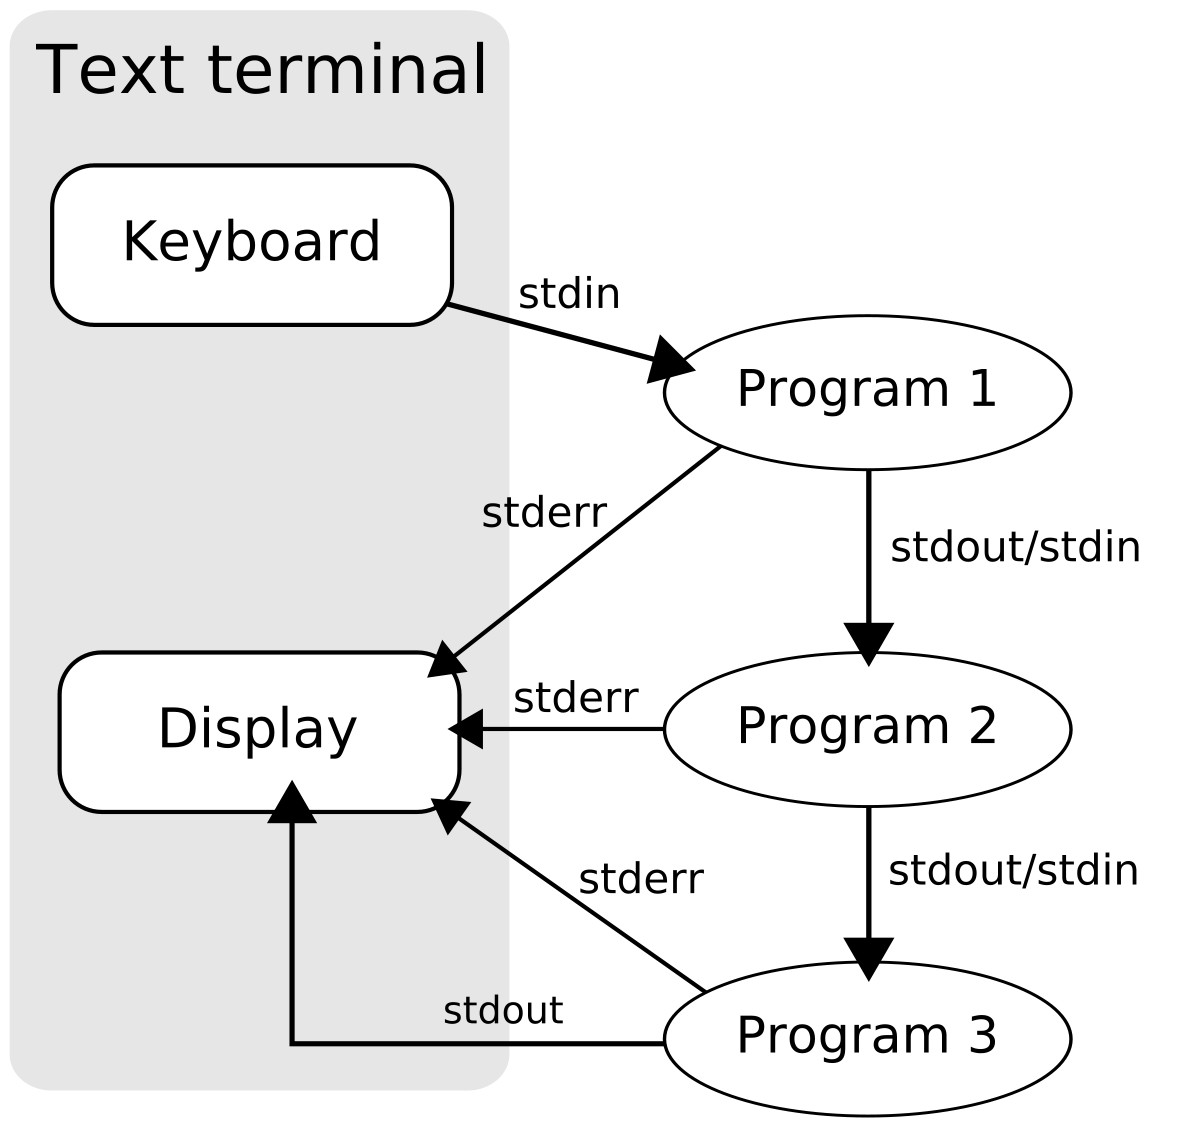
\includegraphics{pipes}
  \caption{Pipes}
  \labfig{pipes}
\end{marginfigure}

Pipes are the holy grail of Unix-like operating systems.
They are the most important concept to understand
in Unix-like operating systems.

\begin{definition}[Pipe]
  A \textbf{pipe} is a way to connect the standard output of one process
  to the standard input of another process. This is done by using the
  \lstinline||| operator.
\end{definition}

Think of the shell as a factory, and the commands as machines in the
factory. Pipes are like conveyor belts that connect the machines.
It would be a pain if we had to manually collect the produce of one
machine and then feed it to the next machine. Conveyors make it easy
by automatically taking the output of one machine and feeding it to
the next machine.

Pipes are the same, but for processes in shell.

\begin{lstlisting}[language=bash]
$ date
Thu Jul  4 09:05:30 AM IST 2024
$ date | wc
      1       7      32
\end{lstlisting}

\subsection{UNIX Philosophy}

Each process simply takes the standard input and writes to the standard
output. How those streams are connected is not the concern of the process.
This way of simply doing one thing and doing it well is the Unix philosophy
\sidenote{
The Unix philosophy, originated by Ken Thompson,
is a set of cultural norms and philosophical approaches
to minimalist, modular software development.
It is based on the experience of leading developers
of the Unix operating system.
Read more
\href{https://en.wikipedia.org/wiki/Unix\_philosophy}{online}.
}
which says that each program should do one thing and do it well.
Each process should take input from the standard input and write to
the standard output. The output of the process should be easy to
parse by another process. The output of the process should not contain
unnecessary information. This makes it easy to chain commands together
using pipes.

\subsection{Multiple Pipes}

There is no limit to the number of pipes that can be chained together.
It simply means that the output of one process is fed to the input
of the next process. This simple but powerful construct lets the user
do any and all kinds of data processing.

Imagine you have a file which contains a lot of words, you want to
find which word is present the most number of times. You can either
write a program in C or Python, etc., or you can use the power of
pipes to do it in a single line using simple GNU coreutils.

I have a file \lstinline|alice\_in\_wonderland.txt| which contains the
entire text of the book Alice in Wonderland. I want to find the words
that are present the most number of times.

There are some basic preprocessing you would do even if you were writing
a program. You would convert all the words to lowercase, and remove
any punctuation. This can be done using the \lstinline|tr| command.
Then you would split the text into each word. This can be done using
the \lstinline|tr| command. Then you would find the count of each word.
There are two ways of doing this, either you can use a dictionary
\sidenote{
  A dictionary in python is a hash map. It is a data structure that
  maps keys to values. The keys are unique, and the values can be
  accessed using the keys. It has amortized constant time complexity
  for insertion, deletion, and lookup.
}
to store the frequency of each word, and increase it as you iterate
over the entire text once. Or you can first sort the words, then
simply count the number of times each word is repeated. Since repeated
words would always be consecutive, you can simply count the number
of repeated words without having to store the frequency of each word.
This can be done using the \lstinline|sort| and \lstinline|uniq| commands.
Finally, you would sort the words based on the frequency and print
the top 10 words. This can be done using the \lstinline|sort| and \lstinline|head|
commands.

Lets see how we actually do this using pipes.

\begin{lstlisting}[language=bash]
$ ls alice_in_wonderland.txt
alice_in_wonderland.txt
$ tr 'A-Z' 'a-z' < alice_in_wonderland.txt  | tr -cd 'a-z ' | tr ' ' '\n' | grep . | sort | uniq -c | sort -nr | head
   1442 the
    713 and
    647 to
    558 a
    472 she
    463 it
    455 of
    435 said
    357 i
    348 alice
\end{lstlisting}

Let's go over each command one by one and see what it does.

\textbf{tr 'A-Z' 'a-z'}

\lstinline|tr| is a command that translates characters. The first argument
is the set of characters to be translated, and the second argument is
the set of characters to translate to. Here, we are translating all
uppercase letters to lowercase.
This command converts all uppercase letters to lowercase. This is done
to make the words case-insensitive.

\begin{lstlisting}[language=bash]
$ tr 'A-Z' 'a-z' < alice_in_wonderland.txt  | head -n20
alice's adventures in wonderland

                alice's adventures in wonderland

                          lewis carroll

               the millennium fulcrum edition 3.0




                            chapter i

                      down the rabbit-hole


  alice was beginning to get very tired of sitting by her sister
on the bank, and of having nothing to do:  once or twice she had
peeped into the book her sister was reading, but it had no
pictures or conversations in it, `and what is the use of a book,'
\end{lstlisting}

\begin{remark}
  Since the text is really big, I am  going to filter all the
  intermediate outputs also through the \lstinline|head| command.
\end{remark}

\textbf{tr -cd 'a-z '}

The \lstinline|-c| option is used to complement the set of characters.
The \lstinline|-d| option is used to delete the characters. Here, we are
telling the \lstinline|tr| command to delete all characters except lowercase
letters and spaces. This is done to remove all punctuation and special
characters. Observe the difference in output now.

\begin{lstlisting}[language=bash]
$ tr 'A-Z' 'a-z' < alice_in_wonderland.txt  | tr -cd 'a-z ' | head -c500
alices adventures in wonderland                alices adventures in wonderland                          lewis carroll               the millennium fulcrum edition                             chapter i                      down the rabbithole  alice was beginning to get very tired of sitting by her sisteron the bank and of having nothing to do  once or twice she hadpeeped into the book her sister was reading but it had nopictures or conversations in it and what is the use of a bookthought alice w
\end{lstlisting}

\begin{remark}
  After we have removed all the punctuation, the text is now
  only a single line. This is because we have removed all the
  characters, including the newline characters.
  Thus to restrict the output, I am using the \lstinline|head -c500|
  instead of \lstinline|head -n20|.
\end{remark}

\textbf{tr ' ' '\textbackslash n'}

The \lstinline|tr| command is used to translate characters. Here, we are
translating spaces to newline characters. This is done to split the
text into words. We are doing this so that each word is on a new line.
This is helpful as the sort and uniq commands work on lines.

\begin{lstlisting}[language=bash]
$ tr 'A-Z' 'a-z' < alice_in_wonderland.txt  | tr -cd 'a-z ' | tr ' ' '\n' | head -20
alices
adventures
in
wonderland















alices
\end{lstlisting}

\textbf{grep .}

Now we have each word on a new line.
But observe that there are many empty lines.
This is because of the multiple spaces between words and spaces around
punctuation. We can remove these empty lines using the \lstinline|grep .|
command.
\sidenote{
  We will learn more about regular expressions in the \refch{regex} chapter.
}

\begin{lstlisting}[language=bash]
$ tr 'A-Z' 'a-z' < alice_in_wonderland.txt  | tr -cd 'a-z ' | tr ' ' '\n' | grep . | head -20
alices
adventures
in
wonderland
alices
adventures
in
wonderland
lewis
carroll
the
millennium
fulcrum
edition
chapter
i
down
the
rabbithole
alice
\end{lstlisting}

Now we are almost there. We have each word on a new line. Now we can
pass this entire stream of words to the \lstinline|sort| command, this
will sort the words.

\textbf{sort}

Sort by default sorts the words in lexicographical order. This is
useful as repeated words would be consecutive. This is important
as the \lstinline|uniq| command only works on consecutive lines only.

\begin{lstlisting}[language=bash]
$ tr 'A-Z' 'a-z' < alice_in_wonderland.txt  | tr -cd 'a-z ' | tr ' ' '\n' | grep . | sort | head -20
a
a
a
a
a
a
a
a
a
a
a
a
a
a
a
a
a
a
a
a
\end{lstlisting}

If you run the command yourself without the \lstinline|head| command, you
can see that the words are sorted. The repeated words are consecutive.
In the above output we can see that the word \lstinline|a| is repeated
many times. Now we can use the \lstinline|uniq| command to count the
number of times each word is repeated.

\textbf{uniq -c}

The \lstinline|uniq| command is used to remove consecutive duplicate lines.
However, it also can count the number of times each line is repeated
using the \lstinline|-c| option.

\begin{lstlisting}[language=bash]
$ tr 'A-Z' 'a-z' < alice_in_wonderland.txt  | tr -cd 'a-z ' | tr ' ' '\n' | grep . | sort | uniq -c | head -20
    558 a
      1 abarrowful
      1 abat
      1 abidefigures
      1 able
     79 about
      1 aboutamong
      1 aboutand
      1 aboutby
      3 abouther
      3 aboutit
      1 aboutthis
      1 abouttrying
      2 above
      1 abranch
      1 absenceand
      2 absurd
      1 acceptance
      2 accident
      1 accidentally
\end{lstlisting}

Great! Now we have the count of each word. However, the words are
still sorted by the word. We want to sort the words by the count
of the word. This can be done using the \lstinline|sort| command.

\textbf{sort -nr}

Sort by default sorts in lexicographical order. However, we want to
sort by the count of the word. The \lstinline|-n| option is used to sort
the lines numerically. The \lstinline|-r| option is used to sort in
reverse order.

\begin{exercise}
  Try to run the same command without the \lstinline|-n| option.
  Observe how the sorting makes sense alphabetically, but not
  numerically.
\end{exercise}

\begin{lstlisting}[language=bash]
$ tr 'A-Z' 'a-z' < alice_in_wonderland.txt  | tr -cd 'a-z ' | tr ' ' '\n' | grep . | sort | uniq -c | sort -nr | head -20
   1442 the
    713 and
    647 to
    558 a
    472 she
    463 it
    455 of
    435 said
    357 i
    348 alice
    332 you
    332 in
    313 was
    241 that
    237 as
    202 her
    190 at
    169 on
    161 all
    158 with
\end{lstlisting}

Finally, we have the top 20 words in the file \lstinline|alice\_in\_wonderland.txt|
along with the count of each word.

Although the above command is a single line
\sidenote{
  Such commands are called one-liners.
}
, it is doing a lot of
processing. Still, it is very readable. This is the power of pipes.

\begin{remark}
  Usually, when we come across such one-liners, it may initially
  seem to complicated to understand. The key to understanding such
  one-liners is to break them down into smaller parts and understand
  them one component at a time from left to right. Feel free to
  execute each command separately and observe the output like we
  did above.
\end{remark}

\subsection{Piping Standard Error}

Pipes are used to connect the standard output of one process to the
standard input of another process. However, the standard error is not
connected and remains mapped to the terminal. This is because the
standard error is a separate stream from the standard output.

However, we can connect the standard error to the standard input of
another process using the \lstinline|2>\&1| operator. This is useful when
we want to process the error messages of a command.

\begin{lstlisting}[language=bash]
$ ls -d /home /nonexistant | wc
"/nonexistant": No such file or directory (os error 2)
      1       1       6
$ ls -d /home /nonexistant 2>&1 | wc
      2      10      61
\end{lstlisting}

This is same as redirecting both the streams to a single file as
demostrated earlier.

However, there is a shorter way to do this using the \lstinline||\&|
syntactic sugar.

\begin{lstlisting}[language=bash]
$ ls -d /home /nonexistant |& wc
      2      10      61
\end{lstlisting}

This does the exact same thing as \lstinline|2>\&1| followed by the pipe.

\subsection{Piping to and From Special Files}

As we discussed earlier, there are some special files in the \lstinline|/dev|
directory.

\textbf{/dev/null}

The \lstinline|/dev/null| file is a special file that discards all the data
that is written to it. It is like a black hole. All the data that is
not needed can be written to this file. Usually errors are written to
the \lstinline|/dev/null| file.

\begin{lstlisting}[language=bash]
$ ls -d /nonexistant /home 2> /dev/null
/home
\end{lstlisting}

The error is not actually stored in any file, thus the storage
space is not wasted.

\textbf{/dev/zero}

The \lstinline|/dev/zero| file is a special file that provides an infinite
stream of null bytes. This is useful when you want to provide an infinite
stream of data to a process.

\begin{lstlisting}[language=bash]
$ head -c1024 /dev/zero > zero.txt
$ ls -lh zero.txt
-rw-r--r-- 1 sayan sayan 1.0K Jul  4 15:04 zero.txt
\end{lstlisting}

Here we are taking the first 1024 bytes from the \lstinline|/dev/zero|
and writing it to the file \lstinline|zero.txt|. The file \lstinline|zero.txt|
is 1.0K in size. This is because the \lstinline|/dev/zero| file provides
an infinite stream of null bytes, of which $1024$ bytes are taken.

\begin{warn}
  Make sure to always use \lstinline|head| or any other limiter when
  working with \lstinline|/dev/zero| or \lstinline|/dev/random| as they
  are infinite streams. Forgetting this can lead to the disk being
  filled up. Head with the default parameter will also not work,
  since it depends on presence of newline characters, which is
  not there in an infinite stream of zeros. That is why we are
  using a byte count limiter using the \lstinline|-c| option.
  If you forget to add the limiter, you can press \lstinline|Ctrl+C|
  as quickly as possible to stop the process and then remove the
  file using \lstinline|rm|.
\end{warn}

\textbf{/dev/random and /dev/urandom}

The \lstinline|/dev/random| and \lstinline|/dev/urandom| files are special
files that are infinite suppliers of random bytes. The \lstinline|/dev/random|
file is a blocking random number generator. This means that it will
block if there is not enough entropy. The \lstinline|/dev/urandom| file
is a non-blocking random number generator. This means that it will
not block even if there is not enough entropy. Both can be used to
generate random numbers.

\begin{lstlisting}[language=bash]
$ head -c1024 /dev/random > random.txt
$ ls -lh random.txt
-rw-r--r-- 1 sayan sayan 1.0K Jul  4 15:04 random.txt
\end{lstlisting}

Observe that here too the file is of size 1.0K. This is because we
are still taking only the first 1024 bytes from the infinite stream
of random bytes. However, if we gzip the data, we can see that the
zeros file is much smaller than the random file.

\begin{lstlisting}[language=bash]
$ gzip random.txt zero.txt
$ ls -lh random.txt.gz zero.txt.gz
-rw-r--r-- 1 sayan sayan 1.1K Jul  4 15:11 random.txt.gz
-rw-r--r-- 1 sayan sayan   38 Jul  4 15:10 zero.txt.gz
\end{lstlisting}

The random file is 1.1K in size, while the zero file is only 38 bytes
in size. This is because the random file has more entropy and thus
cannot be compressed as much as the zero file.

\subsection{Named Pipes}

A \textbf{named pipe} is a special file that provides a way to connect
the standard output of one process to the standard input of another
process. This is done by creating a special file in the filesystem.
We have already covered named pipes in the \refch{basic} chapter.

Although a pipe is faster than a named pipe, a named pipe can be used
to connect processes that are not started at the same time or from
the same shell. This is because a named pipe is a file in the filesystem
and can be accessed by any process that has the permission to access
the file.

Try out the following example. First create a named pipe using the
\lstinline|mkfifo| command.

\begin{lstlisting}[language=bash]
$ mkfifo pipe1
\end{lstlisting}

Then run two processes, one that writes to the named pipe, another
that reads from the named pipe. The order of running the processes
is not important.

\textbf{Terminal 1:}
\begin{lstlisting}[language=bash]
$ cat /etc/profile > pipe1
\end{lstlisting}

\textbf{Terminal 2:}
\begin{lstlisting}[language=bash]
$ wc pipe1
     47     146     993 pipe1
\end{lstlisting}

\begin{exercise}
  After you have created the named pipe,
  try changing the order of running the other two processes.
  Observe that whatever is run first will wait for
  the other process to start.
  This is because a named pipe is not storing the data piped to it
  in the filesystem. It is simply a buffer in the memory.
\end{exercise}

A named pipe is more useful over regular files when two processes
want to communicate with each other. This is because a named pipe
is

\begin{enumerate}
  \item Faster than a regular file as it does not store the data in
    the file system.
  \item Independent of the order of launching the processes.
    The reader can be launched first and it will still wait for
    the writer to send the data.
  \item Works concurrently. The writer does not need to be done
    writing the entire data before the reader can start reading.
    The reader can start as soon as the writer starts writing.
    The faster process will simply block until the slower process
    catches up.
\end{enumerate}

To demonstrate the last point, try running the following commands.

Ensure that a named pipe is created.

\textbf{Terminal 1:}

\begin{lstlisting}[language=bash]
$ grep linux pipe1
\end{lstlisting}

This process is looking for lines containing the word \lstinline|linux|
in the file \lstinline|pipe1|. Initially it will simply block.
Grep is a command that does not wait for the entire file to be read.
It starts printing output as soon as a line containing the pattern
is read.

\textbf{Terminal 2:}
\begin{lstlisting}[language=bash]
$ tree / > pipe1
\end{lstlisting}

This command is attempting to list out each and every file on
the filesystem. This takes a lot of time. However, since
we are using a named pipe, the \lstinline|grep| command will start
running as soon as the first line is written to the pipe.

You can now observe the first terminal will start printing
some lines containing the word \lstinline|linux| as soon as the
second terminal starts writing to the pipe.

Now try the same with a regular file.

\begin{lstlisting}[language=bash]
$ touch file1 # ensure its a normal file
$ tree / > file1
$ grep linux file1
\end{lstlisting}

Since this is a regular file, we cannot start reading from the
file before the entire file is written. If we do that, the grep
command will quit as soon as it catches up with the writer, it
will not block and wait.

Observe that to start getting output on the screen takes a lot
longer in this method. Not to mention the disk space wasted
due to this.

\begin{remark}
  Remember that when we use redirection (\lstinline|>|) to write to a file,
  the shell truncates the file. But when we use a named pipe, the shell
  knows that the file is a named pipe and does not truncate the file.
\end{remark}

\subsection{Tee Command}

The \lstinline|tee| command is a command that reads from the standard
standard input and writes to the standard output and to a file.
It is very useful when you want to save the output of a command
but also want to see the output on the terminal.

\begin{lstlisting}[language=bash]
$ ls -d /home /nonexistant | tee output.txt
ls: cannot access '/nonexistant': No such file or directory
/home
$ cat output.txt
/home
\end{lstlisting}

Observe that only the standard output is written to the file, and
not the standard error. This is because pipes only connect the
standard output to the standard input of the next command, and the
standard error remains mapped to the terminal.

Thus in the above output, although it may look like that both
the standard output and the standard error are written to the
terminal by the same command, it is not so.

The standard error of the ls command remains mapped to the terminal,
and thus gets printed directly, whereas the standard output is
redirected to the standard input of the tee command, which then
prints that to the standard output (and also writes it to the file).

You can also mention multiple files to write to.

\begin{lstlisting}[language=bash]
$ ls -d /home | tee output1.txt output2.txt
$ cat output1.txt
/home
$ cat output2.txt
/home
$ diff output1.txt output2.txt
$
\end{lstlisting}

\begin{remark}
  The \lstinline|diff| command is used to compare two files. If the
  files are the same, then the \lstinline|diff| command will not print
  anything. If the files are different, then the \lstinline|diff| command
  will print the lines that are different.
\end{remark}

We can also append to the file using the \lstinline|-a| option.

\begin{lstlisting}[language=bash]
$ ls -d /home | tee output.txt
$ ls -d /etc | tee -a output.txt
$ cat output.txt
/home
/etc
\end{lstlisting}

\section{Command Substitution}

We have already seen that we can run multiple commands in a subshell
in bash by enclosing them in parentheses.

\begin{lstlisting}[language=bash]
$ (whoami; date)
sayan
Thu Jul  4 09:05:30 AM IST 2024
\end{lstlisting}

This is useful when you simply want to print the standard output of the
commands to the terminal. However, what if you want to store the output
of the commands in a variable? Or what if you want to pass the standard
output of the commands as an argument to another command?

To do this, we use command substitution. Command substitution is a way
to execute one or more processes in a subshell and then use the output
of the subshell in the current shell.

There are two ways to do command substitution.

\begin{enumerate}
  \item Using backticks \lstinline|`command`| - this is the legacy way
    of doing command substitution. It is not recommended to use this
    as it is difficult to read and can be confused with single quotes.
    It is also harder to nest.
  \item Using the \lstinline|$(command)| syntax - this is the recommended
    way of doing command substitution. It is easier to read and nest.
\end{enumerate}

\marginnote{
  Throughout this book, we will use the \lstinline|$(command)| syntax
  and not the backticks.
}

\begin{lstlisting}[language=bash]
$ echo "Today is $(date)"
Today is Thu Jul  4 09:05:30 AM IST 2024
\end{lstlisting}

Here we are using the \lstinline|$(date)| command substitution to get
the current date and time and then using it as an argument to the
\lstinline|echo| command.

\begin{lstlisting}[language=bash]
$ myname="$(whoami)"
$ mypc="$(hostname)"
$ echo "Hello, $myname from $mypc"
Hello, sayan from rex
\end{lstlisting}

We can store the output of the command in a variable and then use
it later. This is useful when you want to use the output of a command
multiple times.

\begin{remark}
  Although you do not need to use the quotes with the command substitution
  in this case, it is always recommended to use quotes around the variable
  assignment, since if the output is multiword or multiline, it will
  throw an error.
\end{remark}

\section{Arithmetic Expansion}

Arithmetic expansion allows the evaluation of an arithmetic
expression and the substitution of the result. The format for
arithmetic expansion is:

\begin{lstlisting}[language=bash]
$(( expression ))
\end{lstlisting}

This is the reason we cannot directly nest subshells without a
command between the first and the second subshell.

\begin{lstlisting}[language=bash]
$ cat /dev/random | head -c$((1024*1024)) > random.txt
$ ls -lh random.txt
-rw-r--r-- 1 sayan sayan 1.0M Jul  4 15:04 random.txt
\end{lstlisting}

Here we are using \textbf{arithmetic expansion} to calculate the
number of bytes in 1MiB
\sidenote{
  $1$MiB $= 1024$KiB $= 1024\times 1024$ bytes
  - this is called a mebibyte \\
  $1$MB $= 1000$KB $= 1000\times 1000$ bytes
  - this is called a megabyte \\
  This is a very common confusion amongst common people.
  Kilo, Mega, Giga are SI prefixes,
  while Kibi, Mebi, Gibi are IEC prefixes.
}
and then using it as an argument to the head command.
This results in creation of a file \lstinline|random.txt| of size 1MiB.

\subsection{Using variables in arithmetic expansion}

We can also use variables in arithmetic expansion.
We dont have to use the \lstinline|$| operator to access the value of
the variable inside the arithmetic expansion.

\begin{lstlisting}[language=bash]
$ a=10
$ b=20
$ echo $((a+b))
30
\end{lstlisting}

There are other ways to do arithmetic in bash, such as using the
\lstinline|expr| command, or using the \lstinline|let| command. However,
the \lstinline|$(())| syntax is the most recommended way to do simple
arithmetic with variables in bash.

\section{Process Substitution}

Process substitution is a way to provide the output of a process
as a file. This is done by using the \lstinline|<(command)| syntax.

Some commands do not accept standard input. They only accept
a filename as an argument. This is the exact opposite of the
issue we had with the \lstinline|read| command, which accepted
only standard input and not a filename. There we used the
\lstinline|<| operator to redirect the standard input from a file.

The \lstinline|diff| command is a command that compares two files
and prints out differences. It does not accept standard input.
If we want to compare differences between the output of two
processes, we can use process substitution.

Imagine you have two directories and you want to compare the
files in the two directories. You can use the \lstinline|diff|
command to compare the two directories.

\begin{lstlisting}[language=bash]
$ ls
$ dir1 dir2
$ ls dir1
file1 file2 file3
$ ls dir2
file2 file3 file4
\end{lstlisting}

We can see that the two directories have some common files
(\lstinline|file2| and \lstinline|file3|) and some different files
(\lstinline|file1| in dir1 and \lstinline|file4| in dir2).

However, if we have a lot of files, it is difficult to see
manually which files are different.

Let us first try to save the output of the two \lstinline|ls|
commands to files and then compare the files using diff.

\begin{lstlisting}[language=bash]
$ ls
dir1 dir2
$ ls dir1 > dir1.txt
$ ls dir2 > dir2.txt
$ diff dir1.txt dir2.txt
1d0
< file1
3a3
> file4
\end{lstlisting}

Great! We can see that the file \lstinline|file1| is present only
in \lstinline|dir1| and the file \lstinline|file4| is present only
in \lstinline|dir2|. All other files are common.

However observe that we had to create two files \lstinline|dir1.txt|
and \lstinline|dir2.txt| to store the output of the \lstinline|ls|
commands. This is not efficient. If the directories contained
a million files, then we would have to store tens or
hundreds of megabytes of data in the files.

It sounds like a job for the named pipes we learnt earlier.
Lets see how easier or harder that is.

\begin{lstlisting}[language=bash]
$ ls
dir1 dir1.txt dir2 dir2.txt
$ rm dir1.txt dir2.txt
$ mkfifo dir1.fifo dir2.fifo
$ ls dir1 > dir1.fifo &
$ ls dir2 > dir2.fifo &
$ diff dir1.fifo dir2.fifo
1d0
< file1
3a3
> file4
\end{lstlisting}

Et voila! We have the same output as before, but without the
data actually being stored in the filesystem. The data is
simply stored in the memory till the \lstinline|diff| command
reads it. However observe that we had to create two named
pipes, and also run the ls processes in the background as
otherwise they would block.
Also, we have to remember to delete the named pipes after
using them.
This is still too much hassle.

Let us remove the named pipes and the files.
\begin{lstlisting}[language=bash]
$ rm *fifo
\end{lstlisting}

Now let us see how easy it is using process substitution.

\begin{lstlisting}[language=bash]
$ diff <(ls dir1) <(ls dir2)
1d0
< file1
3a3
> file4
\end{lstlisting}

Amazing! We have the same output as before, but without having
to initialize anything. The process substitution does all the
magic of creating temporary named pipes and running the processes
with the correct redirections concurrently. It then substitutes
the filenames of the named pipes in the place of the process
substitution.

Process substitution is also extremely useful when comparing
between expected output and actual output in some evaluation
of a student's scripts.
\sidenote{
  Try to find if this is used in the evaluation scripts
  of the VM Tasks!
}

We can also use process substitution to provide input to a process
running in the subshell.

\begin{lstlisting}[language=bash]
tar cf >(bzip2 -c > file.tar.bz2) folder1
\end{lstlisting}

This calls \lstinline|tar cf /dev/fd/?? folder1|,
and \lstinline|bzip2 -c > file.tar.bz2|.

\marginnote{
  This example is lifted from
  \url{https://tldp.org/LDP/abs/html/process-sub.html}.
  If you are interested in more examples of process substitution,
  refer the same.
}

Because of the \lstinline|/dev/fd/<n>| system feature,
the pipe between both commands does not need to be named.
This can be emulated as

\begin{lstlisting}[language=bash]
mkfifo pipe
bzip2 -c < pipe > file.tar.bz2 &
tar cf pipe folder1
rm pipe
\end{lstlisting}

\begin{remark}
  tar is a command that is used to create archives.
  It simply puts all the files and directories in a single file.
  It does not perform any compression. The \lstinline|c| option is
  used to create an archive. The \lstinline|f| option is used to
  mention the name of the archive. The \lstinline|bzip2| command
  is used to compress files. The \lstinline|-c| option is used to
  write the compressed data to the standard output. The \lstinline|>|
  operator is used to redirect the standard output to a file.
  We will cover tar and zips in more detail later.
\end{remark}

That is pretty much all you need to know about pipes and redirections.
To really understand and appreciate the power of pipes and redirections,
you have to stop thinking imperically (like C or Python) and start
thinking in streams, like a functional programming language.
Once this paradigm shift happens, you will start to see the power
of pipes and redirections and will be able to tackle any kind of
task in the command line.

\vfill
\pagebreak
\section{Summary}

Let us quickly summarize the important syntax and commands we learnt
in this chapter.

\begin{table*}[h!]
  \caption{Pipes, Streams, and Redirection syntax}
  \labtab{pipesyntax}
  \begin{tabular}{c c l}
    \toprule
    \lstinline|Syntax| & \lstinline|Command| & \lstinline|Description| \\
    \midrule
    \lstinline|;| & Command Separator & Run multiple commands\\ & & in a single line\\
    \lstinline|&&| & Logical AND & Run the second command only \\ & & if the first command succeeds\\
    \lstinline|||| & Logical OR & Run the second command \\ & & only if the first command fails\\
    \lstinline|>| & Output Redirection & Redirect the stdout of \\ & & the process to a file\\
    \lstinline|>>| & Output Redirection & Append the stdout of the \\ & & process to a file\\
    \lstinline|<| & Input Redirection & Redirect the stdin of \\ & & the process from a file\\
    \lstinline|2>| & Error Redirection & Redirect the stderr of \\ & & the process to a file\\
    \lstinline|2>\&1| & Error Redirection & Redirect the stderr of the \\ & & process to the stdout\\
    \lstinline|<<EOF| & Here Document & Redirect the stdin of \\ & & the process from a block of text\\
    \lstinline|<<<| & Here String & Redirect the stdin of \\ & & the process from a string\\
    \lstinline||| & Pipe & Connect the stdout of one process \\ & & to the stdin of another process\\
    \lstinline||\&| & Pipe Stderr & Connect the stderr of one process \\ & & to the stdin of another process\\
    \lstinline|$(command)| & Command Substitution & Run a command and use \\ & & the output in the current shell\\
    \lstinline|$((expression))| & Arithmetic Expansion & Evaluate an arithmetic \\ & & expression\\
    \lstinline|<(command)| & Process Substitution & Provide the output of \\ & & a process as a file\\
    \lstinline|>(command)| & Process Substitution & Provide the input to a \\ & & process from a file\\
    \bottomrule
  \end{tabular}
\end{table*}

% % % \setchapterpreamble[u]{\margintoc}
\chapter{Package Management}
\labch{pacman}

% \setchapterpreamble[u]{\margintoc}
\chapter{Pattern Matching}
\labch{regex}

\section{Introduction}

We have been creating files and directories for a while now,
and we have often required to search for files or directories
in a directory. Till now we used to use the \texttt{ls} command
to list out all the files in a directory and then check if the
file we are looking for is present in the list or not. This
works fine when the number of files is less, but when the number
of files is large, this method becomes cumbersome. This is where
we can use pattern matching to search for files or directories
or even text in a file.

You would have also used the popular \texttt{Ctrl+F} shortcut
on most text editors or browsers to search for text in a file
or on a webpage. This is also an example of pattern matching.

\section{Globs and Wildcards}

The simplest form of pattern matching is using globs for filename
expansion. Globs are used to match filenames in the shell.

\begin{definition}[Glob]
A glob is a pattern-matching mechanism used for filename expansion in the shell.
The term "glob" represents the concept of matching patterns globally or
expansively across multiple filenames or paths.
\end{definition}

In bash, we can use the following wildcards to match filenames:

\begin{itemize}
    \item \texttt{*} - Matches zero or more characters.
    \item \texttt{?} - Matches exactly one character.
    \item \texttt{[abc]} - Matches any one of the characters within the square brackets.
    \item \texttt{[a-z]} - Matches any one of the characters in the range.
    \item \texttt{[!abc]} - Matches any character except the ones within the square brackets.
\end{itemize}

Let us explore these in detail.

\marginnote{
  Try to guess the output of each of the command before seeing the output.
  If you get an output different from what you expected, try to understand why.
}

\begin{lstlisting}[language=bash]
$ touch abc bbc zbc aac ab
$ ls -1
aac
ab
abc
bbc
zbc
$ echo a*
aac ab abc
$ echo a?
ab
$ echo ?bc
abc bbc zbc
$ echo [ab]bc
abc bbc
$ echo [az]bc
abc zbc
$ echo [a-z]bc
abc bbc zbc
$ echo [!ab]bc
zbc
$ echo [!z]bc
abc bbc
$ echo [!x-z]?c
aac abc bbc
\end{lstlisting}

Shell globs only work with files and directories in the current directory.
The glob expansion to sorted list of valid files in the current directory
is done by the shell, and not by the command itself. It is done before the
command is executed. The command thus does not even know that a glob was
used to expand the filenames. To the command, it looks like the user
directly typed the filenames.

A glob always expands to a space separated list of filenames. However, how
the command interprets this list of filenames is up to the command. Some
commands such as \texttt{ls -1} will print each filename on a new line,
whereas some commands such as \texttt{echo} will print all filenames on
the same line separated by a space. \texttt{echo} does not care if the
arguments passed to it are filenames or not. It just prints them as is.

\begin{lstlisting}[language=bash]
$ echo a*
aac ab abc
$ ls -1 a*
aac
ab
abc
$ ls a*
aac  ab  abc
$ wc a*
0 0 0 aac
0 0 0 ab
0 0 0 abc
0 0 0 total
$ stat a*
  File: aac
  Size: 0               Blocks: 0          IO Block: 4096   regular empty file
Device: 8,2     Inode: 4389746     Links: 1
Access: (0644/-rw-r--r--)  Uid: ( 1000/   sayan)   Gid: ( 1001/   sayan)
Access: 2024-07-12 19:10:27.542322238 +0530
Modify: 2024-07-12 19:10:27.542322238 +0530
Change: 2024-07-12 19:10:27.542322238 +0530
 Birth: 2024-07-12 19:10:27.542322238 +0530
  File: ab
  Size: 0               Blocks: 0          IO Block: 4096   regular empty file
Device: 8,2     Inode: 4389748     Links: 1
Access: (0644/-rw-r--r--)  Uid: ( 1000/   sayan)   Gid: ( 1001/   sayan)
Access: 2024-07-12 19:16:10.707221331 +0530
Modify: 2024-07-12 19:16:10.707221331 +0530
Change: 2024-07-12 19:16:10.707221331 +0530
 Birth: 2024-07-12 19:16:10.707221331 +0530
  File: abc
  Size: 0               Blocks: 0          IO Block: 4096   regular empty file
Device: 8,2     Inode: 4389684     Links: 1
Access: (0644/-rw-r--r--)  Uid: ( 1000/   sayan)   Gid: ( 1001/   sayan)
Access: 2024-07-12 19:10:22.055523865 +0530
Modify: 2024-07-12 19:10:22.055523865 +0530
Change: 2024-07-12 19:10:22.055523865 +0530
 Birth: 2024-07-12 19:10:22.055523865 +0530
\end{lstlisting}

As seen above, the globs simply expand to the filenames in the current path
and pass it as arguments to the command. The output of the command depends
on what command it is. The \texttt{wc} command counts the number of lines,
words, and characters in a file. The \texttt{stat} command prints out the
metadata of the files. Similarly, we can use the \texttt{file} command to
print the type of the files. Try it out.

\begin{exercise}
  Go to an \textbf{empty} directory, and run the following command.
  \begin{lstlisting}[language=bash]
  $ expr 5 * 5
  \end{lstlisting}
  Now run the following command.
  \begin{lstlisting}[language=bash]
  $ touch +
  $ expr 5 * 5
  \end{lstlisting}
  Observe the output of the commands.
  Can you explain why the output is different?
\end{exercise}

When using globs in the shell, if a glob does not match any files, it is
passed as is to the command. The command then interprets the glob as a
normal string.

\begin{lstlisting}[language=bash]
$ touch abc bbc
$ ls
abc  bbc
$ echo ?bc
abc bbc
$ echo ?bd
?bd
\end{lstlisting}

As echo does not care if the arguments passed to it are filenames or not,
it simply prints the arguments as is. The \texttt{ls} command, however,
will not print the filenames if they do not exist and will instead print
to the standard error that the file does not exist. Use this knowledge
to decipher why the above exercise behaves the way it does.

\section{Regular Expressions}

Globs are good enough when we simply want to run some command and pass
it a list of files matching some pattern. However, when we want to
do more complex pattern matching, we need to use regular expressions.

\begin{definition}[Regular Expression]
A regular expression (shortened as regex or regexp), sometimes
referred to as rational expression, is a sequence of characters
that specifies a match pattern in text. Usually such patterns are
used by string-searching algorithms for "find" or "find and replace"
operations on strings, or for input validation. Regular expression
techniques are developed in theoretical computer science and formal
language theory.
\end{definition}

Due to the powerfullness of regular expressions, almost all programming
languages and text processing tools support regular expressions directly.
This makes text processing very easy and powerful, as well as cross-platform.

However, there are multiple flavors of regular expressions, and the syntax
of each flavor may differ slightly. The most common flavors are:

\begin{itemize}
    \item Basic Regular Expressions (BRE)
    \item Extended Regular Expressions (ERE)
    \item Perl-Compatible Regular Expressions (PCRE)
\end{itemize}

These are the regular expressions that are supported by most text processing
utilities in Unix-like systems. These follow the POSIX standard for regular
expressions.
There are also Perl syntax regular expressions,
which are more powerful and flexible, and are supported by the Perl programming
language.
\sidenote{
PCRE and Perl Regex are not the same. PCRE is a library that implements Perl
like regular expressions, but in C. Perl Regex is the regular expression
that is used in the Perl programming language.
More details can be found
\href{https://en.wikipedia.org/wiki/Perl\_Compatible\_Regular\_Expressions}{online}.
}

We will focus on BRE and ERE in this chapter, as these are the most commonly
used flavors in Unix-like systems.

\subsection{Basic Regular Expressions}

Basic Regular Expressions (BRE) are the simplest form of regular expressions.
They are supported by most Unix-like systems and are the default regular
expressions used by most text processing utilities such as \texttt{grep},
and \texttt{sed}.
\sidenote{
  awk uses ERE by default, not BRE.
}

BRE syntax is similar to the glob syntax, but with more power and flexibility.
There are some subtle differences between the two.

The following are the basic regular expressions that can be used in BRE:

\begin{itemize}
  \item \texttt{a} - Matches the character a.
  \item \texttt{.} - Matches any single character exactly once.
  \item \texttt{*} - Matches zero or more occurrences of the previous character.
  \item \texttt{\textasciicircum} - Matches the null string at the start of a line.
  \item \texttt{\$} - Matches the null string at the end of a line.
  \item \texttt{[abc]} - Matches any one of the characters within the square brackets.
  \item \texttt{[a-z]} - Matches any one of the characters in the range, both ends inclusive.
  \item \texttt{[\^{}abc]} - Matches any character except the ones within the square brackets; the caret symbol has a different meaning when inside the brackets.
  \item \texttt{\textbackslash+} - Matches one or more occurrences of the previous character.
  \item \texttt{\textbackslash?} - Matches zero or one occurrence of the previous character.
  \item \texttt{\{n\}} - Matches exactly n occurrences of the previous character.
  \item \texttt{\{n,\}} - Matches n or more occurrences of the previous character.
  \item \texttt{\{n,m\}} - Matches n to m occurrences of the previous character.
  \item \texttt{\textbackslash} - Escapes a special character such as \texttt{*}, \texttt{.}, \texttt{[}, \textbackslash{}, \texttt{\$}, or \texttt{\textasciicircum}.
  \item \texttt{regex1|regex2} - Matches either regex1 or regex2.
  \item \texttt{(regex)} - Groups the regex.
    \item \texttt{\textbackslash 2} - Matches the 2-nd \texttt{(…)} parenthesized subexpression in the regular expression. This is called a back reference. Subexpressions are implicitly numbered by counting occurrences of \texttt{(} left-to-right.
  \item \texttt{\textbackslash n} - Matches a newline character.
\end{itemize}

\subsection{Character Classes}
A bracket expression is a list of characters enclosed by '[' and ']'. It matches any single character in that list; if the first character of the list is the caret '\textasciicircum', then it matches any character not in the list.
For example, the following regex matches the words 'gray' or 'grey'.

\lstinline|gr[ae]y|

Let's create a small script to test this regex.

\begin{lstlisting}[language=bash]
$ cat regex1.sh
#!/bin/bash
read -r -p "Enter color: " color
if [[ $color =~ gr[ae]y ]]; then
    echo "The color is gray or grey."
else
    echo "The color is not gray or grey."
fi
$ ./regex1.sh
Enter color: gray
The color is gray or grey.
$ ./regex1.sh
Enter color: grey
The color is gray or grey.
$ ./regex1.sh
Enter color: green
The color is not gray or grey.
\end{lstlisting}

\subsubsection{Ranges}

Within a bracket expression, a range expression consists of two characters separated by a hyphen. It matches any single character that sorts between the two characters, inclusive. In the default C locale, the sorting sequence is the native character order; for example, ‘[a-d]’ is equivalent to ‘[abcd]’.
\sidenote{
  There are locales other than the default C locale, such as the en\_US.UTF-8 locale, which sorts and collates characters differently. In the en\_US.UTF-8 locale, the sorting sequence is based on the Unicode code points of the characters and collates characters with accents along with the characters.
}

For example, the following regex matches any lowercase letter.

\lstinline|[a-z]|

Let's create a small script to test this regex.

\begin{lstlisting}[language=bash]
$ cat regex2.sh
#!/bin/bash
read -r -p "Enter a letter: " letter
if [[ $letter =~ [a-z] ]]; then
    echo "The letter is a lowercase letter."
else
    echo "The letter is not a lowercase letter."
fi
$ ./regex2.sh
Enter a letter: a
The letter is a lowercase letter.
$ ./regex2.sh
Enter a letter: A
The letter is not a lowercase letter.
\end{lstlisting}

\subsubsection{Named Character Classes}

There are some predefined character classes which are used often, that can be used in regular expressions. These classes contain a pair of brackets, and should be
present inside a bracket expression. Some of the common character classes are:

\begin{itemize}
  \item \lstinline|[[:alnum:]]| - Alphanumeric characters: \lstinline|[[:alpha:]]| and \lstinline|[[:digit:]]|; in the ‘C’ locale and ASCII character encoding, this is the same as \lstinline|[0-9A-Za-z]|.
  \item \lstinline|[[:alpha:]]| - Alphabetic characters: \lstinline|[[:lower:]]| and \lstinline|[[:upper:]]|; in the ‘C’ locale and ASCII character encoding, this is the same as \lstinline|[A-Za-z]|.
  \item \lstinline|[[:blank:]]| - Blank characters: space and tab.
  \item \lstinline|[[:cntrl:]]| - Control characters. In ASCII, these characters have octal codes 000 through 037, and 177 (DEL). In other character sets, these are the equivalent characters, if any.
  \item \lstinline|[[:digit:]]| - Digits: 0 1 2 3 4 5 6 7 8 9.
  \item \lstinline|[[:graph:]]| - Graphical characters: \lstinline|[[:alnum:]]| and \lstinline|[[:punct:]]|.
  \item \lstinline|[[:lower:]]| - Lower-case letters; in the ‘C’ locale and ASCII character encoding, this is a b c d e f g h i j k l m n o p q r s t u v w x y z.
  \item \lstinline|[[:print:]]| - Printable characters: \lstinline|[[:alnum:]]|, \lstinline|[[:punct:]]|, and space.
  \item \lstinline|[[:punct:]]| - Punctuation characters.
  \item \lstinline|[[:space:]]| - Space characters: in the ‘C’ locale, this is tab, newline, vertical tab, form feed, carriage return, and space.
  \item \lstinline|[[:upper:]]| - Upper-case letters: in the ‘C’ locale and ASCII character encoding, this is A B C D E F G H I J K L M N O P Q R S T U V W X Y Z.
  \item \lstinline|[[:xdigit:]]| - Hexadecimal digits: 0 1 2 3 4 5 6 7 8 9 A B C D E F a b c d e f.
\end{itemize}

These named character classes's expansion depends on the locale. For example, in the en\_US.UTF-8 locale, the \lstinline|[[:lower:]]| class will match all lowercase letters in the Unicode character set, not just the ASCII character set.

It is important to note that these named character classes should be present
inside two square brackets, and not just one. If we use only one square bracket,
it will intepret each character inside the square brackets as a separate character
in the list.

\lstinline|[:digit:]| will match any of the characters \lstinline|d g i t :|.
If a character is repeated in the list, it has no additional effect.

Some characters have different meaning inside the list depending on the
position they are in. For example, the caret symbol \lstinline|^| negates
the entire list if it is the first character in the list, but is matched
literally if it is not the first character in the list.

\begin{itemize}
  \item \lstinline|]| is used to end the list of characters, unless it is the first character in the list, then it is matched literally.
  \item \lstinline|-| is used to specify a range of characters, unless it is the first or last character in the list, then it is matched literally.
  \item \lstinline|^| is used to negate the list of characters if it is the first character in the list, else it is matched literally.
\end{itemize}

Example for \lstinline|]|:
\marginnote{
  From this example, we have started using the \texttt{grep} command to match
  regex quickly instead of creating a script. We will discuss the \texttt{grep}
  command in more detail later in this chapter. The \texttt{-o} flag is used
  to print only the matching part of the line, instead of the entire line.
  If you omit it, and run the command, you will see the entire line that
  has the matching part being printed, however the matching part may still
  be highlighted using color, As it is not possible to highlight the matching
  part in this book, we are using the \texttt{-o} flag to print only the
  matching part.
}
\begin{lstlisting}[language=bash]
$ echo "match square brackets [ and ]" | grep -o '[mb]'
m
b
$ echo "match square brackets [ and ]" | grep -o '[]mb]'
m
b
]
\end{lstlisting}

Example for \lstinline|-|:
\marginnote{
  Observe how putting the hyphen at the start of the list makes it match
  the hyphen literally, whereas putting it in the middle makes it match
  a range of characters.
}
\begin{lstlisting}[language=bash]
$ echo "ranges are separated by hyphens like - " | grep -o '[a-c]'
a
a
a
a
b
$ echo "ranges are separated by hyphens like - " | grep -o '[-a-c]'
a
a
a
a
b
-
\end{lstlisting}

\marginnote{
  The caret symbol \lstinline|^| is used to negate the list of characters
  if it is the first character in the list, else it is matched literally.
  First case will match any character except \lstinline|l|, \lstinline|i|,
  \lstinline|n|, \lstinline|e|, and the second case will match only the
  characters \lstinline|l|, \lstinline|i|, \lstinline|n|, \lstinline|e|
  and the caret symbol \lstinline|^|.
}
Example for \lstinline|^|:
\begin{lstlisting}[language=bash]
$ echo "this is a ^line^" | grep -o '[^line]'
t
h
s

s

a

^
^
$ echo "this is a ^line^" | grep -o '[line^]'
i
i
^
l
i
n
e
^
\end{lstlisting}

\subsubsection{Collating Symbols}

A collating symbol is a single-character collating element enclosed in ‘[.’ and ‘.]’. It stands for a collating element that collates with a single character, as if the character were a separate character in the POSIX locale’s collation order.
Collating symbols are typically used when a digraph is treated like a single character in a language. They are an element of the POSIX regular expression specification, and are not widely supported.

For example, the Welsh alphabet
\sidenote{
  Read more about the Welsh alphabet
  \href{https://en.wikipedia.org/wiki/Welsh\_orthography}{here}.
}
has a number of digraphs that are treated as a single letter (marked with a * below)

\begin{lstlisting}
a b c ch d dd e f ff g ng h i j l ll m n o p ph r rh s t th u w y
       *           *    *          *          *    *      *
\end{lstlisting}

Assuming the locale file defines it
\sidenote{
  a collating symbol will only work if it is defined in the current locale
}
, the collating symbol
\lstinline|[[.ng.]]|
is treated like a single character. Likewise, a single character expression like . or
\lstinline|[^a]|
will also match "ff" or "th." This also affects sorting, so that
\lstinline|[p-t]|
will include the digraphs "ph" and "rh" in addition to the expected single letters.

A collating symbol represents a set of characters which are considered as a single unit for collating (sorting) purposes; for example, "ch"/"Ch" or "ss" (these are only valid in locales which define them);

\subsubsection{Equivalence Classes}

An equivalence class groups characters which are equivalent for collating purposes; for example, "a" and "à" (and other accented variants).

\lstinline|[[=a=]]| is an equivalence class that matches the character "a" and all its accented variants, such as aªáàâãäå, etc.

Collating symbols and equivalence classes are used in locale definitions to encode complex ordering information and are not implemented in some regular expression engines. We will not discuss these in depth.

\subsubsection{Escape Sequences}

Along with the named character classes, there are some escape sequences that can be used in regular expressions. These are:

\begin{itemize}
  \item \lstinline|\b| - Matches a word boundary; that is it matches if the character to the left is a “word” character and the character to the right is a “non-word” character, or vice-versa. It does not match any character, but matches the empty string that marks the word delimition.
  \item \lstinline|\B| - Matches a non-word boundary; that is it matches if the characters on both sides are either “word” characters or “non-word” characters.
  \item \lstinline|\<| - Matches the start of a word only.
  \item \lstinline|\>| - Matches the end of a word only.
  \item \lstinline|\d| - Matches a digit character. Equivalent to \lstinline|[0-9]|.
  \item \lstinline|\D| - Matches a non-digit character. Equivalent to \lstinline|[^0-9]|.
  \item \lstinline|\s| - Matches a whitespace character. Equivalent to \lstinline|[[:space:]]|.
  \item \lstinline|\S| - Matches a non-whitespace character. Equivalent to \lstinline|[^[:space:]]|.
  \item \lstinline|\w| - Matches a word character. Equivalent to \lstinline|[[:alnum:]_]|.
  \item \lstinline|\W| - Matches a non-word character. Equivalent to \lstinline|[^[:alnum:]_]|.
  \item \lstinline|\`| - Matches the start of pattern space if multiline mode is enabled.
  \item \lstinline|\'| - Matches the end of pattern space if multiline mode is enabled.
\end{itemize}

Other than these, other escape characters are present to match special non-graphical characters such as newline, tab, etc. These are GNU extensions and are not defined in the original POSIX standard.

\begin{itemize}
  \item \lstinline|\a| - Matches the alert character (ASCII 7).
  \item \lstinline|\f| - Matches the form feed character (ASCII 12).
  \item \lstinline|\n| - Matches the newline character (ASCII 10).
  \item \lstinline|\r| - Matches the carriage return character (ASCII 13).
  \item \lstinline|\t| - Matches the tab character (ASCII 9).
  \item \lstinline|\v| - Matches the vertical tab character (ASCII 11).
  \item \lstinline|\0| - Matches the null character (ASCII 0).
  \item \lstinline|\cx| - Matches the control character x. For example, \lstinline|\cM| matches the carriage return character. This converts lowercases to uppercase then flips the bit-6 of the character.
  \item \lstinline|\xxx| - Matches the character with the hex value $xx$.
  \item \lstinline|\oxxx| - Matches the character with the octal value $xxx$.
  \item \lstinline|\dxxx| - Matches the character with the decimal value $xxx$.
\end{itemize}

You can also read more about the locale issues in regex
\href{https://www.gnu.org/software/sed/manual/html\_node/Locale-Considerations.html#Locale-Considerations}{here}.

\subsection{Anchors}

Anchors are used to match a position in the text, rather than a character. The following are the anchors that can be used in regular expressions:

\begin{itemize}
  \item \lstinline|^| - Matches the start of a line.
  \item \lstinline|$| - Matches the end of a line.
  \item \lstinline|\b| - Matches a word boundary.
  \item \lstinline|\B| - Matches a non-word boundary.
  \item \lstinline|\<| - Matches the start of a word.
  \item \lstinline|\>| - Matches the end of a word.
  \item \lstinline|\`| - Matches the start of the pattern space if multiline mode is enabled.
    \item \lstinline|\'| - Matches the end of the pattern space if multiline mode is enabled.
\end{itemize}

These anchors are used to match the position in the text, rather than the character. For example, the regex \lstinline|^a| will match the character \lstinline|a| only if it is at the start of the line. It does not match any other character other than the \lstinline|a|. However, if there are not \lstinline|a| present at the start of the line, then nothing is matched at all.

\marginnote{
  \lstinline|xxd| is a command that is used to convert a file to a hex dump. It is used here to show the output in a more readable format.
  $61$ is the hex value of the character \lstinline|a|.
  $0a$ is the hex value of the newline character.
  The lack of output in the second case means that nothing is matched, and
  no bytes are output.
}
\begin{lstlisting}[language=bash]
$ echo "apple" | grep -o '^a'
a
$ echo "apple" | grep -o '^a' | xxd
00000000: 610a                                     a.
$ echo "banana" | grep -o '^a'
$ echo "banana" | grep -o '^a' | xxd
\end{lstlisting}

The anchors
\lstinline|^|,
\lstinline|$|, and
\lstinline|\b|
are very useful in most of the text processing tasks. The \lstinline|^| and
\lstinline|$| when used together can match the entire line, meaning that the
pattern between them is not matched if it is a substring of the line; it
only matches if the pattern is the entire line. The \lstinline|\b| is used
to surround the pattern if we want to match the pattern as a word, and not
as substring of a word.

\begin{lstlisting}[language=bash]
$ echo "apple" | grep -o '^apple$'
apple
$ echo "apple is great" | grep -o '^apple$'
$ echo "apple is great" | grep -o '\bapple\b'
apple
$ echo "i like pineapple" | grep -o '\bapple\b'
\end{lstlisting}

Observe that even though we are using the \lstinline|-o| flag, the entire word
is printed in a single line. This is because the \lstinline|-o| flag prints
only the matches and prints them on separate lines. However, unlike the previous
cases where we were using character lists, here the entire word is a single match,
and thus is printed on a single line.

\subsection{Quantifiers}

Quantifiers are used to match a character or a group of characters multiple times.
This is useful if we do not know the exact number of times a character or group of characters will be repeated or its length. Paired with a character list, it makes
regex very powerful and able to match any arbitrary pattern.

The following are the quantifiers that can be used in regular expressions:

\begin{itemize}
  \item \lstinline|*| - Matches zero or more occurrences of the previous character.
  \item \lstinline|\+| - Matches one or more occurrences of the previous character.
  \item \lstinline|\?| - Matches zero or one occurrence of the previous character.
  \item \lstinline|{n}| - Matches exactly n occurrences of the previous character.
  \item \lstinline|{n,}| - Matches n or more occurrences of the previous character.
  \item \lstinline|{,n}| - Matches n or less occurrences of the previous character.
  \item \lstinline|{n,m}| - Matches n to m occurrences of the previous character, both ends inclusive.
\end{itemize}

Note that \lstinline|+| and \lstinline|?| are not part of the BRE standard, but are part of the ERE standard. However, most text processing utilities support them in BRE mode as well if escaped.

\begin{lstlisting}[language=bash]
$ echo -n "aaaaaaaaaaaaaa" | wc -c # there are 14 a's
14
$ echo "aaaaaaaaaaaaaa" | grep -E "a{4}" -o # the first 12 a's are matched in groups of four
aaaa
aaaa
aaaa
$ echo "aaaaaaaaaaaaaa" | grep -E "a{4,}" -o # entire string is matched
aaaaaaaaaaaaaa
$ echo "aaaaaaaaaaaaaa" | grep -E "a{4,5}" -o # maximal matching, first 10 a's are matched as groups of 5, then the last 4 a's are matched as group of four.
aaaaa
aaaaa
aaaa
$ echo "aaaaaaaaaaaaaa" | grep -E "a{,5}" -o
aaaaa
aaaaa
aaaa
\end{lstlisting}

\marginnote{
  Here we are using the \lstinline|-E| flag to enable ERE mode in \lstinline|grep|.
  If we are using the default BRE mode, we need to escape the \lstinline|+|, \lstinline|?|, \lstinline|\{|, and \lstinline|\}| characters to use them.
}

Let us also see how the \lstinline|*|, \lstinline|+| and \lstinline|?| quantifiers work.

\begin{lstlisting}[language=bash]
$ echo "There are there main quantifiers, which are asterisk (*), plus (+), and eroteme (?)." | grep "[^aeiou][aeiou]*" -o
T
he
re
 a
re

t
he
re

mai
n

qua
n
ti
fie
r
s
,

w
hi
c
h
 a
re
 a
s
te
ri
s
k

(
*
)
,

p
lu
s

(
+
)
,
 a
n
d
 e
ro
te
me

(
?
)
.
\end{lstlisting}

This shows that the asterisk quantifier matches zero or more occurrences of the previous character, here we are matching for any pattern which does not start with a vowel and has zero or more vowels after it, thus the matching can keep on growing as long as there are consequtive vowels. As soon as a non-vowel is present, the previous match ends and a new match starts.

Now compare and constrast the previous output to the next output using the plus quantifier. The lines with only a single character (non-vowel) will no longer be present.

\begin{lstlisting}[language=bash]
$ echo "There are there main quantifiers, which are asterisk (*), plus (+), and eroteme (?)." | grep "[^aeiou][aeiou]\+" -o
he
re
 a
re
he
re
mai
qua
ti
fie
hi
 a
re
 a
te
ri
lu
 a
 e
ro
te
me
\end{lstlisting}

Finally, observe how using the eroteme quantifier will bring back the single character lines, but remove the lines with more than a vowel.

\begin{lstlisting}[language=bash]
$ echo "There are there main quantifiers, which are asterisk (*), plus (+), and eroteme (?)." | grep "[^aeiou][aeiou]\?" -o
T
he
re
 a
re

t
he
re

ma
n

qu
n
ti
fi
r
s
,

w
hi
c
h
 a
re
 a
s
te
ri
s
k

(
*
)
,

p
lu
s

(
+
)
,
 a
n
d
 e
ro
te
me

(
?
)
.
\end{lstlisting}

When mixed with character lists, quantifiers can be used to match any arbitrary pattern. This makes regular expressions very powerful and flexible.

\begin{lstlisting}[language=bash]
$ echo "sometimes (not always) we use parentheses (round brackets) to clarify some part of a sentence (or phrase)." | grep "([^)]\+)" -o
(not always)
(round brackets)
(or phrase)
\end{lstlisting}

Observe how \lstinline|([^)]\+)| matches any pattern that starts with an opening parenthesis, followed by one or more characters that are not a closing parenthesis, and ends with a closing parenthesis. This lets us all of the bracketed parts of a sentence, without knowing how many such brackets exist, or what is the length of each expression. This is pretty powerful, and can be used in similar situations, such as extracting text from HTML tags
\sidenote{
  Regular Expressions can only match regular languages, and not context-free languages, context-sensitive languages, or unrestricted languages. This means that they cannot be used to parse HTML or XML files. However, for simple tasks such as extracting text from tags, regular expressions can be used.
  To explore community lore on this topic, see
  \href{https://stackoverflow.com/questions/1732348/regex-match-open-tags-except-xhtml-self-contained-tags}{this stackoverflow answer}.
  To learn more about the theoretical aspects of regular expressions, see
  \href{https://www.geeksforgeeks.org/chomsky-hierarchy-in-theory-of-computation/}{Chomsky Hierarchy in Theory of Computation}.
}
JSON strings, etc.

\subsection{Alternation}

Alternation is used to match one of the multiple patterns. It is used to match multiple patterns in a single regex. The syntax for alternation is \lstinline:regex1|regex2:. The regex will match if either \lstinline|regex1| or \lstinline|regex2| is matched.

Alternation in BRE needs to be escaped, as it is not part of the standard. However, most text processing utilities support it in BRE mode if escaped.

\begin{lstlisting}[language=bash]
$ echo -e "this line starts with t\nand this starts with a\nwhereas this line starts with w" | grep '^t'
this line starts with t
$ echo -e "this line starts with t\nand this starts with a\nwhereas this line starts with w" | grep '^t\|^a'
this line starts with t
and this starts with a
\end{lstlisting}

As seen above, the regex \lstinline:^t\|^a: matches any line that starts with either \lstinline|t| or \lstinline|a|. This is very useful when we want to match multiple patterns in a single regex. Note that we have to mention the start of line anchor both times, this is because
alternation has the lowest precedence, and thus the start of line anchor is not shared between the two patterns.

Let us now see a more complex example of alternation similar to previous example of brackets.

\begin{lstlisting}[language=bash]
$ echo "sometimes (not always) we use parentheses (round brackets) or brackets [square brackets] to clarify some part of a sentence (or phrase)." | grep "([^)]\+)\|\[[^\]\+\]" -o
(not always)
(round brackets)
[square brackets]
(or phrase)
\end{lstlisting}

Here we are matching phrases inside round OR square brackets.
Observe a few things here:

\begin{enumerate}
  \item We need to escape the alternation operator \lstinline:|: as it is not part of the BRE standard.
  \item We need to escape the square brackets \lstinline|[]| when we want it to match literally as they have special meaning in regex.
  \item We need to escape the plus quantifier \lstinline|+| as it is not part of the BRE standard.
\end{enumerate}

\subsection{Grouping}

Grouping is used to group multiple characters or patterns together. This is useful when we want to apply a quantifier to multiple characters or patterns. The syntax for grouping is \lstinline|(regex)|. The regex will match if the pattern inside the parentheses is matched. The parenthesis will not be matched. However, grouping is not present unescaped in BRE, so if we want to match literal parenthesis then we use \lstinline|(regex)|, and if we want to group the regex without matching the parenthesis, then we use \lstinline|\(regex\)|.

Let's revisit one of the earlier examples of alternation, and group the patterns inside the alternation.

\begin{lstlisting}[language=bash]
$ echo -e "this line starts with t\nand this starts with a\nwhereas this line starts with w" | grep '^t\|^a'
this line starts with t
and this starts with a
$ echo -e "this line starts with t\nand this starts with a\nwhereas this line starts with w" | grep '^\(t\|a\)'
this line starts with t
and this starts with a
\end{lstlisting}

As evident from above, both the grouped and ungrouped regexes match the same lines.
But in the grouped version, we do not have to repeat the start of line anchor, and the regex is more readable.
Also, grouping is useful when we want to apply a quantifier to the entire group.


\marginnote{
  Notice the subtly different way of providing the string to the stdin of the \texttt{grep} command. We have covered here-strings earler.
}
\begin{lstlisting}[language=bash]
$ grep -E "([b-d]|[f-h]|[j-n]|[p-t]|[v-z]){2}" -o <<< "this is a sentence"
th
nt
nc
\end{lstlisting}

In this example, we are matching any two consecutive characters that are consonants.
Here we are not matching \textbf{not vowels}, rather we are explicitly matching consonants which are lowercase. Thus this will not match spaces, digits, or punctuations.
There is no direct way to match consonants in BRE, so we have to list them explicitly and chain them using alternations.
However, if we want to match two consonants consequtively we do not have to list the entire pattern again, we can simply group it and apply the \lstinline|{n}| quantifier on it.

The biggest use-case of grouping is to refer to the matched group later in the regex. This is called backreferencing, and is very useful when we want to match a pattern that is repeated later in the text.

\begin{lstlisting}[language=bash]
$ grep -E "([b-d]|[f-h]|[j-n]|[p-t]|[v-z]){2}" -o <<< "this is an attached sentence"
th
tt
ch
nt
nc
\end{lstlisting}

Observe in this similar example, where the input string now has the word \textbf{attached} in it. One of the matched pattern is \lstinline|tt|. But if we want to \textbf{only} list those consonants groups that use the same consonant, like \lstinline|tt|? Then we require to use \textbf{backreferencing}.

\subsection{Backreferences}

Backreferences are used to refer to a previously matched group in the regex. This is useful when we want to match a pattern that is repeated later in the text. The syntax for backreferencing is \lstinline|\n|, where \lstinline|n| is the number of the group that we want to refer to. The group is implicitly numbered by counting occurrences of \lstinline|(...)| left-to-right.

To accomplish the previous example, we use the backreference \lstinline|\1| to match only the same consonant, and not repeat the match using \lstinline|{n}|.

\begin{lstlisting}[language=bash]
$ grep -E "([b-d]|[f-h]|[j-n]|[p-t]|[v-z])\1" -o <<< "this is an attached sentence"
tt
\end{lstlisting}

Backreferences are also useful in tools such as \texttt{sed} and \texttt{awk} where we can replace the string with another string and can use the matched group and in the replacement string.

For example, if we want to make the first letter of either \lstinline|apple| or \lstinline|banana| uppercase, we can use the following command.


\begin{lstlisting}[language=bash]
$ echo "apple & banana" | sed -E 's/\<([ab])/\U\1/g'
Apple & Banana
\end{lstlisting}

Here we are using the \texttt{sed} command to replace the matched pattern with the uppercase version of the first character. The \texttt{\textbackslash 1} is used to refer to the first matched group, which is the first character of the word.
The syntax of sed is \lstinline|s/pattern/replacement/flags|, where \lstinline|pattern| is the regex to match, \lstinline|replacement| is the string to replace the matched pattern with, and \lstinline|flags| are the flags to apply to the regex.
The replacement string has to be a string, and not a regex, however, we can use backreferences in the replacement string.
The \texttt{\textbackslash U} is used to convert the matched group to uppercase.
The \texttt{g} flag is used to replace all occurrences of the pattern in the line.
The \lstinline|\\\<| is used to match the start of the word, otherwise the \lstinline|a| inside \lstinline|banana| will also be capitalized.
We will cover \lstinline|sed| in details in later chapters.

Let us use backreferences to find three letter palindromes in a string.
You should have a dictionary of words in \lstinline|/usr/share/dict/words|.
\sidenote{
  If your distribution does not have the \lstinline|/usr/share/dict/words| file, you can download it from
  \href{https://github.com/dwyl/english-words/blob/master/words.txt}{here}.
}

\marginnote{
  Here we are preprocessing the dictionary to convert all the words to lowercase using the \texttt{tr} command. Then we are passing the output of \lstinline|tr| to \lstinline|grep| to find the lines that match the pattern
  \lstinline|^([a-z])[a-z]\1$|. This pattern matches any three letter palindrome. The \lstinline|^| and \lstinline|$| are used to match the start and end of the line respectively.
  The \lstinline|([a-z])| is used to match any lowercase letter, and the \lstinline|\1| is used to match the same letter as the first matched group. This is used to match the palindrome.
  Finally, as the output is too large, we are using the \lstinline|tail| command to print only the last 50 lines.
  We have used process substitution as well as pipes in this, so the flow of data is not strictly left to right. Revise the previous chapters and try to understand how the data is flowing.
  What difference would it make if we replaced \lstinline|<(tr| with \lstinline|< <(tr|, in the internal workings and the output of the command?
}
\begin{lstlisting}[language=bash]
$ grep -E "^([a-z])[a-z]\1$" <(tr 'A-Z' 'a-z' < /usr/share/dict/words ) | tail -n30
rsr
rtr
sas
sbs
scs
sds
ses
sis
sls
sms
sos
sps
srs
sss
sts
sus
svs
sws
sxs
tat
tct
tet
tft
tgt
tit
tyt
tkt
tnt
tot
tpt
trt
tst
tut
twt
txt
ulu
umu
upu
uru
usu
utu
vav
viv
waw
wnw
wow
wsw
xix
xxx
zzz
\end{lstlisting}

\section{Extended Regular Expressions}

Throughout the chapter, we have noticed that some regex syntax are not really
supported in BRE standard, and to use them in most text processing applications when using BRE, we have to escape them. Explicitly, the characters that are not supported in BRE but are supported in ERE are as follows.

\begin{itemize}
  \item \lstinline|+| - In BRE, it would match the literal plus sign if not escaped. Otherwise it is a quantifier of the previous character or group, making it one or more.
  \item \lstinline|?| - In BRE, it would match the literal eroteme sign if not escaped. Otherwise it is a quantifier of the previous character or group, making it zero or one, not more.
  \item \lstinline|(| and \lstinline|)| - The parenthesis match literal parenthesis in the data in BRE if unescaped, otherwise are used to group regular expressions.
  \item \lstinline|{| and \lstinline|}| - The curly braces match literal curly braces in the data in BRE if unescaped, otherwise are used to specify the number of times the previous character or group is repeated.
  \item \lstinline:|: - The pipe symbol matches the literal pipe symbol in the data in BRE if unescaped, otherwise is used for alternation.
\end{itemize}

To use these seven characters with their special meaning directly, without escaping, we can use extended regular expressions.

\begin{definition}[POSIX-Extended Regular Expressions]
Extended regular expressions (EREs) are a variant of regular expressions that support additional features and syntax. EREs are supported by several command line utilities in Linux, including \lstinline|grep|, \lstinline|sed|, and \lstinline|awk|.
\end{definition}

In cases where we want to use these symbols for their special meaning
\sidenote{
  as defined by POSIX-ERE standard
}
instead of as a literal character, we can use the \lstinline|-E| flag in \lstinline|grep| to enable ERE mode. This will allow us to use these symbols without escaping them. This makes the regular expression easier to read and understand.
This is useful since it is less likely that we want to match these symbols
literally and more likely that we want to use them for their special meaning.

However, in cases where we want to match these symbols literally, we can escape them using the backslash \lstinline|\| if using Extended Regular Expressions.

Thus the action of escaping switches between the two modes, and the \lstinline|-E| flag is used to enable ERE mode in \lstinline|grep|.

When we want to only match the symbols literally, it might thus be better to use BRE, as it is more strict and less likely to match unintended patterns.

The following table (\reftab{bre-vs-ere}) shows when to escape the character in which mode.

\begin{table}[h!]
  \caption{Differences between BRE and ERE}
  \labtab{bre-vs-ere}
  \centering
  \begin{tabular}{c c c}
     & \textbf{Use Literal Symbol} & \textbf{Use ERE Special Syntax} \\
    \midrule
    \textbf{BRE} & \lstinline|+| & \lstinline|\+| \\
    \textbf{ERE} & \lstinline|\+| & \lstinline|+| \\
  \end{tabular}
\end{table}

Let us also demonstrate this using an example.

\marginnote{
  When we use \lstinline|grep| without the \lstinline|-E| flag, it uses BRE by default. We have to escape the \lstinline|+| symbol to use its special meaning.
  However, when we use the \lstinline|-E| flag, we can use the \lstinline|+| symbol directly without escaping it when using as a quantifier. However, if we want to match the symbol literally, we need to escape it in ERE but not in BRE.
  In this example, when matching the \lstinline|+| symbol literally, we get only one line of output, which contains the literal symbol \lstinline|+|.
  When using \lstinline|+| as a quantifier, we get both the lines, since it means one or more \lstinline|a|, and both lines have one or more \lstinline|a|.
  The line \lstinline|bob| is never printed, as it does not contain any \lstinline|a| characters.
}
\begin{lstlisting}[language=bash]
$ echo -e "a+b\naapple\nbob" > demo.txt
$ cat demo.txt
a+b
aapple
bob
$ grep 'a+' demo.txt # matches literally
a+b
$ grep 'a\+' demo.txt # uses special meaning
a+b
aapple
$ grep -E 'a+' demo.txt # uses special meaning
a+b
aapple
$ grep -E 'a\+' demo.txt # matches literally
a+b
\end{lstlisting}

\newpage
\section{Perl-Compatible Regular Expressions}

While POSIX has defined the BRE and ERE standards, Perl has its own regular expression engine that is more powerful and flexible. POSIX
\sidenote{
The Portable Operating System Interface is a family of standards specified by the IEEE Computer Society for maintaining compatibility between operating systems. POSIX defines both the system and user-level application programming interfaces (APIs), along with command line shells and utility interfaces, for software compatibility (portability) with variants of Unix and other operating systems. POSIX is also a trademark of the IEEE. POSIX is intended to be used by both application and system developers.
}
specifications are meant to be portable amongst different flavors of Unix and other languages, thus most programming languages also support BRE or ERE, or a similar superscript of them.

However, Perl has its own regular expression engine that is more powerful and flexible. Perl-Compatible Regular Expressions (PCRE) is a project written in C inspired by the Perl Regex Engine. Although PCRE originally aimed at feature equivalence with Perl Regex, the two are not fully equivalent. To study the nuanced differences between PRE and PCRE, you can go through the
\href{https://en.wikipedia.org/wiki/Perl\_Compatible\_Regular\_Expressions}{Wikipedia page}.

PCRE is way more powerful than ERE, with some additional syntax and features. It is supported by some programming languages, including Perl, PHP, Python
\sidenote{
  Python and Ruby support PCRE through external libraries.
  }, and Ruby.
It is also supported by some text processing utilities, like \lstinline|grep|, but not by \lstinline|sed|, and \lstinline|awk|.

Will we not dive deep into PCRE, as it is a vast topic and is not supported by most text processing utilities. However, feel free to explore PCRE online.

Some of the features of PCRE are:

\subsection{Minimal Matching (a.k.a. "ungreedy")}

A \lstinline|?| may be placed after any repetition quantifier to indicate that the shortest match should be used. The default is to attempt the longest match first and backtrack through shorter matches: e.g. \lstinline|a.*?b| would match first "ab" in "ababab", where \lstinline|a.*b| would match the entire string.

If the U flag is set, then quantifiers are ungreedy (lazy) by default, while \lstinline|?| makes them greedy.

\subsection{Multiline matching}

\lstinline|^| and \lstinline|$| can match at the beginning and end of a string only, or at the start and end of each "line" within the string, depending on what options are set.

\subsection{Named subpatterns}

A sub-pattern (surrounded by parentheses, like \lstinline|(...)|) may be named by including a leading \lstinline|?P<name>| after the opening parenthesis. Named subpatterns are a feature that PCRE adopted from Python regular expressions.

This feature was subsequently adopted by Perl, so now named groups can also be defined using \lstinline(?<name>...)| or \lstinline|(?'name'...)|, as well as \lstinline|(?P<name>...)|.

Named groups can be backreferenced with, for example:
\lstinline|(?P=name)| (Python syntax) or
\lstinline|\k'name'| (Perl syntax).

\subsection{Look-ahead and look-behind assertions}

This is one of the most useful features of PCRE. Patterns may assert that previous text or subsequent text contains a pattern without consuming matched text (zero-width assertion). For example, \lstinline|/\w+(?=\t)/| matches a word followed by a tab, without including the tab itself.

Look-behind assertions cannot be of uncertain length though (unlike Perl) each branch can be a different fixed length.
\lstinline|\K| can be used in a pattern to reset the start of the current whole match. This provides a flexible alternative approach to look-behind assertions because the discarded part of the match (the part that precedes \lstinline|\K|) need not be fixed in length.

\marginnote{
  The regex matches either the left bound of a word (\lstinline|\<|),
  the right bound of a word (\lstinline|\>|),
  the start of line anchor (\lstinline|^|),
  or the end of line anchor (\lstinline|$|).
}
So, the word boundary match \lstinline|\b| can be emulated using look-ahead and look-behind assertions: \lstinline:(?<=\W)(?=\w)|(?<=\w)(?=\W)|^|$:

\begin{figure}[h!]
  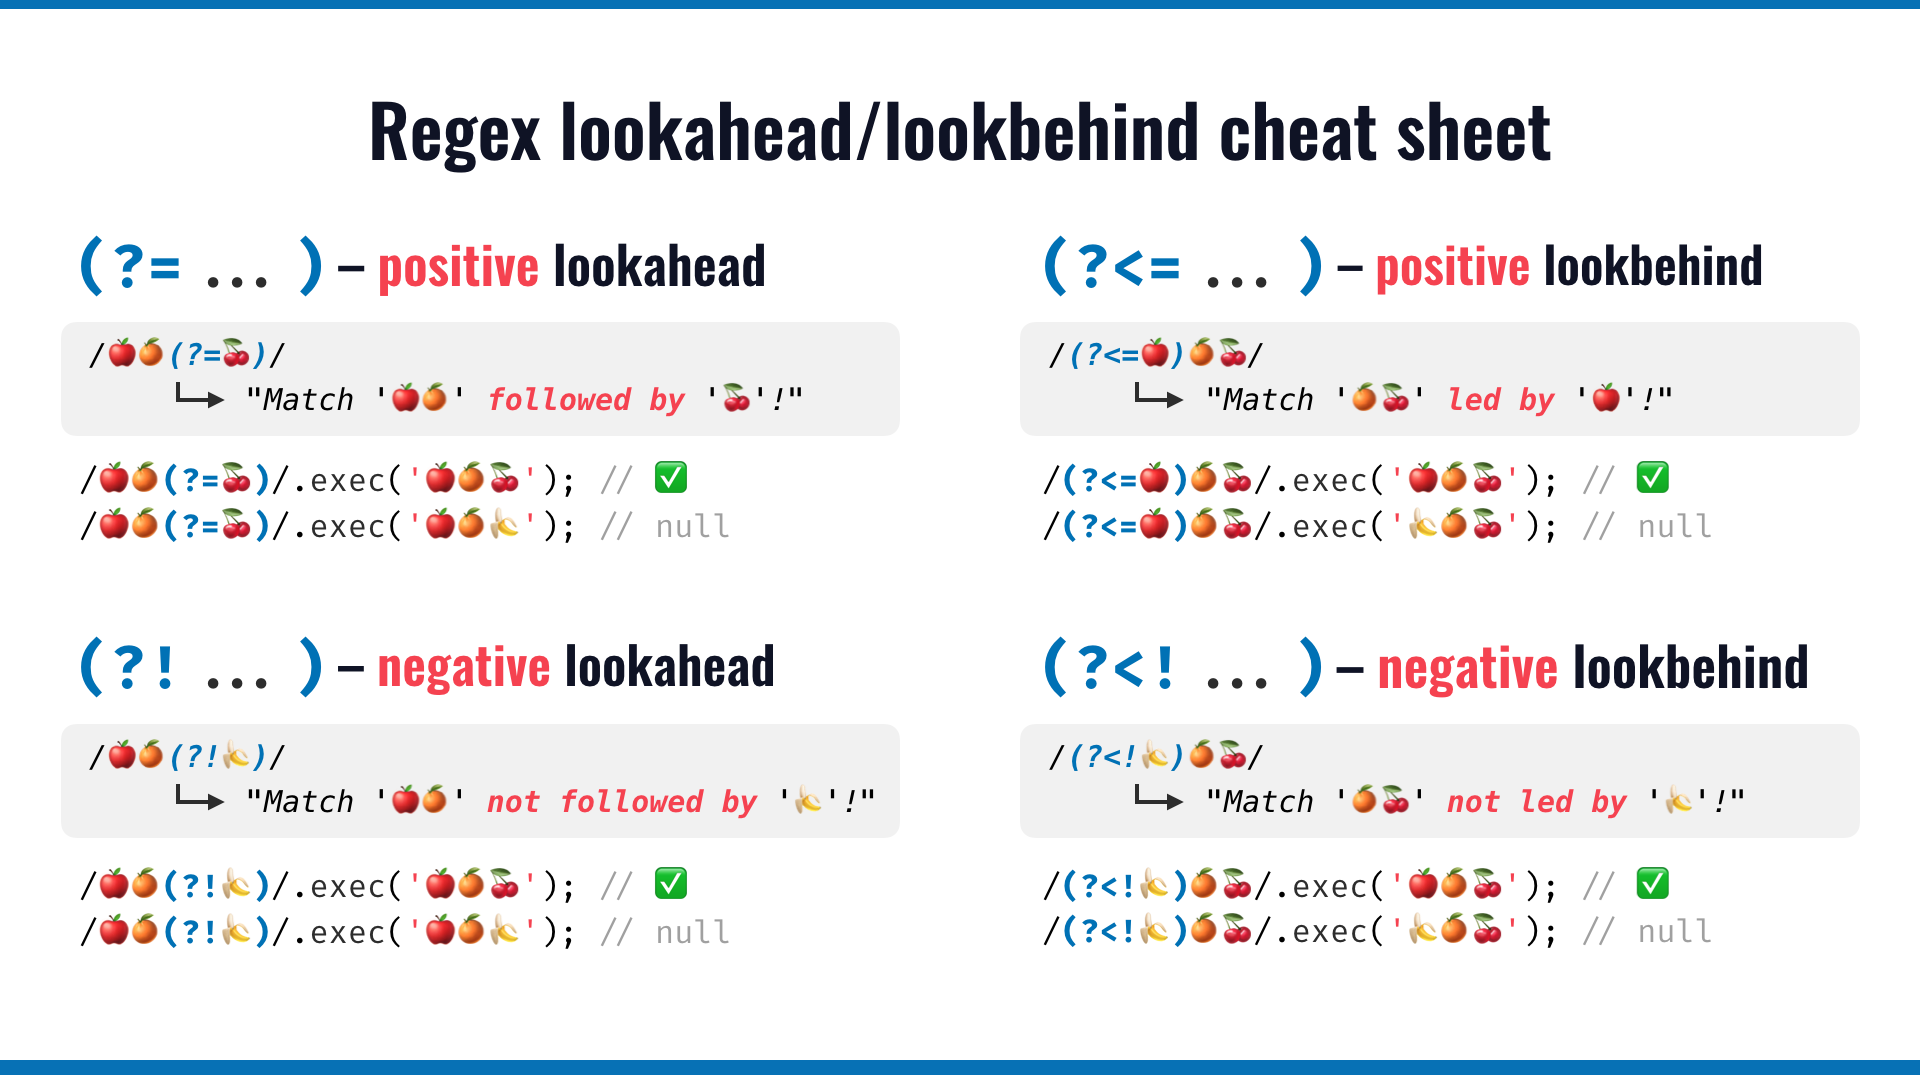
\includegraphics{pcre-look}
  \caption{Positive and Negative Look-ahead and look-behind assertions}
  \labfig{pcre-look}
\end{figure}

\subsection{Comments}

A comment begins with \lstinline|(?#| and ends at the next closing parenthesis.

\subsection{Recursive patterns}

A pattern can refer back to itself recursively or to any subpattern. For example, the pattern \lstinline:\((a*|(?R))*\): will match any combination of balanced parentheses and "a"s.

\newpage
\section{Other Text Processing Tools}

Now that we have discussed the basics of regular expressions, let us see how we can use them in some text processing utilities. We will discuss the following text processing utilities:

\begin{itemize}
  \item \lstinline|tr| - Translate characters.
  \item \lstinline|cut| - Cut out fields (columns) from a line.
  \item \lstinline|grep| - Search for patterns in a file.
  \item \lstinline|sed| - Stream editor - search and replace, insert, select, delete, translate.
  \item \lstinline|awk| - A programming language for text processing.
\end{itemize}

However, these are not all the text processing tools that exist. There are many other text processing utilities that are used in Unix-like systems. Some of them are:

\begin{itemize}
  \item \lstinline|rg| - ripgrep - A search tool that combines the usability of The Silver Searcher (ag) with the raw speed of grep. Useful to find files recursively in a directory or git repository.
  \item \lstinline|fzf| - Fuzzy Finder - A command-line fuzzy finder. Useful to search for files and directories even when you might not know a valid substring of the text. It works by searching for subsequences instead of substrings and other fuzzy search logic. It is extremely powerful when paired with other applications as an interactive select menu.
  \item \lstinline|csvlens| - A tool to view and query CSV files. It is useful to view and query CSV files in a tabular format. It can search for data in a CSV using regex.
  \item \lstinline|pdfgrep| - A tool to search for text in PDF files. It is useful to search for text in PDF files. It can search for text in a PDF using regex. It also supports PCRE2.
\end{itemize}

There are other useful utilities which are not part of GNU coreutils, but are very useful in text processing. Feel free to find such tools, install them, and play around with them. However, we wont be able to discuss those in detail here.

\subsection{tr}

\lstinline|tr| is a command that is used to translate characters. It is used to replace characters in a string with other characters. It is useful when we want to replace a list of characters with another list of characters, or remove a character from a string. It is trivial to create rotation ciphers using \lstinline|tr|.

Without any flags, \lstinline|tr| takes two arguments, \lstinline|LIST1| and \lstinline|LIST2|, which are the two list of characters. \lstinline|LIST1| is the source map and \lstinline|LIST2| is the destination map of the translation. A character can only map to a single character in a translation, however multiple character can map to the same character. That is, it can be many-to-one, but not one-to-many.

\begin{marginfigure}
  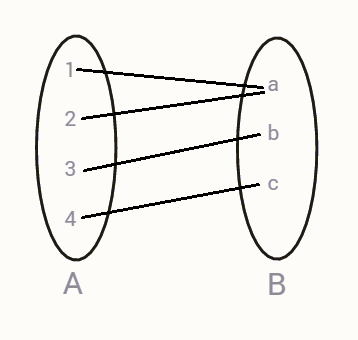
\includegraphics{many-to-one}
  \caption{Many-to-one mapping}
  \labfig{many-to-one}
\end{marginfigure}

A simple example of \lstinline|tr| is to convert a single character to another character.

\begin{lstlisting}
$ echo "hello how are you" | tr 'o' 'e'
helle hew are yeu
\end{lstlisting}

However, the true power of \lstinline|tr| is when we use character lists. We can use character lists to replace multiple characters with other characters.

\begin{lstlisting}
$ echo "hello how are you" | tr 'a-z' 'A-Z'
HELLO HOW ARE YOU
\end{lstlisting}

\lstinline|tr| can also toggle case of characters, that is, the \lstinline|LIST1| and \lstinline|LIST2| can have common characters.

\begin{lstlisting}[language=bash]
$ echo "Hello How Are You" | tr 'a-zA-Z' 'A-Za-z'
hELLO hOW aRE yOU
\end{lstlisting}

We do not need to surround the character ranges in brackets.

\subsubsection{Ciphers}

\begin{definition}[Cipher]
  A cipher is an algorithm for performing encryption or decryption—a series of well-defined steps that can be followed as a procedure. An alternative, less common term is encipherment. To encipher or encode is to convert information into cipher or code. In cryptography, encryption is the process of encoding information. This process converts the original representation of the information, known as plaintext, into an alternative form known as ciphertext. Ideally, only authorized parties can decipher a ciphertext back to plaintext and access the original information.
\end{definition}

One of the common ciphers are rotation ciphers, where each character is replaced by another character that is a fixed number of positions down the alphabet. This is also known as the Caesar cipher, named after Julius Caesar, who is said to have used it to communicate with his generals.

\begin{marginfigure}
  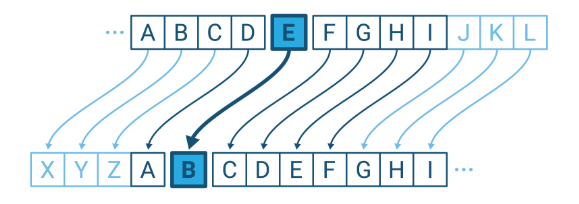
\includegraphics{caesar}
  \caption{Caesar Cipher}
  \labfig{caesar}
\end{marginfigure}

If the shift is 13
\sidenote{
  This is special because the shift of 13 is the same for both encoding and decoding. This is because the English alphabet has 26 characters, and 13 is half of 26. Thus, if we shift by 13, we will get the same character when we shift back by 13.
  It is thus an involution, that is, applying it twice will give the original text.
}
then the cipher is called ROT13. It is a simple letter substitution cipher that replaces a letter with the 13th letter after it in the alphabet. ROT13 is a special case of the Caesar cipher which was developed in ancient Rome.

Let us try to implement ROT13 using \lstinline|tr|.

\begin{lstlisting}[language=bash]
$ echo "hello how are you?" | tr 'a-zA-Z' 'n-za-mN-ZA-M'
uryyb ubj ner lbh?
$ echo "uryyb ubj ner lbh?" | tr 'a-zA-Z' 'n-za-mN-ZA-M'
hello how are you?
\end{lstlisting}

Observe how running the output of the cipher through the same cipher gives us back the original plain-text. This is because ROT13 is an involution cipher.

We can concatenate multiple ranges of characters in the character-lists as seen above, \lstinline|tr| simply converts each character in \lstinline|LIST1| to its corresponding character in \lstinline|LIST2|. The length of both the lists should thus be same. However, if the \lstinline|LIST2| is smaller than \lstinline|LIST1|, \lstinline|tr| will simply repeat the last character of \lstinline|LIST2| as many times as required to make both the lists same length.

\begin{lstlisting}[language=bash]
$ echo "abcdefghijklmnopqrstuvwxyz" | tr 'a-z' '1'
11111111111111111111111111
$ echo "abcdefghijklmnopqrstuvwxyz" | tr 'a-z' '12'
12222222222222222222222222
$ echo "abcdefghijklmnopqrstuvwxyz" | tr 'a-z' '123'
12333333333333333333333333
$ echo "abcdefghijklmnopqrstuvwxyz" | tr 'a-z' '1234-9'
12345678999999999999999999
\end{lstlisting}

The characters in the list are treated as characters, and not digits, thus we cannot replace a character with a multi-digit number. the range \lstinline|1-26| will not result to $26$ numbers from $1$ to $26$, rather, it results in three numbers: $1$, $2$, and $6$. Similarly \lstinline|1-72| means $1,2,3,4,5,6,7,2$.

\begin{lstlisting}[language=bash]
$ echo "abcdefghijklmnopqrstuvwxyz" | tr 'a-z' '1-26'
12666666666666666666666666
$  tr 'a-z' '1-72' <<< "abcdefghijklmnopqrstuvwxyz"
12345672222222222222222222
\end{lstlisting}

We can also repeat a character any arbritrary number of times by using the \lstinline|*| character in the \lstinline|LIST2| inside square brackets.

\begin{lstlisting}[language=bash]
$ echo "abcdefghijklmnopqrstuvwxyz" | tr 'a-z' '1-4[5*10]7'
12345555555555777777777777
\end{lstlisting}

Here the repeat number is actually treated as a number, and thus multi-digit numbers (as shown above) can be used to repeat the character any number of times.

\lstinline|tr| can perform any cipher that does not depend on additional memory or state.

\subsubsection{Deletion}

\lstinline|tr| can also delete or drop characters from a string of characters.
The flag \lstinline|-d| is used to delete characters from the input string.
The syntax is \lstinline|ls -d 'LIST1'|, where \lstinline|LIST1| is the list of characters to delete.

\begin{lstlisting}[language=bash]
$ echo "hi! hello how are you?" | tr -d 'aeiou'
h! hll hw r y?
\end{lstlisting}

Here we are deleting all the vowels from the input string.

We can also use ranges to delete characters.

\begin{lstlisting}[language=bash]
$ echo "hi! hello how are you?" | tr -d 'a-m'
! o ow r you?
\end{lstlisting}

Here we are deleting all the characters from \lstinline|a| to \lstinline|m|.

Sometimes the characters we want to delete is a lot, and its easier to specify the characters we want to keep. We can use the \lstinline|-c| flag to complement the character list, that is, to keep the characters that are in the list.

\begin{lstlisting}[language=bash]
$ echo "hi! hello how are you?" | tr -cd 'a-m'
hihellhae
\end{lstlisting}

Here we are keeping only the characters from \lstinline|a| to \lstinline|m|.
Observe that it also deletes the punctuations, spaces and the newline characters
as well.

This is useful if we want to filter out only some characters from a stream of random characters, for example when trying to generate a random
\sidenote{
  It is not recommended to use \lstinline|/dev/random| instead of \lstinline|/dev/urandom| as it will block if there is a lack of enough entropy. We should totally avoid using \lstinline|RANDOM| variable for cryptographic works since it is not cryptographically secure random number. Computers cannot really generate random numbers, since they are deterministic. Most random number generators simply use external variables like the voltage, temperature, and microphone noise to simulate randomness. This may seem random to humans but is not cryptographically secure for use in generating passwords. There are more secure algorithms to generate passwords. Read more about it
  \href{https://en.wikipedia.org/wiki/Cryptographically\_secure\_pseudorandom\_number\_generator}{here}.
}
password.

\begin{lstlisting}[language=bash]
$ tr -cd 'a-zA-Z0-9' < /dev/urandom | head -c 20 ; echo
8JOzmr4BUbho6wDPaipT
\end{lstlisting}

This uses the \lstinline|/dev/urandom| file to generate random characters, and then filters out only the alphanumeric characters. The \lstinline|head -c 20| is used to print only the first 20 characters, and the \lstinline|echo| is used to print a newline after the password.

\subsubsection{Squeeze}

Finally, \lstinline|tr| can also be used to squeeze characters, that is, to replace multiple consequtive occurrences of a character with a single occurrence. The \lstinline|-s| flag is used to squeeze characters.
It also takes a single argument, which is the list of characters to squeeze.

\marginnote{
  Use single quotes for this example, and not double quotes, as \lstinline|!!| has special meaning in double quotes. It expands to the last run command. This is useful when you write a long command and forget to use \lstinline|sudo|, instead of typing the entire thing again, or using arrow keys, simply type \lstinline|sudo !!| to expand the \lstinline|!!| with the entire previous command.
}
\begin{lstlisting}[language=bash]
$ echo 'Hello!!!!! Using multiple punctuations is not only gramatticaly incorrect but also obnoxious!' | tr -s '!'
Hello! Using multiple punctuations is not only gramatticaly incorrect but also obnoxious!
\end{lstlisting}

\subsection{cut}

If you want to extract a certain column, or a certain range of columns
from a structured text file, doing so using regular expressions can be
a bit cumbersome.

\marginnote{
 Lets try to parse the PCRE regex \lstinline|[^,]*,\\K[^,]*(?=,[^,]*)| to extract the second column from a CSV file. \\ \\
 The first part, \lstinline|[^,]*,| matches the first column, and the \lstinline|\\K| is used to reset the start of the match. This ensures that the first column is present, but not matched and thus not printed.\\ \\
 The second part, \lstinline|[^,]*| matches the second column.
 We are matching as many non-comma characters as possible.\\ \\
 The \lstinline|(?=,[^,]*)| is a lookahead assertion, and is used to match the third column. This ensures that it matches only the second column, and no other column. It will ensure a third column is present, but not match it, thus not printing it. \\ \\
 We had to use \lstinline|\\K| and we could not use a lookbehind assertion, as lookbehind assertions are fixed length, and we do not know the length of the first column. We could have used a lookbehind assertion if we knew the length of the first column.
}
\begin{lstlisting}[language=bash]
$ cat data.csv
name,age,gender
Alice,18,F
Bob,32,M
Carla,23,F
$ grep -P '[^,]*,\K[^,]*(?=,[^,]*)' data.csv -o
age
18
32
23
\end{lstlisting}

As seen above, we can use regular expressions to extract the second column from a CSV file. However, this is not very readable, and can be cumbersome for large files with a lot of columns. This also requires using PCRE to avoid matching the lookbehind and the lookaheads. However, this can be done in an easier manner. This is where the \lstinline|cut| command comes in.

Using \lstinline|cut|, this operation becomes trivial.

\begin{lstlisting}[language=bash]
$ cat data.csv
name,age,gender
Alice,18,F
Bob,32,M
Carla,23,F
$ cut -d, -f2 data.csv
age
18
32
23
\end{lstlisting}

The \lstinline|-d| flag is used to specify the delimiter, and the \lstinline|-f| flag is used to specify the field. The delimiter is the character that separates the fields, and the field is the column that we want to extract. The fields are numbered starting from 1.

\lstinline|cut| can also extract a range of columns.

\marginnote{
  The range is inclusive, that is, it includes the start and end columns.\\ \\
  If the start of the range is absent, it is assumed to be the first column. \\ \\
  If the end of the range is absent, it is assumed to be the last column. \\ \\
  This lets us extract columns even if we do not know the number of columns in the file.
}
\begin{lstlisting}[language=bash]
$ cat data.csv
name,age,gender
Alice,18,F
Bob,32,M
Carla,23,F
$ cut -d, -f1,3 data.csv
name,gender
Alice,F
Bob,M
Carla,F
$ cut -d, -f2-3 data.csv
age,gender
18,F
32,M
23,F
$ cut -d, -f2- data.csv
age,gender
18,F
32,M
23,F
\end{lstlisting}

We can also mention disjoint sets of columns or ranges of columns separated by commas.

\marginnote{
  Here we are using the \lstinline|/etc/passwd| file as an example. The \lstinline|/etc/passwd| file is a text file that contains information about the users on the system. It contains information like the username, user ID, group ID, home directory, and shell. The file is a colon-separated file, where each line contains information about a single user. The fields are separated by colons, and the fields are the username, password (it is not stored, so it is always x), user ID, group ID, user information (this is usually used by modern distrbutions to store the user's full name), home directory, and shell. The file is readable by all users, but only writable by the root user. The file is used by the system to authenticate users and to store information about the users on the system.
}
\begin{lstlisting}[language=bash]
$ cut -d: -f1,5-7 /etc/passwd | tail -n5
dhcpcd:dhcpcd privilege separation:/:/usr/bin/nologin
redis:Redis in-memory data structure store:/var/lib/redis:/usr/bin/nologin
saned:SANE daemon user:/:/usr/bin/nologin
tor::/var/lib/tor:/usr/bin/nologin
test1::/home/test1:/usr/bin/bash
\end{lstlisting}

\begin{exercise}
  Now that you are familiar with the \lstinline|/etc/passwd| file, try to extract the usernames and the home directories of the users. The usernames are the first field, and the home directories are the sixth field. Use the \lstinline|cut| command to extract the usernames and the home directories of the users.
\end{exercise}

\subsubsection{Delimiter}

The default delimiter for \lstinline|cut| is the tab character. However, we can specify the delimiter using the \lstinline|-d| flag. Although it is not required to quote the delimiter, certain characters might be apprehended by the shell and not passed as-is to the command, hence it is always best practice to quote the delimiter using single-quotes. The delimiter has to be a single character, and cannot be more than one character.

The input delimiter can only be speficied if splitting the file by fields, that is, when we are using \lstinline|-f| flag with a field or range of fields.

\subsubsection{Output Delimiter}

The output delimiter by defalut is the same as the input delimiter. However, we can specify the output delimiter using the \lstinline|--output-delimiter| flag. The output delimiter can be a string, and not just a single character. This is useful when we want to change the delimiter of the output file.

\marginnote{
  \lstinline|cut|, like most coreutils, will read the data from standard input (stdin) if no file is specified. This is useful when we want to pipe the output of another command to \lstinline|cut|.
}
\begin{lstlisting}[language=bash]
$ head -n1 /etc/passwd | cut -d: -f5- --output-delimiter=,
root,/root,/usr/bin/bash
$ head -n1 /etc/passwd | cut -d: -f5- --output-delimiter=,,
root,,/root,,/usr/bin/bash
\end{lstlisting}

\subsubsection{Character Range}

The \lstinline|-b| flag is used to extract bytes from a file. The bytes are numbered starting from 1. The byte range is inclusive, that is, it includes the start and end bytes. If the start of the range is absent, it is assumed to be the first byte. If the end of the range is absent, it is assumed to be the last byte.

If we are working with a file with multi-byte characters, the \lstinline|-b| flag will not work as expected, as it will extract bytes, and not characters.
Then we can use the \lstinline|-c| flag to extract characters from a file. The characters are numbered starting from 1. However, in GNU cut, the feature is not yet implemented. If you are using \textbf{freebsd cut} then the difference can be observed.

\begin{lstlisting}[language=bash]
$ head -n1 /etc/passwd | cut -b5-10
:x:0:0
$ head -n1 /etc/passwd | cut -c5-10
:x:0:0
\end{lstlisting}

\subsubsection{Complement}

Sometimes its easier to specify the fields we want to drop, rather than the fields we want to keep. We can use the \lstinline|--complement| flag to drop the fields we specify.

Recall that the second field of the \lstinline|/etc/passwd| file is the password field, which is always \lstinline|x|. We can drop this field using the \lstinline|--complement| flag.

\begin{lstlisting}[language=bash]
$ head -n1 /etc/passwd
root:x:0:0:root:/root:/usr/bin/bash
$ head -n1 /etc/passwd | cut -d: --complement -f2
root:0:0:root:/root:/usr/bin/bash
\end{lstlisting}

\subsubsection{Only Delimited Lines}

Sometimes we have a semi-structured file, where some lines are delimited by a character, and some are not. We can use the \lstinline|--only-delimited| flag to print only the lines that are delimited by the delimiter.

\marginnote{
  Note that if we mention a field number that is not present in the line, \lstinline|cut| will simply print nothing. If we print fields 1 to 3, and there are only 2 fields, it will print only first two fields, etc.
}
\begin{lstlisting}[language=bash]
$ cat data.csv
name,age,gender
Alice,18,F
Bob,32,M
Carla,23,F
# This is a comment
$ cut -d, -f1,3 data.csv
name,gender
Alice,F
Bob,M
Carla,F
# This is a comment
$ cut -d, -f1,3 data.csv  --only-delimited
name,gender
Alice,F
Bob,M
Carla,F
\end{lstlisting}

Cut is a very handy tool for text processing, we will be using it extensively in the upcoming chapters.

\subsection{paste}

\lstinline|paste| is a very simple command that is used to merge lines of files.
It is used to merge lines of files horizontally, that is, to merge lines from multiple files into a single line. It is useful when we want to merge lines from multiple files into a single line, and separate them by a delimiter. It can also be used to join one file into a single line separated by a delimiter.

\begin{lstlisting}[language=bash]
$ cat file1.txt
hello world
this is file1
$ cat file2.txt
this is file2
and it has more lines
than file1
$ paste file1.txt file2.txt
hello world     this is file2
this is file1   and it has more lines
        than file1
\end{lstlisting}

The default delimiter is the tab character, however we can specify the delimiter using the \lstinline|-d| flag.

\begin{lstlisting}[language=bash]
$ paste -d: file1.txt file2.txt
hello world:this is file2
this is file1:and it has more lines
:than file1
\end{lstlisting}

Paste can also be used to merge lines from a single file into a single line.
The \lstinline|-s| flag is used to merge lines from a single file into a single line.
We can specify the delimiter for this as well using the \lstinline|-d| flag.

\begin{lstlisting}[language=bash]
$ paste -d: -s file1.txt
hello world:this is file1
\end{lstlisting}

This is better than using \lstinline|tr '\n' ':'| to replace the newline character with a delimiter, as \lstinline|tr| will also replace the last newline character of the last line, giving a trailing delimiter.

\begin{lstlisting}[language=bash]
$ tr '\n' ':' < file1.txt
hello world:this is file1:
\end{lstlisting}

This is very helpful when we want to find the sum of numbers in a file.

\begin{lstlisting}[language=bash]
$ cat numbers.txt
1
4
2
6
7
2
$ paste -sd+ numbers.txt
1+4+2+6+7+2
$ paste -sd+ numbers.txt | bc
22
\end{lstlisting}

Here we are first using \lstinline|paste| to merge the lines of the file into a single line, separated by the \lstinline|+| character. We then pipe this to \lstinline|bc|, which is a command line calculator, to calculate the sum of the numbers.

\subsection{fold}

Just like we can use \lstinline|paste| to merge lines of a file, we can use \lstinline|fold| to split lines of a file. \lstinline|fold| is a command that is used to wrap lines of a file. It is used to wrap lines of a file to a specified width.

\begin{lstlisting}[language=bash]
$ cat data.txt
123456789
$ fold -w1 data.txt
1
2
3
4
5
6
7
8
9
$ fold -w2 data.txt
12
34
56
78
9
\end{lstlisting}

We can also force \lstinline|fold| to break lines at spaces only, and not in the middle of a word. However, if it is not possible to maintain the maximum width specified if breaking solely on spaces, it will break on non-spaces as well.

\begin{lstlisting}[language=bash]
$ cat text.txt
This is a big block of text
some of these lines can break easily
Whereas_some_are_to_long_to_break
$ fold -sw10 text.txt
This is a
big block
of text
some of
these
lines can
break
easily
Whereas_so
me_are_to_
long_to_br
eak
\end{lstlisting}

This is useful if you want to undo the operation of \lstinline|tr -d '\n'| performed on lines of equal width.

\subsection{grep}

\lstinline|grep| is a command that is used to search for patterns in a file. It is used to search for a pattern in a file, and print the lines that match the pattern.

Grep has a lot of flags and features, and is a very powerful tool for searching for patterns in a file.
It can search using \textbf{BRE}, \textbf{ERE}, and even \textbf{PCRE}.

We will discuss \lstinline|grep| in detail in the next chapter.

\subsection{sed}

\lstinline|sed| is a stream editor that is used to perform basic text transformations on an input stream. It is used to search and replace, insert, select, delete, and translate text.

Sed is a sysadmin's go to tool for perform quick text transformations on files.
It can also perform the changes directly on the file, without needing to write the changes to a new file.

We cover \lstinline|sed| in detail in later chapters.

\subsection{awk}

\lstinline|awk| is a programming language that is used for text processing and data extraction. It is a very powerful tool for text processing, and is used to extract and manipulate data from files.

It has its own programming language, although with very few keywords, and is very easy to learn.

We cover \lstinline|awk| in detail in later chapters.

% \setchapterpreamble[u]{\margintoc}
\chapter{Grep}
\labch{grep}

We have already seen and used \lstinline|grep| throughout this chapter while discussing regex. \lstinline|grep| is a command that is used to search for patterns in a file. It is used to search for a pattern in a file, and print the lines that match the pattern.

The name \lstinline|grep| comes from the \textbf{g/re/p} command in the \textbf{ed} editor. The \textbf{ed} editor is a line editor, and the \textbf{g/re/p} command is used to search for a pattern in a file, and print the lines that match the pattern. The \lstinline|grep| command is a standalone command that is used to search for a pattern in a file, and print the lines that match the pattern.

\lstinline|grep| can use \textbf{BRE} or \textbf{ERE}, or even \textbf{PCRE} if the \lstinline|-P| flag is used. By default, \lstinline|grep| matches using the \textbf{BRE} engine.

\begin{lstlisting}[language=bash]
$ grep "[aeiou]" -o <<< "hello how are you?"
e
o
o
a
e
o
u
\end{lstlisting}

\section{Regex Engine}

However, \lstinline|grep| can also use the \textbf{ERE} engine using the \lstinline|-E| flag. This is useful when we want to use the special characters like \lstinline|+|, \lstinline|?|, \lstinline|(|, \lstinline|)|, \lstinline|{|, \lstinline|}|, and \lstinline:|: without escaping them.
\sidenote{
 There is also an executable called \lstinline|egrep|, which is the same as \lstinline|grep -E|. It is provided for compatibility with older Unix systems. It is not recommended to use \lstinline|egrep|, as it is deprecated and not present in all systems. You should use \lstinline|grep -E| instead.
}

\begin{lstlisting}[language=bash]
$ grep -E "p+" -o <<< "apple and pineapples"
pp
p
pp
\end{lstlisting}

Sometimes, it is required to not use regex at all, and simply search for a string. We can use the \lstinline|-F| flag to search for a fixed string, and not a regex.
This will search for any line that has the substring. Any symbol that has special meaning in regex will be treated as a literal character.

\begin{lstlisting}[language=bash]
$ grep -F "a+b*c=?" -o <<< "What is a+b*c=?"
a+b*c=?
\end{lstlisting}

This mode is useful if you want to match any arbritary string in a file, and do not know what the string is going to be, thus not allowing you to escape the special characters.

\begin{lstlisting}[language=bash]
$ cat data.txt
Hello, this is a file
with a lot of equations
1. a^2 + b^2 = c^2 for right angle triangles
2. E = mc^2
3. F = ma
4. The meaning of life, the universe, and everything = 42
$ read -r -p "What to search for? " pattern
What to search for? ^2
$ grep "$pattern" data.txt
2. E = mc^2
$ grep -F "$pattern" data.txt
1. a^2 + b^2 = c^2 for right angle triangles
2. E = mc^2
\end{lstlisting}

In the above example, you can see a file full of equations, thus special symbols.
If we want to dynamically input what to search for, we can use the \lstinline|read| command to read the input from the user, and then use \lstinline|grep| to search for the pattern. If we use the \lstinline|-F| flag, we can search for the pattern as a fixed string, and not as a regex.

Here we wanted to find all the quadratic equations, and thus searched for \lstinline|^2|.
However, observe that the \lstinline|grep|, without the \lstinline|-F| flag, did not match the first equation which has multiple \lstinline|^2| in it, because it is treating \lstinline|^| with its special meaning of \textbf{start of line anchor}.

If we were statically providing the search string, we can simply escape the special characters, and use \lstinline|grep| without the \lstinline|-F| flag. But in cases like this, it is easier to simply use the \lstinline|-F| to not use regular expression and simply find substrings.

\section{PCRE}

Similarly, there are situations where the ERE engine is not powerful enough and we need to use the \textbf{PCRE} engine. We can use the \lstinline|-P| flag to use the PCRE engine.

\begin{lstlisting}[language=bash]
$ cat data.txt
Hello, this is a file
with a lot of equations
1. a^2 + b^2 = c^2 for right angle triangles
2. E = mc^2
3. F = ma
4. The meaning of life, the universe, and everything = 42
$ grep -P "c\^2" data.txt
1. a^2 + b^2 = c^2 for right angle triangles
2. E = mc^2
$ grep -P "c\^2(?=.*triangle)" data.txt
1. a^2 + b^2 = c^2 for right angle triangles
\end{lstlisting}

Here, if we want to find all the equations with \lstinline|c^2|, but only if that equation also mentions "triangle" somewhere after the \lstinline|c^2|, then we can use lookahead assertions of PCRE to accomplish that.
Here, the \lstinline|.*| matches any character zero or more times, and the \lstinline|triangle| matches the string "triangle".
Putting it inside a lookahead assertion (\lstinline|(?= )|) ensures that the pattern is present, but not part of the match.

This can be confirmed by using the \lstinline|-o| flag to print only the matched part of the line.

\begin{lstlisting}[language=bash]
$ grep -P "c\^2(?=.*triangle)" -o data.txt
c^2
\end{lstlisting}

\section{Print Only Matching Part}

We have been using the \lstinline|-o| flag extensively to print only the matching part of the line. This is useful when we want to extract only the part of the line that matches the pattern and not the entire line.
This is also very useful for debugging regex, as we can see what part of the line is actually matching the pattern.

If we do not use \lstinline|-o|, then any line having one or more match will be printed entirely, and the matches will be colored red
\sidenote{
  \lstinline|grep| will color the match only if you pass the flag \lstinline|--color=always|, or if the flag is set to \lstinline|--color=auto| and the terminal supports color output. Otherwise no ANSI-escape code is printed by grep.\\ \\
  You can also change the color of the match by setting the \lstinline|GREP_COLORS| environment variable. The default color is red, but you can change it to any color you want.
}
,however, if two consequtive matches are present, it becomes hard to distinguish between the two matches.

If we use the \lstinline|-o| flag, then only the matching part of the line is printed, and each match is printed on a new line, making it easy to see exactly which parts are matched.

\begin{lstlisting}[language=bash]
$ grep -E "o{,3}" <<< "hellooooo"
hellooooo
$ grep -Eo "o{,3}" <<< "hellooooo"
ooo
oo
\end{lstlisting}

In the above example, we ask \lstinline|grep| to match the pattern \lstinline|o{,3}|, that is, match the letter \lstinline|o| zero to three times. If we do not use the \lstinline|-o| flag, then the entire line is printed, and the matches are colored red. This however creates a confusion, even though all the $5$ $o$'s are matched, they cannot obviously be a single match, since a single match can only be of a maximum of $3$ $o$'s. So how are the matches grouped? Is it $3$ $o$'s followed by $1$ $o$ followed by another $o$? Is it $2$ $o$'s followed by $2$ $o$'s followed by one $o$? There seems to be no way to tell from the first output.

However, if we use the \lstinline|-o| flag, then only the matching part of the line is printed, and each match is printed on a new line. It then becomes clear that grep will greedily match as much as possible first, so the first three $o$'s are matched, and then the remaining are grouped as a single match.

\section{Matching Multiple Patterns}

\subsection{Disjunction}

If we want to match multiple patterns, we can use the \lstinline|-e| flag to specify multiple patterns. This is useful when we want to match multiple patterns, and not just a single pattern. Any line containing one or more of the patterns we are searching for will be printed. This is like using an \textbf{OR} clause.

\marginnote{
  In this example, we want to find lines that match the word "file" or the word "life". We can use the \lstinline|-e| flag to specify multiple patterns. The \lstinline|-e| flag is automatically implied if we are searching for a single pattern, however, if we are searching for more than one pattern, we have specify it for all of the patterns, including the first one.
}
\begin{lstlisting}[language=bash]
$ cat data.txt
Hello, this is a file
with a lot of equations
1. a^2 + b^2 = c^2 for right angle triangles
2. E = mc^2
3. F = ma
4. The meaning of life, the universe, and everything = 42
$ grep "file" data.txt
Hello, this is a file
$ grep -e "file" -e "life" data.txt
Hello, this is a file
4. The meaning of life, the universe, and everything = 42
\end{lstlisting}

\subsection{Conjunction}

If we want to match lines that contain all of the patterns we are searching for, we can pipe the output of one \lstinline|grep| to another, to do iterative filtering.

If we want to find lines which start with a number, and also contain the word "a", then we can use two greps to accomplish this.

\marginnote{
  In this example, first we show each of the pattern we are matching, and that they output multiple lines. Then finally we combine both the patterns using pipe to find only the common line in both the outputs. The patterns can be specified in either order. We need to provide the file only in the first grep, and we should \textbf{not} provide a file name to any of the other greps, otherwise it will not use the output of the previous grep as input and just filter from the file instead. \\ \\
  Here the regex \lstinline|^[0-9]| matches any line that starts with a number.
  And the regex \lstinline|\\ba\\b| matches any line that contains the word "a".
  The \lstinline|\\b| is a word boundary, and matches the start or end of a word. Thus it will match the word "a" and not the letter "a" in a word.
}
\begin{lstlisting}[language=bash]
$ cat data.txt
Hello, this is a file
with a lot of equations
1. a^2 + b^2 = c^2 for right angle triangles
2. E = mc^2
3. F = ma
4. The meaning of life, the universe, and everything = 42
$ grep '\ba\b' data.txt
Hello, this is a file
with a lot of equations
1. a^2 + b^2 = c^2 for right angle triangles
$ grep '^[0-9]' data.txt
1. a^2 + b^2 = c^2 for right angle triangles
2. E = mc^2
3. F = ma
4. The meaning of life, the universe, and everything = 42
$ grep '\ba\b' data.txt  | grep '[0-9]'
1. a^2 + b^2 = c^2 for right angle triangles
\end{lstlisting}

\section{Read Patterns from File}

If we have a lot of patterns to search for, we can put them in a file, and use the \lstinline|-f| flag to read the patterns from the file. Each line of the file
is treated as a separate pattern, and any line that matches any of the patterns will be printed.
The type of regex engine used depends on whether \lstinline|-E|, \lstinline|-P|, or \lstinline|-F| is used.

\begin{lstlisting}[language=bash]
$ cat data.txt
p+q=r
apple
e*f=g
$ cat pattern
p+
e*
$ grep -G -f pattern data.txt  -o
p+
e
e
$ grep -F -f pattern data.txt  -o
p+
e*
$ grep -E -f pattern data.txt  -o
p
pp
e
e
\end{lstlisting}

\section{Ignore Case}

If we want to ignore the case of the pattern, we can use the \lstinline|-i| flag. This is useful when we want to match a pattern, but do not care about the case of the pattern, or we are not sure what the case is.

\begin{lstlisting}[language=bash]
$ grep 'apple' /usr/share/dict/words | head
appleberry
appleblossom
applecart
apple-cheeked
appled
appledrane
appledrone
apple-eating
apple-faced
apple-fallow
$ grep -i 'apple' /usr/share/dict/words | head
Apple
appleberry
Appleby
appleblossom
applecart
apple-cheeked
appled
Appledorf
appledrane
appledrone
\end{lstlisting}

As seen above, the first \lstinline|grep| matches only the lines that contain the word "apple", and not "Apple". However, the second \lstinline|grep| matches both "apple" and "Apple".

\section{Invert Match}

Sometimes its easier to specify the patterns we do not want to match, rather than the patterns we want to match. We can use the \lstinline|-v| flag to invert the match, that is, to print only the lines that do not match the pattern.

\begin{lstlisting}[language=bash]
$ cat data.txt
apple
banana
blueberry
blackberry
raspberry
strawberry
$ grep -v 'berry' data.txt
apple
banana
\end{lstlisting}

This is useful when we want to filter out some arbritary stream of data for some patterns.

\marginnote{
  In this example, we are filtering out all the users that have the shell set to \lstinline|nologin|. These are users which cannot be logged into. We can use the \lstinline|-v| flag to invert the match, and print only the users that do not have the shell set to \lstinline|nologin|. Effectively printing all the accounts in the current system that can be logged into.
  \textbf{ntp} uses the \lstinline|/bin/false| shell, which is used to prevent the user from logging in, but is not the same as \lstinline|/usr/bin/nologin|, which is used to prevent the user from logging in and also prints a message to the user.
}
\begin{lstlisting}[language=bash]
$ grep -v 'nologin$' /etc/passwd
root:x:0:0:root:/root:/usr/bin/bash
git:x:971:971:git daemon user:/:/usr/bin/git-shell
ntp:x:87:87:Network Time Protocol:/var/lib/ntp:/bin/false
sayan:x:1000:1001:Sayan:/home/sayan:/bin/bash
test1:x:1001:1002::/home/test1:/usr/bin/bash
\end{lstlisting}

\section{Anchoring}

If we want to match a pattern only at the start of the line, or at the end of the line, we can use the \lstinline|^| and \lstinline|$| anchors respectively.

However, in \lstinline|grep|, if we want to match a pattern that is the entire line, we can use the \lstinline|-x| flag. This is useful when we want to match the entire line, and not just a part of the line.
This is same as wrapping the entire pattern in \lstinline|^$|, but is more readable.

Similarly, if we want to match a pattern that is a word, we can use the \lstinline|-w| flag. This is useful when we want to match a word, and not a part of a word.
This is same as wrapping the entire pattern in \lstinline|\\b|, but is more readable.

\marginnote{
  Observe in this example, if we do not use the \lstinline|-w| flag
  then words that have the substring "apple" will also be matched.
  However, when we use the \lstinline|-w| flag, only the word "apple"
  is matched as a whole word.
}
\begin{lstlisting}[language=bash]
$ grep 'apple' /usr/share/dict/words | tail
stapple
star-apple
strapple
thorn-apple
thrapple
toffee-apple
undappled
ungrapple
ungrappled
ungrappler
$ grep -w 'apple' /usr/share/dict/words | tail
may-apple
oak-apple
pine-apple
pond-apple
rose-apple
snap-apple
sorb-apple
star-apple
thorn-apple
toffee-apple
\end{lstlisting}

\section{Counting Matches}

Sometimes all we want is to see how many lines match the pattern, and not the lines themselves. We can use the \lstinline|-c| flag to count the number of lines that match the pattern.
This is exactly same as piping the output of \lstinline|grep| to \lstinline|wc -l|, but is more readable.

\begin{lstlisting}[language=bash]
$ grep -c 'apple' /usr/share/dict/words
101
$ grep -ic 'apple' /usr/share/dict/words
107
\end{lstlisting}

From this we can quickly see that there are $107-101=6$ lines that
contain the word "Apple" in the file.

We can also print those lines using the \lstinline|diff| command.

\begin{lstlisting}[language=bash]
$ diff <(grep apple /usr/share/dict/words) <(grep -i apple /usr/share/dict/words)
0a1
> Apple
1a3
> Appleby
5a8
> Appledorf
10a14
> Applegate
28a33
> Appleseed
31a37
> Appleton
\end{lstlisting}

Or by using the \lstinline|comm| command.

\begin{marginfigure}
  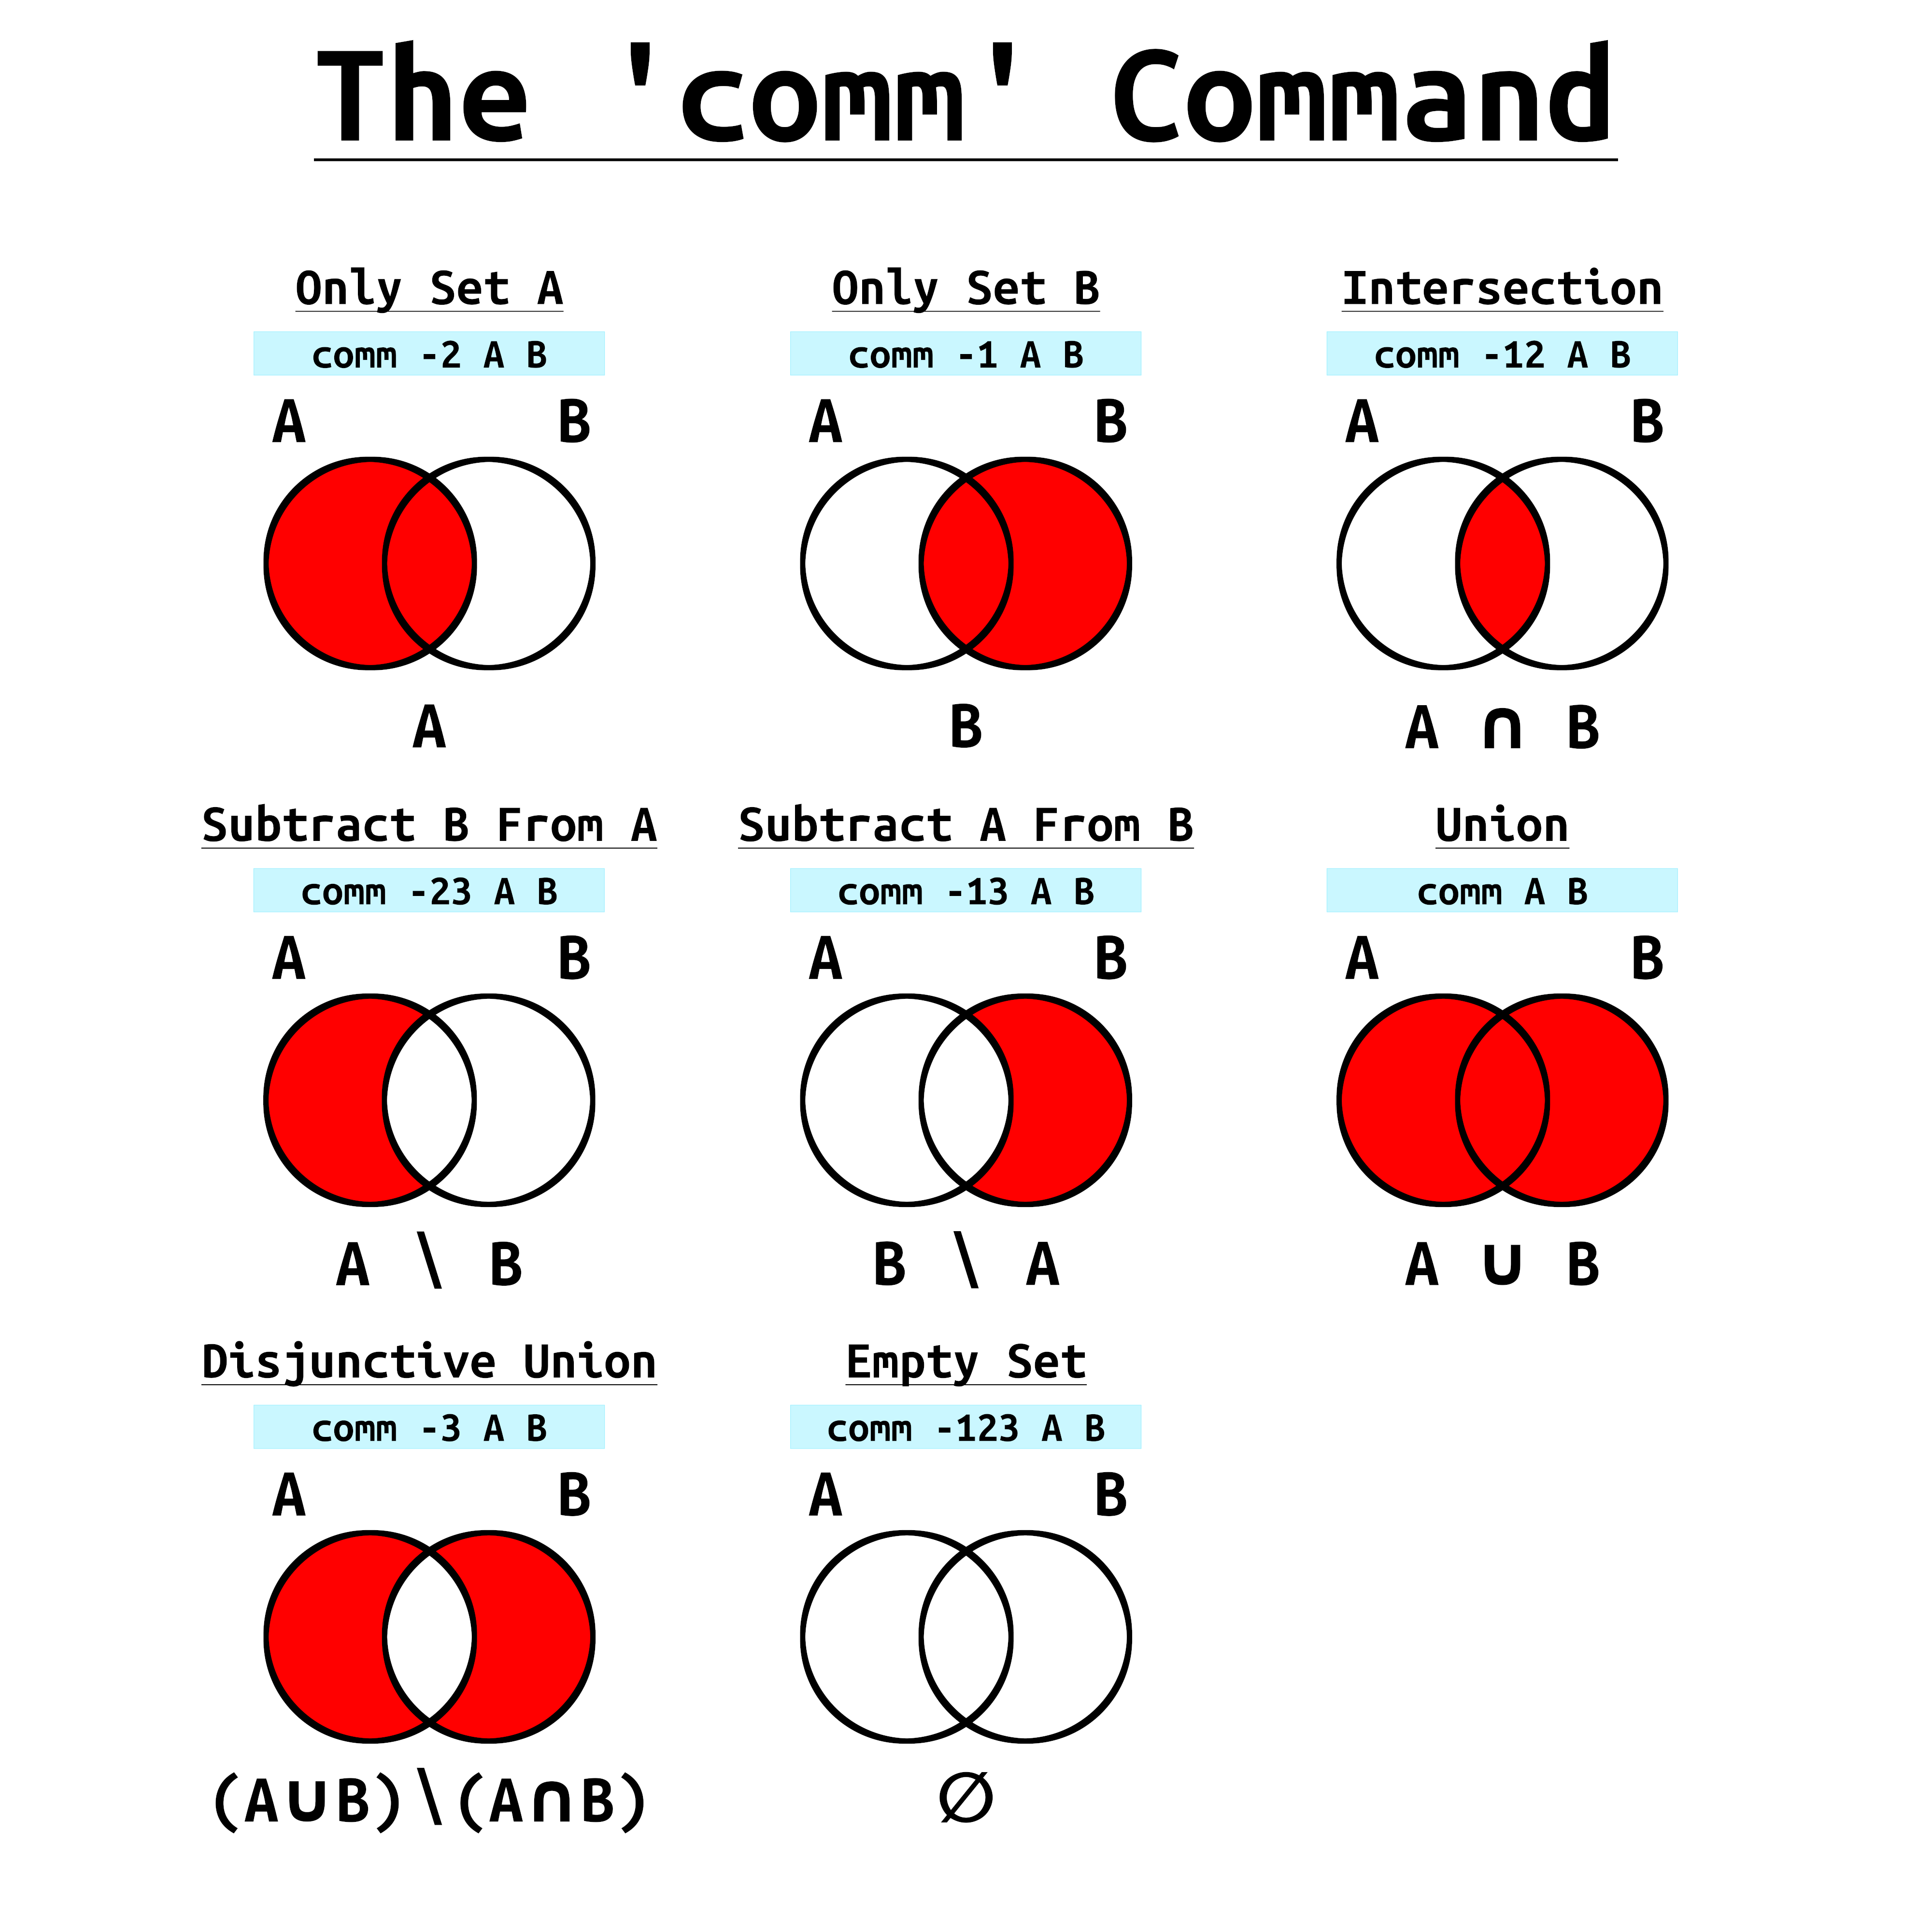
\includegraphics{comm.png}
  \caption{The \lstinline|comm| command}
  \labfig{comm}
\end{marginfigure}

The \lstinline|comm| command is used to compare two sorted files line by line. It is used to find lines that are common, or different between two files. The \lstinline|comm| command requires the input files to be \textbf{sorted}, and it will not work if the files are not sorted. The \lstinline|comm| command has three numbered columns, the first column is the lines that are unique to the first file, the second column is the lines that are unique to the second file, and the third column is the lines that are common to both files. The \lstinline|comm| command is useful when we want to compare two files, and find the differences between them, or find the lines common between them.
\marginnote{
  Observe that we had to sort the files before using \lstinline|comm|, as \lstinline|comm| requires the files to be sorted. We can use the \lstinline|<(command)| syntax to pass the output of a command as a file to another command. This is called process substitution.
}
\begin{lstlisting}[language=bash]
$ comm -13 <(grep apple /usr/share/dict/words | sort) <(grep -i apple /usr/share/dict/words | sort)
Apple
Appleby
Appledorf
Applegate
Appleseed
Appleton
\end{lstlisting}

\section{Print Filename}

Sometimes, we may want to search for a pattern in multiple files, and we want to know which file contains the pattern. We can use the \lstinline|-H| flag to print the filename along with the matched line. This is however the default behaviour in GNU grep if multiple files are passed.

\marginnote{
  In this example, we are passing all the \lstinline|.txt| files in the current directory to \lstinline|grep|, and searching for patterns. The \lstinline|-H| flag is implicit and is used to print the filename along with the matched line. This is useful when we are searching for a pattern in multiple files, and we want to know which file contains the pattern.
}
\begin{lstlisting}[language=bash]
$ cat hello.txt
hello world
hello universe
$ cat linux.txt
this is linux
$ grep hello *txt
hello.txt:hello world
hello.txt:hello universe
$ grep this *txt
linux.txt:this is linux
$ grep i *txt
hello.txt:hello universe
linux.txt:this is linux
\end{lstlisting}

But if we want to suppress the printing of the filename, we can use the \lstinline|-h| flag. This is useful when we are searching for a pattern in multiple files, and we do not want to know which file contains the pattern, just the line.

\begin{lstlisting}[language=bash]
$ cat hello.txt
hello world
hello universe
$ cat linux.txt
this is linux
$ grep -h hello *txt
hello world
hello universe
$ grep -h this *txt
this is linux
$ grep -h i *txt
hello universe
this is linux
\end{lstlisting}

Similarly, if we want to print the filename only if there are multiple files, we can use the \lstinline|-l| flag. This will print \textbf{only} the name of the file that has one or more matches. This mode does not print the filename multiple time even if it has multiple matches on same or different lines.
Thus this is not same as \lstinline/grep pattern files... | cut -d: -f1/.
Rather it is same as \lstinline/grep pattern files... | cut -d: -f1 | uniq/

\section{Limiting Output}

Although we can use \lstinline|head| and \lstinline|tail| to limit the number of lines of output of \lstinline|grep|, \lstinline|grep| also has the \lstinline|-m| flag to limit the number of matches. This is useful when we want to see only the first few matches, and not all the matches.

\marginnote{
  The benefit of using \lstinline|-m| instead of \lstinline|head| is that the output will remain colored if coloring is supported, although it is not visible here, try running both to observe the difference.
}
\begin{lstlisting}[language=bash]
$ grep 'nologin' /etc/passwd
bin:x:1:1::/:/usr/bin/nologin
daemon:x:2:2::/:/usr/bin/nologin
mail:x:8:12::/var/spool/mail:/usr/bin/nologin
ftp:x:14:11::/srv/ftp:/usr/bin/nologin
http:x:33:33::/srv/http:/usr/bin/nologin
nobody:x:65534:65534:Kernel Overflow User:/:/usr/bin/nologin
dbus:x:81:81:System Message Bus:/:/usr/bin/nologin
systemd-coredump:x:984:984:systemd Core Dumper:/:/usr/bin/nologin
systemd-network:x:982:982:systemd Network Management:/:/usr/bin/nologin
systemd-oom:x:981:981:systemd Userspace OOM Killer:/:/usr/bin/nologin
systemd-journal-remote:x:980:980:systemd Journal Remote:/:/usr/bin/nologin
systemd-journal-upload:x:979:979:systemd Journal Upload:/:/usr/bin/nologin
systemd-resolve:x:978:978:systemd Resolver:/:/usr/bin/nologin
systemd-timesync:x:977:977:systemd Time Synchronization:/:/usr/bin/nologin
tss:x:976:976:tss user for tpm2:/:/usr/bin/nologin
uuidd:x:68:68::/:/usr/bin/nologin
avahi:x:974:974:Avahi mDNS/DNS-SD daemon:/:/usr/bin/nologin
named:x:40:40:BIND DNS Server:/:/usr/bin/nologin
dnsmasq:x:973:973:dnsmasq daemon:/:/usr/bin/nologin
geoclue:x:972:972:Geoinformation service:/var/lib/geoclue:/usr/bin/nologin
_talkd:x:970:970:User for legacy talkd server:/:/usr/bin/nologin
nbd:x:969:969:Network Block Device:/var/empty:/usr/bin/nologin
nm-openconnect:x:968:968:NetworkManager OpenConnect:/:/usr/bin/nologin
nm-openvpn:x:967:967:NetworkManager OpenVPN:/:/usr/bin/nologin
nvidia-persistenced:x:143:143:NVIDIA Persistence Daemon:/:/usr/bin/nologin
openvpn:x:965:965:OpenVPN:/:/usr/bin/nologin
partimag:x:110:110:Partimage user:/:/usr/bin/nologin
polkitd:x:102:102:PolicyKit daemon:/:/usr/bin/nologin
rpc:x:32:32:Rpcbind Daemon:/var/lib/rpcbind:/usr/bin/nologin
rpcuser:x:34:34:RPC Service User:/var/lib/nfs:/usr/bin/nologin
rtkit:x:133:133:RealtimeKit:/proc:/usr/bin/nologin
sddm:x:964:964:SDDM Greeter Account:/var/lib/sddm:/usr/bin/nologin
usbmux:x:140:140:usbmux user:/:/usr/bin/nologin
qemu:x:962:962:QEMU user:/:/usr/bin/nologin
cups:x:209:209:cups helper user:/:/usr/bin/nologin
dhcpcd:x:959:959:dhcpcd privilege separation:/:/usr/bin/nologin
redis:x:958:958:Redis in-memory data structure store:/var/lib/redis:/usr/bin/nologin
saned:x:957:957:SANE daemon user:/:/usr/bin/nologin
tor:x:43:43::/var/lib/tor:/usr/bin/nologin
$ grep 'nologin' /etc/passwd | head -n5
bin:x:1:1::/:/usr/bin/nologin
daemon:x:2:2::/:/usr/bin/nologin
mail:x:8:12::/var/spool/mail:/usr/bin/nologin
ftp:x:14:11::/srv/ftp:/usr/bin/nologin
http:x:33:33::/srv/http:/usr/bin/nologin
$ grep 'nologin' /etc/passwd -m5
bin:x:1:1::/:/usr/bin/nologin
daemon:x:2:2::/:/usr/bin/nologin
mail:x:8:12::/var/spool/mail:/usr/bin/nologin
ftp:x:14:11::/srv/ftp:/usr/bin/nologin
http:x:33:33::/srv/http:/usr/bin/nologin
\end{lstlisting}

\begin{lstlisting}[language=bash]
$ cat hello.txt
hello world
hello universe
$ cat linux.txt
this is linux
$ grep -l hello *txt
hello.txt
$ grep -l this *txt
linux.txt
$ grep -l i *txt
hello.txt
linux.txt
\end{lstlisting}

\section{Quiet Quitting}

No, we are not talking about the recent trend of doing the bare minimum in a job.

If we want to suppress the output of \lstinline|grep|, and only see if the pattern was found or not, we can use the \lstinline|-q| flag. This is useful when we want to use \lstinline|grep| in a script, and we do not want to see the output of \lstinline|grep|, just the exit status.
This also implies \lstinline|-m1|, as we can determine the exit status of \lstinline|grep| as soon as we find the first match.

\marginnote{
  In this example we use concepts such as \lstinline|if| and \lstinline|then| to check the exit status of \lstinline|grep|. If the exit status is $0$, then the pattern was found, and we print "world mentioned". If the exit status is $1$, then the pattern was not found, and we do not print anything. \\
  \lstinline|$?| is a special variable that stores the exit status of the last command. If the exit status is $0$, then the command was successful, and if the exit status is $1$, then the command failed. \\
  We will cover these in later chapters.
}
\begin{lstlisting}[language=bash]
$ cat hello.txt
hello world
hello universe
$ grep -q 'world' hello.txt
$ echo $?
0
$ if grep -q 'world' hello.txt ; then echo "world mentioned" ; fi
world mentioned
$ if grep -q 'galaxy' hello.txt ; then echo "galaxy mentioned" ; fi
\end{lstlisting}

\section{Numbering Lines}

If we want to number the lines that match the pattern, we can use the \lstinline|-n| flag. This is useful when we want to see the line number of the lines that match the pattern.

\begin{lstlisting}[language=bash]
$ cat hello.txt
hello world
hello universe
$ grep -n 'hello' hello.txt
1:hello world
2:hello universe
\end{lstlisting}

\section{Recursive Search}

\lstinline|grep| can also search for patterns in directories and subdirectories recursively. We can use the \lstinline|-r| flag to achieve this. This is useful when we want to search for a pattern in multiple files, and we do not know which files contain the pattern, or if the files are nested deeply inside directories.

By default it starts searching from the current directory, but we can specify the directory to start searching from as the second argument.

\begin{lstlisting}[language=bash]
$ mkdir -p path/to/some/deeply/nested/folders/like/this
mkdir: created directory 'path'
mkdir: created directory 'path/to'
mkdir: created directory 'path/to/some'
mkdir: created directory 'path/to/some/deeply'
mkdir: created directory 'path/to/some/deeply/nested'
mkdir: created directory 'path/to/some/deeply/nested/folders'
mkdir: created directory 'path/to/some/deeply/nested/folders/like'
mkdir: created directory 'path/to/some/deeply/nested/folders/like/this'
$ echo hello > path/to/some/deeply/nested/folders/like/this/hello.txt
$ echo "hello world" > path/world.txt
$ grep -r hello
path/world.txt:hello world
path/to/some/deeply/nested/folders/like/this/hello.txt:hello
$ grep -r hello path/to/
path/to/some/deeply/nested/folders/like/this/hello.txt:hello
\end{lstlisting}

\section{Context Line Control}

Sometimes it is useful to see a few lines before or after the actual line that
contains the matched pattern. We can use the \lstinline|-A|, \lstinline|-B|, and \lstinline|-C| flags to control the number of lines to print after, before, and around the matched line respectively.
\sidenote{
  The \lstinline|-A| flag is for printing lines \textbf{after} the match, the \lstinline|-B| flag is for printing lines \textbf{before} the match, and the \lstinline|-C| flag is for printing lines both \textbf{before} and \textbf{after} the match.
}

\begin{lstlisting}[language=bash]
$ grep -n sayan /etc/passwd
37:sayan:x:1000:1001:Sayan:/home/sayan:/bin/bash
$ grep -n sayan /etc/passwd -A2
37:sayan:x:1000:1001:Sayan:/home/sayan:/bin/bash
38-qemu:x:962:962:QEMU user:/:/usr/bin/nologin
39-cups:x:209:209:cups helper user:/:/usr/bin/nologin
$ grep -n sayan /etc/passwd -B2
35-sddm:x:964:964:SDDM Greeter Account:/var/lib/sddm:/usr/bin/nologin
36-usbmux:x:140:140:usbmux user:/:/usr/bin/nologin
37:sayan:x:1000:1001:Sayan:/home/sayan:/bin/bash
$ grep -n sayan /etc/passwd -C2
35-sddm:x:964:964:SDDM Greeter Account:/var/lib/sddm:/usr/bin/nologin
36-usbmux:x:140:140:usbmux user:/:/usr/bin/nologin
37:sayan:x:1000:1001:Sayan:/home/sayan:/bin/bash
38-qemu:x:962:962:QEMU user:/:/usr/bin/nologin
39-cups:x:209:209:cups helper user:/:/usr/bin/nologin
\end{lstlisting}

These were some of the flags that can be used with \lstinline|grep| to control the output. There are many more flags that can be used with \lstinline|grep|, and you can see them by running \lstinline|man grep|.

Now that we have learnt some of the flags on their own, let us try to accomplish certain tasks using multiple flags together.

\section{Finding Lines Common in Two Files}

If we have two files which has some lines of text, and our job is to find
the lines that are common in both, we can use \lstinline|comm| if the files
are sorted, or we can sort the files before passing it to \lstinline|comm| if we are allowed to have the output sorted.

But if we are not allowed to sort the files, we can use \lstinline|grep| to accomplish this.

\begin{lstlisting}[language=bash]
$ cat file1.txt
this is file1
this.*
a common line
is to check if it misinteprets regex
apple
$ cat file2.txt
this is file2
this.*
a common line
is to check if we are checking fixed strings
pineapple
\end{lstlisting}

Ideally the lines that should be detected as being common are the lines

\begin{lstlisting}
this.*
a common line
\end{lstlisting}

Remember that grep allows using a file as the pattern, and it will match any line that matches any of the patterns in the file.
Let us try to use it to provide one file as a pattern, and the other file as the input.

\begin{lstlisting}[language=bash]
$ grep -f file2.txt file1.txt
this is file1
this.*
a common line
\end{lstlisting}

Observe that it is also matching the line \lstinline|this is file1|, which is not common in both the files. This is because the \lstinline|.*| in the pattern \lstinline|this.*| is being interpreted as a regex, and not as a literal character. We can use the \lstinline|-F| flag to treat the pattern as a fixed string, and not as a regex.

\begin{lstlisting}[language=bash]
$ grep -Ff file2.txt file1.txt
this.*
a common line
\end{lstlisting}

So is that it? It looks like we are getting the correct output.
Not yet. If we reverse the order of files, we see that we are not getting the correct output.

\begin{lstlisting}[language=bash]
$ grep -Ff file1.txt file2.txt
this.*
a common line
pineapple
\end{lstlisting}

This is because the \lstinline|apple| in \lstinline|file1.txt| is matching the word \lstinline|pineapple| in \lstinline|file2.txt| as a substring.

If we want to print only lines that match the entire line, we can use the \lstinline|-x| flag.

\begin{lstlisting}[language=bash]
$  grep -Fxf file1.txt file2.txt
this.*
a common line
\end{lstlisting}

Now we are getting the correct output, in the original file order.

If we were to use \lstinline|comm|, we would have to sort the files first, and then use \lstinline|comm| to find the common lines.

\begin{lstlisting}[language=bash]
$ comm -12 file1.txt  file2.txt
comm: file 1 is not in sorted order
comm: file 2 is not in sorted order
comm: input is not in sorted order
$ comm -12 <( sort file1.txt)  <(sort file2.txt)
a common line
this.*
\end{lstlisting}

Observe how the order of output is different.

The trick to mastering grep is to understand the flags, and how they can be combined to accomplish the task at hand. The more you practice, the more you will understand how to use grep effectively. Refer to the practice questions in the VM.


% \setchapterpreamble[u]{\margintoc}
\chapter{Shell Variables}
\labch{variables}

We have seen how to execute commands in the linux shell, and also how to
combine those commands to perform complex tasks. However, to make really
powerful scripts, we need to store the output of commands, and also store
intermediate results. This is where variables come in. In this chapter,
we will learn how to create, manipulate, and use variables in the shell.

\section{Creating Variables}

There are two types of variables in the shell: \textbf{Environment Variables}
and \textbf{Shell Variables}. Environment variables are accessible to all
processes running in the environment, while shell variables are only accessible
to the shell in which they are created.

\begin{definition}[Environment Variables]
  An environment variable is a variable that is accessbile to all
  processes running in the environment. It is a key-value pair.
  It is created using the \lstinline{export} command. It can be accessed
  using the \$ followed by the name of the variable (e.g. \$HOME) or
  using the \lstinline{printenv} command.
  They are part of the environment in which a process runs. 
  A running process can thus access the value of the environment variable
  HOME to find the home directory of the user running the process,
  or the PATH variable to find the directories to search for commands.
\end{definition}

\begin{definition}[Shell Variables]
  A shell variable is a variable that is only accessible to the shell
  in which it is created. It is a key-value pair. It is created using
  the \lstinline{=} operator. It can be accessed using the \$ followed by the name
  of the variable (e.g. \$var).
  They are local to the shell in which they are created.
\end{definition}

Let us see how to create a shell variable.

\begin{lstlisting}[language=bash]
$ var="Hello World"
\end{lstlisting}

This creates a shell variable \lstinline{var} with value \lstinline{Hello World}.
If the value of our variable contains spaces, we need to enclose it in quotes.

\begin{remark}
Note that there should be \textbf{no spaces} around the \lstinline{=} operator.
\end{remark}

Variable names can contain letters, numbers, and underscores, but they cannot start with a number.

Similarly, for an environment variable, we use the \lstinline{export} command.

\begin{lstlisting}[language=bash]
$ export var="Hello World"
\end{lstlisting}

This creates an environment variable \lstinline{var} with value \lstinline{Hello World}.
The difference between a shell variable and an environment variable is that the environment variable is accessible to all processes running in the environment, while the shell variable is only accessible to the shell in which it is created.

A variable can also be exported after it is created.

\begin{lstlisting}[language=bash]
$ var="Hello World"
$ export var
\end{lstlisting}

\section{Printing Variables to the Terminal}

To access the value of a variable, we use the \lstinline|$| operator followed by the name of the variable.
It is only used when we want to get the value of the variable, and not for setting the value.

\begin{lstlisting}[language=bash]
$ var="Hello World"
$ echo $var
Hello World
\end{lstlisting}

However, it is often required to enclose the variable name in braces to avoid ambiguity when concatenating with other alpha-numeric characters.

\marginnote{
  Here we want to concatenate the values of the variables \lstinline{date} and \lstinline{time} with an underscore in between.
  However, the shell things that the first variable we are accessing is \lstinline{date_}, and the second variable is \lstinline{time}. This gives an empty first variable.
  To fix this ambiguity, we enclose the variable name in braces.
}
\begin{lstlisting}[language=bash]
$ date="2024_07_30"
$ time="08:30:00"
$ echo "$date_$time"
08:30:00
$ echo "${date}_${time}"
2024_07_30_08:30:00
\end{lstlisting}

\begin{remark}
  If we want to print the dollar symbol literally, we need to escape it using the backslash character, or surround it in single quotes, not double quotes.
  \begin{lstlisting}
  $ echo '$USER is' "$USER"
  $USER is sayan
  $ echo "\$HOSTNAME is $HOSTNAME"
  $HOSTNAME is rex\end{lstlisting}
\end{remark}

Here we are using the \lstinline{echo} command to print the value of the variable \lstinline{var} to the terminal.

\subsection{Echo Command}

The \lstinline{echo} command displays a line of text on the terminal. It is commonly used in shell scripts to display a message or output of a command. It is also used to print the value of a variable.

On most shells \textbf{echo} is actually a built-in command, not an external program. This means that the shell has a built-in implementation of the echo command, which is faster than calling an external program.

Although the \lstinline{echo} binary might be present on your system, it is not the one being called when executing \lstinline{echo}. This is usually not an issue for most use cases, however, you should be aware which \lstinline{echo} you are running, so that you can refer to the correct documentation.

When using \lstinline{man echo}, we get the documentation of \lstinline{echo} binary distributed through GNU core utils, whereas when we using \lstinline{help echo}, we get the documentation of the \lstinline{echo} which is built-in into the bash shell.

\begin{lstlisting}[language=bash]
$ man echo |  sed '/^$/d' | head -n15
ECHO(1)                                                                                User Commands                                                                               ECHO(1)
NAME
       echo - display a line of text
SYNOPSIS
       echo [SHORT-OPTION]... [STRING]...
       echo LONG-OPTION
DESCRIPTION
       Echo the STRING(s) to standard output.
       -n     do not output the trailing newline
       -e     enable interpretation of backslash escapes
       -E     disable interpretation of backslash escapes (default)
       --help display this help and exit
       --version
              output version information and exit
       If -e is in effect, the following sequences are recognized:
\end{lstlisting}

\begin{lstlisting}[language=bash]
$ help echo | head -n20 | sed '/^ +$/d'
echo: echo [-neE] [arg ...]
    Write arguments to the standard output.
    Display the ARGs, separated by a single space character and followed by a
    newline, on the standard output.
    Options:
      -n	do not append a newline
      -e	enable interpretation of the following backslash escapes
      -E	explicitly suppress interpretation of backslash escapes
    `echo' interprets the following backslash-escaped characters:
      \a	alert (bell)
      \b	backspace
      \c	suppress further output
      \e	escape character
      \E	escape character
      \f	form feed
      \n	new line
      \r	carriage return
\end{lstlisting}

The options of both the \lstinline{echo} commands look similar, however, GNU core-utils \lstinline{echo} also has the support for two long options.
These are options with two dashes, and are more descriptive than the short options.
However, these are not present in the built-in \lstinline{echo} command.

Thus, if we are reading the man page of \lstinline{echo}, we might think that the long options will work with the default \lstinline{echo}, but it will not.

\marginnote{
  When we call the \lstinline{echo} executable with its path, the executable gets executed instead of the built-in. This supports the long options. The built-in version simply prints the long option as text.
}
\begin{lstlisting}[language=bash]
$ type -a echo
echo is a shell builtin
echo is /sbin/echo
echo is /bin/echo
echo is /usr/bin/echo
echo is /usr/sbin/echo
\end{lstlisting}
\begin{lstlisting}[language=bash]
$ echo --version
--version
\end{lstlisting}
\begin{lstlisting}[language=bash]
$ /bin/echo --version
echo (GNU coreutils) 9.5
Copyright (C) 2024 Free Software Foundation, Inc.
License GPLv3+: GNU GPL version 3 or later <https://gnu.org/licenses/gpl.html>.
This is free software: you are free to change and redistribute it.
There is NO WARRANTY, to the extent permitted by law.

Written by Brian Fox and Chet Ramey.
\end{lstlisting}

\subsubsection{Escape Characters}

The \lstinline{echo} command also supports escape characters. These are special characters that are used to format the output of the \lstinline{echo} command.

However, to use these escape characters, we need to use the \lstinline{-e} option.
The following list of escape characters are supported by the \lstinline{echo} command is taken from the \lstinline{help echo} output as-is.

\begin{lstlisting}[language=bash]
`echo' interprets the following backslash-escaped characters:
      \a        alert (bell)
      \b        backspace
      \c        suppress further output
      \e        escape character
      \E        escape character
      \f        form feed
      \n        new line
      \r        carriage return
      \t        horizontal tab
      \v        vertical tab
      \\        backslash
      \0nnn     the character whose ASCII code is NNN (octal).  NNN can be
                0 to 3 octal digits
      \xHH      the eight-bit character whose value is HH (hexadecimal).  HH
                can be one or two hex digits
      \uHHHH    the Unicode character whose value is the hexadecimal value HHHH.
                HHHH can be one to four hex digits.
      \UHHHHHHHH the Unicode character whose value is the hexadecimal value
                HHHHHHHH. HHHHHHHH can be one to eight hex digits.
\end{lstlisting}

\marginnote{
  The backspace character \lstinline{\\b} moves the cursor one character to the left. This is useful to overwrite a previously typed character.
}
\begin{lstlisting}[language=bash]
$ echo -e "abc\bd"
abd
\end{lstlisting}

\marginnote{
  The suppress further output character \lstinline{\\c} suppresses the output of any text present after it.
}
\begin{lstlisting}[language=bash]
$ echo -e "abc\cde"
abc
\end{lstlisting}
\marginnote{
  The escape character \lstinline{\\e} is used to escape the escape character after it, but continues printing after that.
}
\begin{lstlisting}[language=bash]
$ echo -e "abc\ede"
abce
\end{lstlisting}
\marginnote{
  The form feed character \lstinline{\\f} and vertical tab character \lstinline{\\v} moves the cursor to the next line, but does not move the cursor to the start of line, remaining where it was in the previous line.
}
\begin{lstlisting}[language=bash]
$ echo -e "abc\fde"
abc
   de
\end{lstlisting}
\begin{lstlisting}[language=bash]
$ echo -e "abc\vde"
abc
   de
\end{lstlisting}
\marginnote{
  The carriage return character \lstinline{\\r} moves the cursor to the start of the line. This can be used to overwrite some parts of the previously written line. Characters not overwritten remain intact. Here the \lstinline|de| overwrite the \lstinline|ab| but the \lstinline|c| remains intact.
}
\begin{lstlisting}[language=bash]
$ echo -e "abc\rde"
dec
\end{lstlisting}
\marginnote{
  The new line character \lstinline{\\n} moves the cursor to the next line and the cursor to the start of the line. This is same as performing \lstinline|\\f\\r|.
}
\begin{lstlisting}[language=bash]
$ echo -e "abc\nde"
abc
de
\end{lstlisting}
\marginnote{
  The horizontal tab character \lstinline{\\t} moves the cursor to the next tab stop.
}
\begin{lstlisting}[language=bash]
$ echo -e "abc\tde"
abc     de
\end{lstlisting}
\marginnote{
The octal and hexadecimal characters can be used to print the character with the given ASCII code.
Here, \lstinline{\\x41} is the ASCII code for \lstinline{A} and \lstinline{\\0132} is the ASCII code for \lstinline{Z}.
}
\begin{lstlisting}[language=bash]
$ echo -e "\0132"
Z
$ echo -e "\x41"
A
\end{lstlisting}

\subsection{Accessing and Updating Numeric Variables}

If the variable is a number, we can perform arithmetic operations on it in a mathematical context.
\sidenote{
  There are no data types in bash. A variable can store a number, a string, or any other data type. Every variable is treated as a string, unless inside a mathematical context.
}

\subsubsection{Basic Arithmetic}

Basic Arithmetic operations such as addition, subtraction, multiplication, division, and modulo can be performed using the \lstinline{(( ))} construct.

Exponentiation can be performed using the \lstinline{**} operator, similar to Python.

The \lstinline{^} operator is reserved for bitwise XOR.

\begin{lstlisting}[language=bash]
$ var=5
$ echo $var
5
$ echo $((var+5))
10
$ echo $((var-5))
0
$ echo $((var*5))
25
$ echo $((var/5))
1
$ echo $((var%5))
0
$ echo $((var**2))
25
\end{lstlisting}

\subsubsection{Bitwise Operations}

Bash also supports bitwise operations. The bitwise NOT operator is \lstinline{~}, the bitwise AND operator is \lstinline{&}, the bitwise OR operator is \lstinline{|}, and the bitwise XOR operator is \lstinline{^}. They operate on the binary representation of the number.

\textbf{AND} operation: The result is 1 if both bits are 1, otherwise 0. \\
\textbf{OR} operation: The result is 1 if either of the bits is 1, otherwise 0. \\
\textbf{XOR} operation: The result is 1 if the bits are different, otherwise 0. \\
\textbf{NOT} operation: The result is the complement of the number.

\marginnote{
  To understand why the result of the bitwise NOT operation is -6, we need to understand how the numbers are stored in the computer. The number 5 is stored as 00000101 in binary. The bitwise NOT operation inverts the bits, so 00000101 becomes 11111010. This is the two's complement representation of -6. Two's complement is how computers store negative numbers. This is better than one's complement (just flipping the bits of the positive number) as it gives a single value of zero, which is its own additive inverse.\\
  Read more about two's complement
  \href{https://en.wikipedia.org/wiki/Two\%27s_complement}{here}.
}
\begin{lstlisting}[language=bash]
$ echo $((var^2))
7
$ echo $((var&3))
1
$ echo $((var|3))
7
$ echo $((~var))
-6
\end{lstlisting}

\subsubsection{Comparison Operations}

The comparision operators return 1 if the condition is true, and 0 if the condition is false.
This is the opposite of how the exit codes work in bash, where 0 means success and 1 means failure. However, we will see later that the mathematical enviroment actually exits with a zero exit code if the value is non-zero, fixing this issue.

\begin{lstlisting}[language=bash]
$ echo $((var>5))
0
$ echo $((var>=5))
1
$ echo $((var<5))
0
$ echo $((var<=5))
1
$ echo $((var==5))
1
$ echo $((var!=5))
0
\end{lstlisting}

\subsubsection{Increment and Decrement}

Bash supports both pre-increment and post-increment, as well as pre-decrement and post-decrement operators.
The difference between pre and post is that the pre operator increments the variable before using it, while the post operator increments the variable after using it.

\marginnote{
 Although \lstinline{var++} increases the value, the updated value is not returned, thus the output of echo remains same as earlier. We can reprint the variable to confirm the change.
}
\begin{lstlisting}[language=bash]
$ echo $((++var))
6
$ echo $((var++))
6
$ echo $var
7
$ echo $((--var))
6
$ echo $((var--))
6
$ echo $var
5
\end{lstlisting}

\subsubsection{Assignment and Multiple Clauses}

We can also perform multiple arithmetic operations in a single line. The result of the last operation is returned.

\begin{lstlisting}[language=bash]
$ echo $((a=5, b=10, a+b))
15
$ echo $((a=5, b=10, a+b, a*b))
50
\end{lstlisting}

The evaluation of an assignment operation is the value of the right-hand side of the assignment.
This behaviour helps in chaining multiple assignment operations.

\begin{lstlisting}[language=bash]
$ echo $((a=5, b=10))
10
$ echo $((a=b=7, a*b))
49
\end{lstlisting}

\subsubsection{Floating Point Arithmetic}
Bash does not support floating point arithmetic.

\begin{lstlisting}[language=bash]
$ echo $((10/3))
3
$ echo $((40/71))
0
\end{lstlisting}

However, we can use the \lstinline{bc} command to perform floating point arithmetic.
Other commands that support floating point arithmetic are \lstinline{awk} and \lstinline{perl}.
We can also use the \lstinline{printf} command to format the output of the floating point arithmetic after performing integer arithmetic in bash.

\begin{lstlisting}[language=bash]
$ printf "%.2f\n" "$((10**4 * 10/3))e-4"
3.33
$ printf "%.2f%%\n" "$((10**4 * 40/71))e-4"
56.33%
\end{lstlisting}

\begin{lstlisting}[language=bash]
$ awk 'BEGIN { printf "%.2f%%", (40/71*100) }'
56.34%
\end{lstlisting}

\subsubsection{Working with different bases}

Bash supports working with different bases.
The bases can be in the range $[2, 64]$.

The syntax to refer to a number in a non-decimal base is:

\begin{lstlisting}[language=bash]
base#number
\end{lstlisting}

We can use the \lstinline{0x} prefix shortcut for hexadecimal numbers, and the \lstinline{0} prefix shortcut for octal numbers.

We can also mix bases in the same expression.

\marginnote{
  $31$ in octal is same as $25$ in decimal.
  This leads to the joke that programmers get confused between Haloween (31 Oct) and Christmas (25 Dec).
}
\begin{lstlisting}[language=bash]
$ echo $((2#1000 + 2#101))
13
$ echo $((8#52 + 8#21))
59
$ echo $((052 + 021))
59
$ echo $((16#1a + 16#2a))
68
$ echo $((0x1a + 0x2a))
68
$ echo $((8#31 - 25))
0
\end{lstlisting}

If we only want to evaluate the expression and not print it, we can use the \lstinline{(( ))} construct without the \lstinline{echo} command.

\begin{lstlisting}[language=bash]
$ var=5
$ ((var++))
$ echo $var
6
\end{lstlisting}

There are also other ways to perform arithmetic operations in bash, such as using the \lstinline{expr} command, or using the \lstinline{let} command.

\marginnote{
  The \lstinline{expr} command is an external command, and not a shell built-in. Thus, it does not have access to the shell variables.
  If we want to use the values of the variables, we have to expand them first. \\
  The \lstinline|*| operator is a glob that matches all files in the current directory. To prevent this, we need to escape the \lstinline|*| operator.
}
\begin{lstlisting}[language=bash]
$ var=5
$ expr $var + 5
10
$ expr $var \* 5
25
\end{lstlisting}

\marginnote{
  The \lstinline{let} command is a shell built-in, and has access to the shell variables. Thus it can be used to not only access, but also alter the variables.
}
\begin{lstlisting}[language=bash]
$ a=5
$ echo $a
5
$ let a++
$ echo $a
6
\end{lstlisting}

\section{Removing Variables}

To remove a variable, we use the \lstinline{unset} command.

\begin{lstlisting}[language=bash]
$ var="Hello World"
$ echo $var
Hello World
$ unset var
$ echo $var

\end{lstlisting}

This can also be used to remove multiple variables.

\begin{lstlisting}[language=bash]
$ var1="Hello"
$ var2="World"
$ echo $var1 $var2
Hello World
$ unset var1 var2
$ echo $var1 $var2

\end{lstlisting}

Variables can also be unset by setting them to an empty string.

\begin{lstlisting}[language=bash]
$ var="Hello World"
$ echo $var
Hello World
$ var=""
$ echo $var

\end{lstlisting}

However, this does not remove the variable, but only sets it to an empty string.

The difference between unsetting a variable and setting it to an empty string is that the unset variable is not present in the shell, while the variable set to an empty string is present in the shell.
This can be observed using the \lstinline|test| shell built-in.

The shell built-in version of \lstinline{test} command can detect if a variable is set or not using the \lstinline{-v} flag, this is not present in the executable version since an external executable can not read the shell variables.

\begin{lstlisting}[language=bash]
$ var="Hello World"
$ echo $var
Hello World
$ test -v var ; echo $?
0
$ var=""
$ echo $var

$ test -v var ; echo $?
0
$ unset var
$ echo $var

$ test -v var ; echo $?
1
\end{lstlisting}


\section{Listing Variables}

\subsection{set}

To list all the variables in the shell, we use the \lstinline{set} command.
This displays all the variables and functions defined in the shell.

\marginnote{
  The output of the \lstinline{set} command is very long, and we can use the \lstinline{less} command to scroll through it.
  Here we are showing random 10 lines from the output.
}
\begin{lstlisting}[language=bash]
$ set | head -n120 | shuf | head
BASH=/bin/bash
LC_NUMERIC=en_US.UTF-8
LESS_TERMCAP_so=$'\E[01;44;33m'
BASH_REMATCH=()
PATH=/opt/google-cloud-cli/bin:/sbin:/bin:/usr/local/sbin:/usr/local/bin:/usr/bin:/usr/sbin:/opt/android-sdk/cmdline-tools/latest/bin:/opt/android-sdk/platform-tools:/opt/android-sdk/tools:/opt/android-sdk/tools/bin:/usr/lib/jvm/default/bin:/usr/bin/site_perl:/usr/bin/vendor_perl:/usr/bin/core_perl:/usr/lib/rustup/bin:/home/sayan/scripts:/home/sayan/.android/sdk:/home/sayan/.android/sdk/tools:/home/sayan/.android/sdk/platform-tools:/home/sayan/scripts:/home/sayan/.local/bin:/home/sayan/.pub-cache/bin:/usr/lib/jvm/default/bin:/home/sayan/.fzf/bin
HOSTTYPE=x86_64
COLUMNS=187
SHELL=/bin/bash
BROWSER=thorium-browser
\end{lstlisting}

\lstinline|set| also lists the user-defined variables defined in the shell.

\begin{lstlisting}[language=bash]
$ var1=5
$ set | grep var1
var1=5
\end{lstlisting}

\subsection{declare}

Another way to list the variables is to use the \lstinline{declare} command.
It lists all the environment variables, shell variables, and functions defined in the shell.

\begin{lstlisting}[language=bash]
$ declare | head -n10
ANDROID_HOME=/home/sayan/.android/sdk
ANDROID_SDK_ROOT=/home/sayan/.android/sdk
AWT_TOOLKIT=MToolkit
BASH=/bin/bash
BASHOPTS=autocd:cdspell:checkjobs:checkwinsize:cmdhist:complete_fullquote:execfail:expand_aliases:extglob:extquote:force_fignore:globasciiranges:globskipdots:histappend:interactive_comments:patsub_replacement:progcomp:promptvars:sourcepath
BASH_ALIASES=()
BASH_ARGC=([0]="0")
BASH_ARGV=()
BASH_CMDS=()
BASH_COMPLETION_VERSINFO=([0]="2" [1]="11")
\end{lstlisting}

It can also be used to list the user-defined variables.

\begin{lstlisting}[language=bash]
$ var1=5
$ declare | grep var1
var1=5
\end{lstlisting}

\subsection{env}

Although the \lstinline{env} command is used to run a command in a modified environment, it can also be used to list all the environment variables if no arguments are supplied to it.

\begin{lstlisting}[language=bash]
$ env | head -n10
SHELL=/bin/bash
WINDOWID=100663324
COLORTERM=truecolor
LANGUAGE=
LC_ADDRESS=en_US.UTF-8
JAVA_HOME=/usr/lib/jvm/default
LC_NAME=en_US.UTF-8
SSH_AUTH_SOCK=/run/user/1000/ssh-agent.socket
SHELL_SESSION_ID=91c0e4dcd4b644e8bfa2a25613b60f60
XDG_CONFIG_HOME=/home/sayan/.config
\end{lstlisting}

This only lists the environment variables, and not the shell variables.
Only if the shell variable is exported, it will be listed in the output of the \lstinline{env} command.

\begin{lstlisting}[language=bash]
$ var1=5
$ env | grep var1
$ export var1
$ env | grep var1
var1=5
\end{lstlisting}

\lstinline|env| is an external command and not a shell built-in, thus it does not have the access to unexported shell variables at all.

\subsection{printenv}

The \lstinline{printenv} command is used to print all the environment variables.
Similar to the \lstinline{env} command, it only lists the environment variables, and not the shell variables since it is an executable and not a shell built-in.

\begin{lstlisting}[language=bash]
$ printenv | shuf | head
KONSOLE_VERSION=240202
FZF_DEFAULT_COMMAND=fd --type f -H
HOME=/home/sayan
LANGUAGE=
KONSOLE_DBUS_WINDOW=/Windows/1
USER=sayan
CLOUDSDK_PYTHON=/usr/bin/python
COLORFGBG=15;0
VISUAL=nvim
SSH_AUTH_SOCK=/run/user/1000/ssh-agent.socket
\end{lstlisting}

\section{Special Variables}

The bash shell exports some special variables whose values are set by the shell itself.
These are useful to refer in scripts, and also to understand the environment in which the script is running.
They let the script to be more dynamic and adapt to the environment.

\begin{itemize}
  \item \lstinline{USER} stores the currently logged in user.
    \sidenote{
      Originally, the \textbf{System V} distributions exported the \lstinline{LOGNAME} variable, while the \textbf{BSD} distributions exported the \lstinline{USER} variable.
      Modern distros export both, but \lstinline{USER} is more commonly used.
      The \textbf{zsh} shell exports \lstinline|USERNAME| as well.
    }
  \item \lstinline{HOME} stores the home directory of the user.
  \item \lstinline{PWD} stores the current working directory.
  \item \lstinline{SHELL} stores the path of the shell being used.
  \item \lstinline{PATH} stores the paths to search for commands.
  \item \lstinline{PS1} stores the prompt string for the shell.
  \item \lstinline{PS2} stores the secondary prompt string for the shell
  \item \lstinline{HOSTNAME} stores the network name of the system
  \item \lstinline{OSTYPE} stores the type of operating system.
  \item \lstinline{TERM} stores the terminal type.
\end{itemize}

The shell also sets some special variables that are useful in scripts. These are not exported, but set for every shell or child process accordingly.

\begin{itemize}
  \item \lstinline{$0} stores the name of the script or shell.
  \item \lstinline{$1, $2, $3, ...} store the arguments to the script.
  \item \lstinline{$#} stores the number of arguments to the script.
  \item \lstinline{$*} stores all the arguments to the script as a single string.
  \item \lstinline{$@} stores all the arguments to the script as array of strings.
  \item \lstinline{$?} stores the exit status of the last command.
  \item \lstinline{$$} stores the process id of the current shell.
  \item \lstinline{$!} stores the process id of the last background command.
  \item \lstinline{$-} stores the current options set for the shell.
  \item \lstinline{$IFS} stores the Internal Field Separator.
  \item \lstinline{$LINENO} stores the current line number of the script.
  \item \lstinline{$RANDOM} stores a random number.
  \item \lstinline{$SECONDS} stores the number of seconds the script has been running.
\end{itemize}


These variables are automatically set and updated by the shell whenever required.

\subsection{PWD}

\marginnote{
  The \lstinline|PWD| variable is updated whenever the current working directory changes.
}
\begin{lstlisting}[language=bash]
$ echo $PWD
/home/sayan
$ cd /tmp
$ echo $PWD
/tmp
\end{lstlisting}

\subsection{RANDOM}

\marginnote{
  The \lstinline|RANDOM| variable stores a random number between $0$ and $32767$, and is constantly changed.
}
\begin{lstlisting}[language=bash]
$ echo $RANDOM
11670
$ echo $RANDOM
29897
\end{lstlisting}

\begin{remark}
  The \lstinline{RANDOM} variable is not truly random, but is a pseudo-random number generated by the shell.
  It is generated using the Linear Congruential Generator algorithm.
  The seed for the random number is the process id of the shell.
  Thus, the same sequence of random numbers will be generated if the shell is restarted.
  To get a more cryptographically secure random number, we can use the \lstinline{openssl} command or read from the \lstinline|/dev/urandom| file.
  Read more
  \href{https://ioflood.com/blog/bash-random-number/}{here}.
\end{remark}

\subsection{PATH}

The \lstinline{PATH} variable stores the paths to search for commands.
Whenever a command is executed in the shell, the shell searches for the command in the directories listed in the \lstinline{PATH} variable if it is not a shell keyword or a shell built-in. If an executable with that name with execute permissions is not found in any of the paths mentioned in \lstinline|PATH| variable, then the command fails.

The \lstinline{PATH} variable is colon separated. It is not set automatically, rather it has to be set by the system.
It is usually set in the \lstinline|/etc/profile| file and the \lstinline|~/.bashrc| file.

\begin{lstlisting}[language=bash]
$ echo "echo hello" > sayhello
$ chmod 764 sayhello
mode of 'sayhello' changed from 0644 (rw-r--r--) to 0764 (rwxrw-r--)
$ sayhello
bash: sayhello: command not found
$ PATH=$PATH:$PWD
$ sayhello
hello
\end{lstlisting}

Here we create an executable that prints \lstinline{hello} to the terminal.
It is present in our current directory, but the shell does not know where to find it, as the current directory is not present in the \lstinline|PATH| variable.
Once we add the current directory to the \lstinline|PATH| variable, the shell is able to find the executable and execute it.

\subsection{PS1}

The \lstinline{PS1} variable stores the primary prompt string for the shell.
It can be used to customize the prompt of the shell.

\begin{lstlisting}[language=bash]
[sayan@rex ~] $ PS1="[\u@\h \w] \$ "
[sayan@rex ~] $ PS1="hello "
hello PS1="enter command> "
enter command> PS1="User: \u> "
User: sayan> PS1="User: \u, Computer: \h> "
User: sayan, Computer: rex> PS1="Date: \d> "
Date: Thu Jul 25> PS1="Time: \t> "
Time: 17:35:44> PS1="Jobs: \j> "
Jobs: 0> sleep 50 &
[1] 3600280
Jobs: 1>
Jobs: 1> PS1="Shell: \s> "
Shell: bash> PS1="History Number: \!> "
[1]+  Done                    sleep 50
History Number: 563>
History Number: 563> echo hello
hello
History Number: 564> PS1="Command Number: \#> "
Command Number: 65>
Command Number: 65> echo hello
hello
Command Number: 66> PS1="Ring a bell \a> "
Ring a bell >
Ring a bell > PPS1="[\u@\h \w] \$ "
[sayan@rex ~] $
\end{lstlisting}

These changes are temporary and are only valid for the current shell session.
To make the changes permanent, we need to add the \lstinline{PS1} variable assignment to the \lstinline{~/.bashrc} file.

The \lstinline|PS1| variable gives us some customization, however it is limited.
To run any arbitrary command to determine the prompt, we can use the \lstinline|PROMPT_COMMAND| variable.

For example, if you want to display the exit code of the last command in the prompt, you can use the following command.

\marginnote{
  Notice how the exit code of the last command is displayed in the prompt and is updated whenever a new command is run.
}
\begin{lstlisting}[language=bash]
$ prompt(){
> PS1="($?)[\u@\h \w]\$ "
> }
$ PROMPT_COMMAND=prompt
(0)[sayan@rex ~]$ ls /home
sayan
(0)[sayan@rex ~]$ ls /random
ls: cannot access '/random': No such file or directory
(2)[sayan@rex ~]$
\end{lstlisting}

We can also show the exit code of each process in the prompt if piped commands are used.

\begin{lstlisting}[language=bash]
$ export PROMPT_COMMAND="
       _RES=\${PIPESTATUS[*]};
       _RES_STR='';
       for res in \$_RES; do
         if [[ ( \$res > 0 ) ]]; then
           _RES_STR=\" [\$_RES]\";
         fi;
       done"
$ export PS1="\u@\h \w\$_RES_STR\\$ "
sayan@rex ~$ echo hello
hello
sayan@rex ~$ exit 1 | exit 2 | exit 3
sayan@rex ~ [1 2 3]$
\end{lstlisting}

\marginnote{
  Read more
  \href{https://ss64.com/bash/syntax-prompt.html}{here}.
}
We can also color the prompt using ANSI escape codes.
We will these in details in later chapters.

\section{Variable Manipulation}

\subsection{Default Values}

The \lstinline{:-} operator is used to substitute a default value if the variable is not set or is empty. This simply returns the value, and the variable still remains unset.

\begin{lstlisting}[language=bash]
$ unset var
$ echo ${var:-default}
default
$ echo $var

$ var=hello
$ echo ${var:-default}
hello
$ echo $var
hello
\end{lstlisting}

The \lstinline{:+} operator is used to substitute a replacement value if the variable is set, but not do anything if not present.

\begin{lstlisting}[language=bash]
$ unset var
$ echo ${var:+default}

$ var=hello
$ echo ${var:+default}
default
$ echo $var
hello
\end{lstlisting}

The \lstinline{:=} operator is used to substitute a default value if the variable is not set or is empty, and also set the variable to the default value.
\sidenote{
  This operator is also present in modern python and is called the walrus operator.
}
This is similar to the \lstinline{:-} operator, but also sets the variable to the default value. It does nothing if the variable is already set.

\begin{lstlisting}[language=bash]
$ unset var
$ echo ${var:=default}
default
$ echo $var
default
$ var=hello
$ echo ${var:=default}
hello
$ echo $var
hello
\end{lstlisting}

These operations consider an empty variable as unset.
However, sometimes we may need to consider an empty variable as set, but empty.
In those cases, we can drop the colon from the operator.

\begin{remark}
  \lstinline|echo ${var:-default}| will print \lstinline{default} if \lstinline{var} is absent \textbf{or} empty. \\
  \lstinline|echo \${var-default}| will print \lstinline{default} if \lstinline{var} is absent, but not if \lstinline{var} is empty. \\
  \lstinline|echo \${var:+default}| will print \lstinline{default} if \lstinline{var} is present \textbf{and} not empty. \\
  \lstinline|echo \${var+default}| will print \lstinline{default} if \lstinline{var} is present,
  regardless of whether \lstinline{var} is empty or not. \\
\end{remark}

\subsection{Error if Unset}

Sometimes we may want to throw an error if a variable is unset. This is useful in scripts to ensure that all the required variables are set when performing critical operations.

Imagine the following line of code.

\begin{lstlisting}[language=bash]
$ rm -rf "$STEAMROOT/"
\end{lstlisting}

This looks like a simple line to remove the steam root directory. However, if the \lstinline{STEAMROOT} variable is unset, this will expand to \lstinline{rm -rf /}, which will delete the root directory of the system if ran with priviledge, or at the very least, the entire home directory of the user.
This is a very dangerous operation, and can lead to loss of data.

To prevent this, we can use the \lstinline{:?} operator to throw an error if the variable is unset.

\marginnote{
  The reason for the specific example is that this is a bug that was present in the steam installer script, and was fixed by Valve after it was reported.
}
\begin{lstlisting}[language=bash]
$ unset STEAMROOT
$ rm -rf "${STEAMROOT:?Variable not set}/"
bash: STEAMROOT: Variable not set
\end{lstlisting}

The shell will not even attempt to run the command if the variable is unset, and will throw an error immediately, saving the day.

\subsection{Length of Variable}

The length of a variable can be found using the \lstinline{#} operator.

\begin{lstlisting}[language=bash]
$ var="Hello World"
$ echo ${#var}
11
\end{lstlisting}

\subsection{Substring of Variable}

The substring of a variable can be found using the \lstinline{:} operator.

The syntax is \lstinline|${var:start:length}|. The \lstinline{start} is the index of the first character of the substring, and the \lstinline{length} is the number of characters to include in the substring. The index starts from zero.
If the length exceeds the end of the string, it will print till the end and not throw any error.
The index can also be negative, in which case it is counted from the end of the string, similar to Python.
\sidenote{
  In case of a negative index, the space between the colon and the negative index is important. If there is no space, it will be considered as a default substitution.
}

\begin{lstlisting}[language=bash]
$ var="Hello World"
$ echo ${var:0:5}
Hello
$ echo ${var:6:5}
World
$ echo ${var:6:50}
World
$ echo ${var: -5:5}
World
$ echo ${var: -11:5}
Hello
\end{lstlisting}

\subsection{Prefix and Suffix Removal}

The prefix and suffix of a variable can be removed using the \lstinline{#} and \lstinline{\%} operators respectively. Any glob like pattern can be matched, not just fixed strings.

The match can be made greedy (longest match) by using \lstinline{##} and \lstinline{\%\%} respectively.
This applies for wildcard matching.


\begin{itemize}
  \item
    \lstinline|${var%pattern}| will delete the shortest match of \lstinline{pattern} from the end of \lstinline{var}.
  \item
    \lstinline|${var%%pattern}| will delete the longest match of \lstinline{pattern} from the end of \lstinline{var}.
  \item
    \lstinline|${var#pattern}| will delete the shortest match of \lstinline{pattern} from the start of \lstinline{var}.
  \item
    \lstinline|${var##pattern}| will delete the longest match of \lstinline{pattern} from the start of \lstinline{var}.
\end{itemize}

If we have a variable with value "abc.def.ghi.xyz".
\marginnote{
  Here the dot is used as a separator, and we want to extract the first and last part of the string.
  The dot does not signify a wildcard, but a literal dot, since this is not regex.
}
\begin{itemize}
  \item \lstinline|echo ${var%.*}| will print "abc.def.ghi".
  \item \lstinline|echo ${var%%.*}| will print "abc".
  \item \lstinline|echo ${var#*.}| will print "def.ghi.xyz".
  \item \lstinline|echo ${var##*.}| will print "xy
\end{itemize}

\subsection{Replace Substring}

The substring of a variable can be replaced using the \lstinline{/} operator.
The syntax is \lstinline|${var/pattern/string}|. This will replace the first occurence of \lstinline{pattern} with \lstinline{string}.
The search pattern can be a glob pattern, not just a fixed string.
The replacement has to be a fixed string, and not a glob pattern.

\begin{lstlisting}[language=bash]
$ var="Hello World"
$ echo ${var/ */ Universe}
Hello Universe
\end{lstlisting}

We can also replace all occurences of the pattern using the \lstinline{//} operator.

\begin{lstlisting}[language=bash]
$ var="Hello World"
$ echo ${var//o/O}
HellO WOrld
\end{lstlisting}

\subsection{Anchoring Matches}

We can also anchor the match to the start or end of the string using the \lstinline{#} and \lstinline operator.

\begin{lstlisting}[language=bash]
$ var="Hello World"
$ echo ${var/%?/&!}
Hello World!
\end{lstlisting}

Here we are using the \lstinline{?} wildcard to match any character, and replace it with \lstinline{&!}.
The \lstinline{&} is used to refer to the matched string and is not interpreted as a literal ampersand.

\subsection{Deleting the match}

We can also delete the match by keeping the replacement string empty.

\begin{lstlisting}[language=bash]
$ var="Hello World"
$ echo ${var/% */}
\end{lstlisting}

This matches all the words after the first word, and deletes them.
Here the match is always greedy, and will match the longest possible string.

\subsection{Lowercase and Uppercase}

The case of a variable can be changed using the \lstinline{,} and \lstinline{^} operators.
This changes only the first character of the variable.
To change the entire variable, we can use the \lstinline{,,} and \lstinline{^^} operators.

\begin{lstlisting}[language=bash]
$ var="sayan"
$ echo ${var^}
Sayan
\end{lstlisting}

Similarly, we can change the entire variable.

\begin{lstlisting}[language=bash]
$ var="SAYAN"
$ echo ${var,,}
sayan
\end{lstlisting}

This is useful if you want to approximate the user's name from the username.

\begin{lstlisting}[language=bash]
$ echo "Hello ${USER^}!"
Hello Sayan!
\end{lstlisting}

\subsection{Sentence Case}

To convert the first letter of a variable to uppercase, and the rest to lowercase, we can use the following command.

\begin{lstlisting}[language=bash]
var="hELLO wORLD"
lower=${var,,}
echo ${lower^}
Hello world
\end{lstlisting}

Here we are simply using the two operators in sequence to achieve the desired result.

\section{Restrictions on Variables}

Since bash variables are untyped, they can be set to any value.
However, sometimes we may want to restrict the type of value that can be stored in a variable.

This can be done using the \lstinline{declare} command.

\subsection{Integer Only}

To restrict a variable to only store integers, we can use the \lstinline{-i} flag.

\begin{lstlisting}[language=bash]
$ declare -i `var`
$ var=5
$ echo "$var * $var = $((var**2))"
5 * 5 = 25
$ var=hello
$ echo "$var * $var = $((var**2))"
0 * 0 = 0
\end{lstlisting}

If we assign any non-integer value to the variable, it will be treated as zero.
This will not throw an error, but will silently set the variable to zero.

\subsection{No Upper Case}

To automatically convert all the characters of a variable to lowercase, we can use the \lstinline{-l} flag.
This does not change non-alphabetic characters.

\begin{lstlisting}[language=bash]
$ declare -l var
$ var="HELLO WORLD!"
$ echo $var
hello world!
\end{lstlisting}

\subsection{No Lower Case}

Similarly, we can use the \lstinline{-u} flag to convert all the characters of a variable to uppercase, while retaining non-alphabetic characters as-is.

\begin{lstlisting}[language=bash]
$ declare -u var
$ var="hello world!"
$ echo $var
HELLO WORLD!
\end{lstlisting}

\subsection{Read Only}

To make a variable read only, we can use the \lstinline{-r} flag.
This means we cannot change the value of the variable once it is set.
Thus the value also has to be set at the time of declaration.
\sidenote{
  This way of assigning the value is also possible for the other flags, but is not necessary.
}

\begin{lstlisting}[language=bash]
$ declare -r PI=3.14159
$ echo "PI = $PI"
PI = 3.14159
$ PI=3.1416
-bash: PI: readonly variable
\end{lstlisting}

\subsection{Removing Restrictions}

We can remove the restrictions from a variable using the \lstinline{+} flag.
This cannot be done for the read only flag.

\begin{lstlisting}[language=bash]
$ declare -i var
$ var=hello
$ echo $var
0
$ declare +i var
$ var=hello
$ echo $var
hello
\end{lstlisting}

\section{Bash Flags}

There are some flags that can be set in the bash shell to change the behaviour of the shell.
The currently set flags can be viewed using the \lstinline{echo \$-} command.

\begin{lstlisting}[language=bash]
$ echo $-
himBHs
\end{lstlisting}

These can be set or unset using the \lstinline{set} command.

\begin{lstlisting}[language=bash]
$ echo $-
himBHs
$ set +m
$ echo $-
hiBHs
\end{lstlisting}

The same convention as the \lstinline{declare} command is used, with \lstinline{+} to unset the flag, and \lstinline{-} to set the flag.

The default flags are:

\begin{itemize}
  \item
    \textbf{h}: locate and remember (hash) commands as they are looked up.
  \item
    \textbf{i}: \textbf{interactive} shell
  \item
    \textbf{m}: monitor the jobs and report changes
  \item
    \textbf{B}: \textbf{braceexpand} - expand the expression in braces
  \item
    \textbf{H}: \textbf{histexpand} - expand the history command
  \item
    \textbf{s}: Read commands from the standard input.
\end{itemize}

We can see the default flags change if we start a non-interactive shell.

\begin{lstlisting}[language=bash]
$ bash -c 'echo $-'
hBc
\end{lstlisting}

The \textbf{c} flag means that \lstinline{bash} is reading the command from the argument and it assigns \lstinline|$0| to the first non-option argument.

Some other important flags are:

\begin{itemize}
  \item
    \textbf{e}: Exit immediately if a command exits with a non-zero status.
  \item
    \textbf{u}: Treat unset variables as an error when substituting.
  \item
    \textbf{x}: Print commands and their arguments as they are executed.
  \item
    \textbf{v}: Print shell input lines as they are read.
  \item
    \textbf{n}: Read commands but do not execute them. This is useful for testing syntax of a command.
  \item
    \textbf{f}: Disable file name generation (globbing).
  \item
    \textbf{C}: Also called \textbf{noclobber}. Prevent overwriting of files using redirection.
\end{itemize}

If we set the \textbf{-f} flag, the shell will not expand the glob patterns which we discussed in \refch{regex}.

\section{Signals}

\begin{remark}
  If you press \lstinline{Ctrl+S} in the terminal, some terminals might
  stop responding. You can resume it by pressing \lstinline{Ctrl+Q}.
  This is because \lstinline{ixoff} is set. You can unset
  it using \lstinline{stty -ixon}. This is a common problem with some
  terminals, thus it can placed inside the \lstinline{~/.bashrc} file.
\end{remark}

\textbf{Other Ctrl+Key combinations:}
\begin{itemize}
  \item \textbf{Ctrl+C}: Interrupt the current process, this sends the SIGINT signal.
  \item \textbf{Ctrl+D}: End of input, this sends the EOF signal.
  \item \textbf{Ctrl+L}: Clear the terminal screen.
  \item \textbf{Ctrl+Z}: Suspend the current process, this sends the SIGTSTP signal.
  \item \textbf{Ctrl+R}: Search the history of commands using reverse-i-search.
  \item \textbf{Ctrl+T}: Swap the last two characters
  \item \textbf{Ctrl+U}: Cut the line before the cursor
  \item \textbf{Ctrl+V}: Insert the next character literally
  \item \textbf{Ctrl+W}: Cut the word before the cursor
  \item \textbf{Ctrl+Y}: Paste the last cut text
\end{itemize}

\section{Brace Expansion}

As the \lstinline{B} flag is set by default, brace expansion is enabled in the shell.

\begin{definition}[Brace Expansion]
  Brace expansion is a mechanism by which arbitrary strings can be generated using a concise syntax. It is similar to pathname expansion, but can be used to expand to non-existing patterns too.
\end{definition}

Brace expansion is used to generate list of strings, and is useful in generating sequences of strings.

\subsection{Range Expansion}

For generating a sequence of numbers, we can use the range expansion.

\textbf{Syntax:}
\begin{lstlisting}[language=bash]
{start...end}
\end{lstlisting}

\begin{lstlisting}[language=bash]
$ echo {1..5}
1 2 3 4 5
\end{lstlisting}

We can also specify the increment value.

\begin{lstlisting}[language=bash]
$ echo {1..11..2}
1 3 5 7 9 11
\end{lstlisting}

The start and end values are both inclusive.

This can also be used for alphabets.

\begin{lstlisting}[language=bash]
$ echo {a..f}
a b c d e f
\end{lstlisting}

\subsection{List Expansion}

For generating a list of strings, we can use the list expansion.

\textbf{Syntax:}
\begin{lstlisting}[language=bash]
{string1,string2,string3}
\end{lstlisting}

This can be used to generate a list of strings.

\begin{lstlisting}[language=bash]
$ echo {apple,banana,cherry}
apple banana cherry
\end{lstlisting}

\subsection{Combining Expansions}

The real power of brace expansion comes when we combine the expansion with a static part.

\begin{lstlisting}[language=bash]
$ echo file{1..5}.txt
file1.txt file2.txt file3.txt file4.txt file5.txt
\end{lstlisting}

Brace expansion automatically expands to the cartesian product of the strings if multiple expansions are present in a single token.

\begin{lstlisting}[language=bash]
$ echo {a,b}{1,2}
a1 a2 b1 b2
\end{lstlisting}

We can also combine multiple tokens with space in between by escaping the space.

\begin{lstlisting}[language=bash]
$ echo {a,b}\ {1,2}
a 1 a 2 b 1 b 2
\end{lstlisting}

The expansion is done from left to right, and the order of the tokens is preserved.

This can be used to create a list of files following some pattern.

\marginnote{
  Here we are using ascii encoded output of the \lstinline{tree} command for
  compatibility with the book. Feel free to drop the \lstinline{--charset ascii}
  when trying this out in your terminal.
}
\begin{lstlisting}[language=bash]
$ mkdir -p test/{a,b,c}/{1,2,3}
$ touch test/{a,b,c}/{1,2,3}/file{1..5}.txt
$ tree --charset ascii test
test
|-- a
|   |-- 1
|   |   |-- file1.txt
|   |   |-- file2.txt
|   |   |-- file3.txt
|   |   |-- file4.txt
|   |   `-- file5.txt
|   |-- 2
|   |   |-- file1.txt
|   |   |-- file2.txt
|   |   |-- file3.txt
|   |   |-- file4.txt
|   |   `-- file5.txt
|   `-- 3
|       |-- file1.txt
|       |-- file2.txt
|       |-- file3.txt
|       |-- file4.txt
|       `-- file5.txt
|-- b
|   |-- 1
|   |   |-- file1.txt
|   |   |-- file2.txt
|   |   |-- file3.txt
|   |   |-- file4.txt
|   |   `-- file5.txt
|   |-- 2
|   |   |-- file1.txt
|   |   |-- file2.txt
|   |   |-- file3.txt
|   |   |-- file4.txt
|   |   `-- file5.txt
|   `-- 3
|       |-- file1.txt
|       |-- file2.txt
|       |-- file3.txt
|       |-- file4.txt
|       `-- file5.txt
`-- c
    |-- 1
    |   |-- file1.txt
    |   |-- file2.txt
    |   |-- file3.txt
    |   |-- file4.txt
    |   `-- file5.txt
    |-- 2
    |   |-- file1.txt
    |   |-- file2.txt
    |   |-- file3.txt
    |   |-- file4.txt
    |   `-- file5.txt
    `-- 3
        |-- file1.txt
        |-- file2.txt
        |-- file3.txt
        |-- file4.txt
        `-- file5.txt

13 directories, 45 files
\end{lstlisting}

\section{History Expansion}

\begin{definition}[History Expansion]
  History expansion is a mechanism by which we can refer to previous commands in the history list.
\end{definition}

It is enabled using the \lstinline{H} flag.

We can run \lstinline{history} to see the list of commands in the history.
To re-run a command, we can use the \lstinline{!} operator along with the history number.

\begin{lstlisting}[language=bash]
$ echo hello
hello
$ history | tail
  499  man set
  500  man set
  501  man tree
  502  tree --charset unicode
  503  tree --charset ascii
  504  history
  505  tree --charset unicode
  506  clear
  507  echo hello
  508  history | tail
$ !507
echo hello
hello
\end{lstlisting}

The command itself is output to the terminal before it is executed.

We can also refer to the last command using the \lstinline{!!} operator.

\begin{lstlisting}[language=bash]
$ touch file1 file2 .hidden
$ ls
file1  file2
$ !! -a
ls -a
.  ..  .hidden  file1  file2
\end{lstlisting}

One frequent use of history expansion is to run a command as root.
If we forget to run a command as root, we can use the \lstinline{sudo} command to run the last command as root.

\begin{lstlisting}[language=bash]
$ touch /etc/test
touch: cannot touch '/etc/test': Permission denied
$ sudo !!
sudo touch /etc/test
\end{lstlisting}

\section{Arrays}

\begin{definition}[Array]
  An array is a collection of elements, each identified by an index.
\end{definition}

We can declare an array using the \lstinline{declare} command.

\begin{lstlisting}[language=bash]
$ declare -a arr
\end{lstlisting}

However, this is not necessary, as bash automatically creates an array when we assign multiple values to a variable.

\begin{lstlisting}[language=bash]
$ arr=(1 2 3 4 5)
$ echo ${arr[2]}
3
\end{lstlisting}

We can set the value of each element of the array using the index.

\begin{lstlisting}[language=bash]
$ arr[2]=6
$ echo ${arr[2]}
6
\end{lstlisting}

If we only access the variable without the index, it will return the first element of the array.

\begin{lstlisting}[language=bash]
$ arr=(1 2 3 4 5)
$ echo $arr
1
\end{lstlisting}

\subsection{Length of Array}

The length of the array can be found using the \lstinline{\#} operator.

\begin{lstlisting}[language=bash]
$ arr=(1 2 3 4 5)
$ echo ${#arr[@]}
\end{lstlisting}

\subsection{Indices of Array}

Although it looks like a continuous sequence of numbers, the indices of the array are not necessarily continuous. Bash arrays are actually dictionaries or hash-maps
and the index is the key.
Thus we may also need to get the indices of the array.

\begin{lstlisting}[language=bash]
$ arr=(1 2 3 4 5)
$ arr[10]=6
$ echo ${!arr[@]}
0 1 2 3 4 10
\end{lstlisting}

\subsection{Printing all elements of Array}

To print all the elements of the array, we can use the \lstinline{@} operator.

By default, the indices start from zero and are incremented by one.

\begin{lstlisting}[language=bash]
$ arr=(1 2 3 4 5)
$ echo ${arr[@]}
1 2 3 4 5
\end{lstlisting}

In indexed arrays, the indices are always integers, however, if we try to use a non-integer index, it will be treated as zero.

\begin{lstlisting}[language=bash]
$ arr=(1 2 3 4 5)
$ arr["hello"]=6
$ echo ${arr[@]}
6 2 3 4 5
\end{lstlisting}

\subsection{Deleting an Element}

To delete an element of an array, we can use the \lstinline{unset} command.

\begin{lstlisting}[language=bash]
$ arr=(1 2 3 4 5)
$ arr[10]=6
$ echo ${arr[@]}
1 2 3 4 5 6
$ echo ${!arr[@]}
0 1 2 3 4 10
$ unset arr[10]
$ echo ${arr[@]}
1 2 3 4 5
$ echo ${!arr[@]}
0 1 2 3 4
\end{lstlisting}

\subsection{Appending an Element}

If we want to simply append an element to the array without specifying the index, we can use the \lstinline{+=} operator.
The index of the new element will be the next integer after the last element.

\begin{lstlisting}[language=bash]
$ arr=(1 2 3 4 5)
$ arr[10]=6
$ arr+=(7)
$ echo ${arr[@]}
1 2 3 4 5 6 7
$ echo ${!arr[@]}
0 1 2 3 4 10 11
\end{lstlisting}

We can also append multiple elements at once by separating them with spaces.

\subsection{Storing output of a command in an Array}

We can store the output of a command in a normal variable using the \lstinline{=} operator.

\begin{lstlisting}[language=bash]
$ var=$(ls)
$ echo $var
file1 file2 file3
\end{lstlisting}

But if we want to iterate over the output of a command, we can store it in an array by surrounding the command evaluation with parenthesis.

\begin{lstlisting}[language=bash]
$ arr=($(ls))
$ echo ${arr[@]}
file1 file2 file3
$ echo ${!arr[@]}
0 1 2
$ echo ${arr[1]}
file2
\end{lstlisting}

\subsection{Iterating over an Array}

We can iterate over an array using a \lstinline{for} loop.

\begin{lstlisting}[language=bash]
$ arr=(1 2 3 4 5)
$ for i in ${arr[@]}; do
>   echo $i
> done
1
2
3
4
5
\end{lstlisting}

We will cover loops in more detail in \refch{scripts}.

\subsubsection{Different Ways of Iterating}

There are three ways to iterate over an array depending on how we break the array.

\textbf{Treat entire array as a single element}

\begin{lstlisting}[language=bash]
$ arr=("Some" "elements" "are" "multi word")
$ for i in "${arr[*]}"; do
>   echo $i
> done
Some elements are multi word
\end{lstlisting}

Here, as we are using the \lstinline{*} operator, the array is expandded as string, and not array elements.
Further, as we have then quoted the variable, the for loop does not break the string by the spaces.

\textbf{Break on each word}

This can be done in two ways, either by using the \lstinline{@} operator, or by using the \lstinline|*| operator.
In either case we do not quote the variable.

\begin{lstlisting}[language=bash]
$ arr=("Some" "elements" "are" "multi word")
$ for i in ${arr[*]}; do    echo $i;  done
Some
elements
are
multi
word
\end{lstlisting}

\begin{lstlisting}[language=bash]
$ arr=("Some" "elements" "are" "multi word")
$  for i in ${arr[@]}; do    echo $i;  done
Some
elements
are
multi
word
\end{lstlisting}

\textbf{Break on each element}

Finally, the last way is to break on each element of the array.
This is often the desired way to iterate over an array.
We use the \lstinline{@} operator, and quote the variable to prevent word splitting.

\begin{lstlisting}[language=bash]
$ arr=("Some" "elements" "are" "multi word")
$  for i in "${arr[@]}"; do    echo $i;  done
Some
elements
are
multi word
\end{lstlisting}

\section{Associative Arrays}

If we want to store key-value pairs, we can use associative arrays.
In this, the index is not an integer, but a string.
It also does not automatically assign the next index, but we have to specify the index.

We use the \lstinline{declare -A} command to declare an associative array, although this is not necessary.

\begin{lstlisting}[language=bash]
$ declare -A arr
$ arr=(["name"]="Sayan" ["age"]=22)
$ echo ${arr[name]}
Sayan
$ arr["age"]=23
$ echo ${#arr[@]}
2
$ echo ${!arr[@]}
age name
$ echo ${arr[@]}
23 Sayan
$ unset arr[name]
\end{lstlisting}

In bash, the order of the elements is not preserved, and the elements are not sorted.
This was how Python dictionaries worked before Python 3.7.

% \setchapterpreamble[u]{\margintoc}
\chapter{Shell Scripting}
\labch{scripts}

Now that we have learnt the basics of the bash shell and the core utils, we will now see how we can combine them to create shell scripts which let us do even more complex tasks in just one command.

\section{What is a shell script?}

A shell script is a file that contains a sequence of shell commands. When you run a shell script, the commands in the script are executed in the order they are written. Shell scripts are used to automate tasks that would otherwise require a lot of manual work. They are also used to create complex programs that can be run from the command line.

\section{Shebang}

\begin{definition}[Shebang]
    The shebang is a special line at the beginning of a shell script that tells the operating system which interpreter to use to run the script. The shebang is written as \lstinline{#!} followed by the path to the interpreter.
\end{definition}

For example, the shebang for a bash script is \lstinline{#!/bin/bash}.
However, as \lstinline{/bin} is a symbolic link to \lstinline{/usr/bin} in most systems, we can also specify the path as \lstinline{#!/usr/bin/bash}

The shebang is only needed if we run the script directly from the shell, without specifying the interpreter.
This also requires the script to have the execute permission set.


\begin{lstlisting}[language=bash]
$ cat script.sh
#!/bin/bash
echo "Hello, World!"
$ bash script.sh
Hello, World!
$ ./script.sh
bash: ./script.sh: Permission denied
$ chmod +x script.sh
$ ./script.sh
Hello, World!
\end{lstlisting}

Here we are first running the script with the \lstinline{bash} command, which is why the shebang and execute permission is not needed. However, when we try to run the script directly, we get a permission denied error as the permission is not set. We then set the execute permission and run the script again, which works.

We can also use the shebang for non-bash scripts, for example, a python script can have the shebang \lstinline{#!/usr/bin/python3}.

\begin{lstlisting}[language=bash]
$ cat script.py
#!/usr/bin/python3
print("Hello, World!")
$ python3 script.py
Hello, World!
$ chmod u+x script.py
$ ./script.py
Hello, World!
\end{lstlisting}

Even though we called the script without specifying the interpreter, the shebang tells the shell to use the python3 interpreter to run the script.
This only works if the file has the execute permission set.

If the shebang is absent, and a file is executed without specifying the interpreter, the shell will try to execute it in its own interpreter.

\section{Comments}

In shell scripts, comments are lines that are not executed by the shell. Comments are used to document the script and explain what the script does. Comments in shell scripts start with a \lstinline{#} character and continue to the end of the line.

Although it may not be required when running a command from the terminal, comments are supported there as well.
Comments are most useful in scripts, where they can be used to explain what the script does and how it works.

\begin{lstlisting}[language=bash]
$ echo "hello" # This is a comment
$ echo "world" # we are using the echo command to print the word "world"
\end{lstlisting}

Here we use the \lstinline{#} to start a line comment. Any character after the pound sign is ignored by the interpreter.

\begin{remark}
    The shebang also starts with a \lstinline{#} character, so it is also ignored by the interpreter when executing, however, if a file is executed without mentioning the interpreter then the shell reads its first line and find the path to the interpreter using the shebang
\end{remark}

\subsection{Multiline Comments}

Although bash does not have a built-in syntax for multiline comments, we can use a trick to create multiline comments.
We can use the NOP command \lstinline{:} to create a multiline comment by passing the multiline string to it.

\begin{lstlisting}[language=bash]
$ : '
This is a multiline comment
This is the second line
This is the third line
'
\end{lstlisting}

\section{Variables}

We have already seen the various ways to create and use variables in bash. We can use these variables in scripts as well.

\begin{lstlisting}[language=bash]
$ cat variables.sh
#!/bin/bash
name="alice"
declare -i dob=2001
echo "Hello, ${name^}! You are $((2024 - dob)) years old."
$ chmod u+x variables.sh
$ ./variables.sh
Hello, Alice! You are 23 years old.
\end{lstlisting}

The variables defined inside a script are not available outside the script if the script is executed in a new environment.
However, if we want to actually retain the variables, we can use the \lstinline{source} command to run the script in the current environment.

This reads the script and executes it in the current shell, so the variables defined in the script are available in the current shell. The PID of the script remains same as the executing shell, and no new process is created.
Since this only reads the file, the execute permission is not needed.

This is useful when we want to set environment variables or aliases using a script.

\begin{lstlisting}[language=bash]
$ cat variables.sh
name="alice"
dob=2001
$ source variables.sh
$ echo "Hello, ${name^}! You are $((2024 - dob)) years old."
Hello, Alice! You are 23 years old.
\end{lstlisting}

Similarly, if we want to run a script in a new environment, but we still want it to have read access to the variables declared in the current environment, we can export the variables needed.

\marginnote{
  In this example we can see that if a variable is not defined in the scrtipt and we access the variable in the script, it will take an empty string. If we define the variable in the parent shell and then call the script, it will still not have access to it. However, if we export the variable, then calling the script will provide it with the variable.
}
\begin{lstlisting}[language=bash]
$ cat variables.sh
#!/bin/bash
echo "Hello, ${name^}! You are $((2024 - dob)) years old."
$ chmod u+x variables.sh
$ ./variables.sh
Hello, ! You are 2024 years old.
$ name="alice"
$ dob=2001
$ ./variables.sh
Hello, ! You are 2024 years old.
$ export name dob
$ ./variables.sh
Hello, Alice! You are 23 years old.
\end{lstlisting}

This is because \lstinline{export} makes the variable into an environment variable, which is available to all child processes of the current shell.
When a new environment is created, the environment variables are copied to the new environment, so the script has access to the exported variables.

However, if we want to add some variable to the environment of the script, but we do not want to add it to our current shell's environment, we can directly specify the variable and the value before running the script, in the same line. This sets the variables for the script's environment, but not for the shell's environment.

\begin{lstlisting}[language=bash]
$ cat variables.sh
#!/bin/bash
echo "Hello, ${name^}! You are $((2024 - dob)) years old."
$ ./variables.sh
Hello, ! You are 2024 years old.
$ name=Alice dob=2001 ./script.sh
Hello, Alice! You are 23 years old.
\end{lstlisting}

\section{Arguments}

Just like we can provide arguments to a command, we can also provide arguments to a script. These arguments are stored in special variables that can be accessed inside the script.

\begin{itemize}
    \item \lstinline{$0} - The path of the script/interpreter by which it is called.
    \item \lstinline{$1} - The first argument
    \item \lstinline{$2} - The second argument
    \\
    \vdots
    \item \lstinline{$@} - All arguments stored as an array
    \item \lstinline{$*} - All arguments stored as a space separated string
    \item \lstinline{$#} - The number of arguments
\end{itemize}

\begin{lstlisting}[language=bash]
$ cat arguments.sh
echo $0
$ ./arguments.sh
./arguments.sh
$ bash arguments.sh
arguments.sh
$ source arguments.sh
/bin/bash
$ echo $0
/bin/bash
\end{lstlisting}

If we know the number of arguments that will be passed to the script, we can directly access them using the \lstinline{$n} syntax.

\begin{lstlisting}[language=bash]
$ cat arguments.sh
echo $1 $2
echo $3
$ bash arguments.sh Hello World "This is a multiword single argument"
Hello World
This is a multiword single argument
\end{lstlisting}

Here we can also see how to pass multiple words as a single argument, by quoting it.

Sometimes, we may want to pass the value of a variable as an argument, in those cases, we should always quote the variable expansion, as if the variable contains multiple words, bash will expand the variables and treat each word as a separate argument, instead of the entire value of the variable as a single argument.

Quoting the variable prevents word splitting.

\begin{lstlisting}[language=bash]
$ cat split.sh
echo $1
$ var="Hello World"
$ bash split.sh $var
Hello
$ bash split.sh "$var"
Hello World
\end{lstlisting}

The first attempt prints only \lstinline{Hello} as the second word is stored in \lstinline{$2}. But if we quote the variable expansion, then the entire string is taken as one parameter.

\subsubsection{Double vs Single Quotes}

There are some subtle differences between double and single quotes.
Although both are used to prevent word splitting, single quotes also prevent variable expansion, while double quotes do not.

\begin{lstlisting}[language=bash]
$ echo "Hello $USER"
Hello sayan
$ echo 'Hello $USER'
Hello $USER
\end{lstlisting}

However, if we do not know the number of arguments that will be passed to the script, we can use the \lstinline{$@} and \lstinline{$*} variables to access all the arguments.

\begin{lstlisting}[language=bash]
$ cat all-arguments.sh
echo "$@"
$ bash all-arguments.sh Hello World "This is a multiword single argument"
Hello World This is a multiword single argument
\end{lstlisting}

Here we can see that \lstinline{$@} expands to all the arguments as an array, while \lstinline{$*} expands to all the arguments as a single string.
In this case, the output of both looks same as \lstinline{echo} its arguments side by side, separated by a space.

We can observe the difference between \lstinline{$@} and \lstinline{$*} when we use them in a loop, or pass to any command that shows output for each argument on separate lines.

\begin{lstlisting}[language=bash]
$ cat multiword.sh
touch "$@"
$ bash multiword.sh Hello World "This is a multiword single argument"
$ ls -1
Hello
multiword.sh
'This is a multiword single argument'
World
\end{lstlisting}

In this case, since we are using \lstinline{"$@"} (the quoting is important), the \lstinline{touch} command is called with each argument as a separate argument, so it creates a file for each argument. The last array element has multiple words, but it creates a single file with the entire sentence as the file name.

Whereas if we use \lstinline{$*}, the arguments are stored as a string, and it is split by spaces, so the touch command will create a file for each word.

\begin{lstlisting}[language=bash]
$ cat multiword.sh
touch $*
$ bash multiword.sh Hello World "This is a multiword single argument"
$ ls -1
a
argument
Hello
is
multiword
multiword.sh
single
This
World
\end{lstlisting}

In this case, the \lstinline{touch} command is called with each word as a separate argument, so it creates a file for each word.

\begin{exercise}
  Similarly, try out the other way of iterating over the arguments (\lstinline{"$*"}) and observe the difference.
\end{exercise}

We can also iterate over the indices and access each argument using a for loop. To find the number of arguments, we can use \lstinline|$#|.

\begin{lstlisting}[language=bash]
$ cat args.sh
args=("$@")
echo $#
for ((i=0; i < $#; i++)); do
  echo "${args[i]}"
done
$ bash args.sh hello how are you
4
hello
how
are
you
\end{lstlisting}

Here we are using \lstinline|$#| to get the number of arguments the script has recieved and then dynamically iterating that many times to access each element of the \lstinline|args| array.

\subsection{Shifting Arguments}

Sometimes we may want to remove the first few arguments from the list of arguments. We can do this using the \lstinline{shift} command.

\lstinline|shift| is a shell builtin that shifts the arguments to the left by one. The first argument is removed, and the second argument becomes the first argument, the third argument becomes the second argument, and so on.

\begin{lstlisting}[language=bash]
$ cat shift.sh
echo "First argument is $1"
shift
echo "Rest of the arguments are $*"
$ bash shift.sh one two three four
First argument is one
Rest of the arguments are two three four
\end{lstlisting}

\section{Input and Output}

Now that we have seen how to pass arguments to a script, we will see how to take input from the user and display output to the user.

This is called the standard streams in bash. There are three standard streams in bash:

\begin{itemize}
    \item \textbf{Standard Input (stdin)} - This is the input stream that is used to read input from the user. By default, this is the keyboard.
    \item \textbf{Standard Output (stdout)} - This is the output stream that is used to display output to the user. By default, this is the terminal.
    \item \textbf{Standard Error (stderr)} - This is the error stream that is used to display error messages to the user. By default, this is the terminal.
\end{itemize}

The streams can also be redirected to/from files or other commands, as we have seen in \refch{redirection}.

\subsection{Reading Input}

To read input from the user, we can use the \lstinline{read} command. The \lstinline{read} command reads a line of input from the stdin and stores it in a variable.

Optionally, we can also provide a prompt to the user, which is displayed before the user enters the input.

\begin{lstlisting}[language=bash]
$ read -p "Enter your name: " name
Enter your name: Alice
$ echo "Hello, $name!"
Hello, Alice!
\end{lstlisting}

This reads the input from the user and stores it in the \lstinline{name} variable, which is then used to display a greeting message.

We can use the same command inside a script to read input from the user, or take in any data passed in standard input.

\begin{lstlisting}[language=bash]
$ cat input.sh
read line
echo "STDIN: $line"
$ echo "Hello, World!" | bash input.sh
STDIN: Hello, World!
\end{lstlisting}

However, the \lstinline{read} command reads only one line of input. If we want to read multiple lines of input, we can use a loop to read input until the user enters a specific keyword.

\begin{lstlisting}[language=bash]
$ cat multiline.sh
while read line; do
  echo "STDIN: $line"
done
$ cat file.txt
Hello World
This is a multiline file
We have three lines in it
$ cat file.txt | bash multiline.sh
STDIN: Hello World
STDIN: This is a multiline file
STDIN: We have three lines in it
\end{lstlisting}

Here we are reading input from the file \lstinline{file.txt} and displaying each line of the file.

The redirection can be done more succinctly by using the input redirection operator \lstinline{<}. The pipe was used to demonstrate that the input can be coming from the output of any arbritary commands, not just the content of a file.

\begin{lstlisting}[language=bash]
$ bash multiline.sh < file.txt
STDIN: Hello World
STDIN: This is a multiline file
STDIN: We have three lines in it
\end{lstlisting}


\section{Conditionals}

Often times, in scripts, we require to decide between two blocks of code to execute, depending on some non-static condition. This can be either based on some value inputted by the user, a value of a file on the filesystem, or some other value fetched from the sensors or over the internet. To facilitate branching in the scripts, bash provides multiple keywords and commands.

\subsection{Test command}

The \lstinline|test| command is a command that checks the value of an expression and either exits with a exit code of 0
\sidenote{
  Exit code 0 denotes success in POSIX
}
if the expression is true, or exits with a non-zero exit code if the expression is false.

It has a lot of unary and binary operators that can be used to check various conditions.

\marginnote{
  Here we evaluate two equations, $1 = 1$ and $5 > 7$. The first equation is true, so the \lstinline{test} command exits with a 0 exit code, while the second equation is false, so the \lstinline{test} command exits with a 1 exit code.
}
\begin{lstlisting}[language=bash]
$ test 1 -eq 1
$ echo $?
0
$ test 5 -gt 7
$ echo $?
1
\end{lstlisting}

\subsubsection{String condtions}

\lstinline|test| can check for unary and binary conditions on strings.

\begin{itemize}
    \item \lstinline|-z| - True if the string is empty
    \item \lstinline|-n| - True if the string is not empty
    \item \lstinline|=| - True if the strings are equal
    \item \lstinline|!=| - True if the strings are not equal
    \item \lstinline|<| - True if the first string is lexicographically less than the second string
    \item \lstinline|>| - True if the first string is lexicographically greater than the second string
\end{itemize}

\textbf{Unary Operators}

The \lstinline|-z| and \lstinline|-n| flags of \lstinline|test| check if a string is empty or not.

\begin{lstlisting}[language=bash]
$ var="apple"
$ test -n "$var" ; echo $?
0
$ test -z "$var" ; echo $?
1
\end{lstlisting}

\begin{lstlisting}[language=bash]
$ var=""
$ test -n "$var" ; echo $?
1
$ test -z "$var" ; echo $?
0
\end{lstlisting}

\textbf{Binary Operators}

The \lstinline|=|, \lstinline|!=|, \lstinline|<|, and \lstinline|>| flags of \lstinline|test| check if two strings are equal, not equal, less than, or greater than each other.

\begin{lstlisting}[language=bash]
$ var="apple"
$ test "$var" = "apple" ; echo $?
0
$ test "$var" != "apple" ; echo $?
1
\end{lstlisting}

\begin{lstlisting}[language=bash]
$ var="apple"
$ test "$var" = "banana" ; echo $?
1
$ test "$var" != "banana" ; echo $?
0
\end{lstlisting}

\marginnote{
  We are escaping the \lstinline{>} and \lstinline{<} characters as they have special meaning in the shell. If we do not escape them, the shell will try to redirect the input or output of the command to/from a file. We can also quote the symbols instead of escaping them.
}
\begin{lstlisting}[language=bash]
$ var="apple"
$ test "$var" \< "banana" ; echo $?
0
$ test "$var" \> "banana" ; echo $?
1
\end{lstlisting}

\subsubsection{Numeric conditions}

\lstinline|test| can also check for unary and binary conditions on numbers.

\begin{itemize}
    \item \lstinline|-eq| - True if the numbers are equal
    \item \lstinline|-ne| - True if the numbers are not equal
    \item \lstinline|-lt| - True if the first number is less than the second number
    \item \lstinline|-le| - True if the first number is less than or equal to the second number
    \item \lstinline|-gt| - True if the first number is greater than the second number
    \item \lstinline|-ge| - True if the first number is greater than or equal to the second number
\end{itemize}

\begin{lstlisting}[language=bash]
$ test 5 -eq 5 ; echo $?
0
$ test 5 -ne 5 ; echo $?
1
$ test 5 -ge 5 ; echo $?
0
$ test 5 -lt 7 ; echo $?
0
$ test 5 -le 7 ; echo $?
0
$ test 5 -gt 7 ; echo $?
1
$ test 5 -ge 7 ; echo $?
1
\end{lstlisting}

\subsubsection{File conditions}

The most number of checks in \lstinline|test| are for files. We can check if a file exists, if it is a directory, if it is a regular file, if it is readable, writable, or executable, and many more.

\textbf{File Types}

\begin{itemize}
    \item \lstinline|-e| and \lstinline|-a| - if the file exists
    \item \lstinline|-f| - if the file is a regular file
    \item \lstinline|-d| - if the file is a directory
    \item \lstinline|-b| - if the file is a block device
    \item \lstinline|-c| - if the file is a character device
    \item \lstinline|-h| and \lstinline|-L| - if the file is a symbolic link
    \item \lstinline|-p| - if the file is a named pipe
      \item \lstinline|-S| - if the file is a socket
\end{itemize}

\textbf{File Permissions}

\begin{itemize}
    \item \lstinline|-r| - if the file is readable
    \item \lstinline|-w| - if the file is writable
    \item \lstinline|-x| - if the file is executable
    \item \lstinline|-u| - if the file has the setuid bit set
    \item \lstinline|-g| - if the file has the setgid bit set
    \item \lstinline|-k| - if the file has the sticky bit set
    \item \lstinline|-O| - if the file is effectively owned by the user
    \item \lstinline|-G| - if the file is effectively owned by the user's group
\end{itemize}

\textbf{Binary Operators}

\begin{itemize}
    \item \lstinline|-nt| - if the first file is newer than the second file
    \item \lstinline|-ot| - if the first file is older than the second file
    \item \lstinline|-ef| - if the first file is a hard link to the second file
\end{itemize}

\subsubsection{Other conditions}

\begin{itemize}
  \item \lstinline|-o| - Logical OR (When used in binary operation)
  \item \lstinline|-a| - Logical AND
  \item \lstinline|!| - Logical NOT
  \item \lstinline|-v| - if the variable is set
  \item \lstinline|-o| - if the \lstinline|shopt| option is set (when used as unary operator)
\end{itemize}

The test built-in can be invoked in two ways, either by using the \lstinline{test} word or by using the \lstinline{[} built-in. The \lstinline{[} is a synonym for the \lstinline{test} command, and is used to make the code more readable.
If we use the \lstinline{[} command, the last argument must be \lstinline{]}. This makes it look like a shell syntax rather than a command, but we should keep in mind that the test command (even the \lstinline|[| shortcut) is a command built-in, and not a shell keyword, thus we need to use a space after the command.

\begin{lstlisting}[language=bash]
$ [ 1 -eq 1 ] ; echo $?
0
$ var=apple
$ [ "$var" = "apple" ] ; echo $?
0
\end{lstlisting}

\begin{remark}
  The \lstinline|test| and \lstinline|[| exist as both a executable stored in the filesystem and also as a shell built-in in bash. However the built-in takes preference when we simply type the name. Almost all operators are same in both, however the executable version cannot check if a variable is set using the \lstinline|-v| option since executables dont have access to the shell variables.
\end{remark}

\subsection{Test Keyword}

Although we already have the \lstinline|test| executable and its shorthand \lstinline|[| as built-in, bash also provides a keyword \lstinline|[[| which is a more powerful version of the \lstinline|test| command. This is present in bash
\sidenote{
  And other popular shells like zsh
}
but not present in the POSIX standard.

\begin{lstlisting}[language=bash]
$ type -a test
test is a shell builtin
test is /usr/bin/test
$ type -a [
[ is a shell builtin
[ is /usr/bin/[
$ type -a [[
[[ is a shell keyword
\end{lstlisting}

This is an improvement over the \lstinline|test| command, as it has more features and is more reliable.

\begin{itemize}
    \item It does not require us to quote variables
    \item It supports logical operators like \lstinline{&&} and \lstinline{||}
    \item It supports regular expressions
    \item It supports globbing
\end{itemize}

\textbf{Quoting and Empty Variables}

\begin{lstlisting}[language=bash]
$ var=""
$ [ $var = "apple" ] ; echo $?
-bash: [: =: unary operator expected
2
$ [ "$var" = "apple" ] ; echo $?
1
\end{lstlisting}

As we can see, the \lstinline|test| command requires us to quote the variables, otherwise it will throw an error if the variable is empty. However, the \lstinline|[[| keyword does not require us to quote the variables.

\begin{lstlisting}[language=bash]
$ var=""
$ [[ $var = "apple" ]] ; echo $?
1
\end{lstlisting}

\textbf{Logical Operators}

The logical operators to combine multiple conditions are \lstinline{&&} and \lstinline{||}.
In the \lstinline{test} command, we can use the \lstinline{-a} and \lstinline{-o} operators, or we can use \lstinline|&&| and \lstinline{||} outside by combining multiple test commands.

\begin{lstlisting}[language=bash]
$ var="apple"
$ [ "$var" = "apple" -a 1 -eq 1 ] ; echo $?
0
$ [ "$var" = "apple" ] && [ 1 -eq 1 ] ; echo $?
0
\end{lstlisting}

But in the \lstinline{[[} keyword, we can use the \lstinline{&&} and \lstinline{||} operators directly.

\begin{lstlisting}[language=bash]
$ var="apple"
$ [[ "$var" = "apple" && 1 -eq 1 ]] ; echo $?
0
\end{lstlisting}

\textbf{Comparison Operators}

For string comparison, we had to escape the \lstinline{>} and \lstinline{<} characters in the \lstinline{test} command, but in the \lstinline{[[} keyword, we can use them directly.

\begin{lstlisting}[language=bash]
$ var="apple"
$ [[ "$var" < "banana" ]] ; echo $?
0
\end{lstlisting}

\textbf{Regular Expressions}

The \lstinline{[[} keyword also supports regular expressions using the \lstinline{=~} operator.

If we want to check whether the variable \lstinline|response| is \lstinline|y| or \lstinline|yes|, in \lstinline|test| we would do the following.

\begin{lstlisting}[language=bash]
$ response="yes"
$ [ "$response" = "y" -o "$response" = "yes" ] ; echo $?
0
\end{lstlisting}

But in \lstinline|[[| we can use the \lstinline{=~} operator to check if the variable matches a regular expression.

\begin{lstlisting}[language=bash]
$ response="yes"
$ [[ "$response" =~ ^y(es)?$ ]] ; echo $?
0
\end{lstlisting}

It also uses \textbf{ERE} (Extended Regular Expressions) by default, so we can use the \lstinline|?| operator without escaping it to match 0 or 1 occurrence of the previous character.

\begin{warn}
  When using regular expressions in bash scripts, we should never quote the regular expression, as it will be treated as a string and not a regular expression.
\end{warn}

\textbf{Globbing}

We can also simply match for any response starting with \lstinline|y| using globbing.

\begin{lstlisting}[language=bash]
$ response="yes"
$ [[ "$response" == y* ]] ; echo $?
0
\end{lstlisting}

\textbf{Double Equals}

In the \lstinline{[[} keyword, we can use the \lstinline{==} operator to check for string equality, which is a widely known construct from most languages.

\section{If-elif-else}

\subsection{If}

The \lstinline{if} statement is used to execute a block of code if a condition is true. If the condition is false, the block of code is skipped.

The syntax of the \lstinline{if} statement is as follows:

\marginnote{
  The end of the \lstinline{if} statement is denoted by the \lstinline{fi} keyword, which is the reverse of the \lstinline{if} keyword.
}
\begin{lstlisting}[language=bash]
if command ; then
  # code to execute if the command is successful
else
  # code to execute if the command is not successful
fi
\end{lstlisting}

Unlike most programming language that takes a boolean expression, the \lstinline{if} statement in bash takes a command, and executes the command.
If the command exits with a 0 exit code, the block of code after the \lstinline{then} keyword is executed, otherwise the block of code after the \lstinline{else} keyword is executed.

This allows us to use any command that we have seen so far in the \lstinline{if} statement.
The most used command is the \lstinline{test} command, which is used to check conditions.

\begin{lstlisting}[language=bash]
$ var="apple"
$ if [ "$var" =~ ^a.* ] ; then
>   echo "The variable starts with a"
> fi
The variable starts with a
\end{lstlisting}

However, we can also use other commands, like the \lstinline{grep} command, to check if a file contains a pattern.

\begin{lstlisting}[language=bash]
$ cat file.txt
Hello how are you
$ if grep -q "how" file.txt ; then
>   echo "The file contains the word how"
> fi
The file contains the word how
$ if grep -q "world" file.txt ; then
>   echo "The file contains the word world"
> fi
\end{lstlisting}

The first \lstinline{if} statement checks if the file contains the word \lstinline{how}, which is present, and thus prints the message to the screen.
The second \lstinline{if} statement checks if the file contains the word \lstinline{world}, which is not present, and thus does not print anything.

\subsection{Else}

The \lstinline{else} keyword is used to execute a block of code if the command in the \lstinline{if} statement is not successful.

\begin{lstlisting}[language=bash]
$ var="apple"
$ if [ "$var" = "banana" ] ; then
>   echo "The variable is banana"
> else
>   echo "The variable is not banana"
> fi
The variable is not banana
\end{lstlisting}

The combination of the \lstinline{if} and \lstinline{else} keywords allows us to execute different blocks of code depending on the condition; this is one of the most used construct in scripting.

\begin{lstlisting}[language=bash]
$ read -p "Enter a number: " num
Enter a number: 5
$ if [[ $num -gt 0 ]] ; then
>   echo "The number is positive"
> else
>   echo "The number is negative"
> fi
The number is positive
\end{lstlisting}

However, notice that this allows us only two branches, one for the condition being true, and one for the condition being false.
Due to this, we have misclassified the number 0 as positive, which is not correct.

To fix this, we can use the \lstinline{elif} keyword, which is short for \lstinline{else if}.

\subsection{Elif}

\begin{marginfigure}
  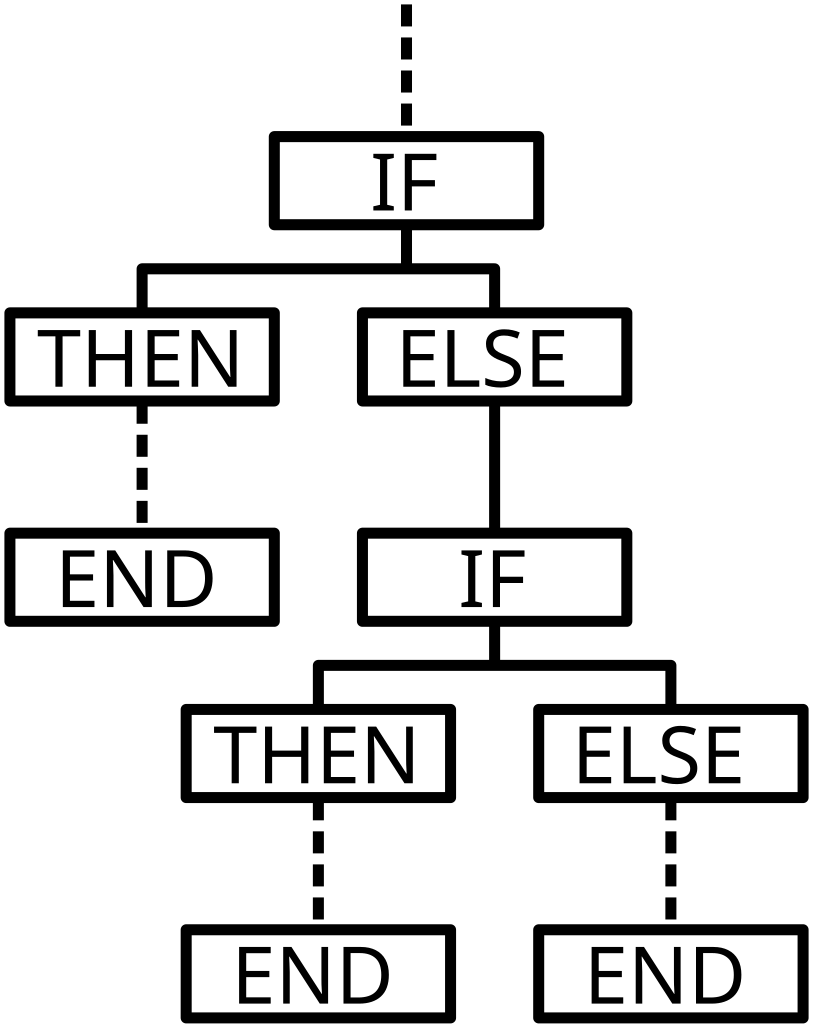
\includegraphics{elif}
  \caption{Flowchart of the \lstinline{if}, \lstinline{elif}, and \lstinline{else} construct}
  \labfig{elif}
\end{marginfigure}

If the command in the \lstinline{if} statement is not successful, we can run another command using the \lstinline{elif} keyword and decide the branching based on its exit status.

\begin{lstlisting}[language=bash]
$ read -p "Enter a number: " num
Enter a number: 0
$ if [[ $num -gt 0 ]] ; then
>   echo "The number is positive"
> elif [[ $num -lt 0 ]] ; then
>   echo "The number is negative"
> else
>   echo "The number is zero"
> fi
The number is zero
\end{lstlisting}

Here we have added an \lstinline{elif} statement to check if the number is less than 0, and if it is, we print that the number is negative, finally if both the commands are unsuccessful, we execute the statements in the \lstinline|else| block.

\section{Exit code inversion}

We can also invert the condition using the \lstinline{!} operator.

\begin{lstlisting}[language=bash]
$ var=apple
$ if ! [ "$var" = "banana" ] ; then
>   echo "The variable is not banana"
> fi
The variable is not banana
\end{lstlisting}

\section{Mathematical Expressions as if command}

We can also use the \lstinline{((} keyword to evaluate mathematical expressions in the \lstinline{if} statement. This environment does not print any output to the standard output, rather, it exits with a zero exit code if the result of the mathematical evaluation is non-zero, and exits with a non-zero exit code if the evaluation results to zero. This is useful as $0$ is false in mathematics but $0$ is success exit code in the shell.

\begin{lstlisting}[language=bash]
$ if (( 5 > 3 )) ; then
>   echo "5 is greater than 3"
> fi
5 is greater than 3
\end{lstlisting}

However, this environment only supports integers, and not floating point numbers.

\section{Command Substitution in if}

We can also run a command in the \lstinline{if} statement, and compare the output of the command to a value using the \lstinline|test| command and the \lstinline|$(())| construct.

\begin{lstlisting}[language=bash]
$ if [ $(wc -l < file.txt) -gt 100 ] ; then
>   echo "The file is big"
> fi
The file is big
\end{lstlisting}

\section{Switch}

\begin{definition}[Switch Case]
  A switch case is a syntactical sugar that helps match a variable's value against a list of options (or patterns) and executes the block of code corresponding to the match.
\end{definition}

The branching achieved by \textbf{switch case} can also be achieved by using multiple \lstinline{if-elif-else} statements, but the switch case is more readable and concise.

\textbf{Syntax}

\marginnote{
  The \lstinline|case| block is ended with the keyword \lstinline|esac|, which is the reverse of the \lstinline|case| keyword.
}
\begin{lstlisting}[language=bash]
case var in
  pattern1)
    # code to execute if var matches pattern1
    ;;
  pattern2)
    # code to execute if var matches pattern2
    ;;
  *)
    # code to execute if var does not match any pattern
    ;;
esac
\end{lstlisting}

The \lstinline{case} keyword is followed by the variable to match against, and the \lstinline{in} keyword.
Then we have multiple patterns, each followed by a block of code to execute if the variable matches the pattern.

The \lstinline{;;} keyword is used to denote the end of a block of code, and the start of the next pattern. This ensures that the script does not continue running the statements of the other blocks after it as well.

The \lstinline{*} pattern is a wildcard pattern, and matches any value that does not match any of the other patterns.

The patterns in the switch case are similar to globs rather than regular expressions, so we cannot use regular expressions in the switch case.

Although sometimes we actually want to execute the blocks after the match. This is called fall through.

\subsection{Fall Through}

If we replace the \lstinline|;;| with \lstinline|;&| or \lstinline|;;&| then the control will flow into the next block.

\marginnote{
  In this example, the script will print both the statements "Multiple of 10" and "Multiple of 5" for numbers ending with zero because of the fall through \lstinline|;&| instead of \lstinline|;;|.
}
\begin{lstlisting}[language=bash]
$ cat switch.sh
read -p "Enter number: " num
case "$num" in
  *0) echo "Multiple of 10" ;&
  *5) echo "Multiple of 5" ;;
  *) echo "Not Multiple of 5" ;;
esac
$ bash switch.sh
Enter number: 60
Multiple of 10
Multiple of 5
\end{lstlisting}

\subsection{Multiple Patterns}

We can also have multiple patterns for a single block of code by separating the patterns with the \lstinline{|} operator.

\begin{lstlisting}[language=bash]
$ cat switch.sh
read -p "Enter digit: " num
case "$num" in
  1|2|3) echo "Small number" ;;
  4|5|6) echo "Medium number" ;;
  7|8|9) echo "Large number" ;;
  *) echo "Invalid number" ;;
esac
$ bash switch.sh
Enter digit: 5
Medium number
\end{lstlisting}

\section{Select Loop}

\begin{definition}[Select Loop]
  A select loop is a construct that is used to create a menu in the shell script. It takes a list of items and displays them to the user, and then waits for the user to select an item. The selected item is stored in a variable, and the block of code corresponding to the selected item is executed.
  This repeats infinitely, until the user stops it.
\end{definition}

\begin{lstlisting}[language=bash]
$ cat select.sh
select choice in dog cat bird stop
do
  case $choice in
    dog) echo "A dog barks" ;;
    cat) echo "A cat meows" ;;
    bird) echo "A bird chirps" ;;
    stop) break ;;
    *) echo "Invalid choice" ;;
  esac
done
$ bash select.sh
1) dog
2) cat
3) bird
4) stop
#? 1
A dog barks
#? 2
A cat meows
#? 3
A bird chirps
#? 4
\end{lstlisting}

A select loop is simply a syntactical sugar for a while loop that displays a menu to the user and waits for the user to select an option and reads it using \lstinline|read|.
The conditional branching is done using a \lstinline|case| statement.

The menu output is actually displayed on the standard error stream, so that it is easy to split the conditional output from the menu output.

\begin{lstlisting}[language=bash]
$ bash select.sh > output.txt
1) dog
2) cat
3) bird
4) stop
#? 1
#? 2
#? 3
#? 4
$ cat output.txt
A dog barks
A cat meows
A bird chirps
\end{lstlisting}

To stop the select loop, we can use the \lstinline|break| keyword.
We will see more about loops in the next section.

\section{Loops}

If we want to execute a block of code multiple times, we can use loops. There are three types of loops in bash:

\begin{itemize}
    \item \textbf{For loop} - Used to iterate over a list of items or a fixed number of times
    \item \textbf{While loop} - Used to execute a block of code as long as a condition is true
    \item \textbf{Until loop} - Used to execute a block of code as long as a condition is false
\end{itemize}

\subsection{For loop}

In bash, we can use the \lstinline{for} loop to iterate over a list of items,
called a \textbf{for-each} loop
\sidenote{
This is similar to how the for loop in Python works.
}, or a range of numbers
\sidenote{
This is similar to how the for loop in C and C like languages works.
}.

\subsubsection{For-each loop}

\begin{lstlisting}[language=bash]
$ cat foreach.sh
for item in mango banana strawberry; do
  echo "$item shake"
done
$ bash foreach.sh
mango shake
banana shake
strawberry shake
\end{lstlisting}

As we saw in \refch{variables}, there are three ways to iterate over an array in bash.
We can either treat the entire array as a single element (\lstinline|"${arr[*]}"|),
we can break the elements by spaces (\lstinline|${arr[@]}|),
or we can split as per the array elements, preserving multi-word elements (\lstinline|"${arr[@]}"|).

\textbf{Treating entire array as a single element:}
\begin{lstlisting}[language=bash]
$ cat forsplit.sh
name=("Sayan" "Alice" "John Doe")
for name in "${name[*]}"; do
  echo "Name: $name"
done
$ bash forsplit.sh
Name: Sayan Alice John Doe
\end{lstlisting}

\textbf{Splitting by spaces:}

\begin{lstlisting}[language=bash]
$ cat forsplit.sh
name=("Sayan" "Alice" "John Doe")
for name in ${name[@]}; do
  echo "Name: $name"
done
$ bash forsplit.sh
Name: Sayan
Name: Alice
Name: John
Name: Doe
\end{lstlisting}

\textbf{Preserving multi-word elements:}

\begin{lstlisting}[language=bash]
$ cat forsplit.sh
name=("Sayan" "Alice" "John Doe")
for name in "${name[@]}"; do
  echo "Name: $name"
done
$ bash forsplit.sh
Name: Sayan
Name: Alice
Name: John Doe
\end{lstlisting}

We can also dynamically generate a list of numbers in a range using the \lstinline|{start..end}| syntax or the \lstinline|seq| command.

\begin{lstlisting}[language=bash]
$ cat range.sh
for i in {1..5}; do
  echo "Number: $i"
done
$ bash range.sh
1
2
3
4
5
\end{lstlisting}

\begin{lstlisting}[language=bash]
$ cat range.sh
for i in $(seq 1 5); do
  echo "Number: $i"
done
$ bash range.sh
1
2
3
4
5
\end{lstlisting}

\textbf{Differences between range expansion and seq command}

Although both \lstinline|seq| and the \textbf{range expansion} bash syntax have similar functionality, they have slightly different behaviour, as seen in \reftab{rangevsseq}.

\begin{table*}[h!]
  \caption{Differences between range expansion and seq command}
  \labtab{rangevsseq}
  \begin{tabular}{l l}
    \toprule
    \textbf{Range Expansion} & \textbf{Seq Command} \\
    \midrule
    It is a bash feature hence it is faster & It is an external command \\
    Only integer step size & Fractional step size is allowed \\
    Works on letters & Works only on numbers \\
    Step size should be the third argument & Step size should be the second argument \\
    Output is space separated & Output is newline separated \\
    Start range cannot be omitted & Start range is 1 by default \\
    \bottomrule
  \end{tabular}
\end{table*}

\textbf{Letters:}

\begin{lstlisting}[language=bash]
$ echo {a..e}
a b c d e
$ seq a e
seq: invalid floating point argument: 'a'
Try 'seq --help' for more information.
\end{lstlisting}

\textbf{Position of step size:}

\begin{lstlisting}[language=bash]
$ echo {1..10..2}
1 3 5 7 9
$ seq 1 2 10
1
3
5
7
9
\end{lstlisting}

\textbf{Fractional step size:}

\marginnote{
  Note that if the shell is not able to expand a range expansion due to invalid syntax it will not throw an error, rather it will simply keep it unexpanded. This is similar to how path expansion works.
}
\begin{lstlisting}[language=bash]
$ seq 1 0.5 2
1.0
1.5
2.0
$ echo {1..2..0.5}
{1..2..0.5}
\end{lstlisting}

\textbf{Default start range:}

\begin{lstlisting}[language=bash]
$ seq 5
1
2
3
4
5
\end{lstlisting}

\subsubsection{Different between python's range and seq command:}

The \lstinline|seq| command is similar to the \lstinline|range| function in Python, but there are some differences between the two.

\begin{table*}[h!]
  \caption{Differences between seq and python's range function}
  \labtab{seqvspyrange}
  \begin{tabular}{l l}
    \toprule
    \textbf{Python's Range} & \textbf{Seq Command} \\
    \midrule
    Start of range is 0 by default & Start range is 1 by default \\
    Order of parameters is start,end,step & Order of parameters is start,step,end \\
    End range is exclusive & End range is inclusive \\
    \bottomrule
  \end{tabular}
\end{table*}

\subsection{C style for loop}

Bash also supports C-style for-loops, where we declare a variable, a condition for the loop, and an increment command.

\begin{lstlisting}[language=bash]
$ cat cstyle.sh
for ((i=0; i<5; i++)); do
  echo "Number: $i"
done
$ bash cstyle.sh
Number: 0
Number: 1
Number: 2
Number: 3
Number: 4
\end{lstlisting}

We can also have multiple variables in the C-style for loop.

\begin{lstlisting}[language=bash]
$ cat cstyle.sh
begin1=1
begin2=10
finish=10
for (( a=$begin1, b=$begin2; a < $finish; a++, b-- )); do
  echo $a $b
done
$ bash cstyle.sh
1 10
2 9
3 8
4 7
5 6
6 5
7 4
8 3
9 2
\end{lstlisting}

\subsection{IFS}

By default the for loop splits the input by tabs, spaces, and newlines. We can change the delimiter by changing the \lstinline|IFS| variable.

\begin{definition}[IFS]
  The \lstinline|IFS| variable is the Internal Field Separator, and is used to split the input into fields.
\end{definition}

It is used by for loop and other word splitting operations in bash.

Default value of \lstinline|IFS| is \lstinline|$' \t\n'|.
If set to multiple characters, it will split the input by any of the characters.
\sidenote{
  The \lstinline|$''| syntax is used to denote ANSI escape sequences in the string in bash.
}

\marginnote{
  In this example we are reading the \lstinline|$PATH| variable, which is a colon separated list of directories. We are changing the \lstinline|IFS| variable to a colon, so that the for loop splits the input by colon.
}
\begin{lstlisting}[language=bash]
$ cat ifs.sh
IFS=:
for i in $PATH; do
  echo $i
done
$ bash ifs.sh
/usr/local/sbin
/usr/local/bin
/usr/bin
\end{lstlisting}

We should remember to reset the \lstinline|IFS| variable after using it, as it can cause unexpected behaviour in other parts of the script.

\begin{lstlisting}[language=bash]
$ cat unsetifs.sh
IFS=:
# some code

var="a b c:d"
for i in $var; do
  echo $i
done
$ bash unsetifs.sh
a b c
d
\end{lstlisting}

Although we wanted to iterate over the elements by spliting by space, we ended up splitting by colon because we forgot to reset the \lstinline|IFS| variable.

To reset the \lstinline|IFS| variable, we can simply unset it.

\begin{lstlisting}[language=bash]
$ cat unsetifs.sh
IFS=:
# some code

unset IFS
var="a b c:d"
for i in $var; do
  echo $i
done
$ bash unsetifs.sh
a
b
c:d
\end{lstlisting}

Unsetting the \lstinline|IFS| variable will reset it to the default value of \lstinline|$' \t\n'|.

However, setting and resetting the \lstinline|IFS| variable can be cumbersome, so we can use a subshell to change the \lstinline|IFS| variable only for the for loop.

\begin{lstlisting}[language=bash]
$ cat subshellifs.sh
var="a b c:d"
(
IFS=:
for i in $var; do
  echo $i
done
)

for i in $var; do
  echo $i
done
$ bash subshellifs.sh
a b c
d
a
b
c:d
\end{lstlisting}

\subsection{While loop}

The \lstinline{while} loop is used to execute a block of code as long as a condition is true.
This is useful if we do not know the number of iterations beforehand, rather we know the condition that should be satisfied.

Just like the \lstinline{if} statement, the \lstinline{while} loop also takes a command, and executes the block of code if the command is successful.
This means we can run any arbritary command in the \lstinline{while} loop condition checking.

\begin{lstlisting}[language=bash]
$ cat while.sh
i=5
while [ $i -gt 0 ]; do
  echo  "i is $i"
  ((i--))
done
$ bash while.sh
i is 5
i is 4
i is 3
i is 2
i is 1
\end{lstlisting}

Here we are using the \lstinline|test| command to check if the variable \lstinline|i| is greater than 0, and if it is, we print the value of \lstinline|i| and decrement it by 1.

However, \lstinline|test| is not the only command that we can use in the \lstinline{while} loop condition.

\marginnote{
  Here we are using the \lstinline|grep| command to check if the password contains any special character or not, and looping as long as the user enters a strong password.\\\\
  Ideally when reading passwords, we should use the \lstinline|read -s| command to hide the input from the user, however it is ommited from the example so that the input can be seen by the reader.
}
\begin{lstlisting}[language=bash]
$ cat pass.sh
read -p "Enter password: " pass

while ! grep -q '[[:punct:]]' <<< "$pass" ; do
  echo "Password must contain at least one special character"
  read -p "Enter password: " pass
done
echo "Password is set"
$ bash pass.sh
Enter password: 123
Password must contain at least one special character
Enter password: abc
Password must contain at least one special character
Enter password: sayan
Password must contain at least one special character
Enter password: $ayan
Password is set
\end{lstlisting}

\subsection{Until loop}

The \lstinline{until} loop is used to execute a block of code as long as a condition is false.
This is simply a negation of the \lstinline{while} loop.
It is a syntactical sugar.
The last example we saw in the \lstinline{while} loop can be rewritten using the \lstinline{until} loop to omit the \lstinline|!| symbol.

\begin{lstlisting}[language=bash]
$ cat pass.sh
read -p "Enter password: " pass

until grep -q '[[:punct:]]' <<< "$pass" ; do
  echo "Password must contain at least one special character"
  read -p "Enter password: " pass
done
echo "Password is set"
$ bash pass.sh
Enter password: 123
Password must contain at least one special character
Enter password: abc
Password must contain at least one special character
Enter password: sayan
Password must contain at least one special character
Enter password: $ayan
Password is set
\end{lstlisting}

\subsection{Read in while}

The \lstinline{read} command is used to read one line of input from the user,
however if we want to read multiple lines of input,
and we do not know the number of lines beforehand,
we can use the \lstinline{while} loop to read input until the user enters a specific value,
or the input stops.
\sidenote{
  The end of input is denoted by the \lstinline|EOF| character,
  if we are reading input from standard input, we can press \lstinline|Ctrl+D| to send the \lstinline|EOF| character and mark the end of input.
}

\begin{lstlisting}[language=bash]
$ cat read.sh
while read line; do
  echo "Line is $line"
done
$ bash read.sh
hello
Line is hello
this is typed input
Line is this is typed input
now press ctrl+D
Line is now press ctrl+D
\end{lstlisting}

We can also read from a file using the \lstinline{<} operator.
Since the entire while loop is a command, we can use the \lstinline{<} operator to redirect the input to the while loop after the ending \lstinline|done| keyword.

\marginnote{
  Here we are reading the \lstinline|/etc/passwd| file line by line and printing the username.
  The username is the first field in the \lstinline|/etc/passwd| file, which is separated by a colon.
  The username is extracted by removing everything after the first colon using shell variable manipulation.
}
\begin{lstlisting}[language=bash]
$ cat read.sh
while read line; do
  echo ${line%%:*}
done < /etc/passwd
$ bash read.sh
root
bin
daemon
mail
ftp
http
nobody
dbus
systemd-coredump
systemd-network
\end{lstlisting}

We can also use the \lstinline{IFS} variable to split each row by a colon, and extract the username.

\marginnote{
  In this example, we are setting the IFS only for the while loop, and it gets reset after the loop.
  If we provide multiple variables to the \lstinline|read| command, it will split the input by the \lstinline|IFS| variable and assign the split values to the variables.
}
\begin{lstlisting}[language=bash]
$ cat read.sh
while IFS=: read username pass uid gid gecos home shell; do
  echo $username - ${gecos:-$username}
done < /etc/passwd
$ bash read.sh
root - root
bin - bin
daemon - daemon
mail - mail
ftp - ftp
http - http
nobody - Kernel Overflow User
dbus - System Message Bus
systemd-coredump - systemd Core Dumper
systemd-network - systemd Network Management
\end{lstlisting}

If the number of variables provided to the \lstinline|read| command is less than the number of fields in the input, the remaining fields are stored in the last variable.
This can be utilized to read only the first field of the input, and discard the rest.

\marginnote{
  In this example, we are reading only the first field of the input, and discarding the rest.
  In bash (and many other languages) the underscore variable is used to denote a variable that is not to be used.
}
\begin{lstlisting}[language=bash]
$ cat read.sh
while IFS=: read username _; do
  echo $username
done < /etc/passwd
$ bash read.sh
root
bin
daemon
mail
ftp
http
nobody
dbus
systemd-coredump
systemd-network
\end{lstlisting}

\subsection{Break and Continue}

The \lstinline{break} and \lstinline{continue} keywords are used to control the flow of the loop.

\begin{itemize}
    \item \textbf{Break} - The \lstinline{break} keyword is used to exit the loop immediately. This skips the current iteration, and also all the next iterations.
    \item \textbf{Continue} - The \lstinline{continue} keyword is used to skip the rest of the code in the loop and go to the next iteration.
\end{itemize}

\subsubsection{Break:}
\begin{lstlisting}[language=bash]
$ cat pat.sh
for i in {1..5}; do
  for j in {1..5}; do
    if [[ "$j" -eq 3 ]]; then
      break;
    fi
    echo -n $j
  done
  echo
done
$ bash pat.sh
12
12
12
12
12
\end{lstlisting}

\subsubsection{Continue:}
\begin{lstlisting}[language=bash]
$ cat pat.sh
for i in {1..5}; do
  for j in {1..5}; do
    if [[ "$j" -eq 3 ]]; then
      continue;
    fi
    echo -n $j
  done
  echo
done
$ bash pat.sh
1245
1245
1245
1245
1245
\end{lstlisting}

Unlike most languages, the \lstinline{break} and \lstinline{continue} keywords in bash also takes an optional argument.
This argument is the number of loops to break or continue.
If we change the \lstinline{break} keyword to \lstinline{break 2}, it will break out of the outer loop, and not just the inner loop.

\begin{lstlisting}[language=bash]
$ cat pat.sh
for i in {1..5}; do
  for j in {1..5}; do
    if [[ "$j" -eq 3 ]]; then
      break 2;
    fi
    echo -n $j
  done
  echo
done
$ bash pat.sh
12
\end{lstlisting}

The same works for the \lstinline{continue} keyword as well.

\begin{lstlisting}[language=bash]
$ cat pat.sh
for i in {1..5}; do
  for j in {1..5}; do
    if [[ "$j" -eq 3 ]]; then
      continue 2;
    fi
    echo -n $j
  done
  echo
done
$ bash pat.sh
1212121212
\end{lstlisting}

\section{Functions}

If the script is too long, it is usually better to split the script into multiple concise functions that does only one task.

There are three ways to define a function in bash:

\textbf{Without the function keyword:}

\begin{lstlisting}[language=bash]
abc(){
  commands
}
\end{lstlisting}

\textbf{function keyword with brackets}

\begin{lstlisting}[language=bash]
function abc(){
  commands
}
\end{lstlisting}

\textbf{function keyword without brackets}

\begin{lstlisting}[language=bash]
function abc {
  commands
}
\end{lstlisting}

\textbf{Example:}

\begin{lstlisting}[language=bash]
$ cat functions.sh
sayhi(){
    echo "Hello, $1"
}

sayhi "John"
$ bash functions.sh
Hello, John
\end{lstlisting}

\subsubsection{Arguments in Functions}

Just like we can use \lstinline|$1| inside a script to refer to the first argument, we can use \lstinline|$1| inside a function to refer to the first argument passed to the function.

The arguments passed to the script are not available inside the function, instead the arguments passed to the function are available inside the function.

\begin{lstlisting}[language=bash]
$ cat fun.sh
fun(){
  echo $1 $2
}
echo "Full name:" $1 $2
fun "Hello" "$1"
$ bash fun.sh John Appleseed
Full name: John Appleseed
Hello John
\end{lstlisting}

\subsubsection{Return value of a function}

Functions in bash do not return a value, rather they exit with a status code.
However, functions can print the value to the standard output, and the caller can capture the output of the function using command substitution.

\marginnote{
  In this example, we are creating a simple calculator script that takes two operands and an operator, and returns the result. The operator selection is done using a select loop, and the operands are read using \lstinline|read|.
  We have modularized the script by creating two functions, \lstinline|add| and \lstinline|mul|, that takes two operands and returns the result.
}
\begin{lstlisting}[language=bash]
$ cat calc.sh
add(){
  echo $(($1 + $2))
}

mul(){
  echo $(($1 * $2))
}

select operator in plus multiply ; do
  read -p "Operand 1: " op1
  read -p "Operand 2: " op2
  case "$operator" in
    plus) answer=$(add $op1 $op2) ;;
    multiply) answer=$(mul $op1 $op2) ;;
    *) echo "Invalid option" ;;
  esac
  echo "Answer is $answer"
done
$ bash calc.sh
1) plus
2) multiply
#? 1
Operand 1: 5
Operand 2: 4
Answer is 9
#? 2
Operand 1: 6
Operand 2: 3
Answer is 18
#?
\end{lstlisting}

However, sometimes we may want to return from a function as a means to exit the function early. We may also want to signal the success or failure of the function.
Both of these can be done using the \lstinline|return| shell built-in.

\marginnote{
  In this example, we have created a function that prints the numbers from 0 to the number passed to the function, but if the number passed is negative, the function returns early with a status code of 1. If the number if greater than $9$, it only prints till $9$, and then returns.
}
\begin{lstlisting}[language=bash]
$ cat return.sh
fun(){
  if [[ $1 -lt 0 ]]; then
    return 1
  fi
  local i=0
  while [[ $i -lt $1 ]]; do
    if [[ $i -gt 9 ]]; then
      echo
      return
    fi
    echo -n $i
    ((i++))
  done
  echo
}

fun 5
echo return value: $?
fun 15
echo return value: $?
fun -5
echo return value: $?
$ bash return.sh
01234
return value: 0
0123456789
return value: 0
return value: 1
\end{lstlisting}

\begin{remark}
  If no value is provided to the \lstinline|return| command, it returns the exit status of the last command executed in the function.
\end{remark}

\subsubsection{Local variables in functions}

By default, all variables in bash are global, and are available throughout the script.
Even variables defined inside a function are global, and are available outside the function.
This might cause confusion, as the variable might be modified by the function, and the modification might affect the rest of the script.

To make a variable local to a function, we can use the \lstinline|local| keyword.

\begin{lstlisting}[language=bash]
$ cat local.sh
fun(){
  a=5
  local b=10
}

fun
echo "A is $a"
echo "B is $b"
$ bash local.sh
A is 5
B is
\end{lstlisting}

\marginnote{
  If a variable is declared using the \lstinline|declare| keyword, it is global if defined outside a function and local if defined inside a function.
}
As it is seen in the example, the variable \lstinline|a| is available outside the function, but the variable \lstinline|b| is not available outside the function since it is defined using the \lstinline|local| shell built-in.

\section{Debugging}

Sometimes, especially when writing and debugging scripts, we may want to print out each line that the interpreter is executing, so that we can trace the control flow and find out any logical errors.

This can be done by setting the \lstinline|x| flag of \lstinline|bash| using \lstinline|set -x|.

\begin{lstlisting}[language=bash]
$ cat debug.sh
fun(){
  echo $(($1 + $2))
}

fun $(fun $(fun 1 2) 3) 4
$ bash debug.sh
10
\end{lstlisting}

In the above script, we are calling the \lstinline|fun| function multiple times, and it is difficult to trace the control flow.

To trace the control flow, we can set the \lstinline|x| flag using the \lstinline|set| command.

\begin{lstlisting}[language=bash]
$ cat debug.sh
set -x
fun(){
  echo $(($1 + $2))
}

fun $(fun $(fun 1 2) 3) 4
$ bash debug.sh
+++ fun 1 2
+++ echo 3
++ fun 3 3
++ echo 6
+ fun 6 4
+ echo 10
10
\end{lstlisting}

Now we can see the control flow of the script, and we can trace the execution of the script.
The \lstinline|+| is the \lstinline|PS4| prompt, which denotes that the line printed is a trace line and not real output of the script.

\begin{remark}
  The trace output of a script is printed to the standard error stream, so that it does not interfere with the standard output of the script.
\end{remark}

The \lstinline|PS4| prompt is repeated for each level of the function call, and is incremented by one for each level.
This helps us visualize the call stack and order of execution of the script.

\section{Recursion}

Just like other programming languages, bash also supports recursion.
However, since functions in bash do not return a value, it becomes terse to use recursion in bash by using command substitutions.

\begin{lstlisting}[language=bash]
fibo(){
  if [[ $1 -le 2 ]]; then
    echo 1
  else
    echo $(($(fibo $(($1-1))) + $(fibo $(($1-2)))))
  fi
}

for i in {1..10}; do
  fibo $i
done
\end{lstlisting}

In the above example, we are calculating the first ten elements of the fibonacci series using recursion.
We need to use \textbf{command substitution} to capture the output of the function, and then use \textbf{mathematical evaluation} environment to add the two values.

However, most recursive solutions, including this one, are not efficient, and are not recommended for use in bash as they will be very slow.
If we time the function with a argument of $20$, we see it takes a lot of time.

\begin{lstlisting}[language=bash]
$ time fibo 20
6765

real    0m13.640s
user    0m10.010s
sys     0m3.187s
\end{lstlisting}

An iterative solution would be much faster and efficient.

\begin{lstlisting}[language=bash]
$ cat fibo.sh
fibo(){
  declare -i a=0
  declare -i b=1
  for (( i=1; i<=$1; i++ )); do
    declare -i c=$a+$b
    a=$b
    b=$c
  done
  echo $a
}

time fibo 40
$ bash fibo.sh
102334155

real	0m0.001s
user	0m0.001s
sys	0m0.000s
\end{lstlisting}

The iterative solution is much faster and efficient than the recursive solution.

\section{Shell Arithmetic}

We have already seen the mathematical evaluation environment in bash, which is used to evaluate mathematical expressions.

\begin{lstlisting}[language=bash]
$ echo $((1 + 2))
3
\end{lstlisting}

However, the mathematical evaluation environment is limited to integer arithmetic, and does not support floating point arithmetic.

\subsection{bc}

A more powerful way to do arithmetic in bash is to use the \lstinline|bc| command.

\begin{definition}[BC]
  \lstinline|bc| is an arbitrary precision calculator language, and is used to do floating point arithmetic in bash.
\end{definition}

\begin{lstlisting}[language=bash]
$ bc <<< "1.5 + 2.5"
4.0
\end{lstlisting}

However, \lstinline|bc| by default will set the scale to 0, and will truncate the result to an integer.

\begin{lstlisting}[language=bash]
$ bc <<< "10/3"
3
\end{lstlisting}

This can be changed by setting the \lstinline|scale| variable in \lstinline|bc|.

\begin{lstlisting}[language=bash]
$ bc <<< "scale=3; 10/3"
3.333
\end{lstlisting}

We can also use the \lstinline|-l| flag to load the math library in \lstinline|bc|,
which provides more mathematical functions and also sets the scale to 20.

\begin{lstlisting}[language=bash]
$ bc -l <<< "10/3"
3.33333333333333333333
\end{lstlisting}

\lstinline|bc| can also be started in an interactive mode, which is a REPL.
\sidenote{
  \textbf{REPL} - \textbf{R}ead, \textbf{E}valuate, \textbf{P}rint, \textbf{L}oop
  is an interactive interpreter of a language.
}

\lstinline|bc| is not just a calculator, rather it is a full fledged programming language, and can be used to write scripts.

\marginnote{
  \lstinline|bc| supports all the basic arithmetic operations, and also supports the \lstinline|if| statement, \lstinline|for| loop, and \lstinline|while| loop and other programming constructs.
  It is similar to C in syntax, and is a powerful language.
}
\begin{lstlisting}[language=bash]
$ cat factorial.bc
define factorial(n) {
  if(n==1){
    return 1;
  }
  return factorial(n-1) * n;
}
$ bc factorial.bc <<< "factorial(5)"
120
\end{lstlisting}

Read the man page of \lstinline|bc| to know more about the language.

\begin{lstlisting}[language=bash]
$ man bc
\end{lstlisting}

\subsection{expr}

\begin{definition}[EXPR]
  \lstinline|expr| is a command line utility that is used to evaluate expressions.
\end{definition}

As \lstinline|expr| is a command line utility, it is not able to access the shell variables directly, rather we need to use the \lstinline|$| symbol to expand the variable with the value before passing the arguments to \lstinline|expr|.

\begin{lstlisting}[language=bash]
$ expr 1 + 2
3
\end{lstlisting}

The spaces around the operator are necessary, as \lstinline|expr| is a command line utility, and the shell will split the input by spaces.

The operand needs to be escaped or quoted if it has a special meaning in the shell.

\marginnote{
  The \lstinline|*| symbol is a special character in the shell, and is used for path expansion. If the folder is empty, then it remains as \lstinline|*|, but if the directory has files, then \lstinline|*| will expand to the  sorted list of all the files. In this example we show this by creating a file with the name as \lstinline|+|, thus $10 * 3$ actually expands to $10 + 3$ and gives the output of $13$.
}
\begin{lstlisting}[language=bash]
$ expr 10 \* 3
30
$ expr 10 '*' 3
30
$ ls
$ expr 10 * 3
30
$ touch '+'
$ expr 10 * 3
13
\end{lstlisting}

Like the mathematical environment, \lstinline|expr| exits a zero exit code if the expression evaluates to a non-zero value, and exits with a non-zero exit code if the expression evaluates to zero.

This inversion is useful in \lstinline|if| and \lstinline|while| loops.

\begin{lstlisting}[language=bash]
$ expr 5 '>' 6
0
$ echo $?
1
$ expr 5 '<' 6
1
$ echo $?
0
\end{lstlisting}

\lstinline|expr| can also be used to match regex patterns.
Unlike most other commands, the regex pattern is always anchored to the start of the string.

\marginnote{
  As seen, the regex pattern is always anchored to the start of the string. The matching is done greedily, and the maximum possible match is taken.
  \lstinline|expr| prints the length of the match, and not the match itself.
}
\begin{lstlisting}[language=bash]
$ expr hello : h
1
$ expr hello : e
0
$ expr hello : .*e
2
$ expr hello : .*l
4
\end{lstlisting}

However, if we want to actually print the match instead of the length, we can
enclose the regex pattern in escaped parentheses.

\begin{lstlisting}[language=bash]
$ expr hello : '\(.*l\)'
hell
\end{lstlisting}

Other string operations that \lstinline|expr| supports are:

\begin{itemize}
  \item \lstinline|length| - Returns the length of the string.
  \item \lstinline|index| - Returns the index of the first occurrence of the substring.
  \item \lstinline|substr| - Returns the substring of the string.
\end{itemize}

\begin{lstlisting}[language=bash]
$ expr length hello
5
\end{lstlisting}

\begin{lstlisting}[language=bash]
$ expr index hello e
2
\end{lstlisting}

\begin{lstlisting}[language=bash]
$ expr substr hello 2 3
ell
\end{lstlisting}

The index is 1 based in \lstinline|expr|, and not 0 based.
For the \lstinline|substr| command, the first argument is the string, the second argument is the starting index, and the third argument is the length of the substring.

\section{Running arbritary commands using source, eval and exec}

Just like we can use the \lstinline|source| command to run a script file in the current shell itself, we can also run any arbritary command directly using \lstinline|eval| without needing a file.

\begin{lstlisting}[language=bash]
$ eval date
Wed Jul 31 11:00:42 PM IST 2024
$ cat script.sh
echo "Hello"
$ source script.sh
Hello
$ eval ./script.sh
Hello
\end{lstlisting}

As it can run any command, it can also run a script file. But the \lstinline|source| command cannot run a command without a file.
However, this can be circumvented by using the \lstinline|/dev/stdin| file.

\begin{lstlisting}[language=bash]
$ source /dev/stdin <<< "echo Hello"
Hello
\end{lstlisting}

\begin{warn}
  We should be careful when using the \lstinline|eval| command, as it can run any arbritary command in the current shell, and can be a security risk.
\end{warn}

\subsection{exec}

Similar to the \lstinline|eval| command, the \lstinline|exec| command can also be used to run arbritary commands in the same environment without creating a new environment.
However, the shell gets replaced by the command being run, and when the command exits, the terminal closes. If the command fails to run then the shell is preserved.

\begin{exercise}
  Open a new terminal and run the command \lstinline|exec sleep 2|.
  Observe that the terminal closes after 2 seconds.
\end{exercise}


\section{Getopts}

Getopts is a built-in command in bash that is used to parse command line arguments.
It is a syntactical sugar that helps us parse command line arguments easily.

  The first argument to the \lstinline|getopts| command is the string that contains the options that the script accepts.
  The second argument is the name of the variable that will store the option that is parsed\dots
  \lstinline|getopts| reads each argument passed to the script one by one, and stores the option in the variable, and the argument to the option in the \lstinline|$OPTARG| variable.
  It needs to be executed as many times as the number of options passed to the script.
  As this number is often unknown, it is usually executed in a \lstinline|while| loop, since the \lstinline|getopts| command returns a non-zero exit code once all the passed options are checked.

\begin{lstlisting}[language=bash]
$ cat optarg.sh
while getopts ":a:bc:" flag; do
    echo "flag -$flag, Argument $OPTARG";
done
$ bash optarg.sh -a 1 -b -c 2
flag -a, Argument 1
flag -b, Argument
flag -c, Argument 2
\end{lstlisting}

The colon after the option denotes that the option requires an additional argument.
The colon at the start of the string denotes that the script should not print an error message if an invalid option is passed.

\textbf{Without the leading colon:}
\begin{lstlisting}[language=bash]
$ cat optarg.sh
while getopts "a:" flag; do
    echo "flag -$flag, Argument $OPTARG";
done
$ bash optarg.sh -a 1 -b
flag -a, Argument 1
optarg: illegal option -- b
flag -?, Argument
$ bash optarg.sh -a
optarg: option requires an argument -- a
flag -?, Argument
\end{lstlisting}

\textbf{With the leading colon:}
\begin{lstlisting}[language=bash]
$ cat optarg.sh
while getopts ":a:" flag; do
    echo "flag -$flag, Argument $OPTARG";
done
$ bash optarg.sh -a 1 -b
flag -a, Argument 1
flag -?, Argument b
$ bash optarg.sh -a
flag -:, Argument a
\end{lstlisting}

If the option is not passed, the \lstinline|$OPTARG| variable is set to the option itself, and the \lstinline|flag| variable is set to \lstinline|:|.

If an illegal option is passed, the \lstinline|flag| variable is set to \lstinline|?|, and the \lstinline|$OPTARG| variable is set to the illegal option.

These let the user print a custom error message if an illegal option is passed or if an option that requires an argument is passed without an argument.

\subsection{With case statement}

Usually the \lstinline|getopts| command is used with a \lstinline|case| statement to execute the code for each option.

\begin{lstlisting}[language=bash]
$ cat optarg.sh
time="Day"
while getopts ":n:mae" opt; do
  case $opt in
    n) name=$OPTARG ;;
    m) time="Morning" ;;
    a) time="Afternoon" ;;
    e) time="Evening" ;;
    \?) echo "Invalid option: $OPTARG" >&2 ;;
  esac
done
echo -n "Good $time"
if [ -n "$name" ]; then
  echo ", $name!"
else
  echo "!"
fi
$ bash optarg
Good Day!
$ bash optarg -a
Good Afternoon!
$ bash optarg -e
Good Evening!
$ bash optarg -m
Good Morning!
$ bash optarg -an Sayan
Good Afternoon, Sayan!
$ bash optarg -mn Sayan
Good Morning, Sayan!
$ bash optarg -en Sayan
Good Evening, Sayan!
$ bash optarg -n Sayan
Good Day, Sayan!
$ bash optarg -n Sayan -a
Good Afternoon, Sayan!
\end{lstlisting}

The error printing can also be supressed by setting the \lstinline|OPTERR| shell variable to $0$.

\section{Profile and RC files}

There are two kinds of bash environments:

\begin{itemize}
  \item \textbf{Login shell} - A login shell is a shell that is started after a user logs in. It is used to set up the environment for the user.
  \item \textbf{Non-login shell} - A non-login shell is a shell that is started after the user logs in, and is used to run commands.
\end{itemize}

When a non-login shell is started, it reads the \lstinline|~/.bashrc| file, and the \lstinline|/etc/bash.bashrc| file.
\sidenote{
  The \textbf{rc} in \textbf{bashrc} stands for \textbf{run command}.
  This is a common naming convention in Unix-like systems, where the configuration files are named with the extension \textbf{rc}.
}

When a login shell is started, along with the \textbf{run command} files, it reads the \lstinline|/etc/profile| file, and then reads the \lstinline|~/.bash_profile| and \lstinline|~/.profile| file.

We make most of the configuration changes in the \lstinline|~/.bashrc| file, as it is read by both login and non-login shells, and is the most common configuration file.
Make sure to backup the \lstinline|~/.bashrc| file before making any changes, as a misconfiguration can cause the shell to not start.

\newpage
\section{Summary}

In this chapter, we learned about the control flow constructs in bash, and how to use them to author scripts to automate your work.

\begin{table*}[h!]
  \caption{Summary of the bash constructs}
  \labtab{bash-constructs}
  \begin{tabular}{ll}
    \toprule
    \textbf{Construct} & \textbf{Description} \\
    \midrule
    \lstinline|if| & Used to execute a block of code based on a condition. \\
    \lstinline|case| & Used to execute a block of code based on a pattern. \\
    \lstinline|for| & Used to iterate over a list of elements. \\
    \lstinline|while| & Used to execute a block of code as long as a condition is true. \\
    \lstinline|until| & Used to execute a block of code as long as a condition is false. \\
    \lstinline|break| & Used to exit the loop immediately. \\
    \lstinline|continue| & Used to skip the rest of the code in the loop and go to the next iteration. \\
    \lstinline|read| & Used to read input from the user. \\
    \lstinline|unset| & Used to unset a variable. \\
    \lstinline|local| & Used to declare a variable as local to a function. \\
    \lstinline|return| & Used to return from a function. \\
    \lstinline|source| & Used to run a script file in the current shell. \\
    \lstinline|eval| & Used to run arbritary commands in the current shell. \\
    \lstinline|exec| & Used to run arbritary commands in the current shell. \\
    \lstinline|getopts| & Used to parse command line arguments. \\
    \bottomrule
  \end{tabular}
\end{table*}

% \chapter{Stream Editor}
\labch{sed}

\begin{marginfigure}
  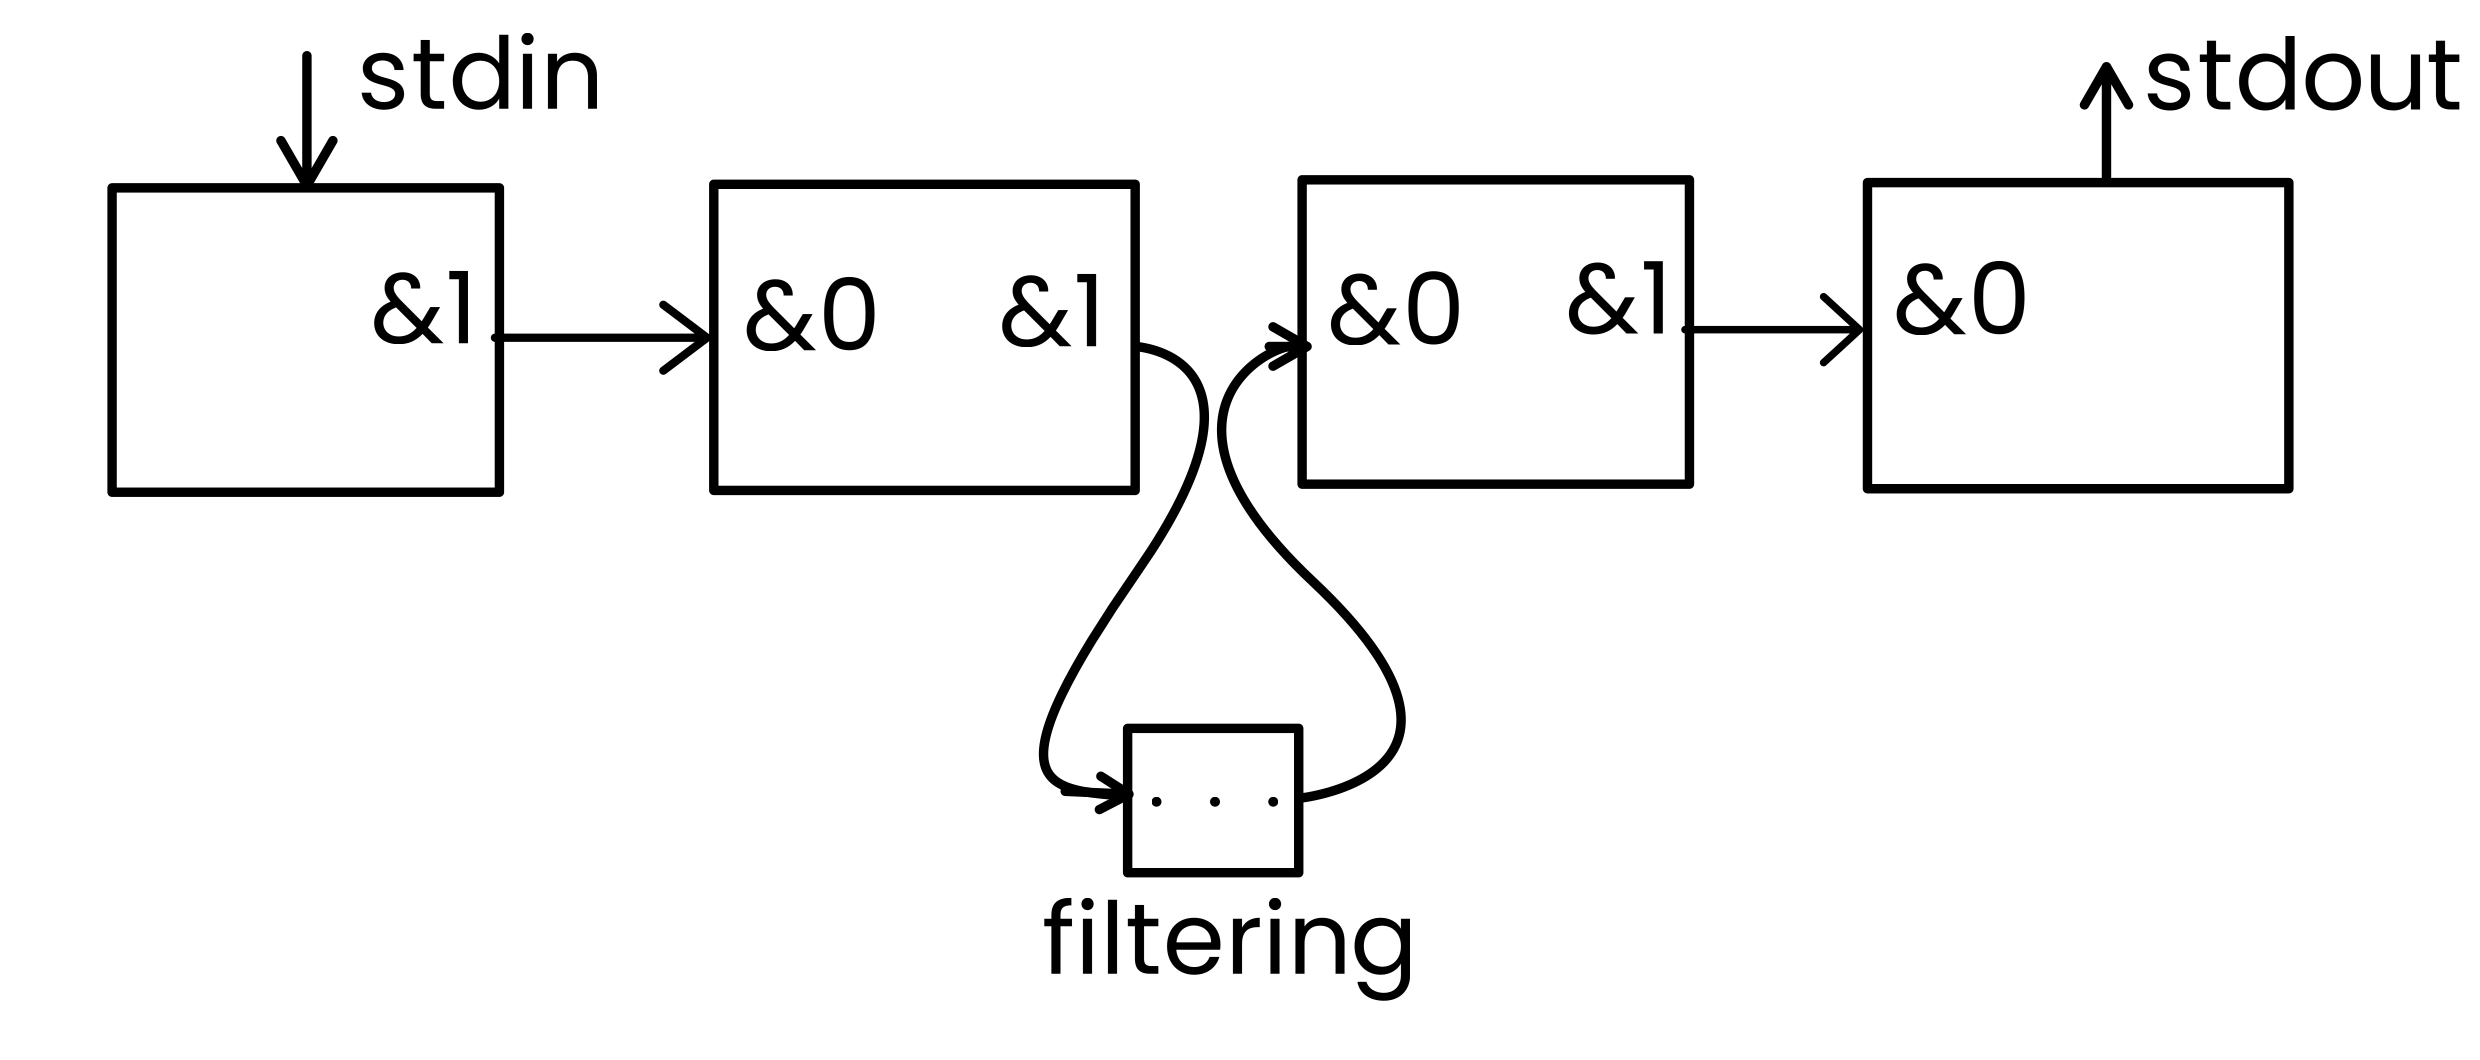
\includegraphics{filtering}
  \caption{Filtering Streams}
  \labfig{filtering}
\end{marginfigure}

\textbf{Stream Editor} (sed) is a powerful text stream editor. It is used to perform basic text transformations on an input stream (a file or input from a pipeline). While in some ways similar to an editor which permits scripted edits (such as ed), sed works by making only one pass over the input(s), and is consequently more efficient. But it is sed's ability to filter text in a pipeline which particularly distinguishes it from other types of editors.

This means that sed can be used in a pipeline of other commands to filter, refine, and transform the data in the stream. This is illustrated in \reffig{filtering}.

\begin{remark}
\lstinline|sed| is short for \textbf{S}tream \textbf{ED}itor.
\end{remark}

\section{Basic Usage}

\begin{marginfigure}[-3cm]
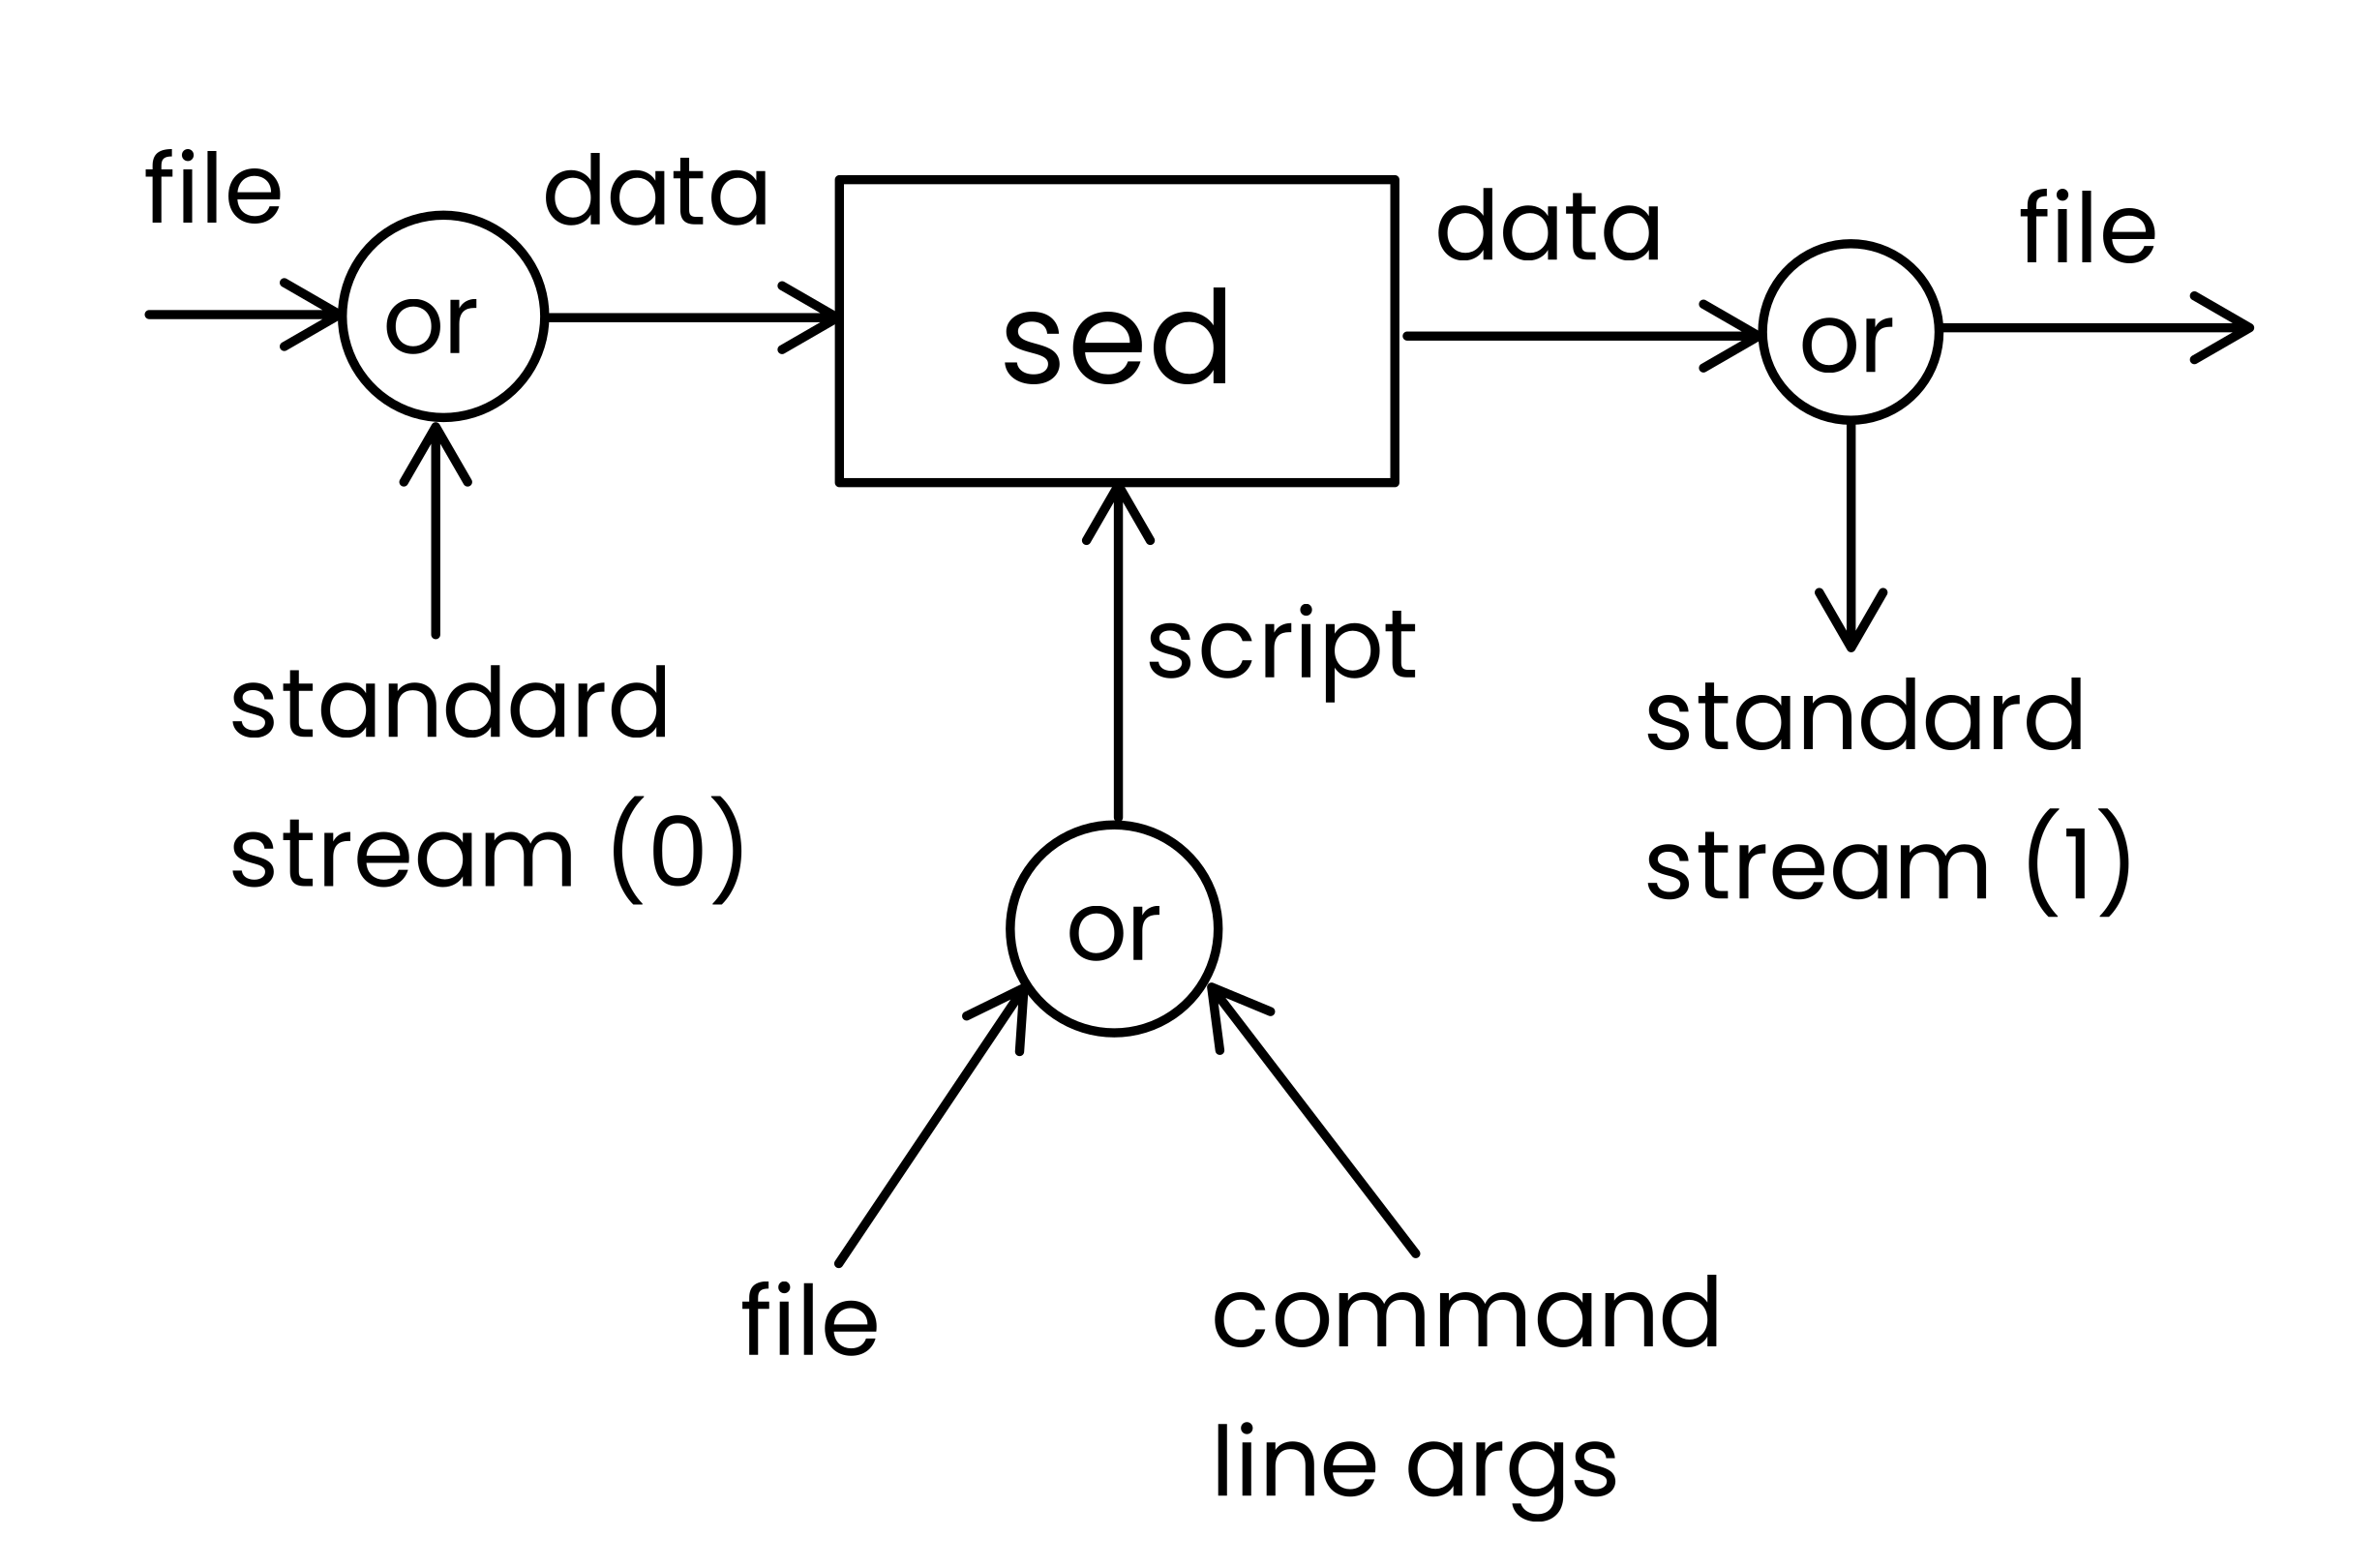
\includegraphics{sed}
\caption{The different interfaces to sed}
\labfig{sed}
\end{marginfigure}

Sed needs an input (stream or file) and a script to work. The script is a series of commands that sed will execute on the input. The script can be passed as a command line argument or as a file as well.

For example, we can provide the stream to manipulate as standard input, and provide a single command as the script directly through the command line.

\marginnote{
  Here we are using the \lstinline|s| command of sed to perform a find-and-replace style substitution. This is similar to the \lstinline|\%s/regex/string/| present in \lstinline|vim|.
  The first argument can be a regex, but the second argument has to be a string, however it may contain backreferences to the matched pattern.
}
\begin{lstlisting}[language=bash]
$ sed 's/World/Universe/' <<< "Hello World"
Hello Universe
\end{lstlisting}

As sed can work on standard input if no file is provided, it is very useful when paired with other tools; It can transform or filter output of commands.

For example, the default output of date does not zero-pad the date.
If we want to do that using \lstinline|sed|, we can do it as follows:

\marginnote{
  This does not add an extra zero if the date is already two digits long.
  As we have already covered regular expressions in depth, it should be easy to understand the regex used here. We are grouping the regex to use it in the back reference and add an extra zero if the date is a single digit.
}
\begin{lstlisting}[language=bash]
$ date
Tue Aug  6 05:00:23 PM IST 2024
$ date | sed -E 's/^([[:alpha:]]*[[:space:]]*[[:alpha:]]*)[[:space:]]*([[:digit:]])[[:space:]]/\1 0\2 /'
Tue Aug 06 05:00:32 PM IST 2024
$ date -d "20241225"
Wed Dec 25 12:00:00 AM IST 2024
$ date -d "20241225" | sed -E 's/^([[:alpha:]]*[[:space:]]*[[:alpha:]]*)[[:space:]]*([[:digit:]])[[:space:]]/\1 0\2 /'
Wed Dec 25 12:00:00 AM IST 2024
\end{lstlisting}

If the pattern being searched does not match on the input, sed will not make any changes to the input.

\section{Addressing}

All of the commands in \lstinline|sed| runs on all the lines by default.
However, we can specify the lines to run on by providing the optional address field before the command.

\begin{lstlisting}[language=bash]
$ cat data
hello world
hello universe
$ sed '1s/hello/hi/' data
hi world
hello universe
\end{lstlisting}

The address can be the line number of a particular line, range of line numbers, or a regex pattern to match. We can also use \lstinline|$| to match the last line and \lstinline|1| to match the first line.

\begin{lstlisting}[language=bash]
$ seq 10 20 | sed '5,10d'
10
11
12
13
20
\end{lstlisting}

\begin{lstlisting}[language=bash]
$ seq 10 20 | sed '/15/,/20/d'
10
11
12
13
14
\end{lstlisting}

\begin{lstlisting}[language=bash]
$ seq 10 20 | sed '5d'
10
11
12
13
15
16
17
18
19
20
\end{lstlisting}


Furthermore, we can also specify the range of addresses to run the command on, using regex as the start, end, or both the ends.

\begin{lstlisting}[language=bash]
$ seq 10 20 | sed '/13/,$d'
10
11
12
\end{lstlisting}

The range usually uses the start and end addresses separated by a comma. But we can also use \lstinline|+n| to include \lstinline|n| lines starting from the start range.

\begin{lstlisting}[language=bash]
$ seq 10 20 | sed '/13/,+5d'
10
11
12
19
20
\end{lstlisting}

To match every \lstinline|n|th line, we can use \lstinline|~n|.

\begin{lstlisting}[language=bash]
$ seq 10 20 | sed '0~2d'
10
12
14
16
18
20
\end{lstlisting}

\subsection{Negation}

We can negate the address by using the \lstinline|!| operator before the address.

\begin{lstlisting}[language=bash]
$ seq 8 5 32 | sed '/1./!d'
13
18
\end{lstlisting}

In this example we first use the \lstinline|seq| command to generate a sequence of numbers from 8 to 32 with a step of 5.
Then we use \lstinline|sed| to delete all the lines that do not match the pattern \lstinline|1.|, printing only the numbers that start with $1$.

\section{Commands}

\subsection{Command Syntax}

The general syntax of the sed command is as follows:

\begin{lstlisting}[language=bash]
[:label] [address] command [arguments]
\end{lstlisting}

\subsection{Available Commands}

Sed has a lot of commands that can be used to manipulate the input stream. Here are some of the most commonly used commands:

\begin{itemize}
  \item \lstinline|p| - Print the pattern space.
  \item \lstinline|d| - Delete the pattern space.
  \item \lstinline|s| - Substitute the pattern using regex match with string. \\
    \lstinline|[address]s/search regex/replace string/[flags]|
  \item \lstinline|=| - Print the current line number.
  \item \lstinline|#| - Comment.
  \item \lstinline|i| - Insert text before the current line.
  \item \lstinline|a| - Insert text after the current line.
  \item \lstinline|c| - Change the current line.
  \item \lstinline|y| - Transliterate the characters in the pattern space.
  \item \lstinline|q [exit code]| - Quit the script.
\end{itemize}

\subsection{Branching and Flow Control}
Other than these, there are other control flow commands like \lstinline|b|, \lstinline|t|, \lstinline|:|, which let us create more complex and powerful transformations with state information.

\begin{itemize}
  \item \lstinline|b label| - Branch unconditionally to label.
  \item \lstinline|:label| - Define Label for branching.
  \item \lstinline|n| - Read the next line to the pattern space.
  \item \lstinline|N| - Append the next line to the pattern space.
  \item \lstinline|t label| - Branch to label on successful substitution.
  \item \lstinline|T label| - Branch to label on failed substitution.
  \item \lstinline|w file| - Write the pattern space to file.
  \item \lstinline|r file| - Append the contents of file to the pattern space.
  \item \lstinline|h| - Copy the pattern space to the hold space.
  \item \lstinline|H| - Append the pattern space to the hold space.
  \item \lstinline|g| - Copy the hold space to the pattern space.
  \item \lstinline|G| - Append the hold space to the pattern space.
  \item \lstinline|x| - Exchange the pattern space and the hold space.
  \item \lstinline|D| - Delete the first line of the pattern space.
  \item \lstinline|P| - Print the first line of the pattern space.
\end{itemize}

More details on these commands can be found in the \lstinline|man| and \lstinline|info| pages of \lstinline|sed|.

\subsection{Printing}

The \lstinline|p| command prints a line in sed.
By default the line in pattern space is printed by default.
However this can be suppresesed using the \lstinline|-n| flag.
Thus when the \lstinline|p| command is used along with the \lstinline|-n| flag, only the lines that are explicitly printed are shown.

\begin{lstlisting}[language=bash]
$ seq 10 20 | sed -n '5p'
14
\end{lstlisting}

\subsection{Deleting}

The \lstinline|d| command deletes the line in the pattern space.
This is useful if the \lstinline|-n| flag is not used to suppress the default printing.

\marginnote{
  Here we are deleting two ranges of lines from the input stream.
  Multiple commands can be separated by a semicolon.
}
\begin{lstlisting}[language=bash]
$ seq 10 20 | sed '1,4d;6,$d'
14
\end{lstlisting}

Thus there are two ways of filtering a stream of data as seen in the last two examples:
\begin{itemize}
  \item Print only the lines that match a pattern.
  \item Delete the lines that do not match a pattern.
\end{itemize}

\begin{remark}
  If we use the \lstinline|p| command without using the \lstinline|-n| flag, the matched lines will be printed twice, and the other lines will be printed once.
\end{remark}

\begin{lstlisting}[language=bash]
$ seq 1 5 | sed '2p'
1
2
2
3
4
5
\end{lstlisting}

\subsection{Substitution}

This is one of the most widely used commands in \lstinline|sed|.
The sustitute command is used to replace a pattern with a string.
The search pattern can be a fixed string, or a regex pattern.

\begin{remark}
  \lstinline|sed| supports two types of regex: Basic and Extended.
  Perl Compatible Regular Expressions (PCRE) are not supported by \lstinline|sed|.
\end{remark}

Like the other commands, the substitution command can be used with an address to specify the lines to run on, or on all the lines.

\begin{lstlisting}[language=bash]
$ seq 8 12 | sed 's/1/one/'
8
9
one0
one1
one2
\end{lstlisting}

Observe that although the pattern \lstinline|1| is present twice in 11, it is only replaced once as the substitution command only replaces the first occurrence of the pattern in the line.

To substitute all the occurrences of the pattern in the line, we can use the \lstinline|g| option to the \lstinline|s| command.

\begin{lstlisting}[language=bash]
$ seq 8 12 | sed 's/1/one/g'
8
9
one0
oneone
one2
\end{lstlisting}

The \lstinline|g| argument stands for global, and it replaces all the occurrences of the pattern in the line.

If we want to replace only the \lstinline|n|th occurrence of the pattern, we can mention the number instead of \lstinline|g|.

\begin{lstlisting}[language=bash]
$ seq 8 12 | sed 's/1/one/2'
8
9
10
1one
12
\end{lstlisting}

Here the \lstinline|2| flag replaces the second occurrence of the pattern in the line.

Observe that the lines with only one occurrence of the pattern are not changed at all.

\begin{remark}
 If we ask \lstinline|sed| to replace the \lstinline|n|th occurrence of the pattern, and the pattern does not occur the pattern \lstinline|n| times in the line, then the line is not changed at all.
\end{remark}

\subsubsection{Case Insensitive Substitution}

If we want to perform a case insensitive substitution, we can use the \lstinline|i| option to the \lstinline|s| flag.

\begin{lstlisting}[language=bash]
$ sed 's/Hello/Hi/i' <<< "hello world"
Hi world
\end{lstlisting}

\subsubsection{Backreferences}

Just like in \lstinline|grep| we can use groups and backreferences in \lstinline|sed| as well.

\begin{lstlisting}[language=bash]
$ sed 's/\([^,]*\),/\1\n/g' <<< "1,2,3,4,5"
1
2
3
4
5
\end{lstlisting}

Here we are matching each of the comma separated values and replacing them with the same value followed by a newline.
The group needs to be escaped with a backslash in BRE.
However we can use Extended Regular Expressions (ERE) to avoid this by using the \lstinline|-E| flag.

\marginnote{
  In these regex, we are matching any character except a comma greedily as long as possible, and replacing it with the same pattern followed by a newline.
}
\begin{lstlisting}[language=bash]
$ sed -E 's/([^,]*),/\1\n/g' <<< "apple,banana,cherry,donut,eclairs"
apple
banana
cherry
donut
eclairs
\end{lstlisting}

We are using groups and backreferences in this case as we are dropping the comma and replacing it with a newline.
However, if we want to preserve the entire match and add some text before or after it, we can use the \lstinline|&| backreference without explicitly grouping the entire match.

\begin{lstlisting}[language=bash]
$ sed 's/[^,]*,/&\n/g' <<< "apple,banana,cherry,donut,eclairs"
apple,
banana,
cherry,
donut,
eclairs
\end{lstlisting}

\begin{remark}
  The \lstinline|&| is a backreference to the entire match.
\end{remark}

\subsubsection{Uppercase and Lowercase}

We can use the \lstinline|\u| and \lstinline|\l| backreferences to convert the first character of what follows (usually a dynamically fetched backreference) to uppercase or lowercase.

Similarly, we can use the \lstinline|\U| and \lstinline|\L| backreferences to convert the entire string
\sidenote{
  The uppercasing or lowercasing is done till the end of the string or till the next \lstinline|\E| backreference.
}
to uppercase or lowercase.

\begin{lstlisting}[language=bash]
$ sed 's/.*/\u&/' <<< hello
Hello
\end{lstlisting}

\begin{lstlisting}[language=bash]
$ sed 's/.*/\U&/' <<< hello
HELLO
\end{lstlisting}

To reset the effect of the \lstinline|\U| or \lstinline|\L| backreference, we can use the \lstinline|\E| backreference.

\begin{lstlisting}[language=bash]
$ sed 's/\([^ ]*\) *\([^ ]*\)/\U\1 \E\u\2/' <<< "hello world"
HELLO World
\end{lstlisting}

Here we are matching two groups of non-space characters (words)
using the \lstinline|[^ ]*| regex,
separated by zero or more spaces.
Thus the first world is refered to by \lstinline|\1| and the second by \lstinline|\2|.
Then we are converting the first word to fully uppercase
using \lstinline|\U\1|,
and the first letter of the second word to uppercase,
using \lstinline|\u\2|.

To reset the effect of the \lstinline|\U| backreference, we use the \lstinline|\E| backreference.


\subsection{Print Line Numbers}

The \lstinline|=| command prints the line number of the current line.

\begin{lstlisting}[language=bash]
$ seq 7 3 19 | sed '='
1
2
3
4
5
\end{lstlisting}

Here we are using the \lstinline|seq| command to generate a sequence of numbers from 7 to 19 with a step of 3.
Then we are using \lstinline|sed| to print the line number of each line.
We use the \lstinline|-n| flag to suppress the default printing of the line.

\subsubsection{wc emulation}

Since we can print the line number of any line, we can use this to emulate the \lstinline|wc| command by printing only the line number of the last line.

\begin{lstlisting}[language=bash]
$ seq 7 3 19 | sed -n '$='
5
$ seq 7 3 19 | wc -l
5
\end{lstlisting}

\subsection{Inserting and Appending Text}

The \lstinline|i| command is used to insert text before the current line.
The \lstinline|a| command is used to append text after the current line.

\begin{lstlisting}[language=bash]
$ seq 1 5 | sed '2ihello'
1
hello
2
3
4
5
\end{lstlisting}

\begin{lstlisting}[language=bash]
$ seq 1 5 | sed '2ahello'
1
2
hello
3
4
5
\end{lstlisting}

Here we are using the \lstinline|seq| command to generate a sequence of numbers from 1 to 5.
Then we are using \lstinline|sed| to insert the text \lstinline|hello| before the second line.

If we drop the address, the text is inserted before every line.

\begin{lstlisting}[language=bash]
$ seq 1 5 | sed 'ihello'
hello
1
hello
2
hello
3
hello
4
hello
5
\end{lstlisting}

\begin{lstlisting}[language=bash]
$ seq 1 5 | sed 'ahello'
1
hello
2
hello
3
hello
4
hello
5
hello
\end{lstlisting}

We can also insert multiple lines by escaping the newline character.

\begin{lstlisting}[language=bash]
$ seq 1 5 | sed '2i\
hello\
how are you'
1
hello
how are you
2
3
4
5
\end{lstlisting}

\subsection{Changing Lines}

The \lstinline|c| command is used to change the current line.
This is sometimes more convenient that substituting the entire line.

Let's say we want to remove all the lines that contains $8$ or more digits consecutively, as these may be confidential information, and replace it with "REDACTED".

\begin{lstlisting}[language=bash]
$ cat data
Hello
This is my phone number:
9999999998
and
this is my aadhaar card number:
9999999999999998
my bank cvv is
123
$ sed -E '/[0-9]{8}/cREDACTED' data
Hello
This is my phone number:
REDACTED
and
this is my aadhaar card number:
REDACTED
my bank cvv is
123
\end{lstlisting}

Here we are addressing all the lines that contain $8$ or more digits consecutively, and replacing them with "REDACTED".
The \lstinline|[0-9]{8}| regex matches any sequence of $8$ digits.

\subsection{Transliteration}

The \lstinline|y| command is used to transliterate the characters in the pattern space.
This is similar to the \lstinline|tr| command.
However, it is not as powerful as \lstinline|tr| as it does not support ranges.

\begin{lstlisting}[language=bash]
$ sed 'y/aeiou/12345/' <<< "hello world"
h2ll4 w4rld
\end{lstlisting}

Unlike the \lstinline|tr| command, the \lstinline|y| command does not support unequal length strings.

\section{Combining Commands}

We can combine multiple commands in a single script by separating them with a semicolon.

\begin{lstlisting}[language=bash]
$ seq 10 20 | sed '1,4d;6,$d'
14
\end{lstlisting}

Here we are deleting two ranges of lines from the input stream.

However, sometimes we may want to perform multiple commands on the same address range,
this can be done by enclosing the commands in braces.

\marginnote{
  Here we are addressing the line by matching the regex \lstinline|#| which marks the start of a comment.
  Then on that address we are performing a compound command using braces.
  The first command (\lstinline|=|) prints the line number,
  and the second command (\lstinline|s|) deletes the \lstinline|#| and anything before it.
}
\begin{lstlisting}[language=bash]
$ cat data
from sys import argv, exit

def main():
    if len(argv) != 3+1: # TODO: move magic number to variable
        print("Incorrect Usage")
        exit(1)

    kloc,a,b = list(map(float, argv[1:]))
    # TODO: add adjustment factor
    return a * (kloc ** b)


if __name__ == "__main__":
    print(main())
$ sed -n '/#/{=;s/^.*# //p}' data
4
TODO: move magic number to variable
9
TODO: add adjustment factor
\end{lstlisting}

Here we are performing two actions on the matching lines.
\begin{itemize}
\item Printing the line number of the matching line.
\item Printing only the TODO comment, not the code before it.
\end{itemize}

This is a handy operation to extract TODO comments from the codebase.

Instead of using a semicolon to separate the commands and addressing each command, we are enclosing them in braces and addressing the group only once.

\section{In-place Editing}

As we saw in \reffig{sed}, \lstinline|sed| can be used to filter the lines of a file as well. We have also seen that in the examples till now.
However, we have always printed the output to the terminal.
The file remains unchanged.

However, we can use the \lstinline|-i| flag to edit the file in place.

\begin{lstlisting}[language=bash]
$ cat data
hello world
$ sed -i 's/\b[[:alpha:]]/\u&/g' data
$ cat data
Hello World
$ sed -i 's/\b[[:alpha:]]/\l&/g' data
$ cat data
hello world
\end{lstlisting}

This is useful when working with large files, as we do not have to write the output to a temporary file and then replace the original file with the temporary file.
It is also used widely to modify configuration files in-place without using programming languages.

\marginnote{
  In this example we are searching for a line in the configuration file that starts with \lstinline|LAUNCH_ICBM| and are then running a compound command.
  The command first tries to substitute \lstinline|FALSE| with \lstinline|TRUE|.
  If it was successful, it then branches to the end of the script to avoid changing it back to \lstinline|FALSE|.
  If the substitution was not successful then it tries to replace \lstinline|TRUE| with \lstinline|FALSE|.
  Thus the command toggles the boolean variable between \lstinline|TRUE| and \lstinline|FALSE|. We will cover branching in details later in the chapter.
}
\begin{lstlisting}[language=bash]
$ cat usa.conf
LAUNCH_ICBM=FALSE
$ sed -i '/^LAUNCH_ICBM/{s/FALSE/TRUE/;tx;s/TRUE/FALSE/}; :x' usa.conf
$ cat usa.conf
LAUNCH_ICBM=TRUE
$ sed -i '/^LAUNCH_ICBM/{s/FALSE/TRUE/;tx;s/TRUE/FALSE/}; :x' usa.conf
$ cat usa.conf
LAUNCH_ICBM=FALSE
\end{lstlisting}

We can also preserve the original file as a backup by providing a suffix to the \lstinline|-i| flag.

\begin{lstlisting}[language=bash]
$ cat data
hello
$ sed -i.backup 's/hello/bye/' data
$ cat data
bye
$ cat data.backup
hello
\end{lstlisting}

\section{Sed Scripts}

Instead of listing out the commands as a string in the command line, we can also provide a file of sed commands, called a sed script, where each command is delimited by a newline character instead of the semicolon character.

\begin{lstlisting}[language=bash]
$ cat script.sed
s/hello/hi
$ sed -f script.sed <<< "hello world"
hi world
\end{lstlisting}

Different commands should be present in separate lines in the sed script.

\begin{lstlisting}[language=bash]
$ cat script.sed
5p
10p
$ seq 101 120 | sed -n -f script.sed
105
110
\end{lstlisting}

\subsection{Order of Execution}

The sed script is executed for each line in the input stream.
The order of checking is as per the order of the stream, and then the order of the script, that is, for each line in the stream from top to bottom, each line of the script is executed
\sidenote{
  If the address matches
}
from top to bottom.

\begin{lstlisting}[language=bash]
$ cat script.sed
10p
5p
$ seq 10 | sed -n -f script.sed
5
10
\end{lstlisting}

Even though the script has the command to print the $10$th line before the command to print the $5$th line, the output is in the order of the stream.

However, if for a line in the stream, multiple commands in the script match, then the order of the script is followed.

\begin{lstlisting}[language=bash]
$ cat script.sed
/10/{
  p
  a Multiple of 10
}
/5\|10/{
  p
  a Multiple of 5
}
$ seq 10 | sed -n -f script.sed
5
Multiple of 5
10
10
Multiple of 10
Multiple of 5
\end{lstlisting}

In this example, we are printing the line if it is a multiple of $5$ or $10$.
The case of $5$ comes first as the order of the stream is in increasing order.

However, for the number $10$, both the conditions are satisfied, and the order of the script is followed, first the text "Multiple of 10" is printed, and then "Multiple of 5".

\begin{remark}
  Observe that the \lstinline|p| command prints the line, and the \lstinline|a| command appends text after the line. Even though the first \lstinline|a| is present before the second \lstinline|p|, still both the \lstinline|p| are printed first and then the \lstinline|a| are printed.
This is because the \lstinline|p| command prints the line immediately, but the \lstinline|a| command appends the text to the hold space, and prints it only when the next line is read.
\end{remark}

\section{Branching and Flow Control}

Sed supports branching and flow control commands to create more complex transformations using loop and if-else conditions.
However, \lstinline|sed| does not support syntax like \lstinline|if-else|, \lstinline|for|, or \lstinline|while| loops,
thus to perform these control flow operations, we have to use the branching commands.

This is similar to how high level languages are compiled to assembly language \textbf{GOTO} commands, and then to machine code.

\subsection{Labels}

Labels are used to mark a point in the script to branch to.
They themselves do not perform any action, but are used as a reference point for branching.

\begin{lstlisting}[language=bash]
$ cat script.sed
:label1
5p
:label2
10p
$ seq 10 | sed -n -f script.sed
5
10
\end{lstlisting}

\subsection{Branching}

Now that we have defined labels in our script, we can use branching to instruct sed to move the control flow to any arbritary label.

\begin{remark}
  The label can be defined before, or after the branching call
\end{remark}

There are two kinds of branching in \lstinline|sed|,

\begin{itemize}
  \item \textbf{Unconditional Branching} - the branching does not depend on success or failure of previous command.
  \item \textbf{Conditional Branching} - the branching is conditioned on the success or failure of the substitution done before the branching call.
\end{itemize}

\subsubsection{Unconditional Branching}

The \lstinline|b| command is used to branch unconditionally to a label.
This will always branch to the label and skip any command after it.

\begin{lstlisting}[language=bash]
$ cat script.sed
a Hello
bx
a World
:x
a Universe
$ sed -nf script.sed <<< "test"
Hello
Universe
\end{lstlisting}

In this example the command \lstinline|a Hello| is executed, and then the \lstinline|bx| command is executed.
So, the command \lstinline|a World| is skipped, and the control flow is moved to the label \lstinline|x|, and the command \lstinline|a Universe| is executed.

If the label is after the branch, it can be used to skip certain parts of the script.
However, if the label is before the branch, it can be used to loop over the same part of the script multiple times.
But if done using an unconditional branch, it will result in an infinite loop.

\begin{lstlisting}[language=bash]
$ cat script.sed
:x
p
bx
$ sed -nf script.sed <<< "hello"
hello
hello
hello
\end{lstlisting}
\vdots

The \lstinline|bx| command branches to the label \lstinline|x| unconditionally, and thus the command \lstinline|p| is executed multiple times.
To stop the infinite loop, we can press \lstinline|Ctrl+C|.

However, we can use a regex address to limit the number of times the loop is executed.

\begin{lstlisting}[language=bash]
$ cat script.sed
:x
s/\b[a-z]/\u&/
/\b[a-z]/bx
$ cat data
this is a long line with lots of words, we want to capitalize each first letter of a word.
$ sed -f script.sed data
This Is A Long Line With Lots Of Words, We Want To Capitalize Each First Letter Of A Word.
\end{lstlisting}

In this example, we are first declaring a branch label \lstinline|x|.
Then we are using the substitution command to capitalize the first letter of the first word,
observe that we are not using the \lstinline|g| flag to capitalize all the words.
Then we are using a regex address to check if there are any more words in the line.
Only if there are more words, we branch to the label \lstinline|x|.
Thus we are using a unconditional branch but we are conditionally branching to the label using the regex address.

This can be simplified using the \lstinline|t| command.

\subsubsection{Conditional Branching}

The \lstinline|t| command is used to branch to a label if the previous substitution was successful.

\begin{lstlisting}[language=bash]
$ cat script.sed
:x
s/\b[a-z]/\u&/
tx
$ cat data
this is a long line with lots of words, we want to capitalize each first letter of a word.
$ sed -f script.sed data
This Is A Long Line With Lots Of Words, We Want To Capitalize Each First Letter Of A Word.
\end{lstlisting}

Here we are using the \lstinline|t| command to branch to the label \lstinline|x| if the substitution was successful.
This will terminate once all the words are capitalized as in the next iteration the substitution will fail.

Thus this implementation will run one iteration more than the previous implementation since it terminates when the substitution fails inside the iteration.

\subsection{Appending Lines}

We can use the \lstinline|N| command to append the next line to the pattern space.
This will keep the same iteration cycle, but simply append the next line to the current line.
The next line is delmited from the current line by a newline character.
After processing the pattern space, the iteration cycle directly moves to the line after the appended line.

A line read normally by sed does not include the newline character at the end of the line, however, if the next line is appended to pattern space using
\lstinline|N|, then the newline character is included in the pattern space.

\begin{lstlisting}[language=bash]
$ cat script.sed
1~2N
=
$ seq 10 | sed -n -f script.sed
2
4
6
8
10
\end{lstlisting}

In this example, we are appending the next line to the pattern space for every odd line.
Then we are printing the line number of the current line.

Since we are appending the next line to the pattern space, the line number is printed for the even lines.

\begin{lstlisting}[language=bash]
$ cat script.sed
N
N
s/\n/;/g
$ seq 10 | sed -n -f script.sed
1;2;3
4;5;6
7;8;9
10
\end{lstlisting}

In this example, we are appending the next two lines to the pattern space.
Then we are replacing the newline characters with a semicolon.
Observe the \lstinline|g| flag in the substitution command, this is used to replace all the newline characters in the pattern space.

Since sed does not re-process the appended lines in the next cycle, the next line starts from $4$.

\begin{remark}
  The \lstinline|N| command terminates the script on the last line in GNU sed, but is undefined in the POSIX standard.
\end{remark}

\begin{exercise}
  Try the previous example without the \lstinline|g| flag in the substitution command. Predict the output before running it, observe and justify the output after running it.
  How many lines are printed?
  How many iteration cycles does \lstinline|sed| go through in this?
\end{exercise}

\subsection{Join Multiline Strings}

If we have a file where long lines are hard-wrapped using a \lstinline|\\| character at the end of the line, we can use the \lstinline|N| command to join the lines and recreate the real file.

\begin{lstlisting}[language=bash]
$ cat data
Hello, this is a ver\
y long line, but I h\
ave broken it into s\
everal lines of fixe\
d width and marked f\
orced breaks with a \
backwards slash befo\
re the newline chara\
cter.
Real newlines do not\
 have the backslash \
though.
Like this.
$ cat script.sed
:x
/\\$/{
  N
  s/\\\n//
  bx
}
$ sed -f script.sed data
Hello, this is a very long line, but I have broken it into several lines of fixed width and marked forced breaks with a backwards slash before the newline character.
Real newlines do not have the backslash though.
Like this.
\end{lstlisting}

In this script, we first are defining a label \lstinline|x|.
Then we are checking if the line ends with a \lstinline|\\| character.
If it does, then we are appending the next line to the pattern space.
Then we are substituting the \lstinline|\\| and the newline character with an empty string, this joins the word-wrapped lines back.
Finally, we are branching back to the label \lstinline|x| to check if the current pattern space still has a \lstinline|\\| at the end.

There are other ways of performing the same action, such as using \lstinline|t| and \lstinline|P|.

\begin{exercise}
  Try to implement the same script using the \lstinline|t| and \lstinline|P| commands.
\end{exercise}

% \chapter{AWK}
\labch{awk}

\section{What is AWK?}

Awk is programming language meant for processing structured data in rows and columns.

\begin{marginfigure}
  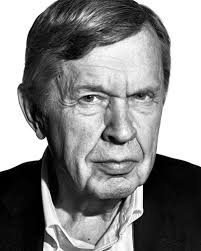
\includegraphics{aho}
  \caption{Alfred Aho}
  \labfig{aho}
\end{marginfigure}
\begin{marginfigure}
  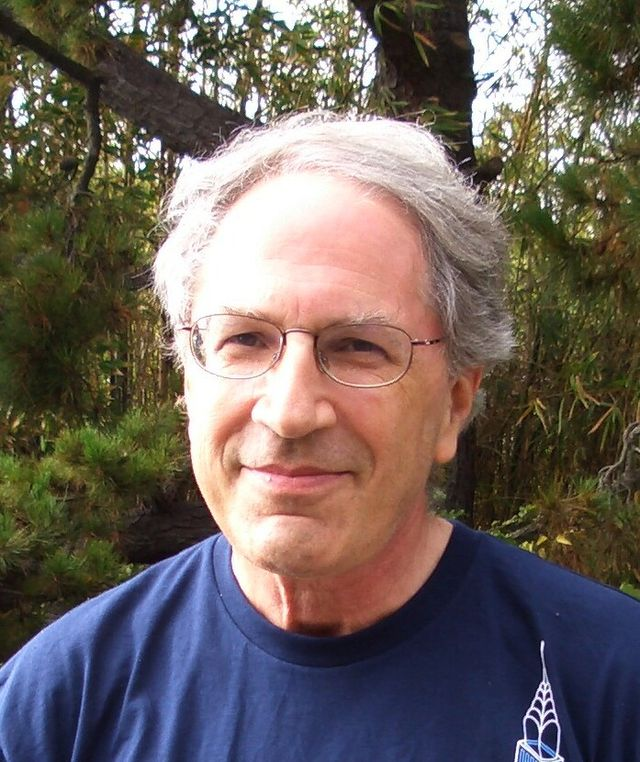
\includegraphics{weinberger}
  \caption{Peter Weinberger}
  \labfig{weinberger}
\end{marginfigure}
\begin{marginfigure}
  \includegraphics{kernighan}
  \caption{Brian Kernighan}
  \labfig{kernighan}
\end{marginfigure}

The name \textbf{AWK} comes from the initials of its creators:
\begin{itemize}
\item Afred \textbf{A}ho
\item Peter \textbf{W}einberger
\item Brian \textbf{K}ernighan
\end{itemize}

\begin{remark}
  Afred Aho was the author of \textit{egrep} and thus \textbf{awk} works with Extended Regular Expressions directly, and not Basic Regular Expressions.
\end{remark}

The most popular distribution of awk is \textbf{gawk} - GNU AWK, developed by the GNU team and distributed under the GPL.

Kernighan also released his version \textbf{nawk} - New AWK, that is used by BSD systems to avoid GPL.

AWK was the only scripting language in user space in early days along with the bourne shell. It inspired the creation of the \textbf{Perl} language which also has powerful text processing tools.

The awk language is a data-driven language, that is, it processes data line by line. It is a procedural language, but it is not object-oriented.
It has a very simple syntax, and it is very powerful for text processing.
For each line that is read, awk applies a set of rules to the line and executes the actions that are associated with the rules.

\section{Basic Syntax}

The basic syntax of an awk program is a series of pattern action pairs, written as:

\begin{lstlisting}
pattern { action }
\end{lstlisting}

The entire input is split into records, and each record is split into fields. By default records are split using newlines, so each record is one line of input, but it can be changed.

Each record is tested against the pattern, and if the pattern matches, the action is executed.

Thus, an awk program has an implicit loop that reads each record, tests each record against the patterns, and executes the actions if they match.

\marginnote{
  Here we are checking for numbers in each line and if the number ends with a $5$ then we are printing that it is a multiple of $5$. Similarly if it ends with a $0$, then we print that it is a multiple of $5$ and $10$.
  Observe how this is achieved using regex alternation and multiple pattern-action pairs.
}
\begin{lstlisting}[language=bash]
$ cat script.awk
/5$|0$/ {
  print $0 " is a multiple of 5"
}

/0$/  {
  print $0 " is a multiple of 10"
}
$ seq 20 | awk -f script.awk
5 is a multiple of 5
10 is a multiple of 5
10 is a multiple of 10
15 is a multiple of 5
20 is a multiple of 5
20 is a multiple of 10
\end{lstlisting}

If the pattern is omitted, the action is executed for every record.

\begin{lstlisting}[language=bash]
$ cat script.awk
{
  print "Line: " $0
}
$ seq 5 | awk -f script.awk
Line: 1
Line: 2
Line: 3
Line: 4
Line: 5
\end{lstlisting}

If the action is omitted, the default action is to print the record.

\begin{lstlisting}[language=bash]
$ seq 50 | awk '/5$/'
5
15
25
35
45
\end{lstlisting}

\subsection{Special Conditions}

\begin{itemize}
\item \textbf{BEGIN} - This pattern is executed before the first record is read.
\item \textbf{END} - This pattern is executed after the last record is read.
\end{itemize}

\begin{lstlisting}[language=bash]
$ cat script.awk
BEGIN{
  print "Starting the script"
}
{
  print "Line: " $0
}
END{
  print "Ending the script"
}
$ seq 5 | awk -f script.awk
Starting the script
Line: 1
Line: 2
Line: 3
Line: 4
Line: 5
Ending the script
\end{lstlisting}

\subsection{Ranges}

The condition can also be a range of records, matched by their record number or by regular expression patterns.
Both the ends are inclusive.

\textbf{Example:}

\marginnote{
  Here we are printing from the line starting with a capital T and till the line that ends with a full stop.
}
\begin{lstlisting}[language=bash]
$ cat data.txt
Hello
This is the start
of a long sentence
spanning multiple
lines in the file.
Goodbye
$ awk '/^T/,/\.$/'
This is the start
of a long sentence
spanning multiple
lines in the file.
\end{lstlisting}

The record number can be matched using the \lstinline|NR| variable. It is a variable built-in awk and it is automatically updated everytime a new record is read.

\begin{lstlisting}[language=bash]
$ seq 10 | awk 'NR == 3, NR == 7'
3
4
5
6
7
\end{lstlisting}

\subsection{Fields}

Awk splits each record into fields. By default the fields are split by any kind of whitespace, including spaces and tabs. However, this can be changed to split by some other delimiter or even regular expression. This is useful for different structured files such as CSV and quoted CSV files.

The fields are numbered from $1$ and can be accessed using the \lstinline|$i| syntax.

\begin{lstlisting}[language=bash]
$ echo "Hello World" | awk '{print $1}'
Hello
\end{lstlisting}

The variable \lstinline|$0| variable contains the entire record.

We can also match a regular expression pattern against a specific field as well using the \lstinline|~| syntax.

\begin{lstlisting}[language=bash]
$ echo -e "Hello World\nhello universe\nthis is hello" | awk '$1 ~ /[hH]ello/'
Hello World
hello universe
\end{lstlisting}

\subsection{Number of Fields and Number of Records}

The number of fields in a record can be accessed using the \lstinline|NF| variable. It is a built-in variable in awk.

\marginnote{
  Here we are printing the number of fields in each line. The number of fields may change from record to record, the variable \lstinline|NR| will also be updated accordingly automatically.
}
\begin{lstlisting}[language=bash]
$ echo "Hello World" | awk '{print NF}'
2
\end{lstlisting}

The number of records can be accessed using the \lstinline|NR| variable. It is a built-in variable in awk.

\marginnote{
  Here we are printing the \lstinline|NR| variable which is updated everytime a new record is read. Thus the \lstinline|NR| variable stores the value $i$ when it is reading the $i^{th}$ record. However, we are not printing it for each record, rather we are printing it only after all the records are read, in the \lstinline|END| block. The \lstinline|NR| variable is not wiped after reading the last record, thus it still contains the record number of the last record, which is same as the total number of records as we count from $1$.
}
\begin{lstlisting}[language=bash]
$ seq 5 10 | awk 'END{print NR}'
6
\end{lstlisting}

\subsection{Splitting Records by custom delimiter}

By default awk splits records by whitespace. However, we can change this to split by some other delimiter.
There are two variables that control this behavior:

\begin{itemize}
  \item \lstinline|FS| - Field Separator - This is the regular expression that is used to split the fields in a record.
  \item \lstinline|FPAT| - Field Pattern - This is the regular expression that is used to match the fields in a record.
\end{itemize}

The \lstinline|FS| variable can be set in the BEGIN block, or it can be set from the command line using the \lstinline|-F| option.
The \lstinline|FPAT| variable can be set in the BEGIN block.

\begin{lstlisting}[language=bash]
$ echo "Hello,World" | awk  '{print $1}'
Hello,World
$ echo "Hello,World" | awk -F, '{print $1}'
Hello
\end{lstlisting}

Here we can see that by default the record is split by whitespace, and thus the entire line is considered as a single field. However, when we set the \lstinline|FS| variable to a comma, then the record is split by the comma and we get the first field as \lstinline|Hello|.

The \lstinline|FS| variable can also be explicitly set inside the script, if for example we do not have access to the command line flags.

\begin{lstlisting}[language=bash]
$ echo "Hello,World" | awk 'BEGIN{FS=","}{print $1}'
Hello
\end{lstlisting}

The \lstinline|FS| variable can also be set from the command line by using the \lstinline|-v| flag.

\begin{lstlisting}[language=bash]
$ echo "Hello,World" | awk -v FS="," '{print $1}'
Hello
\end{lstlisting}

Similarly, the \lstinline|FPAT| variable can be set in the BEGIN block or sent from the commandline using the \lstinline|-v| flag.

The \lstinline|FPAT| variable is used to match the fields in a record. We can use regular expressions in this to match any particular pattern of fields if the field separator is not fixed.

\begin{lstlisting}[language=bash]
$ cat script.awk
BEGIN{
  FPAT="[a-zA-Z]+"
}
{
  for(i=1; i<=NF;i++){
    printf $i " "
  }
  print ""
}
$ cat data.txt
Hello1This2is3a4file^with:lots'of'delimiters
however,the-fields=are+always/alphabets
so%we#can@simply!use*FPAT-variable?to"match
each]field.
$ awk -f script.awk data.txt
Hello This is a file with lots of delimiters
however the fields are always alphabets
so we can simply use FPAT variable to match
each field
\end{lstlisting}

In this example we have set the \lstinline|FPAT| variable to match any alphabets. This is useful when the field separator is not fixed, but the fields themselves have a fixed pattern.

Then, for each line, we are printing all the fields in that line separated by a space.

\section{Awk Scripts}

Even though awk is great for one-lines, it is also great for writing scripts. The scripts can be written in a file and then executed using the \lstinline|awk -f| flag.
This is similar to how sed scripts also work, this chapter assumes familiarity with the previous chapter.

\begin{lstlisting}[language=bash]
$ cat script.awk
BEGIN{
  print "Starting the script"
  FS=","
}
{
  print "First Field: " $1
}
END{
  print "Ending the script"
}
$ cat data.csv
Hello,World
Goodbye,Universe
$ awk -f script.awk data.csv
Starting the script
First Field: Hello
First Field: Goodbye
Ending the script
\end{lstlisting}

The entire contents of the script file is executed as an awk script. The BEGIN and END blocks are executed before and after the records are read respectively. All other pattern blocks
\sidenote{
  Here we are using a block without any pattern, so it matches all lines.
}
are executed for each record which match the pattern.

\subsection{Command Line Arguments}

Awk scripts can also take command line arguments. These arguments can be accessed using the \lstinline|ARGV| array. The \lstinline|ARGC| variable stores the number of arguments.

\begin{lstlisting}[language=bash]
$ cat script.awk
BEGIN{
  print ARGC
  for(arg in ARGV){
    print ARGV[arg]
  }
}
$ awk -f script.awk hello how "are you"
4
awk
hello
how
are you
\end{lstlisting}

In awk, the first argument is the name of the program itself, and the rest of the arguments are the arguments passed to the program.
This is consistent with C, which also uses variables \lstinline|argc| and \lstinline|argv| as parameter names in the \lstinline|main()| function.

\lstinline|awk| will assume that the first command line argument is the script and the rest of the command line arguments are the files to work on.

However, if we do not have any pattern-action pairs in the script and we do not have an \lstinline|END| block as well, then \lstinline|awk| not try to open the arguments as files.
This is why we did not get any error in the last example. If we add a empty block after the begin, we will encounter the file not found error.

\begin{lstlisting}[language=bash]
$ cat script.awk
BEGIN{
  print ARGC
  for(arg in ARGV){
    print ARGV[arg]
  }
}
{}
$ awk -f script.awk hello how "are you"
4
awk
hello
how
are you
awk: script.awk:5: fatal: cannot open file `hello' for reading: No such file or directory
\end{lstlisting}

Note that the command block has no action in it, so it will not perform any action, but because it is present awk will still expect to open the file.

If we pass filenames as arguments instead to the same script, then the error subsides, even if nothing is printed from the files.

\begin{lstlisting}[language=bash]
$ cat script.awk
BEGIN{
  print ARGC
  for(arg in ARGV){
    print ARGV[arg]
  }
}
{}
$ awk -f script.awk /etc/fstab ~/.bashrc
3
awk
/etc/fstab
/home/sayan/.bashrc
\end{lstlisting}

\begin{remark}
  Note that having a action-less condition like \lstinline|NR==5| will print the records by default which match the pattern, whereas having a condition-less action like \lstinline|{ print $1 }| will execute that action for all lines. We can also have a pattern-less and action-less block as seen in the previous example \lstinline|{}|. In this case, it will do nothing for all the lines. However awk will still expect one or more files to perform this NO-OP on, and providing a command line argument that is not a valid file path will throw an error as we saw. Further, even if the block is empty, awk will still read each line of the file, this can be verified by running the NO-OP on an infinite file like \lstinline|/dev/zero| or \lstinline|/dev/urandom| and observing that the command never stops.
\end{remark}

\begin{lstlisting}[language=bash]
$ awk '{}' /dev/zero
\end{lstlisting}

Press \lstinline|Ctrl+C| to stop the command, as it may eat up your system resources since there are no newlines in \lstinline|/dev/zero|, hence the record read in memory keeps on increasing.

This gives rise to two small NO-OP scripts that can be used to read the entire file.

\begin{lstlisting}[language=bash]
$ awk '{}' /etc/fstab # does nothing
$ awk '1' /etc/fstab # prints the entire file
\end{lstlisting}

Thus \lstinline|awk 1| can be used as a \lstinline|cat| replacement.

Similarly \lstinline|awk 0| or \lstinline|awk {}| can be used as a \lstinline|test -r| replacement to test if a file exists and is readable.

\begin{exercise}
  Use the aforementioned tricks to write a script that first tests if the file path mentioned as the first argument of the script (\lstinline|$1|) exists or not (using awk), and if it does exist, then print its contents (using awk).
\end{exercise}

\textbf{Solution:}

\begin{lstlisting}[language=bash]
awk 0 "$1" && awk 1 "$1"
\end{lstlisting}

\subsection{Shebang}

Awk scripts can also be made executable by adding a shebang line at the top of the script.
The current shell will then execute the script using the \lstinline|awk| interpreter.
Throughout this book we shall be using the \lstinline|gawk| interpreter for running awk scripts.
Similar to sed scripts, we have to mention the \lstinline|-f| flag in the shebang.

\begin{lstlisting}[language=bash]
$ cat script.awk
#!/usr/bin/gawk -f
BEGIN{
  print "hello"
}
$ chmod +x script.awk
$ ./script.awk
hello
\end{lstlisting}

To run the script the file has to be made executable using the \lstinline|chmod +x| command.

\section{Variables}

Just like any other programming language,
awk has support for variables to store data.
There are three types of variables in awk,
they are:

\begin{itemize}
  \item Scalar - A variable that holds a single value of any valid data type.
  \item Indexed Array - An array that is indexed by numbers.
  \item Associative Array - An array that is indexed by strings.
\end{itemize}

Variables in awk are dynamically typed, that is, the type of the variable is determined by the value assigned to it.
Further, the type of the variable can change during the execution of the program.
The type is automatically determined by the value assigned to it
or the operation performed on it.
\sidenote{
  GNU Awk also has support for regex-typed variables, which are variables that can store a regular expression to match.
}

A variable is initially of the type \lstinline|unassigned|, however as awk implicitly sets the default value of variables, that is equivalent to $0$ and empty string \lstinline|""|.

\begin{lstlisting}[language=bash]
$ awk 'BEGIN { print (a == "" && a == 0 ? "a is untyped" : "a has a type!") ; print typeof(a) }'
a is untyped
unassigned
\end{lstlisting}

The type of a variable can be checked using the \lstinline|typeof()| function.

\begin{lstlisting}[language=bash]
$ awk 'BEGIN { a=5; b="hello"; c=5.5; print typeof(a); print typeof(b); print typeof(c) }'
number
string
number
\end{lstlisting}

\subsection{Loose Typing and Numeric Strings}

In a dynamically typed language, it is easy to infer when a variable is string. But what about number inputs?
Input, by design, are always strings in awk. However, if the string can be converted to a number, then it is treated as a number.
These kinds of strings are called numeric strings.

When a numeric string is operated with a number, it is converted to a number in that expression.
However, when it is operated with a string, it is converted to a string in that expression.

\begin{lstlisting}[language=bash]
$ echo "9" | awk '{ print $1 < 10 }'
1
$ echo "9" | awk '{ print $1 < "10" }'
0
\end{lstlisting}

In the above example, the first expression is comparing a numeric string with a number, so the string is converted to a number, and we perform a numeric comparison, that is, is the number $9$ less than the number $10$?
And thus the output is $1$, which means true in awk.

In the second expression, we are comparing a numeric string with a string, so the numeric string is converted to a string, and we perform a string comparison, that is, does the string $"9"$ come lexicographically before the string $"10"$? The answer is no since in string comparison we compare letter by letter, and $'9'$ is not less than $'1'$.

Only user input can be a numeric string, a string that looks like a number present in the script itself can never be treated like a number.

\begin{lstlisting}[language=bash]
$ echo "hello 123" | awk '{ print typeof($1), typeof($2), typeof(1), typeof("1"), typeof("one") }'
string strnum number string string
\end{lstlisting}

The above example demonstrates that the input fields can either be string or strnum (numeric string) if they look like a number, but never number.
Similarly, the numbers in the script are always numbers, and never numeric strings, and the string in the script are always strings, never numeric strings.

You can read more about variable typing in awk
\href{https://www.gnu.org/software/gawk/manual/html\_node/Variable-Typing.html}{here}.

\subsection{User-defined Variables}

To define a variable, we simply assign a value to it. The variable is created when it is assigned a value.
As awk is dynamically typed, the type of the variable is determined by the value assigned to it.
A variable can be assigned a value using the \lstinline|=| operator.
This can be done in the following places:

\begin{itemize}
  \item In the BEGIN block.
  \item In the pattern-action pairs.
  \item In the END block.
  \item In the command line using the \lstinline|-v| flag.
  \item In the command line without the \lstinline|-v| flag.
\end{itemize}

If the variable is assigned as a command line argument without the \lstinline|-v| flag, the time of assignment of the variable depends on its order in the command line arguments.

If the assignment is done after the first file and before the second file, the variable will be unset for all the records of the first file and set to the value for the second file.

\begin{lstlisting}[language=bash]
$ echo hello > hello
$ echo world > world
$ awk '{ print n $0 }' n=1 hello n=2 world
1hello
2world
\end{lstlisting}

The above example demonstrates that the variable \lstinline|n| is set to $1$ for the first file and $2$ for the second file following the order of the command line arguments.

Similarly, if the variable is not defined at all, then it is treated as an empty string.

\begin{lstlisting}[language=bash]
$ echo hello > hello
$ echo world > world
$ awk '{ print n $0 }' hello n=2 world
hello
2world
\end{lstlisting}

If we are using the \lstinline|-v| flag to set the variable, it has to mandatorily be done before all files and before the awk script or script file also. However it can still be overwritten in subsequent arguments.

\begin{lstlisting}[language=bash]
$ awk -v n=1 '{ print n $0 }' hello n=2 world
1hello
2world
\end{lstlisting}

The variables can also be declared in the \lstinline|BEGIN|, \lstinline|END|, or the pattern-action pairs.

A variable declared inside the blocks will be available for use in all subsequent blocks of that iteration and also of all blocks of the subsequent iterations.
Unfamiliarity with this may lead to logical errors in the script.

\begin{lstlisting}[language=bash]
$ cat script.awk
#!/bin/gawk -f

$0 % 2 == 0 {
  mult2 = 1
  print $0 " is a multiple of 2"
}

$0 % 5 == 0 {
  mult5 = 1
  print $0 " is a multiple of 5"
}

mult2 == 1 && mult5 == 1 {
  print $0 " is a multiple of 10"
}
$ seq 10 | awk -f script.awk
2 is a multiple of 2
4 is a multiple of 2
5 is a multiple of 5
5 is a multiple of 10
6 is a multiple of 2
6 is a multiple of 10
7 is a multiple of 10
8 is a multiple of 2
8 is a multiple of 10
9 is a multiple of 10
10 is a multiple of 2
10 is a multiple of 5
10 is a multiple of 10
\end{lstlisting}

As it is seen in the above example, the variables \lstinline|mult2| and \lstinline|mult5| are declared in the pattern-action pairs, and they are used in the subsequent pattern-action pair.
However, even for next iterations, the variables are not reset, and they are still available for use in the next iteration. This causes logical error which prints that all numbers are multiples of 10.
This is because the variables are available for use in all subsequent blocks of that iteration and also of all blocks of the subsequent iterations.

To fix this issue, we have to reset the variables at the end of the iteration.

\begin{lstlisting}[language=bash]
$ cat script.awk
#!/bin/gawk -f

$0 % 2 == 0 {
  mult2 = 1
  print $0 " is a multiple of 2"
}

$0 % 5 == 0 {
  mult5 = 1
  print $0 " is a multiple of 5"
}

mult2 == 1 && mult5 == 1 {
  print $0 " is a multiple of 10"
}
{
  mult2 = 0
  mult5 = 0
}
$ seq 10 | awk -f script.awk
2 is a multiple of 2
4 is a multiple of 2
5 is a multiple of 5
6 is a multiple of 2
8 is a multiple of 2
10 is a multiple of 2
10 is a multiple of 5
10 is a multiple of 10
\end{lstlisting}

Due to this, the \lstinline|BEGIN| block is the best place to declare variables that are used throughout the script.
However, if your declaration simply sets a numeric variable to $0$ or a string variable to an empty string, then it is not necessary to declare the variable at all, as awk implicitly sets undefined variables to $0$ or empty string when they are used for the first time.

\begin{lstlisting}[language=bash]
$ cat script.awk
#!/bin/gawk -f
BEGIN{
  prod = 1
}
{
  prod *= $0
  sum += $0
}
END{
  print "product:", prod
  print "sum:", sum
}
$ seq 5 | awk -f script.awk
product: 120
sum: 15
\end{lstlisting}

In the above example, we are calculating the product and sum of the numbers in the records.
We need to initialize the variables \lstinline|prod| and \lstinline|sum| in the \lstinline|BEGIN| block, as they are used throughout the script.
However, as the \lstinline|sum| variable is initialized to $0$ we do not need to declare it explicitly.
The \lstinline|prod| variable is initialized to $1$ as it is used in a multiplication operation, and multiplying by $0$ will always result in $0$, so it has to be explicitly declared in the \lstinline|BEGIN| block.

\subsection{Built-in Variables}

There are a lot of built-in variables in awk, they either let us configure how awk works, or gives us access to the state of the program.

\subsubsection{Variables that control awk}

There are a lot of variables that control how awk works by configuring behaviours and edge-cases. We will not cover all of them, but some of the important ones.

A full list can be found in the
\href{https://www.gnu.org/software/gawk/manual/html\_node/User_002dmodified.html}{manual}.

\begin{itemize}
\item \lstinline|FS| - Field Separator - This is the regular expression that is used to split the fields in a record. It cannot match a null string.
\item \lstinline|FPAT| - Field Pattern - This is the regular expression that is used to match the fields in a record. It can match a null string.
\item \lstinline|FIELDWIDTHS| - Field Width - This is the width of the fields in a record.
\item \lstinline|CONVFMT| - Conversion Format - This is the format used to convert numbers to strings.
\item \lstinline|OFMT| - Output Format - This is the format used to print numbers.
\item \lstinline|ORS| - Output Record Separator - This is the string that is printed after each record.
\item \lstinline|OFS| - Output Field Separator - This is the string that is printed between each field.
\item \lstinline|RS| - Record Separator - This is the string that is used to split input records.
\end{itemize}

\lstinline|FIELDWIDTHS| and \lstinline|FPAT| are gawk extensions and are not available in all versions of awk.

Let us play around with these variables to understand them better.

\textbf{FS}:

\begin{lstlisting}[language=bash]
$ cat script.awk
#!/bin/gawk -f

BEGIN{
  FS=","
}

NR != 1{
  print $1
  marks+=$2
  students++
}
END{
  print "Average Marks:", marks/students
}
$ cat data.csv
Name,Marks
Adam,62
Bob,76
Carla,67
Delphi,89
Eve,51
$ awk -f script.awk data.csv
Adam
Bob
Carla
Delphi
Eve
Average Marks: 69
\end{lstlisting}

In this example we are splitting the records by a comma, and then printing the name of the student and calculating the average marks of the students.

As the file is a normal CSV file, we can use the \lstinline|FS| to split the records by the comma delimiter.

If we do not set the \lstinline|FS| variable, then the records are split by whitespace, and the entire line is considered as a single field. Try it out with names with multiple words and see how the fields are split.

We also use two user-defined variables \lstinline|marks| and \lstinline|students| to calculate the average marks of the students.

We can also use the \lstinline|NR| variable to get the number of records instead of creating and maintaining a separate \lstinline|students| variable.
However note that we also have a header row, so we have to exclude that from the count.

\begin{lstlisting}[language=bash]
$ cat script.awk
#!/bin/gawk -f

BEGIN{
  FS=","
}

NR != 1{
  print $1
  marks+=$2
}
END{
  print "Average Marks:", marks/(NR-1)
}
$ cat data.csv
Name,Marks
Adam,62
Bob,76
Carla,67
Delphi,89
Eve,51
$ awk -f script.awk data.csv
Adam
Bob
Carla
Delphi
Eve
Average Marks: 69
\end{lstlisting}

We will cover \lstinline|NR| and other built-in variables in the next subsection.

\textbf{FPAT}:

The \lstinline|FPAT| variable is used to match the fields in a record. It can match a null string.
If the field separator is not fixed, then we can use the \lstinline|FPAT| variable to match the fields in a record.
If we set the \lstinline|FPAT| variable, then the \lstinline|FS| variable is ignored, and vice-versa.

If we want to replicate the previous example using the \lstinline|FPAT| variable, we can do it as follows:

\begin{lstlisting}[language=bash]
$ cat script.awk
#!/bin/gawk -f

BEGIN{
  FPAT="[^,]*"
}

NR != 1{
  print $1
  marks+=$2
}
END{
  print "Average Marks:", marks/(NR-1)
}
$ cat data.csv
Name,Marks
Adam,62
Bob,76
Carla,67
Delphi,89
Eve,51
$ awk -f script.awk data.csv
Adam
Bob
Carla
Delphi
Eve
Average Marks: 69
\end{lstlisting}

As we can see the output remains the same, but the \lstinline|FPAT| variable is used to match the fields in the record.

The regex \lstinline|[^,]*| matches any character except a comma, and it matches zero or more of these characters.
We will discuss more about regex subsequent sections.

\textbf{FIELDWIDTHS}:

Sometimes the fields in a record are of fixed width, and they are not separated by any delimiter.
In that case we can use the \lstinline|FIELDWIDTHS| variable to specify the width of each field.

Let us create a file that contains all the student roll numbers.

\begin{lstlisting}[language=bash]
$ for term in {21..24}f{1..3}; do for i in {1..10000}; do printf "%s%06d\n" $term "$i" ; done ; done > student-data
\end{lstlisting}

It is left as an exercise to the reader to explain the above command and how it is creating all the roll numbers.

Then we can use the \lstinline|FIELDWIDTHS| variable to split the records by the field width and extract the unique years and terms.
\sidenote{
  In this case we already know the answer as we ourself created the data using those parameters, but assume that the data was not created by us and we want to extract these details from the data.
}

\begin{lstlisting}[language=bash]
$ cat script.awk
#!/bin/gawk -f

BEGIN{
  FIELDWIDTHS="2 1 1 6"
}

{
  years[$1]++
  terms[$3]++
}
END{
  print "Years:"
  for(year in years){
    print year
  }
  print "Terms:"
  for(term in terms){
    print term
  }
}
$ awk -f script.awk student-data
Years:
21
22
23
24
Terms:
1
2
3
\end{lstlisting}

As it is visible, the awk script uses the fixed width fields to split the record and then extract them. We then use an associative array
\sidenote{
  Like a dictionary in python
}
to store the count of each. In the END we use a for loop to iterate over all the keys and print them.

We have not covered either associative arrays or loops till now, we will cover them in the later sections.

\textbf{OFMT}:

The \lstinline|OFMT| variable is used to set the output format of numbers.

This is a C-style format string, and it is used to convert numbers to strings during printing.

The default value is \lstinline|"\%.6g"|.

\begin{lstlisting}[language=bash]
$ cat script.awk
#!/bin/gawk -f

{
  sum+=$1
}
END{
  print "Average:", sum/NR
  OFMT="%d"
  print "Average:", sum/NR
}
$ seq 10 | awk -f script.awk
Average: 5.5
Average: 5
\end{lstlisting}

In this example, we are calculating the average of the numbers in the records.
The input were the numbers from $1$ to $10$.
The actual average is $5.5$ as seen in the first line of output where the \lstinline|OFMT| is not modified yet.
After that, the \lstinline|OFMT| is set to \lstinline|"\%d"|, which is the format string for integers, and then the average is printed again, but this time as an integer, so the fractional part gets truncated.

\textbf{ORS}:

The \lstinline|ORS| variable is used to set the output record separator.
By default, the \lstinline|ORS| variable is set to the newline character \lstinline|"\n"|.

Consider the following example where we set the \lstinline|FS| and \lstinline|ORS| variable to extract a comma separated list of user names from the \lstinline|/etc/passwd| file.

\begin{lstlisting}[language=bash]
$ cat script.awk
#!/bin/gawk -f

BEGIN{
  FS=":"
  ORS=","
}
{
  print $1
}
$ awk -f script.awk /etc/passwd
root,bin,daemon,mail,ftp,http,nobody,dbus,systemd-coredump,systemd-network,systemd-oom,systemd-journal-remote,systemd-resolve,systemd-timesync,tss,uuidd,_talkd,avahi,named,cups,dnsmasq,git,nm-openconnect,nm-openvpn,ntp,openvpn,polkitd,rpc,rpcuser,rtkit,saned,sddm,usbmux,sayan,brltty,gluster,qemu,colord,dhcpcd,fwupd,geoclue,libvirt-qemu,mysql,monero,mpd,nbd,passim,postgres,redis,tor,unbound,metabase,test,flatpak,
\end{lstlisting}

Here first we are setting the \lstinline|FS| to be the colon symbol, which is required as the \lstinline|/etc/passwd| file is colon separated.
Then we print only the username field, which is the first field.
But we set the \lstinline|ORS| to be a comma, so that the output is a comma separated list of user names.

This is a useful use of awk, and usually if you are want to accomplish this task you will usually do this using a single line from the command line directly, without making an elaborate script file.

\begin{lstlisting}[language=bash]
awk -F: -vORS=, '{print $1}' /etc/passwd
\end{lstlisting}

One of the most common use of changing \lstinline|ORS| and \lstinline|RS| is to convert from \textbf{CRLF} to \textbf{LF} or vice-versa.

\begin{exercise}
  Write an awk script that will convert a file from \textbf{CRLF} to \textbf{LF}.
\end{exercise}

\subsubsection{Variables that convey information}

There are many variables that awk sets on its own to convey information about the state of the program. They are also updated by awk whenever applicable.

\begin{itemize}
  \item \lstinline|NF| - Number of Fields - This is the number of fields in the current record. It starts from 1.
  \item \lstinline|NR| - Number of Records - This is the number of records that have been read so far. Also refered to as the Record Number. It starts from 1.
  \item \lstinline|FNR| - File Number of Records - This is the number of records that have been read so far in the current file. It starts from 1 and resets to 1 when a new file is read.
  \item \lstinline|FILENAME| - File Name - This is the name of the current file being read.
  \item \lstinline|RSTART| - Record Start - This is the index of the start of the matched string in the last call to the \lstinline|match()| function.
  \item \lstinline|RLENGTH| - Record Length - This is the length of the matched string in the last call to the \lstinline|match()| function.
  \item \lstinline|ENVIRON| - Environment Variables - This is an associative array that contains the environment variables that awk recieves.
  \item \lstinline|ARGC| - Count of Command Line Arguments - It is the number of command line arguments passed from the shell. It also counts the name of the executable as the first argument.
  \item \lstinline|ARGV| - The indexed array that contains all the command line arguments passed from the shell when running the awk program. The first argument is the name of the program itself (most times \lstinline|awk| or \lstinline|gawk|) and the rest arguments follow. This does not include the awk script itself, or the flags passed to the command.
\end{itemize}

\textbf{FNR and NR}:

We have already seen that \lstinline|NR| denotes the record number in that iteration and is automatically updated by awk every next record.

The \lstinline|FNR| variable is similar to the \lstinline|NR| variable; it also stores the record number.
However, the \lstinline|FNR| variable resets from $1$ for each new file, whereas the \lstinline|NR| variable keeps on increasing for all the records read from all the files.

If we are iterating over only a single file, then the \lstinline|FNR| and \lstinline|NR| variables will have the same value.
However, if we are iterating over multiple files, then the \lstinline|FNR| variable will reset to $1$ for each new file, whereas the \lstinline|NR| variable will keep on increasing for all the records read from all the files.
So the value of \lstinline|FNR| will always be less than or equal to the value of \lstinline|NR|.

\marginnote{
  In this example we are using the \lstinline|<(command)| syntax to pass the output of the command as a file to awk.
  We are doing this so we can pass multiple files to awk.
  Here we can observe that the \lstinline|FNR| variable resets to $1$ for each new file, whereas the \lstinline|NR| variable keeps on increasing for all the records read from all the files.
}
\begin{lstlisting}[language=bash]
$ awk '{ print FNR, NR }' <(seq 5) <(seq 5)
1 1
2 2
3 3
4 4
5 5
1 6
2 7
3 8
4 9
5 10
\end{lstlisting}

The variables are equal for the first file, but they differ for the subsequent files.
This can be exploited as a condition to check if we are in the first file or not.

For example, if we want to print the lines common to both the files, we can do it as follows:

\marginnote{
  Here we are using \lstinline|FNR==NR| to check if we are in the first file or not.
  For the first file we are simply storing all the lines in a dictionary.
  For the second file, which we check using \lstinline|FNR!=NR|, we are checking if the line is already present in the dictionary. This means that the line has occured in file one, as well as in the second file, then we print the file.
  Here the files are multiples of $3$ and multiples of $5$, so the lines common are the multiples of $15$.
}
\begin{lstlisting}[language=bash]
$ awk ' FNR==NR{ lines[$0]=1 } FNR!=NR && lines[$0]' <(seq 0 3 100) <(seq 0 5 100)
0
15
30
45
60
75
90
\end{lstlisting}

\textbf{NF}:

The \lstinline|NF| variable stores the number of fields in the current record.
This can not only be used to see the number of fields in the record, but also to access the last field of the record.

\begin{lstlisting}[language=bash]
$ cat data.txt
hello,world
hello,world,how,are,you
$ awk -F, '{ print NF, $NF }' data.txt
2 world
5 you
\end{lstlisting}

Here we are using the \lstinline|NF| variable to print the number of fields in the record and the \lstinline|$NF| to print the last field in each record.

\textbf{FILENAME}:

The \lstinline|FILENAME| variable stores the name of the current file being read.
This can be used in multitude of ways, like to print the file name in the output, or to check if we are in a specific file or not.

Consider the following examples:

\begin{lstlisting}[language=bash]
$ cat data1.txt
This is the first file
There are two lines in this file
$ cat data2.txt
This is the
second file
and it has
four lines.
$ awk ' { print FILENAME ":" FNR ":" $0 }' data*
data1.txt:1:This is the first file
data1.txt:2:There are two lines in this file
data2.txt:1:This is the
data2.txt:2:second file
data2.txt:3:and it has
data2.txt:4:four lines.
\end{lstlisting}

This example demonstrates how we can use the \lstinline|FILENAME| variable to print the file name in the output.
This is useful if there are a lot of files and we want to prefix their lines with the filename and line number to find which file has a particular line.

Or, if you want to print the filename at the start of the file, we can use \lstinline|FNR| to test if it is the first line, then print the filename. We also have to explicitly print all lines.

\begin{lstlisting}[language=bash]
$ cat data1.txt
This is the first file
There are two lines in this file
$ cat data2.txt
This is the
second file
and it has
four lines.
$ awk ' FNR==1 { print "==" FILENAME "==" } 1' data*
==data1.txt==
This is the first file
There are two lines in this file
==data2.txt==
This is the
second file
and it has
four lines.
\end{lstlisting}

Or, if we want to print how many lines each files have:

\begin{lstlisting}[language=bash]
$ cat data1.txt
This is the first file
There are two lines in this file
$ cat data2.txt
This is the
second file
and it has
four lines.
$ awk -f script.awk data*
data2.txt:4
data1.txt:2
\end{lstlisting}

Here we use a dictionary where the key is the FILENAME and the value keeps increasing for each line that exists in the file. This creates a dictionary with the number of lines in each file as we are iterating over all lines of all files.

We can then print the dictionary at the end to get the number of lines in each file.
Note that order of the files is not guaranteed, as awk does not guarantee the order of the keys in the dictionary like python before version 3.7.

\begin{exercise}
  Run \lstinline|wc -l data*| and observe the output, can you mimic this output using awk? We have already seen how to store and print the number of lines for each file, can you also print the total sum?

  Hint: Use \lstinline|NR|.
\end{exercise}

\textbf{ENVIRON}:

The \lstinline|ENVIRON| variable is an associative array that contains the environment variables that awk receives.

Thus we can also use the shell's environment variables in awk.

\begin{lstlisting}[language=bash]
$ export a=5
$ awk 'BEGIN{ print ENVIRON["a"] }'
5
\end{lstlisting}

Note that the name of the variable has to be quoted since we are accessing a dictionary and the name of the variable is merely a key in the \lstinline|ENVIRON| dictionary. If we do not quote the variable's name, awk will think we are refering to a variable in \textbf{awk} named \lstinline|a| and resolve it to an empty string (or its value if defined) and try to access that key in the \lstinline|ENVIRON| dictionary, which might not exist or be a different output than expected.

\textbf{ARGC and ARGV}

The \lstinline|ARGC| and \lstinline|ARGV| variables, like in C, store the number of commandline arguments passed to the awk program and the string array of each argument.
Any flags passed to awk is not part of the \lstinline|ARGV| array. The awk script or the awk script file path is also not a part of the array or the count of \lstinline|ARGC|.

\begin{lstlisting}[language=bash]
$ cat script.awk
BEGIN {
  for(arg in ARGV){
    print(ARGV[arg])
  }
}
$ awk -f script.awk a b c
awk
a
b
c
\end{lstlisting}

Not unlike C, the first argument is the name of the executable, and the rest are the arguments passed to the executable.

We can directly iterate over the array using a for-each loop, and print the arguments passed to the awk program.

We can also use a C-style for loop to iterate over the array using the \lstinline|ARGC| count.

\begin{lstlisting}[language=bash]
$ cat script.awk
BEGIN {
  for(i=0; i<ARGC; i++){
    print(ARGV[i])
  }
}
$ awk -f script.awk a b c
awk
a
b
c
\end{lstlisting}

We will discuss the \lstinline|RSTART| and \lstinline|RLENGTH| variables when we discuss the \lstinline|match()| function.

\section{Functions}

If we have a set of code that performs a specific operation and might be re-used several times, we can move it into its own function and call the function.

Awk has support for functions, and we can define our own functions in awk.

When a function is called, expressions that create the function’s actual parameters are evaluated completely before the call is performed.

\subsection{User-defined Functions}

Definitions of functions can appear anywhere between the rules of an awk program. There is no need to put the definition of a function before all uses of the function. This is because awk reads the entire program before starting to execute any of it.

Syntax of a function definition is as follows:

\begin{lstlisting}
function name(parameter-list) {
  statements
}
\end{lstlisting}

The name of a function has to follow the same rules as that of a variable and cannot be a name that is already used by a variable, array, or built-in functions.

\lstinline|parameter-list| is an optional list of the function’s arguments and local variable names, separated by commas. When the function is called, the argument names are used to hold the argument values given in the call.

A function cannot have two parameters with the same name, nor may it have a parameter with the same name as the function itself.

The parameter list does not enforce the number of arguments passed to the function, and the function can be called with fewer arguments as well.
Any argument that is not passed is treated as an empty string in string contexts and zero in numeric contexts.

\begin{lstlisting}[language=bash]
$ cat script.awk
function test(a,b,c,d,e,f){
  print a,b,c,d,e,f
}

BEGIN{
  test(1,2,3)
  test(1,2,3,4,5)
  test(1,2,3,4,5,6)
}
$ awk -f script.awk
1 2 3
1 2 3 4 5
1 2 3 4 5 6
\end{lstlisting}

However providing more arguments than the function expects throws an error.

All the built-in variables are also available inside the function.

\begin{lstlisting}[language=bash]
$ cat script.awk
function foo(){
  print NR ": " $0
}

/5/{
  foo()
}
$ seq 50 | awk -f script.awk
5: 5
15: 15
25: 25
35: 35
45: 45
50: 50
\end{lstlisting}

During execution of the function body, the arguments and local variable values hide, or shadow, any variables of the same names used in the rest of the program. The shadowed variables are not accessible in the function definition, because there is no way to name them while their names have been taken away for the arguments and local variables. All other variables used in the awk program can be referenced or set normally in the function’s body.

The arguments and local variables last only as long as the function body is executing. Once the body finishes, you can once again access the variables that were shadowed while the function was running.

All the built-in functions return a value to their caller. User-defined functions can do so also, using the return statement.

\begin{lstlisting}[language=bash]
$ cat script.awk
function sqr(x){
  return x*x
}

{
  print sqr($0)
}
$ seq 5 | awk -f script.awk
1
4
9
16
25
\end{lstlisting}

Here the function takes a parameter $x$ and returns its square $x^2$. This is then used by the print function to print it to the screen.

A function can also be called recursively.

\begin{lstlisting}[language=bash]
$ cat script.awk
function factorial(x){
  if(x==1) return 1
  return x * factorial(x-1)
}

{
  print factorial($0)
}
$ seq 5 | awk -f script.awk
1
2
6
24
120
\end{lstlisting}

\subsection{Pass by Value and Pass by Reference}

In awk, all arguments that are not array are passed by value. This means that the variable itself is not passed to the function when calling a function, rather its value is copied and passed to the function. If the function changes the value inside the function it has no effect on the variable used by the caller to pass the value to the function and that variable's value remains unchanged.

\begin{lstlisting}[language=bash]
$ cat script.awk
function alter(x){
  print "X inside " x
  x=x+1
  print "X inside " x
}

BEGIN{
  x=5
  print "X outside " x
  alter(x)
  print "X outside " x
}
$ awk -f script.awk
X outside 5
X inside 5
X inside 6
X outside 5
\end{lstlisting}

Howecer, if we pass an array to a function, then the array is passed by reference. This means that the function can change the array and the changes will be reflected in the array used by the caller to pass the array to the function.

\begin{lstlisting}[language=bash]
$ cat script.awk
function alter(l){
  l[0] = 0
}

BEGIN{
  l[0]=1
  print l[0]
  alter(l)
  print l[0]
}
$ awk -f script.awk
1
0
\end{lstlisting}


\subsection{Built-in Functions}

There are multiple built-in functions in awk which make the programming of scripts easier.

Each built-in function accepts a certain number of arguments. In some cases, arguments can be omitted. The defaults for omitted arguments vary from function to function and are described under the individual functions. In some awk implementations, extra arguments given to built-in functions are ignored. However, in gawk, it is a fatal error to give extra arguments to a built-in function.

\subsubsection{Numeric Functions}

There are multiple in-built functions that help perform numeric manipulation to ease the development process. They are:


\begin{itemize}
  \item \lstinline|atan2(y,x)| - Returns the arc tangent of $y / x$ in radians.
  \item \lstinline|cos(x)| - Return the cosine of $x$ in radians.
  \item \lstinline|exp(x)| - Returns the exponential of $x$ = $e^x$.
  \item \lstinline|int(x)| - Return the nearest integer to $x$, located between $x$ and zero and truncated toward zero. For example, \lstinline|int(3)| is $3$, \lstinline|int(3.9)| is $3$, \lstinline|int(-3.9)| is $-3$, and \lstinline|int(-3)| is $-3$ as well.
  \item \lstinline|log(x)| - Return the natural logarithm of $x$, if $x$ is positive; otherwise, return NaN (“not a number”) on IEEE 754 systems. Additionally, gawk prints a warning message when $x$ is negative.
  \item \lstinline|rand()| - Return a random number. The values of \lstinline|rand()| are uniformly distributed between zero and one. The value could be zero but is never one.
  \item \lstinline|sin(x)| - Return the sine of $x$, with $x$ in radians.
  \item \lstinline|sqrt(x)| - Return the positive square root of $x$. gawk prints a warning message if $x$ is negative. Thus, \lstinline|sqrt(4)| is $2$.
  \item \lstinline|srand(x)| - Set the starting point, or seed, for generating random numbers to the value $x$. Each seed value leads to a particular sequence of random numbers. Thus, if the seed is set to the same value a second time, the same sequence of random numbers is produced again. If no argument is provided then the current date and time is used to set the seed value. This generates unpredictable pseudo-random numbers. It returns the previous seed value.
\end{itemize}

\subsubsection{String Functions}

\lstinline|gawk| understands locales and does all string processing in terms of characters, not bytes. This distinction is particularly important to understand for locales where one character may be represented by multiple bytes. Thus, for example, \lstinline|length()| returns the number of characters in a string, and not the number of bytes used to represent those characters. Similarly, \lstinline|index()| works with character indices, and not byte indices.

String functions are used to manipulate strings in awk. They are:

\begin{itemize}
  \item \lstinline|asort(source[,dest[,how]])| - gawk sorts the values of source and replaces the indices of the sorted values of source with sequential integers starting with one. If the optional array dest is specified, then source is duplicated into dest. dest is then sorted, leaving the indices of source unchanged. This means that \lstinline|asort| can also work on associative arrays, however, after sorting the keys are no longer preserved, rather it is converted into an indexed array.
  \item \lstinline|asorti(source[,dest,[how]])| - Similar to \lstinline|asort|, however, it sorts the indices of an associative array instead of the values and produces a indexed array.
  \item \lstinline|gensub(regexp, replacement, how[, target])| - This is a \textbf{gawk} extension that allows for general substitution.
    Search the target string target for matches of the regular expression \lstinline|regexp|. If how is a string beginning with 'g' or 'G' (short for "global"), then replace all matches of \lstinline|regexp| with \lstinline|replacement|.
    Otherwise, treat \lstinline|how| as a number indicating which match of \lstinline|regexp| to replace. Treat numeric values less than one as if they were one. If no target is supplied, use \lstinline|$0|. It \textbf{returns} the modified string as the result of the function. The original target string is \textbf{not changed}.
The returned value is always a string, even if the original target was a number or a regexp value.
\lstinline|gensub()| is a general substitution function. Its purpose is to provide more features than the standard \lstinline|sub()| and \lstinline|gsub()| functions.
  \item \lstinline|gsub(regex,replacement[, target])| - This function searches the target string \lstinline|target| for all occurrences of the regular expression \lstinline|regex|, and replaces them with \lstinline|replacement|. It returns the number of substitutions made. The target string \lstinline|target| \textbf{is changed}. If \lstinline|target| is omitted then the \lstinline|$0| is searched and altered.
  \item \lstinline|index(in,find)| - This function searches the string \lstinline|in| for the first occurrence of the string \lstinline|find|, and returns the position in \lstinline|in| where that occurrence begins. If \lstinline|find| is not found in \lstinline|in|, then \lstinline|index()| returns zero. The indices are $1$-indexed.
  \item \lstinline|length([string])| - This function returns the length of the string \lstinline|string|. If it is omitted then the entire \lstinline|$0| is used.
  \item \lstinline|match(string,regexp[, array])| - This function searches the string \lstinline|string| for the longest, leftmost substring matched by the regular expression \lstinline|regexp|. It returns the position in \lstinline|string| where the matched substring begins, or zero if no match is found. It also sets the \lstinline|RSTART| and \lstinline|RLENGTH| variables.
    \lstinline|RSTART| is set to the index of the start of the match, and \lstinline|RLENGTH| is set to the length of the match.
  \item \lstinline|patsplit(string, array[ ,fieldpat[, seps])| - This function splits the string \lstinline|string| into fields in the array \lstinline|array| using the field pattern \lstinline|fieldpat|. It uses \lstinline|fieldpat| to match fields. It is a regular expression. If \lstinline|fieldpat| is omitted then the value of \lstinline|FPAT| is used instead. It returns the number of fields created. The original string \lstinline|string| is not changed.
    The separator strings are stored in the \lstinline|seps| array. The \lstinline|seps| array is indexed by the field number. The value of each element is the separator string that was found before the corresponding field. The \lstinline|seps| array has one more element than the \lstinline|array| array.
  \item \lstinline|split(string, array[, fieldsep[, seps]])| - This function splits the string \lstinline|string| into fields in the array \lstinline|array|, using the field separator \lstinline|fieldsep|. It returns the number of fields created. The original string \lstinline|s| is not changed.
    If \lstinline|fieldsep| is omitted, then \lstinline|FS| is used.
  \item \lstinline|sprintf(fmt,expr-list)| - This function returns the string resulting from formatting the arguments according to the format string \lstinline|fmt|. The format string is the same as that used by the \lstinline|printf()| function. The result is not printed.
  \item \lstinline|strtonum(str)| - This function converts the string \lstinline|str| to a number. It returns the numeric value represented by \lstinline|str|. If \lstinline|str| starts with $0$ then the number is treated as an octal number.
    If the string starts with \lstinline|0x| or \lstinline|0X| then the number is treated as a hexadecimal.
  \item \lstinline|sub(regexp, replacement[, target])| - This function searches the target string \lstinline|target| for the leftmost longest occurrence of the regular expression \lstinline|regexp|, and replaces it with \lstinline|replacement|. It returns the number of substitutions made (zero or one). The target string \lstinline|t| is changed. If \lstinline|target| is omitted then the \lstinline|$0| is used.
  \item \lstinline|substr(string, start[, length])| - This function returns the substring of \lstinline|string| starting at position \lstinline|start| and of length \lstinline|length|. If \lstinline|length| is omitted then the substring till the end of the string is taken.
  \item \lstinline|tolower(string)| - This function returns a copy of the string \lstinline|string| with all the upper-case characters converted to lower-case.
  \item \lstinline|toupper(string)| - This function returns a copy of the string \lstinline|string| with all the lower-case characters converted to upper-case.
\end{itemize}

Let us explore some of these functions with examples.

\textbf{asort and asorti}

\begin{lstlisting}[language=bash]
$ cat script.awk
BEGIN{
  a["one"] = "banana"
  a["three"] = "cherry"
  a["two"] = "apple"
  asort(a)
  for(i in a){
    print i, a[i]
  }
}
$ awk -f script.awk
1 apple
2 banana
3 cherry
\end{lstlisting}

However, if we use \lstinline|asorti| instead of \lstinline|asort|, then the keys are sorted instead of the values.

\begin{lstlisting}[language=bash]
$ cat script.awk
BEGIN{
  a["one"] = "banana"
  a["three"] = "cherry"
  a["two"] = "apple"
  asorti(a)
  for(i in a){
    print i, a[i]
  }
}
$ awk -f script.awk
1 one
2 three
3 two
\end{lstlisting}

\textbf{gensub}

\begin{lstlisting}[language=bash]
$ cat script.awk
BEGIN{
  s = "Hello world"
  print gensub(/l+/, "_", "g", s)
}
$ awk -f script.awk
He_o wor_d
\end{lstlisting}

Similarly you can try out with \lstinline|gsub| and \lstinline|sub|.

\textbf{index and length}

\begin{lstlisting}[language=bash]
$ cat script.awk
BEGIN{
  s = "This is a string"
  print index(s, "is")
  print length(s)
}
$ awk -f script.awk
3
16
\end{lstlisting}

\textbf{match}

\begin{lstlisting}[language=bash]
$ cat script.awk
BEGIN{
  s = "Hello World"
  print match(s,/l+/,a)
  print RSTART
  print RLENGTH
  for(i in a){
    print i ": " a[i]
  }
}
$ awk -f script.awk
3
3
2
0start: 3
0length: 2
0: ll
\end{lstlisting}

Using the \lstinline|a| array we can get the matched string, the start of the match and the length of the match.

\textbf{split and patsplit}

\begin{lstlisting}[language=bash]
$ cat script.awk
BEGIN{
  s = "this,is,a,csv,file"
  split(s,a,",",seps)
  for(i in a){
    print i, a[i]
  }
  for(i in seps){
    print i, seps[i]
  }
}
$ awk -f script.awk
1 this
2 is
3 a
4 csv
5 file
1 ,
2 ,
3 ,
4 ,
\end{lstlisting}

However, the field separator may not always be a fixed string.
In that case, we can use the \lstinline|patsplit| function.

\begin{lstlisting}[language=bash]
$ cat script.awk
BEGIN{
  s = "This!is.a,line^with*different&delimiters"
  patsplit(s,a,/[A-Za-z]+/,seps)
  for(i in a){
    print i, a[i]
  }
  for(i in seps){
    print i, seps[i]
  }
}
$ awk -f script.awk
1 This
2 is
3 a
4 line
5 with
6 different
7 delimiters
0
1 !
2 .
3 ,
4 ^
5 *
6 &
7
\end{lstlisting}

In this case, the \lstinline|seps| array is useful as it stores the separators that were found before each field.
Note that the first and last element of the \lstinline|seps| array are empty strings, as there is no separator before the first field and after the last field.
Also note that the \lstinline|seps| array starts from $0$ and not $1$.

\textbf{substr}

\begin{lstlisting}[language=bash]
$ cat script.awk
BEGIN{
  s = "Hello World"
  print substr(s,1,4)
  print substr(s,7)
}
$ awk -f script.awk
Hell
World
\end{lstlisting}

If we do not specify the length, then the substring is taken till the end of the string.

\textbf{tolower and toupper}

\begin{lstlisting}[language=bash]
$ cat script.awk
BEGIN{
  s = "A string"
  print tolower(s)
  print toupper(s)
}
$ awk -f script.awk
a string
A STRING
\end{lstlisting}

There are other types of in-built functions as well, such as
\href{https://www.gnu.org/software/gawk/manual/html\_node/I\_002fO-Functions.html}{Input Output Functions},
\href{https://www.gnu.org/software/gawk/manual/html\_node/Time-Functions.html}{Time Functions}, and
\href{https://www.gnu.org/software/gawk/manual/html\_node/Bitwise-Functions.html}{Bitwise Functions}
which we will not explore in depth here, but students are encouraged to go through the manual for those as well.

The \lstinline|system()| function is of particular interest as it allows us to run shell commands from within awk. We will cover this in a later section.

\section{Arrays}

Arrays are a collection of elements, where each element is identified by an index or a key. In awk, arrays are associative, which means that the index can be a string or a number, or indexed, where the key is numeric.

Arrays in awk are created on the fly, and there is no need to declare them before using them. The first time an array element is referenced, the array is created.

\begin{lstlisting}[language=bash]
$ cat script.awk
BEGIN{
  arr[0] = "hello"
  arr[1] = "world"
  print arr[0] arr[1]
  delete arr[0]
  print arr[0] arr[1]
  delete arr
  print arr[0] arr[1]
}
$ awk -f script.awk
helloworld
world

\end{lstlisting}

Elements of the arrays can be accessed using the index or key.
The individual elements can be deleted using the \lstinline|delete| function.
We can also delete the entire array by passing the array name to the \lstinline|delete| keyword.

\subsection{Associative Arrays}

Associative arrays are arrays where the index is a string or a number. The index can be any string or number, and the elements are stored in the array in no particular order.
In awk, unlike modern python, the order of the keys in the array is not guaranteed.
The keys, even if they are numbers, are stored as strings and need not be contiguous.

\begin{lstlisting}[language=bash]
$ cat script.awk
BEGIN{
  arr["name"] = "John"
  arr["age"] = 24
  for(i in arr){
    print i, arr[i]
  }
  print "age" in arr
  print "gender" in arr
}
$ awk -f script.awk
age 24
name John
1
0
\end{lstlisting}

Observe a few points here:

\begin{itemize}
  \item The keys are stored as strings, even if they are numbers.
  \item The keys are not stored in any particular order.
  \item We can check if a key exists in the array using the \lstinline|in| keyword.
  \item We can iterate over the keys of the array using the \lstinline|for| loop.
\end{itemize}


\subsection{Multidimensional Arrays}

POSIX awk supports multidimensional arrays by converting the indices to strings and concatenating them with a separator. The separator is the value of the \lstinline|SUBSEP| variable. The default value of \lstinline|SUBSEP| is the string \lstinline|"\034"|, which is the ASCII value of the record separator.
After the value is stored there is no way to retrieve the original indices, so it is not possible to iterate over the keys of the array.

We can check if an index exists in the array using the \lstinline|in| keyword.

\begin{lstlisting}[language=bash]
$ cat script.awk
BEGIN{
  arr[0,0] = 5
  print arr[0,0]
  print (0,0) in arr
  print (1,1) in arr
}
$ awk -f script.awk
5
1
0
\end{lstlisting}

However, this is not really a multidimensional array. It stores all the values in a single associative single dimensional array.

However, gawk supports true multidimensional arrays.
Elements of a subarray are referred to by their own indices enclosed in square brackets, just like the elements of the main array.

\begin{lstlisting}[language=bash]
$ cat script.awk
BEGIN {
  arr[0][0] = 5
  print arr[0][0]
  print 0 in arr
  print 0 in arr[0]
  print 1 in arr
}
$ awk -f script.awk
5
1
1
0
\end{lstlisting}

Similarly we can use nested for-loops to iterate over the elements of the array.

\begin{lstlisting}[language=bash]
$ cat script.awk
BEGIN{
  arr[0][0] = 0
  arr[0][1] = 1
  arr[1][0] = 2
  arr[1][1] = 3

  for(i in arr){
    for(j in arr[i]){
      printf arr[i][j] " "
    }
    printf "\n"
  }
}
$ awk -f script.awk
0 1
2 3
\end{lstlisting}

\section{Regular Expressions}

As we have seen before, regular expressions are patterns that describe sets of strings. They are used to search for patterns in text.

Awk by default uses extended regular expressions.

A regular expression can be used as a pattern by enclosing it in slashes. Then the regular expression is tested against the entire text of each record. (Normally, it only needs to match some part of the text in order to succeed.)

For example, the below script tests if the record contains the string \lstinline|bash| and prints the first field if it does.
Here we are iterating over the records of the file \lstinline|/etc/passwd| and printing those users who can login using the bash shell.

\begin{lstlisting}[language=bash]
$ awk '/bash/ { print $1 }' /etc/passwd
root:x:0:0::/root:/bin/bash
sayan:x:1000:1001:Sayan:/home/sayan:/bin/bash
postgres:x:946:946:PostgreSQL
\end{lstlisting}

We can also match a regex on any arbitrary field or string using the \lstinline|~| operator.
Similarly, we can negate the match using the \lstinline|!~| operator.

\begin{lstlisting}[language=bash]
$ cat script.awk
$5 ~ /[A-Z]/{
  print $1, $5
}
$ awk -F: -f script.awk /etc/passwd
nobody Kernel Overflow User
dbus System Message Bus
systemd-coredump systemd Core Dumper
systemd-network systemd Network Management
systemd-oom systemd Userspace OOM Killer
systemd-journal-remote systemd Journal Remote
systemd-resolve systemd Resolver
systemd-timesync systemd Time Synchronization
_talkd User for legacy talkd server
avahi Avahi mDNS/DNS-SD daemon
named BIND DNS Server
nm-openconnect NetworkManager OpenConnect
nm-openvpn NetworkManager OpenVPN
ntp Network Time Protocol
openvpn OpenVPN
polkitd PolicyKit daemon
rpc Rpcbind Daemon
rpcuser RPC Service User
rtkit RealtimeKit
saned SANE daemon user
sddm SDDM Greeter Account
sayan Sayan
brltty Braille Device Daemon
gluster GlusterFS daemons
qemu QEMU user
colord Color management daemon
fwupd Firmware update daemon
geoclue Geoinformation service
libvirt-qemu Libvirt QEMU user
mysql MariaDB
nbd Network Block Device
passim Local Caching Server
postgres PostgreSQL user
redis Redis in-memory data structure store
metabase Metabase user
flatpak Flatpak system helper
\end{lstlisting}

Here we are matching the regex \lstinline|[A-Z]| on the fifth field of the \lstinline|/etc/passwd| file and printing the first and fifth fields if the regex matches. This prints all those records which have a capitalized name for the user.

\subsection{Matching Empty Regex}

An empty regex matches the invisible empty string at the start and end of the string and between each character. It can be visualized by using the \lstinline|gsub()| function and replacing the empty strings with a character.

\begin{lstlisting}[language=bash]
$ cat script.awk
BEGIN{
  a = "hello"
  gsub(//, "X", a)
  print a
}
$ awk -f script.awk
XhXeXlXlXoX
\end{lstlisting}

\subsection{Character Classes}

Awk supports character classes in regular expressions. A character class is a set of characters enclosed in square brackets. It matches any one of the characters in the set.
The character classes discussed in the earlier chapters are consistent with the character classes supported by awk.

\begin{remark}
  Awk also supports collating symbols and equivalence classes, however gawk does not support these.
\end{remark}

Awk always matches the longest leftmost string that satisfies the regular expression. This is called the maximal match rule.
For simple match/no-match tests, this is not so important. But when doing text matching and substitutions with the \lstinline|match()|, \lstinline|sub()|, \lstinline|gsub()|, and \lstinline|gensub()| functions, it is very important. Understanding this principle is also important for regexp-based record and field splitting.


\subsection{Regex Constant vs String Constant}

The righthand side of a \lstinline|~| or \lstinline|!~| operator need not be a regexp constant (i.e., a string of characters between slashes). It may be any expression. The expression is evaluated and converted to a string if necessary; the contents of the string are then used as the regexp. A regexp computed in this way is called a dynamic regexp or a computed regexp.

\begin{lstlisting}[language=bash]
$ cat script.awk
BEGIN{
  r = "[A-Z].*apple"
}
$0 ~ r
$ awk -f script.awk /usr/share/dict/words
Balmawhapple
John-apple
\end{lstlisting}

Here we are matching the regex stored in the variable \lstinline|r| against the records of the file \lstinline|/usr/share/dict/words|.

\begin{remark}
When using the \lstinline|~| and \lstinline|!~| operators, be aware that there is a difference between a regexp constant enclosed in slashes and a string constant enclosed in double quotes. If you are going to use a string constant, you have to understand that the string is, in essence, scanned twice: the first time when awk reads your program, and the second time when it goes to match the string on the lefthand side of the operator with the pattern on the right. This is true of any string-valued expression (such as \lstinline|r|, shown in the previous example), not just string constants.
\end{remark}

This matters when we are using escape sequences in the string constant. If using string constants then we have to escape the character twice, once for the string and once for the regex.

For example, \lstinline|/\*/| is a regexp constant for a literal \lstinline|*|. Only one backslash is needed. To do the same thing with a string, you have to type \lstinline|"\\*"|. The first backslash escapes the second one so that the string actually contains the two characters \lstinline|\| and \lstinline|*|.

However, we should always use regex constants over string constants because:

\begin{itemize}
  \item String constants are more complicated to write and more difficult to read. Using regexp constants makes your programs less error-prone. Not understanding the difference between the two kinds of constants is a common source of errors.
  \item It is more efficient to use regexp constants. awk can note that you have supplied a regexp and store it internally in a form that makes pattern matching more efficient. When using a string constant, awk must first convert the string into this internal form and then perform the pattern matching.
  \item Using regexp constants is better form; it shows clearly that you intend a regexp match.
\end{itemize}

\subsection{Ignoring Case}

Usually regex is case sensitive, and there is no way to make a regex case insensitive from the regex itself.
\lstinline|grep| tackles this by providing the \lstinline|-i| flag.

In awk, we can perform case insensitive matching in three ways:

\begin{itemize}
  \item By matching both the uppercase and lowercase characters.
    \lstinline|[wW]| matches both \lstinline|w| and \lstinline|W|.
  \item By using the \lstinline|tolower()| or \lstinline|toupper()| functions. We can convert the data to lowercase and have the regex in lowercase as well.
  \item Using the \lstinline|IGNORECASE| variable. If set to any non-zero value, awk will ignore case when matching regex.
\end{itemize}

\begin{lstlisting}[language=bash]
$ cat script.awk
BEGIN {
  x = "Hello"
  if (x ~ /hello/) {
    print "first check"
  }
  IGNORECASE = 1
  if (x ~ /hello/) {
    print "second check"
  }
}
$ awk -f script.awk
second check
\end{lstlisting}

As visible, the first check fails as the regex is case sensitive, however the second check passes as we have set the \lstinline|IGNORECASE| variable to a non-zero value.

\section{Control Structures}

Just like any programming language, awk supports control structures like if-else, for, while, and do-while loops, which can be used to control the flow of the program and create programs for any use case.

\subsection{if-else}

Conditional branching is done using the \lstinline|if-else| construct in awk. The syntax is similar to that of other programming languages.

\subsubsection{if}

\begin{lstlisting}[language=bash]
$ cat script.awk
BEGIN{
  x = 5
  if(x > 0){
    print "Positive"
  }
}
$ awk -f script.awk
Positive
\end{lstlisting}

The \lstinline|if| statement checks if the value of \lstinline|x| is greater than zero and prints \lstinline|Positive| if it is.
Any boolean expression can be used in the \lstinline|if| statement.

\begin{remark}
A non-zero value is considered true and a zero value is considered false in awk, similar to other programming languages and unlike shell scripting.
\end{remark}

We can also use the regex matching operator in the \lstinline|if| statement.

\begin{lstlisting}[language=bash]
$ cat script.awk
BEGIN{
  x = "Hello"
  if(x ~ /l+/){
    print "Matched"
  }
}
$ awk -f script.awk
Matched
\end{lstlisting}

Here we are checking if the string \lstinline|x| contains one or more \lstinline|l| characters and printing \lstinline|Matched| if it does.

\subsubsection{if-else}

\begin{lstlisting}[language=bash]
$ cat script.awk
{
  if($1 > 0){
    print "Positive"
  } else {
    print "Negative"
  }
}
$ awk -f script.awk <<< "1"
Positive
$ awk -f script.awk <<< "-1"
Negative
\end{lstlisting}

Now we can conditionally perform one block of code or another based on the value of the expression.
Since boolean expressions can have only two values, we can use the \lstinline|else| keyword to execute a block of code if the expression evaluates to false.
This ensures that one of the two blocks of code is always executed.
\footnote{
  Unless there is a runtime error or the program is terminated.
}

However, note that not all real world scenarios are boolean in nature. For example, all numbers cannot be classified as either positive or negative. Since zero is neither positive nor negative. We can use the \lstinline|else if| construct to handle such cases.

\subsubsection{if-else if}

\begin{lstlisting}[language=bash]
$ cat script.awk
{
  if($1 > 0){
    print "Positive"
  } else if($1 < 0){
    print "Negative"
  } else {
    print "Zero"
  }
}
$ awk -f script.awk <<< "1"
Positive
$ awk -f script.awk <<< "-1"
Negative
$ awk -f script.awk <<< "0"
Zero
\end{lstlisting}

Now the program can handle all cases, positive, negative, and zero.

We can add as many \lstinline|else if| blocks as required to handle all the cases.

The program will try to find the first block whose condition is true and execute that block. If no block is found then the \lstinline|else| block is executed.

If a block is found then the program will not check the conditions of the other blocks.

\begin{lstlisting}[language=bash]
$ cat script.awk
BEGIN {
  x = 15
  if(x % 5 == 0){
    print "Divisible by 5"
  } else if(x % 3 == 0){
    print "Divisible by 3"
  }
  else if(x % 2 == 0){
    print "Divisible by 2"
  }
}
$ awk -f script.awk
Divisible by 5
\end{lstlisting}

Even though the number is divisible by 3 and 5, only the first block is executed as the program stops checking the conditions once a block is matched.

\subsection{Ternary Operator}

The ternary operator is a shorthand for the \lstinline|if-else| construct. It is used to assign a value to a variable based on a condition.

\begin{lstlisting}[language=bash]
$ cat script.awk
{
  print ($1 > 0) ? "Positive" : "Negative"
}
$ awk -f script.awk <<< "1"
Positive
$ awk -f script.awk <<< "-1"
Negative
\end{lstlisting}

\subsection{for loop}

The \lstinline|for| loop is used to iterate over a sequence of values. 

AWK includes both the C-style \lstinline|for| loop and the \lstinline|for-in| loop.

\subsubsection{C-style for loop}

\begin{lstlisting}[language=bash]
$ cat script.awk
BEGIN{
  for(i = 1; i <= 5; i++){
    print i
  }
}
$ awk -f script.awk
1
2
3
4
5
\end{lstlisting}

The \lstinline|for| loop has three parts separated by semicolons. The first part is the initialization, the second part is the condition, and the third part is the increment or decrement.

When the loop is first encountered, the initialization part is executed. Then the condition is checked. If the condition is true, then the block of code is executed. After the block of code is executed, the increment part is executed. Then the condition is checked again. This process is repeated until the condition is false.

This means that the variable \lstinline|i| is incremented by one in each iteration and the loop runs until \lstinline|i| is less than or equal to $5$.
After the loop is done, the value of \lstinline|i| is $6$.
\sidenote{
  If this is not clear why the value of \lstinline|i| is $6$, try dry-running the code on a piece of paper to get hang of how C-style for loops work.
}

However, the value of \lstinline|i| can be changed inside the loop as well.

\begin{lstlisting}[language=bash]
$ cat script.awk
BEGIN{
  for(i = 1; i <= 5; i++){
    print i
    if(i == 3){
      i = 6
    }
  }
}
$ awk -f script.awk
1
2
3
\end{lstlisting}

The upadte rule can have any kind of operation, not just increments.

\begin{lstlisting}[language=bash]
$ cat script.awk
BEGIN{
  for(i = 1; i <= 1024; i *= 2){
    print i
  }
}
$ awk -f script.awk
1
2
4
8
16
32
64
128
256
512
1024
\end{lstlisting}

Here we are doubling the value of \lstinline|i| in each iteration to print the first ten powers of $2$.


\subsubsection{for-in loop}

The \lstinline|for-in| loop is used to iterate over the elements of an array. 
However, awk does not have indexed arrays, so the \lstinline|for-in| loop is used to iterate over the keys of an associative array.

\begin{remark}
  The order of the keys in an associative array is not guaranteed, so the order of the keys in the \lstinline|for-in| loop is not guaranteed.
\end{remark}

\begin{lstlisting}[language=bash]
$ cat script.awk
BEGIN {
    assoc["key1"] = "val1"
    assoc["key2"] = "val2"
    assoc["key3"] = "val3"
    for (key in assoc)
        print key, assoc[key];
}
$ awk -f script.awk
key3 val3
key1 val1
key2 val2
\end{lstlisting}

Here we are iterating over the keys of the associative array \lstinline|assoc| and printing the key and value of each element.
The order of the keys is not guaranteed to be same as the order of insertion.


\subsection{Iterating over fields}

The biggest use-case of for-loops in awk is to iterate over the fields of a record.

\begin{lstlisting}[language=bash]
$ cat script.awk
{
  for(i = 1; i <= NF; i++){
    print i, $i
  }
}
$ grep '^[^#]' /etc/passwd | head -n1 
nobody:*:-2:-2:Unprivileged User:/var/empty:/usr/bin/false
$ grep '^[^#]' /etc/passwd | head -n1 | awk -F: -f script.awk
1 nobody
2 *
3 -2
4 -2
5 Unprivileged User
6 /var/empty
7 /usr/bin/false
\end{lstlisting}

\subsection{while loop}

The while loop in awk is similar to the while loop in other programming languages.

\begin{lstlisting}[language=bash]
$ cat script.awk
BEGIN{
  i = 1
  while(i <= 5){
    print i
    i++
  }
}
$ awk -f script.awk
1
2
3
4
5
\end{lstlisting}

The \lstinline|while| loop is used to execute a block of code as long as the condition is true.
This is useful if you do not know how many times the loop is supposed to run.
We can also use the \lstinline|break| and \lstinline|continue| statements inside the loop to break out of the loop or skip the current iteration.

\begin{lstlisting}[language=bash]
$ cat script.awk
BEGIN{
  i = 1
  while(i <= 10){
    if(i == 3){
      i++
      continue
    }
    print i
    i++
    if(i == 5){
      break
    }
  }
}
$ awk -f script.awk
1
2
4
\end{lstlisting}

This script skips the iteration when \lstinline|i| is $3$ and breaks out of the loop when \lstinline|i| is $5$.

We can also match regex inside the condition.

\begin{lstlisting}[language=bash]
$ cat script.awk
{
  i = 1
  while($i ~ /^[A-Z]/){
    print i, $i
    i++
  }
}
$ cat data.txt
Hello World
This is a test
$ awk -f script.awk data.txt
1 Hello
2 World
1 This
\end{lstlisting}

The script prints the fields of each record as long as the field starts with an uppercase letter.

\subsection{do-while loop}
The **do loop** is a variation of the while looping statement.
The do loop executes the body once and then repeats the body as long as the condition is true. 

\begin{lstlisting}[language=bash]
$ cat script.awk
BEGIN{
  i = 1
  do {
    print i
    i++
  } while(i <= 5)
}
$ awk -f script.awk
1
2
3
4
5
\end{lstlisting}

This means that even if the condition is false, the body is executed at least once.
There is no difference with the while loop after the first iteration.

\begin{lstlisting}[language=bash]
$ cat script.awk
BEGIN{
  i = 6
  do {
    print i
    i++
  } while(i <= 5)
}
$ awk -f script.awk
6
\end{lstlisting}

\subsection{switch-case}

**Switch Case** is a control structure that allows a variable to be tested for equality against a list of values.
Each value is called a case, and the variable being switched on is checked for each case.

\begin{remark}
  Switch case is a **gawk** extension and is not available in POSIX awk.
\end{remark}

The switch statement allows the evaluation of an expression and the execution of statements based on a case match.
Case statements are checked for a match in the order they are defined.
If no suitable case is found, the default section is executed, if supplied.

Each case contains a single constant, be it numeric, string, or regexp.
The switch expression is evaluated, and then each case's constant is compared against the result in turn.

**Syntax**:
\begin{lstlisting}[language=bash]
switch (expression) {
case value or regular expression:
    case-body
default:
    default-body
}
\end{lstlisting}

Control flow in the switch statement works as it does in C.
Once a match to a given case is made, the case statement bodies execute until a \lstinline|break|,
\lstinline|continue|, \lstinline|next|, \lstinline|nextfile|, or \lstinline|exit| is encountered,
or the end of the switch statement itself.

We will discuss \lstinline|next| and \lstinline|nextfile| in a later subsection.

\begin{lstlisting}[language=bash]
$ cat script.awk
{
  switch($0){
    case 1:
      print "One"
      break
    case 2:
      print "Two"
      break
    case 3:
      print "Three"
      break
    case 4:
      print "Four"
      break
    case 5:
      print "Five"
      break
    default:
      print "Default"
  }
}
$ gawk -f script.awk <<< 5
Five
$ gawk -f script.awk <<< 2
Two
$ gawk -f script.awk <<< 6
Default
\end{lstlisting}

Here we are matching the value of the record against the cases and printing the corresponding value.
Observe that we need to specify the keyword \lstinline|break| after each case.
If we however do not use it, then the program will continue to execute the next case as well.

\begin{lstlisting}[language=bash]
$ cat script.awk
{
  switch($0){
    case 1:
      print "One"
    case 2:
      print "Two"
    case 3:
      print "Three"
    case 4:
      print "Four"
    case 5:
      print "Five"
    default:
      print "Default"
  }
}
$ gawk -f script.awk <<< 5
Five
Default
$ gawk -f script.awk <<< 2
Two
Three
Four
Five
Default
\end{lstlisting}

This behaviour, although might seem counter-intuitive, is useful in some cases.
For example, if we want to execute the same block of code for multiple cases, then we can do so without repeating the code.

\begin{lstlisting}[language=bash]
$ cat script.awk
{
  switch($0 % 10){
    case 0: 
        print "Multiple of 10"
    case 5:
        print "Multiple of 5"
        break
    default:
        print "Not a multiple of 5 or 10"
  }
}
$ gawk -f script.awk <<< 15
Multiple of 5
$ gawk -f script.awk <<< 20
Multiple of 10
Multiple of 5
$ gawk -f script.awk <<< 7
Not a multiple of 5 or 10
\end{lstlisting}

However, unlike the **break** keyword, the **continue** keyword does not directly affect the switch statement, but rather the loop that encloses it.

\begin{lstlisting}[language=bash]
$ cat script.awk
BEGIN {
    for (i = 1; i <= 3; i++) {
        switch (i) {
            case 1:
                print "Case 1"
                continue
            case 2:
                print "Case 2"
                break
            case 3:
                print "Case 3"
        }
        print "End of loop iteration", i
    }
}
$ gawk -f script.awk
Case 1
Case 2
End of loop iteration 2
Case 3
End of loop iteration 3
\end{lstlisting}

\subsubsection{Matching Regex}

We can also match regex in the case statement. This is unlike most programming languages where only constants are allowed.

\begin{lstlisting}[language=bash]
$ cat script.awk
{
  switch($0){
    case /^[A-Z]+$/:
      print "Strictly Uppercase"
      break
    case /^[a-z]+$/:
      print "Strictly Lowercase"
      break
    default:
      print "Neither"
  }
}
$ gawk -f script.awk <<< "HELLO"
Strictly Uppercase
$ gawk -f script.awk <<< "hello"
Strictly Lowercase
$ gawk -f script.awk <<< "Hello"
Neither
\end{lstlisting}


\subsection{break}

The break statement jumps out of the innermost for, while, or do loop that encloses it.

\begin{lstlisting}[language=bash]
$ cat script.awk
{
    num = $1
    for (divisor = 2; divisor * divisor <= num; divisor++) {
        if (num % divisor == 0)
            break
    }
    if (num % divisor == 0)
        printf "Smallest divisor of %d is %d\n", num, divisor
    else
        printf "%d is prime\n", num
}
$ awk -f script.awk <<< 15
Smallest divisor of 15 is 3
$ awk -f script.awk <<< 17
17 is prime
\end{lstlisting}

Here we are finding the smallest divisor of a number. If the number is prime, then the smallest divisor is the number itself.

\subsection{continue}

The continue statement skips the rest of the loop body and starts the next iteration of the loop.

\begin{lstlisting}[language=bash]
$ cat script.awk
{
    for (i = 1; i <= 10; i++) {
        if (i % 2 == 0)
            continue
        print i
    }
}
$ awk -f script.awk
1
3
5
7
9
\end{lstlisting}

Here we are printing all the odd numbers from $1$ to $10$.

\subsection{next and nextfile}

\begin{definition}[next]
  The next statement forces awk to immediately stop processing the current record and go on to the next record.
  This means that no further rules are executed for the current record, and the rest of the current rule's action isn't executed.
\end{definition}

This is similar to how \lstinline|continue| skips the iteration in a for loop.
\textbf{awk} internally has a loop that reads the input line by line and processes it.
The \lstinline|next| statement skips the current line and moves to the next line.

\begin{lstlisting}[language=bash]
$ cat script.awk
FNR == NR {
  a[$0]=1
  next
}
$0 in a{
  print
}
$ cat fruits.txt
apple
banana
orange
kiwi
coconut
$ cat colors.txt
red
green
blue
orange
yellow
purple
$ awk -f script.awk fruits.txt colors.txt
orange
\end{lstlisting}

In the above script we use an associative array to store the lines of the first file.
Then we check if the line of the second file is present in the associative array.
If we do not use the \lstinline|next| statement, then the program will print all the lines of the first file as all of them are present in the dictionary.
However we are only interested in the lines that are present in the second file as well, so we skip the next check for the lines of the first file.

If the next statement causes the end of the input to be reached, then the code in any END rules is executed. 
The next statement is not allowed inside \textit{BEGINFILE} and \textit{ENDFILE} rules, we will discuss these rules in a later section.

\begin{remark}
According to the POSIX standard, the behavior is undefined if the next statement is used in a BEGIN or END rule. gawk treats it as a syntax error.
\end{remark}

\subsubsection{nextfile}

\begin{definition}[nextfile]
  The nextfile statement forces awk to immediately stop processing the current input file and go on to the next input file.
  This means that no further rules are executed for the current line, and the rest of the current rule's action isn't executed.
  It skips all the remaining lines of the current file and moves to the next file.
\end{definition}

Upon execution of the nextfile statement, FILENAME is updated to the name of the next data file listed on the command line,
FNR is reset to one, and processing starts over with the first rule in the program.
If the nextfile statement causes the end of the input to be reached, then the code in any END rules is executed.
An exception to this is when nextfile is invoked during execution of any statement in an END rule;
in this case, it causes the program to stop immediately. 

\begin{lstlisting}[language=bash]
$ cat script.awk
BEGINFILE{
  if(ARGIND==1){
    pattern = ARGV[1]
    nextfile
  }
}
$0 ~ pattern {
  print FILENAME, FNR, $0
}
$ cat colors.txt
red
green
blue
orange
yellow
purple
$ cat fruits.txt
apple
banana
orange
kiwi
coconut
$ gawk -f script.awk orange colors.txt fruits.txt
colors.txt 4 orange
fruits.txt 3 orange
\end{lstlisting}

Note that we need to use \lstinline|gawk| to run the script as \lstinline|awk| does not support the \lstinline|BEGINFILE| statement.

Here we are emulating the \lstinline|grep| command to search for a pattern in multiple files.
We are passing the pattern as the first argument and the files as the rest of the arguments.
The \lstinline|BEGINFILE| rule is executed before the first record of each file.
It sets the pattern to the first argument and skips the rest of the file.
The \lstinline|nextfile| statement skips the rest of the file and moves to the next file.

\subsection{exit}

The exit statement causes awk to immediately stop executing the current rule and to stop processing input; any remaining input is ignored.
It can also optionally take an exit status, which is returned to the calling process.

\begin{remark}
When an exit statement is executed from a BEGIN rule, the program stops processing everything immediately.
No input records are read. However, if an END rule is present, as part of executing the exit statement, the END rule is executed.
\end{remark}

\subsection{BEGINFILE and ENDFILE}
Two special kinds of rule, \lstinline|BEGINFILE| and \lstinline|ENDFILE|, give you "hooks" into \lstinline|gawk|'s command-line file processing loop.
As with the \lstinline|BEGIN| and \lstinline|END| rules,
\lstinline|BEGINFILE| rules in a program execute in the order they are read by \lstinline|gawk|.
Similarly, all \lstinline|ENDFILE| rules also execute in the order they are read.

The bodies of the \lstinline|BEGINFILE| rules execute just before \lstinline|gawk| reads the first record from a file.
\lstinline|FILENAME| is set to the name of the current file, and \lstinline|FNR| is set to zero.

We have already seen an example of the \lstinline|BEGINFILE| rule in the previous section.
\lstinline|BEGINFILE| are very useful to check if a given argument is a file or not.
It can also be used to perform error checking on unreadable files.

The \lstinline|ENDFILE| rule is called when \lstinline|gawk| has finished processing the last record in an input file.
For the last input file, it will be called before any \lstinline|END| rules. 
The \lstinline|ENDFILE| rule is executed even for empty input files.

\begin{remark}
  The \lstinline|BEGINFILE| and \lstinline|ENDFILE| rules are a \lstinline|gawk| extension and are not available in POSIX awk.
\end{remark}

The \lstinline|next| statement is not allowed inside either a \lstinline|BEGINFILE| or an \lstinline|ENDFILE| rule.
The \lstinline|nextfile| statement is allowed only inside a \lstinline|BEGINFILE| rule, not inside an \lstinline|ENDFILE| rule.


\section{Printing}

In awk, majority of the output is done using the \lstinline|print| and \lstinline|printf| functions.

\subsection{print}

The \lstinline|print| statement is used to print the output to the standard output.
It can take multiple arguments and prints them separated by the value of the \lstinline|OFS| variable.
The \lstinline|print| statement automatically appends a newline character at the end of the output.

\begin{lstlisting}[language=bash]
$ cat script.awk
BEGIN{
  print "Hello", "World"
}
$ awk -f script.awk
Hello World
$ awk -v OFS="," -f script.awk
Hello,World
\end{lstlisting}

Note that the \lstinline|OFS| variable is set to a space by default.

The quotes are required, otherwise the \lstinline|print| statement will treat them as variables,
which being undefined will be replaced by an empty string.

In \lstinline|awk| if two strings are separated by a space, then they are concatenated.

\begin{lstlisting}[language=bash]
$ cat script.awk
BEGIN{
  print "Hello" "World"
}
$ awk -f script.awk
HelloWorld
\end{lstlisting}

There is no special syntax for concatenation, just place the strings next to each other.
This is useful when we have a lot of variables to interpolate with strings.

\begin{lstlisting}[language=bash]
$ cat script.awk
BEGIN{
  OFS="\t"
}
{
  sum1 += $1
  sum2 += $2
  sum3 += $3
}
END{
  print "", "Column1", "Column2", "Column3"
  print "Sum", sum1, sum2, sum3
  print "Mean", sum1/NR, sum2/NR, sum3/NR
}
$ cat data.ssv
12 21 42
11 22 45
14 27 40
$ awk -f script.awk data.ssv
        Column1 Column2 Column3
Sum     37      70      127
Mean    12.3333 23.3333 42.3333
\end{lstlisting}



\subsection{printf}

\lstinline|awk| also supports \textbf{formatted printing} using the \lstinline|printf| function.
The \lstinline|printf| function is similar to the \lstinline|printf| function in C.
It takes a format string and a list of arguments to print.

\begin{lstlisting}[language=bash]
$ cat script.awk
BEGIN{
  printf "Hello %s\n", "World"
}
$ awk -f script.awk
Hello World
\end{lstlisting}

The format string can contain conversion specifiers that start with a percent sign.
The conversion specifier is replaced by the corresponding argument.
The conversion specifier can also contain flags, width, and precision.

\begin{lstlisting}[language=bash]
$ cat script.awk
BEGIN{
  printf "Hello %10s\n", "World"
}
$ awk -f script.awk
Hello      World
\end{lstlisting}

Here the \lstinline|%10s| specifier prints the string in a field of width $10$.
If the string is less than $10$ characters, then the remaining characters are filled with spaces.

Similarly, we can format decimal number as well.

\begin{lstlisting}[language=bash]
$ cat script.awk
BEGIN{
  printf "The value of pi is %.2f\n", 3.14159
}
$ awk -f script.awk
The value of pi is 3.14
\end{lstlisting}

The format specifiers are listed in \reftab{format-specifiers}.
\begin{table*}[h!]
    \centering
    \begin{tabular}{l l}
        \textbf{Format Specifier} & \textbf{Description} \\
        a, A & Hexadecimal floating-point number \\
        c & ASCII character \\
        d, i & Decimal integer \\
        e, E & Floating-point number in scientific notation \\
        f & Floating-point number \\
        g, G & Use \%e or \%f, whichever is shorter \\
        o & Unsigned octal value \\
        s & String \\
        u & Unsigned decimal integer \\
        x, X & Unsigned hexadecimal integer \\
        \% & Literal \% \\
    \end{tabular}
    \caption{Awk Format Specifiers}
    \labtab{format-specifiers}
\end{table*}

\newpage

Similarly, we can use modifiers to format the output.
The modifiers appear after the \lstinline|%| and before the conversion specifier.

\begin{itemize}
  \item \textbf{Flags}: The flags modify the output format. The flags are:
    \begin{itemize}
      \item \lstinline|-|: Left-justify the output.
      \item \lstinline|+|: Always print a sign character.
      \item \lstinline|0|: Pad the output with zeros.
      \item \lstinline| |: If the number is positive, print a space character.
      \item \lstinline|#|: Use an alternative form" for certain control letters. 
      \begin{itemize}
        \item For \lstinline|%o|, supply a leading zero. 
        \item For \lstinline|%x| and \lstinline|%X|, supply a leading \lstinline|0x| or \lstinline|0X| for a nonzero result.
        \item For \lstinline|%e|, \lstinline|%E|, \lstinline|%f|, and \lstinline|%F|, the result always contains a decimal point.
        \item For \lstinline|%g| and \lstinline|%G|, trailing zeros are not removed from the result.
      \end{itemize}
      \item \lstinline|'|: For decimal conversions, insert commas every three digits to the left of the decimal point (thousands separator).
    \end{itemize}
  \item \textbf{Width}: The width specifies the minimum number of characters to print.
  \item \textbf{Precision}: A period followed by an integer constant specifies the precision to use when printing. 
    The precision specifies the number of decimal places to print.
    The meaning varies depending on the conversion specifier.
    \begin{itemize}
    \item \lstinline|%d|, \lstinline|%i|, \lstinline|%o|, \lstinline|%u|, \lstinline|%x|, \lstinline|%X|: Minimum number of digits to print.
    \item \lstinline|%e|, \lstinline|%E|, \lstinline|%f|, \lstinline|%F|: Number of digits to the right of the decimal point.
    \item \lstinline|%g|, \lstinline|%G|: Maximum number of significant digits.
    \item \lstinline|%s|: Maximum number of characters from the string that should print.
    \end{itemize}
\end{itemize}


\subsection{OFS}

As we saw earlier, the \lstinline|print| statement prints the output separated by the value of the \lstinline|OFS| variable.
The \lstinline|OFS| variable is the output field separator and is set to a space by default.
We can set the \lstinline|OFS| variable to any value we want.

\begin{lstlisting}[language=bash]
$ cat script.awk
BEGIN{
  OFS = ","
  print "Hello", "World"
}
$ awk -f script.awk
Hello,World
\end{lstlisting}

It can also be changed using the \lstinline|-v| option.

\begin{lstlisting}[language=bash]
$ awk -v OFS="," 'BEGIN{print "Hello", "World"}'
Hello,World
$ awk -v OFS="\t" 'BEGIN{print "Hello", "World"}'
Hello   World
\end{lstlisting}

We can also change the value while iterating over the records.

\begin{lstlisting}[language=bash]
$ cat script.awk
NR%2==0{
  OFS = ","
  print $1, $2, $3
}
NR%2==1{
  OFS = "\t"
  print $1, $2, $3
}
$ cat data.ssv
12 21 42
11 22 45
14 27 40
$ awk -f script.awk data.ssv
12      21      42
11,22,45
14      27      40
\end{lstlisting}
\subsection{ORS}

The \lstinline|ORS| variable is the output record separator and is set to a newline by default.
It is used to separate the records in the output.

\begin{lstlisting}[language=bash]
$ cat script.awk
BEGIN{
  ORS = ","
}
1
$ cat data.txt
Hello
World
$ awk -f script.awk data.txt
Hello,World,
\end{lstlisting}

\begin{remark}
The \textbf{1} is a shorthand for \lstinline|{print}|. It is used to print the record as it is.
\end{remark}

\subsubsection{Concatenating n records}

We can use the \lstinline|ORS| variable to concatenate the output of multiple records by conditionally changing it.

\begin{lstlisting}[language=bash]
$ cat script.awk
{
  ORS = NR % 5 ? "," : "\n"
  print
}
$ seq 10 | awk -f script.awk
1,2,3,4,5
6,7,8,9,10
\end{lstlisting}

Here we are printing the records separated by a comma and a newline after every $5$ records.
The \lstinline|NR % 5| is used to check if the record number is a multiple of $5$.
If it is not, then we print a comma, otherwise we print a newline.

\section{Files and Command Line Arguments}

Awk can take any number of arguments to its command line.
All the arguments are assumed to be relative or absolute paths to files to be processed.
The files are processed in the order they are passed to the command line, left to right.

\begin{lstlisting}[language=bash]
$ cat script.awk
{
  print FILENAME, $0
}
$ awk -f script.awk fruits.txt colors.txt
fruits.txt apple
fruits.txt banana
fruits.txt orange
fruits.txt kiwi
fruits.txt coconut
colors.txt red
colors.txt green
colors.txt blue
colors.txt orange
colors.txt yellow
colors.txt purple
\end{lstlisting}

However, we can also access the command line arguments using the \lstinline|ARGV| array.

\begin{lstlisting}[language=bash]
$ cat script.awk
BEGIN{
  print ARGV[1]
  print ARGV[2]
}
$ awk -f script.awk fruits.txt colors.txt
fruits.txt
colors.txt
\end{lstlisting}

\subsection{FILENAME}

The \lstinline|FILENAME| variable contains the name of the current input file.
This variable is automatically updated by \textbf{awk} as it reads the input files.
As soon as the input file changes, the \lstinline|FILENAME| variable is updated.

In \lstinline|gawk|, the \lstinline|BEGINFILE| rule is executed after the \lstinline|FILENAME| variable is updated.
So we can use the \lstinline|FILENAME| variable to check if the argument is really a file or not.

\subsection{ARGC and ARGV}

The command-line arguments available to awk programs are stored in an array called \lstinline|ARGV|.
\lstinline|ARGC| is the number of command-line arguments present.
Unlike most awk arrays, \lstinline|ARGV| is indexed from $0$ to $\text{ARGC} - 1$.

\begin{lstlisting}[language=bash]
$ cat script.awk
BEGIN{
  for(i = 0; i < ARGC; i++){
    print ARGV[i]
  }
}
$ awk -f script.awk fruits.txt colors.txt
awk
fruits.txt
colors.txt
\end{lstlisting}

The names \lstinline|ARGC| and \lstinline|ARGV|, as well as the convention of indexing the array from $0$ to $\text{ARGC} - 1$,
are derived from the C language's method of accessing command-line arguments.

\begin{remark}
  The \lstinline|ARGV| array does not include the flags passed to \lstinline|awk|,
  nor does it include the path to the script file, or the script text.
\end{remark}

\section{Input using getline}

The \lstinline|getline| function is used to read input from a file or a pipe.
The getline function is used in several different ways, such as follows.

\begin{itemize}
  \item Getline without arguments
  \item Getline into a variable
  \item Getline with input file
  \item Getline into a variable from a file
  \item Getline with a pipe
  \item Getline into a variable from a pipe
  \item Getline with a coprocess
  \item Getline into a variable from a coprocess
\end{itemize}

We will briefly cover each of these methods.

\subsection{getline without arguments}

The getline function can be used without arguments to read input from the current input file.
It reads the next record from the current input file and assigns it to the \lstinline|$0| variable.
It also splits it up into the fields as per the value of the \lstinline|FS| variable.

This is useful if you've finished processing the current record,
but want to do some special processing on the next record right now.
This form of the getline function sets \lstinline|NF|, \lstinline|NR|, \lstinline|FNR|, \lstinline|RT|, and the value of \lstinline|$0|.

This is not the same as the \lstinline|next| statement,
which skips the current record and starts processing the next record from the first rule.

\begin{remark}
The new value of \lstinline|$0| is used to test the patterns of any subsequent rules.
The original value of \lstinline|$0| that triggered the rule that executed getline is lost.
By contrast, the \lstinline|next| statement reads a new record but immediately begins processing it normally,
starting with the first rule in the program. 
\end{remark}

\begin{lstlisting}[language=bash]
$ cat script.awk
#!/usr/bin/env gawk -f

/start/{
    started = 1
}
{
    # Keep reading lines until we find one without the word "skip"
    while (started && $0 !~ /stop/) {
        # Read the next line
        getline
    }
    started = 0
    # Print the line if it doesn't contain "skip"
    print $0
}
$ cat data.txt
This is the first line
of the file.
However, in the second line
we may start to ignore some lines.
We are still ignoring,
as long as we dont encounter stop.
This is last line.
$ ./script.awk data.txt
This is the first line
of the file.
However, in the second line
as long as we dont encounter stop.
This is last line.
\end{lstlisting}

Observe that the \lstinline|getline| function reads the next line from the file.

\subsection{getline into variable}

We can also use the \lstinline|getline| function to read the next line into a variable.

You can use \lstinline|getline var| to read the next record from \lstinline|awk|'s input into the variable \lstinline|var|.
No other processing is done.
For example, suppose the next line is a comment or a special string, and you want to read it without triggering any rules.
This form of \lstinline|getline| allows you to read that line and store it in a variable so that the main read-a-line-and-check-each-rule loop of awk never sees it.

\begin{lstlisting}[language=bash]
$ cat script.awk
{
  if ((getline tmp) > 0) {
    print tmp
    print $0
  } else
  print $0
}
$ cat data.txt
Hello
World
Swap
Lines
$ awk -f script.awk data.txt
World
Hello
Lines
Swap
\end{lstlisting}

This script reads the next line and prints it before the current line.
This effectively swaps every two consecutive lines.

The \lstinline|getline| function used in this way sets only the variables \lstinline|NR|,
\lstinline|FNR|, and \lstinline|RT| (and, of course, \lstinline|var|).
The record is not split into fields, so the values of the fields (including \lstinline|$0|) and the value of \lstinline|NF| do not change.

\subsection{getline with input file}

We can also read from any arbitrary file using the \lstinline|getline| function, using \textbf{redirection}.

\begin{lstlisting}[language=bash]
$ cat script.awk
{
  if($0 ~ /file/){
    getline < "data2.txt"
  }
  print 
}
$ cat data.txt
This is the first line
of the first
file.
This is second line.
$ cat data2.txt
Hello world
$ awk -f script.awk data.txt
This is the first line
of the first
Hello world
This is second line.
\end{lstlisting}

Here we are reading the next line from \lstinline|data2.txt| when the current line contains the word \textit{file}.
This does not change the value of \lstinline|NR| and \lstinline|FNR|.
However, it reads the next line from the file and splits it according to \lstinline|FS| and updates the value of \lstinline|$0| and \lstinline|$NF|.

\subsection{getline into variable from file}

Similar to reading the next line into a variable, we can also read from a file into a variable.
In this version, no variables are set by the \lstinline|getline| function.

\begin{lstlisting}[language=bash]
$ cat script.awk
1
/file/{
  getline tmp < "data2.txt"
  print tmp
}
$ cat data.txt
We can print the next line of another
file anytime we want:
Lets print the next line
of the file.
$ cat data2.txt
Line1
Line2
$ awk -f script.awk data.txt
We can print the next line of another
file anytime we want:
Line1
Lets print the next line
of the file.
Line2
\end{lstlisting}

Here we are reading the next line from \lstinline|data2.txt| when the current line contains the word \textit{file}.
Observe that multiple calls to \lstinline|getline| will read the next line from the file.
This means that \textbf{awk} maintains a pointer to the file and reads the next line each time \lstinline|getline| is called.

This is important when we use \lstinline|getline| multiple times but may want to read the same line again.

To ensure that the file is read from the beginning each time, we can close the file using the \lstinline|close| function.

\begin{lstlisting}[language=bash]
$ cat script.awk
{
  if (NF == 2 && $1 == "@include") {
    while ((getline line < $2) > 0)
          print line
    close($2)
  } else
    print
}
$ cat data.txt
This file is the parent file
Here we can include lines from other files
@include lib1.txt
and from another file
@include lib2.txt
Repeatations are allowed
@include lib1.txt
$ cat lib1.txt
Library1:
lorem ipsum
dolor sit amet
$ cat lib2.txt
Library2:
lorem ipsum dolor
sit amet
$ awk -f script.awk data.txt
This file is the parent file
Here we can include lines from other files
Library1:
lorem ipsum
dolor sit amet
and from another file
Library2:
lorem ipsum dolor
sit amet
Repeatations are allowed
Library1:
lorem ipsum
dolor sit amet
\end{lstlisting}

\subsection{getline with pipe}

Using pipes, we can also execute any arbitrary shell command and read its output using \lstinline:command | getline:.
In this case, the string command is run as a shell command and its output is piped into awk to be used as input.
This form of getline reads one record at a time from the pipe.

\begin{lstlisting}[language=bash]
$ cat script.awk
{
  if($0 ~ /@date/){
    "date" | getline
  }
  print 
}
$ cat data.txt
This is the first line
where we print the date
@date
Last line
$ awk -f script.awk data.txt
This is the first line
where we print the date
Mon Nov  4 18:17:50 IST 2024
Last line
\end{lstlisting}

Here we are reading the output of the \lstinline|date| command into the variable \lstinline|$0|,
when the current line contains the word \textit{@date}.

When using pipes, \lstinline|awk| keeps the pipe open even if we read just a single line.
We can read more than one line using the same \lstinline|getline| command,
which resumes reading from the original execution instead of running the command again.

\begin{lstlisting}[language=bash]
$ cat script.awk
/^@get/{
  "seq 5" | getline
}
1
$ cat data.txt
This is the first line
where we get the sequence
@get
We can continue reading using
@get
and
@get
and so on
$ awk -f script.awk data.txt
This is the first line
where we get the sequence
1
We can continue reading using
2
and
3
and so on
\end{lstlisting}

Here we are reading the output of the \lstinline|seq 5| command into the variable \lstinline|$0|,
when the current line contains the word \textit{@get}.
Awk by default keeps the pipe opens and resumes reading from the pipe.
However, to force the pipe to close, we can use the \lstinline|close| function.

\begin{lstlisting}[language=bash]
$ cat script.awk
/^@get/{
  "seq 5" | getline
  close("seq 5")
}
1
$ cat data.txt
This is the first line
where we get the sequence
@get
We can continue reading using
@get
and
@get
and so on
$ awk -f script.awk data.txt
This is the first line
where we get the sequence
1
We can continue reading using
1
and
1
and so on
\end{lstlisting}

In this case, the pipe gets closed after reading the first line.
So in the next call to \lstinline|getline|, the command is executed again.

Using this, we can create a loop to read the output of a command multiple times.

\begin{lstlisting}[language=bash]
$ cat script.awk
{
  if ($1 == "@execute") {
    tmp = substr($0, 10)        # Remove "@execute"
    while ((tmp | getline) > 0)
      print
    close(tmp)
  } else
    print
}
$ cat data.txt
We can see our username using
@execute whoami
and we can see who all are logged in using
@execute who
$ awk -f script.awk data.txt
We can see our username using
sayan
and we can see who all are logged in using
sayan            console      Oct 28 11:50 
sayan            ttys000      Oct 30 02:53 
\end{lstlisting}

This variation of getline splits the record into fields, sets the value of NF, and recomputes the value of \lstinline|$0|.
The values of \lstinline|NR| and \lstinline|FNR| are not changed. \lstinline|RT| is set.

\subsection{getline into a variable from a pipe}

Similarly, we can read the output of a command into a variable.

\begin{lstlisting}[language=bash]
$ cat script.awk
{
  if($0 ~ /@date/){
    "date" | getline tmp
    print tmp
  }
  print 
}
$ cat data.txt
This is the first line
where we print the date
@date
Last line
$ awk -f script.awk data.txt
This is the first line
where we print the date
Mon Nov  4 18:50:55 IST 2024
@date
Last line
\end{lstlisting}

In this version, we can retain the original line as \lstinline|$0| is not overwritten.

This is useful when we want to read the output of a command and use it in the same record.

In this version of \lstinline|getline|, none of the predefined variables are changed and the record is not split into fields. However, \lstinline|RT| is set.

\subsection{getline with coprocess}

Reading input into getline from a pipe is a one-way operation.
The command that is started with \lstinline:command| getline: only sends data to your \lstinline|awk| program.

On occasion, you might want to send data to another program for processing and then read the results back.
\lstinline|gawk| allows you to start a coprocess, with which two-way communications are possible.
This is done with the \lstinline:|&: operator.
Typically, you write data to the coprocess first and then read the results back, as shown in the following:

\begin{lstlisting}[language=bash]
print "some query" |& "db_server"
"db_server" |& getline
\end{lstlisting}
which sends a query to \lstinline|db_server| and then reads the results.

This can also be done using a variable.

\begin{remark}
This is a \lstinline|gawk| extension and is not available in POSIX awk.
\end{remark}

\section{Redirection and Piping}

In \lstinline|awk|, we can use \textbf{redirection} and \textbf{piping} to read from files and write to files.

There are four forms of output redirection: 
\begin{itemize}
  \item output to a file,
  \item output appended to a file,
  \item output through a pipe to another command, and
  \item output to a coprocess.

\end{itemize}

\subsection{Output Redirection}

\begin{lstlisting}[language=bash]
print "Hello, World" > "output.txt"
\end{lstlisting}
When this type of redirection is used, the output-file is erased before the first output is written to it.
Subsequent writes to the same output-file do not erase output-file, but append to it.
\marginnote{
This is different from how you use redirections in shell scripts.
}
If output-file does not exist, it is created. 

\begin{lstlisting}[language=bash]
$ cat script.awk
{
  print $1 > "firstnames.txt"
  print $2 > "lastnames.txt"
}
$ cat names.txt
John Doe
Jane Smith
$ awk -f script.awk names.txt
$ cat firstnames.txt
John
Jane
$ cat lastnames.txt
Doe
Smith
\end{lstlisting}

\subsection{Appending}

\begin{lstlisting}[language=bash]
print "Hello, World" >> "output.txt"
\end{lstlisting}

This redirection prints the items into the preexisting output file named output-file.
The difference between this and the single-\lstinline|>| redirection is that the old contents (if any) of output-file are not erased.
Instead, the awk output is appended to the file.
If output-file does not exist, then it is created.

\subsection{Piping to other commands}

It is possible to send output to another program through a pipe instead of into a file.
This redirection opens a pipe to the command, and writes the output through this pipe to another process created to execute the command.

\begin{lstlisting}[language=bash]
$ cat script.awk
{
  print $0 | "wc -w"
}
$ cat data.txt
This is the first line
of the file.
$ awk -f script.awk data.txt
8
\end{lstlisting}

Even though \lstinline|awk| runs for each line one by one and sends the output to the \lstinline|wc -w| command,
the \lstinline|wc -w| command reads the entire input and prints the word count.
This is because the pipe remains open until the \lstinline|awk| program finishes execution,
or the pipe is closed using the \lstinline|close| function.

To print the number of words of each line, we can close the pipe after each line.

\begin{lstlisting}[language=bash]
$ cat script.awk
{
  print $0 | "wc -w"
  close("wc -w")
}
$ cat data.txt
This is the first line
of the file.
$ awk -f script.awk data.txt
    5
    3
\end{lstlisting}

\subsection{Piping to a coprocess}

This redirection prints the items to the input of command.
The difference between this and the single-\lstinline:|: redirection is that the output from command can be read with getline.
Thus, command is a \textbf{coprocess}, which works together with but is subsidiary to the \lstinline|awk| program.

This feature is a \lstinline|gawk| extension, and is not available in POSIX \lstinline|awk|.


\subsection{system}

We can also run shell commands using the \lstinline|system| function.
The \lstinline|system| function runs the shell command and returns the exit status of the command.

\begin{lstlisting}[language=bash]
$ cat script.awk
{
  system("echo " $0 " | wc -w" )
}
$ cat data.txt
This is the first line
of the file.
$ awk -f script.awk data.txt
    5
    3
\end{lstlisting}

Here we are running the \lstinline|wc -w| command on each line using the \lstinline|system| function.

\begin{remark}
Note that we do not need to close the command when using the \lstinline|system| function.
\end{remark}


\section{Examples}

Finally, to end this long chapter on \textbf{awk}, we will go through some examples to understand how to use \textbf{awk} in real life scenarios.

\subsection{Finding the Frequency}

Awk can be used to find the frequency of words in a file.

\begin{lstlisting}[language=bash]
$ cat script.awk
BEGIN{
  FPAT="[A-Za-z0-9]+"
  OFS=":"
  }
{
  for(i = 1; i <= NF; i++){
    words[$i]++
  }
}
END{
  for(word in words){
    print words[word], word 
  }
}

$ ls -l alice.txt # too big to print
-rw-r--r--@ 1 sayan  staff  148574 Nov  4 23:35 alice.txt
$ gawk -f script.awk alice.txt | sort -nr | head
1527:the
802:and
725:to
615:a
545:I
527:it
509:she
500:of
456:said
396:Alice
\end{lstlisting}

Let us understand the script.

\begin{itemize}
  \item \textbf{FPAT}: The \lstinline|FPAT| variable is a gawk extension that allows you to define the field using a regular expression.
  Here we are defining a field as any alphanumeric character of any non-zero length.
  \item \textbf{OFS}: The \lstinline|OFS| variable is set to a colon to separate the frequency and the word.
  \item \textbf{words}: This is an associative array that stores the frequency of each word.
  \item \textbf{END}: At the end, we iterate over the \lstinline|words| array and print the frequency and the word.
  \item \textbf{sort -nr}: We sort the output in reverse numerical order.
  \item \textbf{head}: We print the first $10$ lines.
\end{itemize}

Similarly, we can simplify the script to find frequencies of the lines instead.

\begin{lstlisting}[language=bash]
$ cat script.awk
{
  lines[$0]++
}
END{
  for(line in lines){
    print lines[line], line
  }
}
$ cat data.txt
apple
orange
apple
banana
$ awk -f script.awk data.txt
2 apple
1 orange
1 banana
\end{lstlisting}

\subsection{Descriptive Statistics}

We can also use \textbf{awk} to calculate the mean, median, and mode of a set of numbers.

\begin{lstlisting}[language=bash]
$ cat script.awk
{
  sum += $1
  numbers[$1]++
  lines[NR] = $1
}
END{
  n = asorti(numbers, sorted)
  mean = sum / NR
  asort(lines)
  median = (NR % 2) ? lines[(NR + 1) / 2] : (lines[NR / 2] + lines[NR / 2 + 1]) / 2
  mode = 0
  for(i = 1; i <= n; i++){
    if(numbers[sorted[i]] > mode){
      mode = sorted[i]
    }
  }
  print "Mean:", mean
  print "Median:", median
  print "Mode:", mode
}
$ for i in {1..10000}; do echo $RANDOM ; done > numbers.txt
$ ls -l numbers.txt
-rw-r--r--@ 1 sayan  staff  56626 Nov  4 23:45 numbers.txt
$ awk -f script.awk numbers.txt
Mean: 16466.5
Median: 16418
Mode: 5551
\end{lstlisting}

Here we are calculating the mean, median, and mode of a set of numbers.
Let us understand the script.

\begin{itemize}
  \item \textbf{sum}: We are calculating the sum of all the numbers.
  \item \textbf{numbers}: This is an associative array that stores the frequency of each number.
  \item \textbf{lines}: This is an array that stores the numbers in the order they appear.
  \item \textbf{asort}: This function sorts the array \lstinline|lines|.
  \item \textbf{asorti}: This function sorts the array \lstinline|numbers| and returns the number of elements in the array.
  \item \textbf{mean}: We calculate the mean by dividing the sum by the number of elements.
  \item \textbf{median}: We calculate the median by checking if the number of elements is odd or even.
  \item \textbf{mode}: We calculate the mode by iterating over the sorted array and finding the number with the highest frequency.
\end{itemize}

\subsection{Semi-Quoted CSV Handing}

We can also handle semi-quoted CSV files using \textbf{gawk}'s \lstinline|FPAT| variable.

\begin{lstlisting}[language=bash]
$ cat script.awk
BEGIN{
  FPAT = "([^,]+)|(\"[^\"]+\")"
  OFS = ","
}
{
  for(i = 1; i <= NF; i++){
    gsub("^[^\"]*$", "\"&\"", $i)
  }
  print
}
$ cat data.csv
a,b,c
1,2,3
"a word",sometimes quoted,"sometimes, with commas"
$ gawk -f script.awk data.csv
"a","b","c"
"1","2","3"
"a word","sometimes quoted","sometimes, with commas"
\end{lstlisting}

Here we are handling semi-quoted CSV files and converting them into fully quoted CSV files.




Students are encouraged to go through some other examples listed
\href{https://www.pement.org/awk/awk1line.txt}{here} and try to understand how they work.
Further it is beneficial to try to create scripts of their own to solve problems they face using \textbf{bash}, \textbf{sed}, and \textbf{awk}.

% \input{chapters/12-hardware.tex}
% \input{chapters/13-git.tex}
% \input{chapters/15-storage.tex}

% \appendix % From here onwards, chapters are numbered with letters, as is the appendix convention

% \addpart{Appendix}
% \pagelayout{wide} % No margins
% \pagelayout{margin} % Restore margins

% \input{chapters/appendix.tex}

%----------------------------------------------------------------------------------------

% \backmatter % Denotes the end of the main document content
% \setchapterstyle{plain} % Output plain chapters from this point onwards

%----------------------------------------------------------------------------------------
%	BIBLIOGRAPHY
%----------------------------------------------------------------------------------------

% The bibliography needs to be compiled with biber using your LaTeX editor, or on the command line with 'biber main' from the template directory

% \defbibnote{bibnote}{Here are the references in citation order.\par\bigskip} % Prepend this text to the bibliography
% \printbibliography[heading=bibintoc, title=Bibliography, prenote=bibnote] % Add the bibliography heading to the ToC, set the title of the bibliography and output the bibliography note

%----------------------------------------------------------------------------------------
%	NOMENCLATURE
%----------------------------------------------------------------------------------------

% The nomenclature needs to be compiled on the command line with 'makeindex main.nlo -s nomencl.ist -o main.nls' from the template directory

% \nomenclature{$c$}{Speed of light in a vacuum inertial frame}
% \nomenclature{$h$}{Planck constant}
%
% \renewcommand{\nomname}{Notation} % Rename the default 'Nomenclature'
% \renewcommand{\nompreamble}{The next list describes several symbols that will be later used within the body of the document.} % Prepend this text to the nomenclature
%
% \printnomenclature % Output the nomenclature

%----------------------------------------------------------------------------------------
%	GREEK ALPHABET
% 	Originally from https://gitlab.com/jim.hefferon/linear-algebra
%----------------------------------------------------------------------------------------

% \vspace{1cm}

% {\usekomafont{chapter}Greek Letters with Pronunciations} \\[2ex]
% \begin{center}
% 	\newcommand{\pronounced}[1]{\hspace*{.2em}\small\textit{#1}}
% 	\begin{tabular}{l l @{\hspace*{3em}} l l}
% 		\toprule
% 		Character & Name & Character & Name \\
% 		\midrule
% 		$\alpha$ & alpha \pronounced{AL-fuh} & $\nu$ & nu \pronounced{NEW} \\
% 		$\beta$ & beta \pronounced{BAY-tuh} & $\xi$, $\Xi$ & xi \pronounced{KSIGH} \\
% 		$\gamma$, $\Gamma$ & gamma \pronounced{GAM-muh} & o & omicron \pronounced{OM-uh-CRON} \\
% 		$\delta$, $\Delta$ & delta \pronounced{DEL-tuh} & $\pi$, $\Pi$ & pi \pronounced{PIE} \\
% 		$\epsilon$ & epsilon \pronounced{EP-suh-lon} & $\rho$ & rho \pronounced{ROW} \\
% 		$\zeta$ & zeta \pronounced{ZAY-tuh} & $\sigma$, $\Sigma$ & sigma \pronounced{SIG-muh} \\
% 		$\eta$ & eta \pronounced{AY-tuh} & $\tau$ & tau \pronounced{TOW (as in cow)} \\
% 		$\theta$, $\Theta$ & theta \pronounced{THAY-tuh} & $\upsilon$, $\Upsilon$ & upsilon \pronounced{OOP-suh-LON} \\
% 		$\iota$ & iota \pronounced{eye-OH-tuh} & $\phi$, $\Phi$ & phi \pronounced{FEE, or FI (as in hi)} \\
% 		$\kappa$ & kappa \pronounced{KAP-uh} & $\chi$ & chi \pronounced{KI (as in hi)} \\
% 		$\lambda$, $\Lambda$ & lambda \pronounced{LAM-duh} & $\psi$, $\Psi$ & psi \pronounced{SIGH, or PSIGH} \\
% 		$\mu$ & mu \pronounced{MEW} & $\omega$, $\Omega$ & omega \pronounced{oh-MAY-guh} \\
% 		\bottomrule
% 	\end{tabular} \\[1.5ex]
% 	Capitals shown are the ones that differ from Roman capitals.
% \end{center}

%----------------------------------------------------------------------------------------
%	GLOSSARY
%----------------------------------------------------------------------------------------

% The glossary needs to be compiled on the command line with 'makeglossaries main' from the template directory

% \setglossarystyle{listgroup} % Set the style of the glossary (see https://en.wikibooks.org/wiki/LaTeX/Glossary for a reference)
% \printglossary[title=Special Terms, toctitle=List of Terms] % Output the glossary, 'title' is the chapter heading for the glossary, toctitle is the table of contents heading

%----------------------------------------------------------------------------------------
%	INDEX
%----------------------------------------------------------------------------------------

% The index needs to be compiled on the command line with 'makeindex main' from the template directory

% \printindex % Output the index

%----------------------------------------------------------------------------------------
%	BACK COVER
%----------------------------------------------------------------------------------------

% If you have a PDF/image file that you want to use as a back cover, uncomment the following lines

%\clearpage
%\thispagestyle{empty}
%\null%
%\clearpage
%\includepdf{cover-back.pdf}

%----------------------------------------------------------------------------------------

\end{document}
